%
% Main document
%

\documentclass[12pt,a4paper,twoside,titlepage]{book}
\usepackage[dvipsnames]{xcolor}
\usepackage{tcolorbox}
\usepackage{tabularx}
    \newcolumntype{L}{>{\raggedright\arraybackslash}X}

\usepackage{multirow}

% Packages
\usepackage{alltt}
\usepackage{graphicx}
\usepackage{subfigure}
\usepackage{array}
\usepackage{booktabs}
\usepackage{colortbl}
\usepackage{fontspec}
\usepackage{xunicode}
\usepackage{xltxtra}
\usepackage{setspace}
\usepackage{paralist}
\usepackage[margin=3cm,bindingoffset=20pt,twoside,a4paper]{geometry}

\usepackage[greek,english]{babel}
% This will also wrap the \texttt
\usepackage[htt]{hyphenat}
\usepackage[]{hyphenat}
\usepackage{tocvsec2}

\usepackage{./styles/thesis-ntua}   % NTUA compliant title page

% Fancy chapter headings - https://ftp.cc.uoc.gr/mirrors/CTAN/macros/latex/contrib/fncychap/fncychap.pdf
\usepackage[Bjornstrup]{fncychap}
\ChTitleVar{\raggedleft\Huge\bfseries}

% Fancy captions - https://ftp.cc.uoc.gr/mirrors/CTAN/macros/latex/contrib/caption/caption.pdf
\usepackage[margin=20pt,font=small,labelfont=bf,textfont=it]{caption}

% Common LaTeX code
%
% Some useful LaTeX stuff
%

% Hyphenation patterns
\hyphenation{Kubeflow}      \hyphenation{Rok}
\hyphenation{Kale}          \hyphenation{Arrikto}       \hyphenation{MLOps}
\hyphenation{Bin-Pack-ing-No-de-E-sti-ma-tor}

% Avoid one-letter hyphenation fragments
\lefthyphenmin=3 \righthyphenmin=3

% A few aliases
\newcommand{\vw}[1]{\texttt{#1}}				% verbatim word, e.g., function names  [monospaced]
\newcommand{\vbw}[1]{\textbf{\texttt{#1}}}		% verbatim word, e.g., function names  [bold + monospaced]
\newcommand{\vbfw}[1]{\vbw{\footnotesize{#1}}}  % verbatim word, e.g., function names  [bold + monospaced]
\newcommand{\bw}[1]{\textbf{#1}}				% bold word
\newcommand{\ind}[1]{\index{#1}{#1}}			% insert a word into the index 
\newcommand{\eind}[1]{\index{#1}\textit{#1}}	% insert a word into the index [typeset it emphasized, in italics]
\newcommand{\rar}{$\longrightarrow$}

% Special characters
\newcommand{\gl}{«}     % left greek quotation mark [UTF-8]
\newcommand{\gr}{»}     % right greek quotation mark [UTF-8]
\newcommand{\sql}{‘}    % left  single quotation mark
\newcommand{\sqr}{’}    % right single quotation mark
\newcommand{\ql}{“}     % left  double quotation mark
\newcommand{\qr}{”}     % right double quotation mark
\newcommand{\ud}{·}     % greek upper dot


% Set numbered subsections
\setcounter{secnumdepth}{5}

%\usepackage[hypertexnames=false,pdfborderstyle={/S/U/W 1}]{hyperref}
\usepackage[hypertexnames=false,pdfborderstyle={/S/U/W 1}]{hyperref}
\hypersetup{%
	citebordercolor=gray,
	filebordercolor=gray,
	linkbordercolor=gray,
	menubordercolor=gray,
	runbordercolor=gray,
	urlbordercolor=gray,
	pdftitle={Extensions for Scheduling and Autoscaling on Kubernetes Clusters with Local Storage},
	pdfauthor={Grigorios Thanasoulas gregthanasoulas@gmail.com},
	pdfsubject={Diploma Thesis},
	pdfkeywords={Kubernetes, Scheduler, Autoscaler, Local Storage},
} 

% Formatting options for extended enumerated lists
\renewcommand*\paradescriptionlabel[1]{ \normalfont\itshape #1}

\newcommand{\EN}[1]{\foreignlanguage{english}{#1}}
\newcommand{\en}[1]{\foreignlanguage{english}{#1}}

% Setup LaTeX code
%
% Setup code & template fields
%

% Font selection
\defaultfontfeatures{Scale=MatchLowercase,Mapping=tex-text}
\setmainfont{MinionPro}[
   Path=./static/fonts/MinionPro/ ,
   UprightFont =*-Regular ,
   BoldFont=*-Semibold ,
   ItalicFont=*-Italic ,
   BoldItalicFont=*-SemiboldItalic,
   Extension = .otf
 ]
\setsansfont{MyriadPro}[
   Path=./static/fonts/MyriadPro/ ,
   UprightFont =*-Regular ,
   BoldFont=*-Bold ,
   ItalicFont=*-Italic ,
   BoldItalicFont=*-BoldItalic,
   Extension = .otf
 ]
\setmonofont{Consolas}[
   Path=./static/fonts/Consolas/ ,
   UprightFont=*-Regular ,
   BoldFont=*-Bold ,
   ItalicFont=*-Italic ,
   BoldItalicFont=*-BoldItalic,
   Extension = .ttf
 ]

% No headers on empty pages before new chapter
\makeatletter
\def\cleardoublepage{\clearpage\if@twoside \ifodd\c@page\else
   \hbox{}
   \thispagestyle{plain}
   \newpage
   \if@twocolumn\hbox{}\newpage\fi\fi\fi}
\makeatother \clearpage{\pagestyle{plain}\cleardoublepage}

% English intro
\newcommand\introname{Introduction}
\newcommand\intro{%
    \chapter*{\introname
        \markboth{%
           \MakeUppercase\introname}{\MakeUppercase\introname}}%
}

% Greek intro
\newcommand\grintroname{Εισαγωγή}
\newcommand\grintro{%
    \chapter*{\grintroname
        \markboth{%
           \MakeUppercase\grintroname}{\MakeUppercase\grintroname}}%
}

% English abstract
\newcommand\abstractname{Abstract}
\newcommand\abstract{%
    \cleardoublepage
    \section*{\abstractname
        \markboth{}{}}%
}

% Greek abstract
\newcommand\grabstractname{Περίληψη}
\newcommand\grabstract{%
    \cleardoublepage
    % Intentionally set to sectio in order to save space
    \section*{\grabstractname%
        % Don't show any heading
        \markboth{}{}}%
}

% Greek foreword
\newcommand\grforewordname{Αντί Προλόγου}
\newcommand\grforeword{%
    \chapter*{\grforewordname
        \markboth{%
           \MakeUppercase\grforewordname}{\MakeUppercase\grforewordname}}%
}

% Template fields
\ntuaimage{./styles/pyrforos.pdf}

% Greek
\title{Επεκτάσεις για Χρονοδρομολόγηση \\ και Αυτόματη Κλιμάκωση σε Συστοιχίες Kubernetes \\ με Τοπική Αποθήκευση Δεδομένων}
\author{Γρηγόριος Π. Θανάσουλας}
\date{Ιούλιος 2022}

\ntuadoctype{ΔΙΠΛΩΜΑΤΙΚΗ ΕΡΓΑΣΙΑ}

\ntualarge{Ε{\large ΘΝΙΚΟ} Μ{\large ΕΤΣΟΒΙΟ} Π{\large ΟΛΥΤΕΧΝΕΙΟ}}
\ntuasmall{Ε{\normalsize ΘΝΙΚΟ} Μ{\normalsize ΕΤΣΟΒΙΟ} Π{\normalsize ΟΛΥΤΕΧΝΕΙΟ}}
\schoollarge{Σ{\normalsize ΧΟΛΗ} Η{\normalsize ΛΕΚΤΡΟΛΟΓΩΝ} Μ{\normalsize ΗΧΑΝΙΚΩΝ}\\ Κ{\normalsize ΑΙ} Μ{\normalsize ΗΧΑΝΙΚΩΝ} Υ{\normalsize ΠΟΛΟΓΙΣΤΩΝ}}
\schoolsmall{Σ{\small ΧΟΛΗ} Η{\small ΛΕΚΤΡΟΛΟΓΩΝ} Μ{\small ΗΧΑΝΙΚΩΝ} Κ{\small ΑΙ} Μ{\small ΗΧΑΝΙΚΩΝ} Υ{\small ΠΟΛΟΓΙΣΤΩΝ}}
\deptlarge{Τ{\normalsize ΟΜΕΑΣ} Τ{\normalsize ΕΧΝΟΛΟΓΙΑΣ} Π{\normalsize ΛΗΡΟΦΟΡΙΚΗΣ} Κ{\normalsize ΑΙ} Υ{\normalsize ΠΟΛΟΓΙΣΤΩΝ}}
\deptsmall{Τ{\small ΟΜΕΑΣ} Τ{\small ΕΧΝΟΛΟΓΙΑΣ} Π{\small ΛΗΡΟΦΟΡΙΚΗΣ} Κ{\small ΑΙ} Υ{\small ΠΟΛΟΓΙΣΤΩΝ}}

\authornominative{Γρηγόριος Π. Θανάσουλας}
\authortitle{Ηλεκτρολόγος Μηχανικός και Μηχανικός Υπολογιστών ΕΜΠ}
\authortitlepost{Ηλεκτρολόγος Μηχανικός και Μηχανικός Υπολογιστών ΕΜΠ}
\advisors{Νεκτάριος Κοζύρης\\ Καθηγητής ΕΜΠ}
\deptsmall{Τ{\small ΟΜΕΑΣ} Τ{\small ΕΧΝΟΛΟΓΙΑΣ} Π{\small ΛΗΡΟΦΟΡΙΚΗΣ} Κ{\small ΑΙ} Υ{\small ΠΟΛΟΓΙΣΤΩΝ}}

\committeeone{Νεκτάριος Κοζύρης\\ Καθηγητής ΕΜΠ}
\committeetwo{Γεώργιος Γκούμας\\ Αν. Καθηγητής ΕΜΠ}
\committeethree{Διονύσιος Πνευματικάτος\\ Καθηγητής ΕΜΠ}
\submitdate{Εγκρίθηκε από την τριμελή εξεταστική επιτροπή την 14η Ιουλίου 2022.}

\place{Αθήνα}
\year{2022}

% English
\entitle{Extensions for Scheduling and Autoscaling\\ on Kubernetes Clusters with Local Storage Considerations}
\enauthor{Grigorios P. Thanasoulas}
\endate{July 2022}

\enntuadoctype{DIPLOMA THESIS}

\enntualarge{N{\large ATIONAL} T{\large ECHINCAL} U{\large NIVERSITY OF} A{\large THENS}}
\enntuasmall{N{\normalsize ATIONAL} T{\normalsize ECHINCAL} U{\normalsize NIVERSITY OF} A{\normalsize THENS}}
\enschoollarge{S{\normalsize CHOOL OF} E{\normalsize LECTRICAL AND} C{\normalsize OMPUTER} E{\normalsize NGINEERING}}
\enschoolsmall{S{\small CHOOL OF} E{\small LECTRICAL AND} C{\small OMPUTER} E{\small NGINEERING}}
\endeptlarge{D{\normalsize IVISION OF} C{\normalsize OMPUTER} S{\normalsize CIENCE}}
\endeptsmall{D{\small IVISION OF} C{\small OMPUTER} S{\small CIENCE}}

\enauthornominative{Grigorios P. Thanasoulas}
\enauthortitle{Electrical and Computer Engineer NTUA}
\enauthortitlepost{Electrical and Computer Engineer NTUA}
\enadvisors{Nectarios Koziris\\ Professor NTUA}
\encommitteeone{Nectarios Koziris\\ Professor NTUA}
\encommitteetwo{Georgios Goumas\\ Associate Professor NTUA}
\encommitteethree{Dionysios Pnevmatikatos\\ Professor NTUA}
\ensubmitdate{Approved by the three-member examination committee on the 14th of July 2022.}
\enplace{Athens}
\enyear{2022}

% pandoc
\providecommand{\tightlist}{%
  \setlength{\itemsep}{0pt}\setlength{\parskip}{0pt}}

%include PDF files
\usepackage{pdfpages}

% flaot figures
\usepackage{float}

\usepackage{multicol} %<<<<<<<<<<<

% algorithms
\usepackage[]{listings}
\usepackage[linesnumbered]{algorithm2e}
% \SetKwIF{If}{ElseIf}{Else}{if~(\endgraf}{\endgraf)~then}{else if}{else}{end if}%
%\SetKwIF{If}{Else}{if~(\endgraf}{\endgraf)~then}{else}{end if}%

% Modify margin on the left of an enumeration
\usepackage{enumitem}

% Mutliple lines as input 
% https://tex.stackexchange.com/questions/64204/mutliple-inputs-with-line-breaking
\newcommand\myinput[1]{%
  \settowidth\mylen{\KwIn{}}%
  \setlength\hangindent{\mylen}%
  \hspace*{\mylen}#1\\}

\SetEndCharOfAlgoLine{.}

%% Use custom packages
\lstdefinestyle{myCustomMatlabStyle}{
  language=Matlab,
  numbers=left,
  stepnumber=1,
  numbersep=10pt,
  tabsize=4,
  showspaces=false,
  showstringspaces=false
}
\usepackage{amsmath}
\newcommand{\lar}{\(\leftarrow\)}


\usepackage{fancyvrb}
\newcommand{\VerbBar}{|}
\newcommand{\VERB}{\Verb[commandchars=\\\{\}]}
\DefineVerbatimEnvironment{Highlighting}{Verbatim}{commandchars=\\\{\}}
% Add ',fontsize=\small' for more characters per line
\newenvironment{Shaded}{}{}
\newcommand{\AlertTok}[1]{\textcolor[rgb]{1.00,0.00,0.00}{\textbf{#1}}}
\newcommand{\AnnotationTok}[1]{\textcolor[rgb]{0.38,0.63,0.69}{\textbf{\textit{#1}}}}
\newcommand{\AttributeTok}[1]{\textcolor[rgb]{0.49,0.56,0.16}{#1}}
\newcommand{\BaseNTok}[1]{\textcolor[rgb]{0.25,0.63,0.44}{#1}}
\newcommand{\BuiltInTok}[1]{#1}
\newcommand{\CharTok}[1]{\textcolor[rgb]{0.25,0.44,0.63}{#1}}
\newcommand{\CommentTok}[1]{\textcolor[rgb]{0.38,0.63,0.69}{\textit{#1}}}
\newcommand{\CommentVarTok}[1]{\textcolor[rgb]{0.38,0.63,0.69}{\textbf{\textit{#1}}}}
\newcommand{\ConstantTok}[1]{\textcolor[rgb]{0.53,0.00,0.00}{#1}}
\newcommand{\SpecialStringTok}[1]{\textcolor[rgb]{0.73,0.40,0.53}{#1}}
\newcommand{\StringTok}[1]{\textcolor[rgb]{0.25,0.44,0.63}{#1}}
\newcommand{\VariableTok}[1]{\textcolor[rgb]{0.10,0.09,0.49}{#1}}
\newcommand{\VerbatimStringTok}[1]{\textcolor[rgb]{0.25,0.44,0.63}{#1}}
\newcommand{\WarningTok}[1]{\textcolor[rgb]{0.38,0.63,0.69}{\textbf{\textit{#1}}}}
\usepackage{longtable,booktabs}
% Fix footnotes in tables (requires footnote package)
\IfFileExists{footnote.sty}{\usepackage{footnote}\makesavenoteenv{longtable}}{}

\newcommand{\co}[1]{\texttt{#1}}
\newcommand{\tbf}[1]{\textbf{#1}}

%linebreak
  %\newfontfamily\ttfamily[Scale=.7]{Monaco}
  %\usepackage{fontspec}


\lstdefinestyle{mystyle}{
    backgroundcolor=\color{backcolour},   
    commentstyle=\color{codegreen},
    keywordstyle=\color{magenta},
    numberstyle=\tiny\color{codegray},
    stringstyle=\color{codepurple},
    basicstyle=\ttfamily\footnotesize,
    breakatwhitespace=false,         
    breaklines=true,                 
    captionpos=b,                    
    keepspaces=true,                 
    numbers=left,                    
    numbersep=5pt,                  
    showspaces=false,                
    showstringspaces=false,
    showtabs=false,                  
    tabsize=2
}

  \lstset{
	tabsize=4,
  numbers=left,
  stepnumber=1,
	rulecolor=,
        basicstyle=\scriptsize\linespread{0.8}\ttfamily,
        upquote=true,
        %aboveskip={1\baselineskip},
        columns=fixed,
        showstringspaces=false,
        extendedchars=true,
        breaklines=true,
        prebreak = \raisebox{0ex}[0ex][0ex]{\ensuremath{\hookleftarrow}},
        frame=single,
        showtabs=false,
        showspaces=false,
        showstringspaces=false,
        % keywordstyle=\color[rgb]{0,0,1},
        keywordstyle=\color{Blue},
        commentstyle=\color{Gray},
        stringstyle=\color{Mahogany}
}


%% YAML
%% https://www.latex4technics.com/?note=187E
\newcommand\YAMLcolonstyle{\color{Mahogany}\mdseries}
\newcommand\YAMLkeystyle{\color{black}\bfseries}
\newcommand\YAMLvaluestyle{\color{Blue}\mdseries}

\makeatletter

% here is a macro expanding to the name of the language
% (handy if you decide to change it further down the road)
\newcommand\language@yaml{yaml}

\expandafter\expandafter\expandafter\lstdefinelanguage
\expandafter{\language@yaml}
{
  keywords={true,false,null,y,n},
  keywordstyle=\color{darkgray}\bfseries,
  basicstyle=\scriptsize\linespread{0.7}\YAMLkeystyle\ttfamily,                                 % assuming a key comes first
  sensitive=false,
  comment=[l]{\#},
  morecomment=[s]{/*}{*/},
  commentstyle=\color{purple}\ttfamily,
  stringstyle=\YAMLvaluestyle\ttfamily,
  moredelim=[l][\color{orange}]{\&},
  moredelim=[l][\color{magenta}]{*},
  moredelim=**[il][\YAMLcolonstyle{:}\YAMLvaluestyle]{:},   % switch to value style at :
  morestring=[b]',
  morestring=[b]",
  literate =    {---}{{\ProcessThreeDashes}}3
                {>}{{\textcolor{red}\textgreater}}1     
                {|}{{\textcolor{red}\textbar}}1 
                {\ -\ }{{\mdseries\ -\ }}3,
}

% switch to key style at EOL
\lst@AddToHook{EveryLine}{\ifx\lst@language\language@yaml\YAMLkeystyle\fi}
\makeatother

\newcommand\ProcessThreeDashes{\llap{\color{cyan}\mdseries-{-}-}}

% https://github.com/Tedxz/xjtuthesis-x/issues/1
\makeatletter
\newenvironment{breakablealgorithm}
  {% \begin{breakablealgorithm}
   \begin{center}
     \refstepcounter{algorithm}% New algorithm
     \hrule height.8pt depth0pt \kern2pt% \@fs@pre for \@fs@ruled
     \renewcommand{\caption}[2][\relax]{% Make a new \caption
       {\raggedright\textbf{\ALG@name~\thealgorithm} ##2\par}%
       \ifx\relax##1\relax % #1 is \relax
         \addcontentsline{loa}{algorithm}{\protect\numberline{\thealgorithm}##2}%
       \else % #1 is not \relax
         \addcontentsline{loa}{algorithm}{\protect\numberline{\thealgorithm}##1}%
       \fi
       \kern2pt\hrule\kern2pt
     }
  }{% \end{breakablealgorithm}
     \kern2pt\hrule\relax% \@fs@post for \@fs@ruled
   \end{center}
  }
\makeatother


% Full references
% Updated definition, see explanation below
\newcommand*{\fullref}[1]{\hyperref[{#1}]{\autoref*{#1} \nameref*{#1}}} % One single link


%
% Document
%

% https://tex.stackexchange.com/questions/492175/how-to-generate-list-of-abbreviations-in-latex
%\usepackage[printonlyused,withpage]{acronym}
\usepackage[withpage,nohyperlinks]{acronym}


\usepackage{./static/var/listings-golang}

\begin{document}

\selectlanguage{greek} % forces language specific hyphenation
\frontmatter

% TODO IMPORTANT: LINE BREAK
\maketitle

% Dutch style of paragraph formatting, i.e., no indents.
\setlength{\parskip}{1.3ex plus 0.2ex minus 0.2ex}
\setlength{\parindent}{0pt}

% Line spacing
\setstretch{1.4}

% Inscription
\emptypage
   ~
   \vfill
   \begin{flushright}
	\textit{στους γονείς μου,\\στα αδέλφια μου,\\στα παιδιά που ονειρεύονται}\\
   \end{flushright}
   \vfill
   %\begin{flushright}
   	%\textit{What we call the beginning is often the end.}\\
	%\textit{And to make an end is to make a beginning.}\\
	%\textit{The end is where we start from.}
	%
	%\textit{--- T.S. Eliot}

   %\end{flushright}

   \vfill

\emptypage
   ~
   \vfill
   {\small
   Η στοιχειοθεσία του κειμένου έγινε με το \XeTeX~\the\XeTeXversion\XeTeXrevision.\\
   Χρησιμοποιήθηκαν οι γραμματοσειρές Minion Pro, Myriad Pro και \texttt{Consolas}.
   }

\selectlanguage{greek} % forces language specific hyphenation
\grabstract
\addcontentsline{toc}{chapter}{\grabstractname}
\phantomsection
% APPROVED
\vspace{-0.5cm}
Ο Kubernetes είναι η de facto επιλογή ενορχηστρωτή containers για κάθε εταιρεία
που χρησιμοποιεί cloud native εφαρμογές, καθώς δύναται να
ενορχηστρώνει αποδοτικά ένα μεγάλο αριθμό containers μέσω μιας ισχυρής
δηλωτικής διεπαφής διαχείρισης, μειώνοντας έτσι τις λειτουργικές επιβαρύνσεις
για τους διαχειριστές των συστοιχιών.

Η διεπαφή αποθήκευσης του Kubernetes επιτρέπει την ενσωμάτωση διαφορετικών
αποθηκευτικών συστημάτων, τα οποία εν συνεχεία μπορούν να χρησιμοποιηθούν ως
μόνιμοι τόμοι από το φορτίο εργασίας.  Η χρήση τοπικών μόνιμων τόμων έναντι
απομακρυσμένου μόνιμου αποθηκευτικού χώρου προσφέρει το πλεονέκτημα των υψηλών
επιδόσεων: οι τοπικοί δίσκοι προσφέρουν υψηλότερο αριθμό IOPS, μεγαλύτερους
ρυθμούς μετάδοσης και χαμηλότερη καθυστέρηση σε σύγκριση με τα απομακρυσμένα
συστήματα αποθήκευσης.

Επί του παρόντος, ο Cluster Autoscaler δεν υποστηρίζει την αυτόματη κλιμάκωση σε
συστοιχίες με τοπικούς μόνιμους τόμους, ενώ ο Scheduler δεν λαμβάνει υπόψη του
την ελεύθερη χωρητικότητα στους τοπικούς δίσκους των κόμβων κατά τη
χρονοδρομολόγηση των Pods.

Η απρόσκοπτη λειτουργία του Cluster Autoscaler και του Scheduler σε συστοιχίες
\en{Kubernetes} με τοπική αποθήκευση είναι πολύ σημαντική για τις εταιρείες,
καθώς τους επιτρέπει να έχουν συστοιχίες, που αξιοποιούν τα πλεονεκτήματα της
τοπικής αποθήκευσης, ενώ προσαρμόζεται δυναμικά το μέγεθός τους και το φορτίο
εκτελείται αδιάλειπτα.

Στην παρούσα διπλωματική εργασία προτείνουμε και υλοποιούμε επεκτάσεις για τον
Cluster Autoscaler και τον Scheduler, προκειμένου να λειτουργούν απρόσκοπτα με
τον τοπικό αποθηκευτικό χώρο. Κατά τη διάρκεια αυτής, λοιπόν, εγκαταστήσαμε με
επιτυχία τις επεκτάσεις του Cluster Autoscaler και Scheduler στις συστοιχίες
διαφόρων εταιρειών. Επιπλέον, ξεκινήσαμε να συνεισφέρουμε τμήματα του
προτεινόμενου σχεδιασμού upstream.
% TODO: Reread last paragraph

\subsection*{Λέξεις-Κλειδιά}
Kubernetes, Cluster Autoscaler, Scheduler, Χρονοδρομολόγηση, Τοπική Αποθήκευση,
Συστοιχία


\selectlanguage{english}
\abstract
\addcontentsline{toc}{chapter}{\abstractname}
\phantomsection
% APPROVED

Kubernetes is the de facto container orchestrator choice for every company going
cloud-native. It can efficiently orchestrate a large number of containers via a
powerful declarative management interface, reducing operational burdens for the
cluster admins. 

The Kubernetes storage interface allows the integration of different storage
systems, which can get used as persistent volumes by the workload. The use of
local persistent volumes over remote persistent storage offers the benefit of
performance: local disks offer higher IOPS and throughput and lower latency
compared to remote storage systems.

Currently, the Cluster Autoscaler does not support autoscaling with local
storage. Moreover, the Scheduler does not consider the available capacity of
local storage when scheduling Pods.

Enabling the seamless operation of the Cluster Autoscaler and Scheduler on
Kubernetes clusters that use local storage systems is crucial for enterprises to
reduce costs. The local storage will enable their disk-intensive workload to
complete faster, and the Scheduler will ensure that the workload units run on
nodes that have the requested storage capacity. At the same time, the Cluster
Autoscaler will scale the cluster at an appropriate size for the workload to run
without any excess resource waste.

In this diploma thesis, we propose and implement extensions for the Cluster
Autoscaler and the Scheduler to seamlessly operate with local storage. During
this thesis, we deployed the proposed extended Cluster Autoscaler and Scheduler
to enterprises, and they used it successfully at large production clusters.
Moreover, we started contributing parts of the proposed design upstream.

\subsection*{Keywords}
Kubernetes, Cluster Autoscaler, Scheduler, Local Storage, Logical Volume
Manager, Capacity Tracking



\selectlanguage{greek}
\grforeword
\addcontentsline{toc}{chapter}{\grforewordname}
\phantomsection

Πριν προχωρήσω, θα ήθελα να ευχαριστήσω θερμά τον επιβλέποντα της διπλωματικής
μου εργασίας, καθηγητή κ. Νεκτάριο Κοζύρη, ο οποίος με ενέπνευσε να ασχοληθώ
περαιτέρω με τον τομέα τον Υπολογιστικών Συστημάτων.

Θα ήθελα ακόμη να εκφράσω τις ευχαριστίες μου στον διδάκτορα κ. Βαγγέλη
Κούκη, για την ευκαιρία που μου έδωσε να εκπονήσω τη διπλωματική στο περιβάλλον
της Arrikto, για την καθοδήγηση και την ενθάρρυνση να εμβαθύνω στο συγκεκριμένο
θέμα. 

Η Arrikto υπήρξε καταλυτικός παράγοντας για τη διαμόρφωση του
τρόπου σκέψης μου ως μηχανικός και γι' αυτό θα ήθελα να ευχαριστήσω τα άτομα της
εταιρείας για το υπέροχο κλίμα, την αλληλοϋποστήριξη, την παρότρυνσή τους και τη
διάθεση για μάθηση. Επιπροσθέτως, θα ήθελα να αναφερθώ ξεχωριστά στους Ηλία Τσιτσιμπή και Νίκο
Τσιρώνη, με τους οποίους συνεργάστηκα στενά στο πλαίσιο της παρούσας
διπλωματικής και υπήρξαν επάξιοι καθοδηγητές, με συμβουλές σε κάθε κρίσιμο σημείο.  
% TODO: υπήρξαν επάξιοι; 

Τέλος, θέλω να ευχαριστήσω τους γονείς μου για τη διαρκή υποστήριξη και την αγάπη
τους, καθώς και τ' αδέλφια μου και τους φίλους μου, που υπήρξαν η πιο ευχάριστη
συντροφιά στην πορεία μου όλα αυτά τα χρόνια.

\textit{%
Γρηγόριος Θανάσουλας \\
Ιούλιος 2022 }


\selectlanguage{english}
{\setlength{\parskip}{0ex plus 0.5ex minus 0.5ex}\tableofcontents}
%{\setlength{\parskip}{0ex plus 0.5ex minus 0.5ex}\listoffigures}
%{\setlength{\parskip}{0ex plus 0.5ex minus 0.5ex}\listoftables}
{\setlength{\parskip}{0ex plus 0.5ex minus 0.5ex}\listofalgocfs}

\chapter*{List of Acronyms}
\begin{multicols}{2}
\begin{acronym}
 \acro{CA}{Cluster Autoscaler}
 \acro{HPA}{Horizontal Pod Autoscaler}
 \acro{VPA}{Vertical Pod Autoscaler}
 \acro{K8S}{Kubernetes}
 \acro{CR}{Custom Resource}
 \acro{CRD}{CustomResourceDefinition}
 \acro{PVC}{PersistentVolumeClaim}
 \acro{PV}{PersistentVolume}
 \acro{PDB}{PodDisruptionBudget}
 \acro{LVM}{Logical Volume Manager}
 \acro{VG}{Volume Group}
 \acro{LV}{Logical Volume}
\end{acronym}
\end{multicols}

\selectlanguage{english}
\listoffigures

\mainmatter
\settocdepth{subsubsection}

\selectlanguage{greek} % forces language specific hyphenation
\chapter{\introname} \label{chapter:introduction}

% See https://github.com/arrikto/prv-diplom/issues/8 for the rationale behind
% these chapters. We follow the structure proposed in
% https://cs.stanford.edu/people/widom/paper-writing.html.

In this first chapter, we outline the scope of our work. We provide a brief
overview of the task at hand, and we illustrate the gap that there is to fill.
Then, we review the existing approaches, highlighting their offerings and
drawbacks. Moving on, we give a high-level overview of the mechanism we built.
Finally, we present the structure of this thesis


\section{Motivation} \label{section:intro_motivation}


Kubernetes is the de-facto container orchestrator choice for every company going
cloud-native. The popularity of Kubernetes arises from the fact that it makes
application lifecycle management for container-based applications a lot easier
for DevOps via a declarative desired state-based management approach. It exposes
a powerful declarative API that developers can use to describe the desired state
of an application in terms of Pods, Services, etc. Kubernetes controllers take
immediate actions to bring the observed state of the system to the desired
state. Kubernetes can run on-premises and on most major cloud providers such as
Amazon Web Services (AWS), Google Cloud, and Microsoft Azure, which is also key
to its success.

By packaging code and dependency into containers, the development teams can use
standard code units that start and terminate quickly to allow applications to
scale to any size. They can use containers to package entire applications and
move them to the cloud without needing to undergo code changes. Kubernetes act
as an orchestrator platform to let large numbers of containers work harmoniously
together and reduce operational burdens.

The Kubernetes Scheduler and Cluster Autoscaler (Autoscaler) work together to
ensure the cluster's workload is running. The Scheduler ensures that the
workload units (Pods) are assigned to cluster nodes with sufficient resources,
i.e., memory, CPU, and storage. At the same time, the Cluster Autoscaler
maintains an appropriate number of nodes in the cluster that allows the workload
to run seamlessly without wasting any excess resources. The latter implies that
the Cluster Autoscaler is a component that enables enterprises to optimize costs
by dynamically scaling the number of nodes in the cluster in response to the
current cluster workload and, thus, meet dynamic demand. Without the Cluster
Autoscaler, the enterprises are bound to use a fixed-size cluster, which leads
to either being charged for unneeded resources in the cluster, or the necessary
resources would not be enough for the workload to run.

Combining Kubernetes with local persistent volumes allows users to access the
local storage of a node in the cluster through the standard Kubernetes
\texttt{PersistentVolumeClaim} interface in a simple and portable way. The
primary benefit of local persistent volumes over remote persistent storage
(e.g., network-attached volumes) is performance: local disks usually offer
higher IOPS, higher throughput, and lower latency than remote storage systems.
For instance, by attaching non-volatile memory express (NVMe) disks to a node,
the end-user can benefit from a huge performance boost when executing
applications that demand heavy storage utilization. For instance, in the case of
enterprises, local storage can enable them to optimize the speed that they run
the disk-intensive workload, such as machine learning, big data analysis tasks,
etc., which is a crucial factor for revenue.

Enabling the seamless operation of the Cluster Autoscaler on Kubernetes clusters
that leverage local storage is of high importance for enterprises. Local storage
will enable them to run disk-intensive workload efficiently and fast, the
Cluster Autoscaler will maintain the appropriate size of the cluster and the
Autoscaler will ensure that workload runs on the right kind of node. This triple
combination works towards infrastructure cost reduction, which is highly
important for enterprises.


However, working with local persistent storage has a few implications that
Kubernetes has not yet resolved:
\begin{itemize}
      \tightlist
      \item The Scheduler does not consider the available local storage when
            scheduling the workload units.
      \item The Cluster Autoscaler does not scale down (remove nodes) the
            cluster if local volumes are provisioned on the nodes since the removal
            would lead to data loss.
      \item The Cluster Autoscaler does not scale up the cluster (add nodes)
            when the nodes do not have enough local storage for the workload requests.
\end{itemize}

Motivated by the significance and the impact of using local persistent storage
on Kubernetes clusters, in this thesis, we propose extensions for the Kubernetes
Scheduler and the Cluster Autoscaler to enable seamless operation with local
storage. More specifically, our work is two-fold:

\begin{itemize}
      \item We propose a extensions so that the Cluster Autoscaler can scale
            down and up clusters with local persistent storage.
      \item We propose extensions for the Scheduler to schedule the workload on
            nodes with the required amount of local storage available.
\end{itemize}


\section{Problem Statement} \label{section:intro_problem_statement}

As stated in section \ref{section:intro_motivation}, this thesis is motivated by
local persistent storage's benefits. However, the integration of the Kubernetes
Scheduler and the Cluster Autoscaler with local storage has a few implications
that are not yet resolved:
\begin{itemize}
      \tightlist
      \item The Scheduler does not schedule the workload considering the
            available storage. Without considering the available storage, it may
            schedule a Pod onto an unsuitable node where the storage driver
            cannot provide the requested volumes because the underlying storage
            system does not have sufficient capacity.
      \item The Cluster Autoscaler does not scale down clusters with local
            persistent storage since the local data reside on each node, and
            removing the node would lead to losing access to these data.
      \item The Cluster Autoscaler does not scale up clusters, i.e., it does not
            add nodes in the cluster when there is not enough local storage for
            the workload to run.
\end{itemize}

In this thesis, we make design proposals and implement them to overcome these
problems and enable the seamless operation of the Kubernetes Scheduler and the
Cluster Autoscaler with local persistent storage.

%\section{Current Challenges} \label{section:intro-challenges}

\section{Existing Solutions} \label{section:intro-existing}

Currently, the Cluster Autoscaler does not support autoscaling for cluster nodes
that use local persistent storage. Each volume that is leveraging local storage
will be considered by the Autoscaler to be only accessible by that node, and,
thus, it will not remove the node where the data live; in other words, scaling
down with local volumes is infeasible. Moreover, there is no option to scale up
when there is not enough local storage for the workload that requests it. There
are no existing solutions to fix these problems.

Regarding the Kubernetes Scheduler, the Kubernetes community has currently
implemented preliminary support for scheduling with storage consideration. They
call the feature ``Storage Capacity Tracking''. Scheduling a Pod with Capacity
storage capacity tracking allows the storage (CSI) drivers to publish
information about the remaining capacity on each topology segment of the
cluster. The Scheduler then uses that information to pick a suitable node for a
Pod that requests volumes to be provisioned. However, the current approach comes
with a few limitations:

\begin{itemize}
      \item It does not attempt to model how scheduling decisions affect storage
            capacity. The Kubernetes SIG Storage team took this design decision
            to ease the development of the feature, since the effect can vary
            considerably depending on how the storage system handles storage. As
            a consequence of this decision, a Pod requesting multiple volumes to
            be provisioned might get scheduled on a node where there is only
            enough space for each of the volumes individually, without
            considering the total amount of storage needed to accommodate all
            the volumes. As a consequence, the scheduling of a Pod can fail
            permanently: one volume might get created successfully in a topology
            segment that does not have enough capacity left for the other
            volume. Then, the already provisioned volume will restrict future
            attempts to schedule the Pod. Manual intervention is necessary to
            recover from this state, for example, by increasing capacity or
            deleting the already created volume.
      \item The feature is only available on clusters running Kubernetes version
            1.21 or later. Running Kubernetes 1.21 or later is a requirement
            that not all production clusters currently meet. In our case, a few
            enterprises are still using older versions of Kubernetes; thus, the
            Capacity Tracking feature not available.
\end{itemize}

As it comes for the Cluster Autoscaler, there are no reported solutions to
overcome its current limitations.

\section{Proposed Solution} \label{section:intro_proposed_solution}

As already explained in previous sections, this thesis aims to enable seamless
autoscaling and scheduling on clusters that leverage local persistent storage.
Our proposed design involves the extension of various components, namely, the
Scheduler, the Cluster Autoscaler, and the controller of the local storage
driver (CSI driver).

In a nutshell, we propose the following design:

\begin{itemize}
      \item Extend the Rok CSI storage driver to report the available storage
            capacity on each cluster node on the Kubernetes \texttt{Node}
            objects. The driver will calculate the available storage by issuing
            commands to the underlying Local Volume Manager.
      \item Extend the Kubernetes Scheduler to consider the reported storage
            capacity of each node when scheduling a Pod that requests Rok's
            local volumes to be provisioned. We call the extended scheduler
            ``Rok Scheduler''.
      \item Integrate the Cluster Autoscaler with the Rok CSI mechanism to
            snapshot and protect local volumes when a node is removed, enabling
            the cluster's seamless scale-down.
      \item Extend the Kubernetes Cluster Autoscaler to consider the storage
            utilization when deciding whether to scale down a node and check if
            there is enough storage on other nodes to accommodate the Pods of
            the node.
      \item Extend the Kubernetes Cluster Autoscaler to scale up the cluster
            when there is insufficient storage.
      \item Extend the Kubernetes Cluster Autoscaler not to remove nodes of a
            cluster that are in the Unready state since the local volumes still
            live on the Unready nodes, and the removal of the node will lead to
            data loss.

\end{itemize}

In the context of this thesis, we use the ``Rok'' data management system by
Arrikto, which integrates with Kubernetes using the Container Storage Interface
(see section \ref{section:background-csi}) and exposes the local storage of a
node as volumes for the workload to consume.  Although the design implementation
focuses on Rok, it can be easily generalized to any other local storage systems.

\section{Outline}
\label{section:intro_outline}

The rest of this thesis is organized as follows:

\begin{itemize}
      \item In \textbf{chapter 2} we provide the theoretical background
            necessary for the reader to understand our work.
      \item In \textbf{chapter 3} we analyze the design of the Scheduler and the
            Cluster Autoscaler, expose parts of their mechanism and propose
            design changes for enabling their seamless operation when local
            persistent storage is involved.
      \item In \textbf{chapter 4} we analyze the implementation of our design.
      \item In \textbf{chapter 5} we provide a summary of our contributions and
            possible future work directions.
\end{itemize}
\chapter{Background} \label{chapter:background}

In this chapter, we provide the theoretical background necessary for
understanding the core practical ideas of the rest of the thesis.

\section{Architectural Evolution}

The popularity of microservices and containerization has exploded in recent
years. The need for scalable, easily deployable applications has led to 
abandoning monolithic architectures, where all processes are tightly coupled
and run as a single service, in favor of microservices. Microservices are an
architectural and organizational approach for software development where software
is composed of small independent services that communicate over well-defined
APIs.

The current industry trend for microservices is to use containerization to
deliver smaller, single-function modules, which work together to create more
agile, scalable applications. Containerization is a form of virtualization where
applications run in isolated user spaces, called containers, while using the
same shared operating system. A container is essentially a fully packaged and
portable computing environment. Everything an application needs to run --its
binaries, libraries, configuration files, and dependencies-- are encapsulated and
isolated in their container.

The extensive use of containers has driven the need to automate containers'
deployment and management. Container orchestration automates the operational
effort required to run containerized workloads and services. Container
orchestration includes various actions software teams need to manage a
container's lifecycle, including provisioning, deployment, scaling (up and
down), networking, load balancing, and more.

Kubernetes is the most popular solution among various container orchestrators
and has become the industry standard. Initially launched by Google, Kubernetes
is a portable, extensible, open-source platform for managing containerized
workloads and services that facilitates declarative configuration and
automation.

\begin{figure}
    \centering
    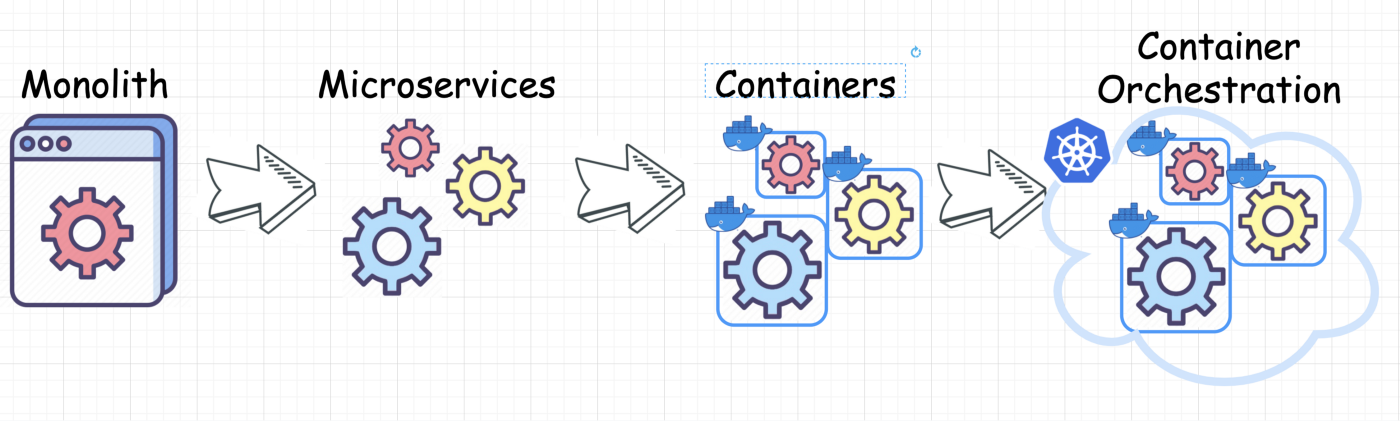
\includegraphics[width=0.8\textwidth]{resources/containerization.png}
    \caption{Architectural evolution: From monolithic applications to containerized microservices that are managed by a container orchestrator}
\end{figure}

Kubernetes operates on a cluster. A Kubernetes cluster is a set of node machines
for running containerized applications. The cluster is the heart of Kubernetes'
key advantage: the ability to schedule and run containers across a group of
machines, be they physical or virtual, on-premises or in the cloud.

\section{Kubernetes Fundamentals}


Kubernetes is an open-source orchestrator for deploying containerized
applications. It was initially developed by Google, inspired by a decade of
experience deploying scalable, reliable systems in containers via
application-oriented APIs. Since its introduction in 2014, Kubernetes has grown
to be one of the world's largest and most popular open-source projects. It has
become the standard API for building cloud-native applications in nearly every
public cloud. Kubernetes is a proven distributed system infrastructure suitable
for cloud-native developers of all scales. It provides the software necessary to
build and deploy reliable, scalable distributed systems.

\begin{figure}
	\centering
	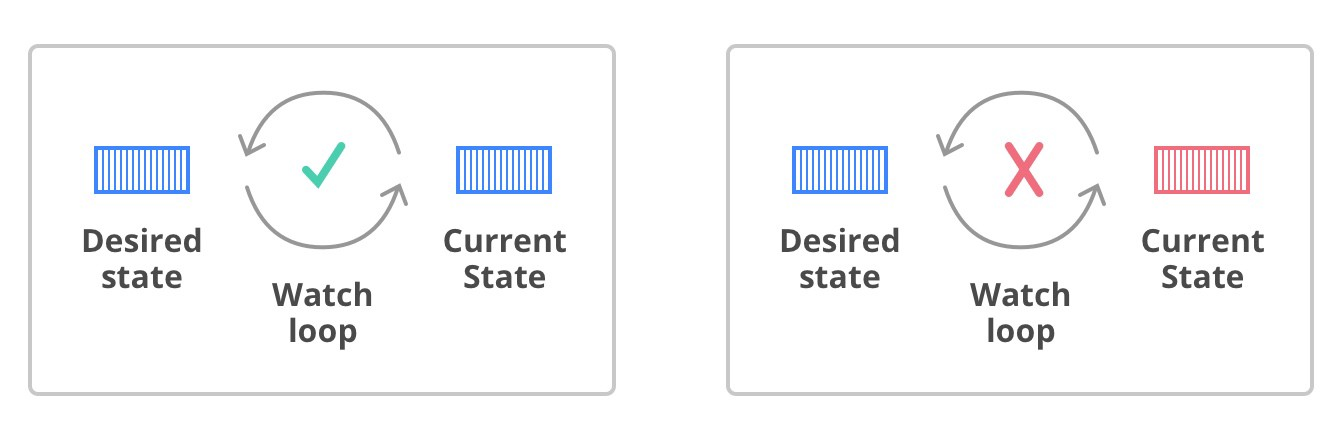
\includegraphics[width=0.8\textwidth]{resources/declarative.jpg}
	\caption{The Kubernetes reconciliation loop}
	% TODO: Replace scheme with the one from vkoukis
\end{figure}

Kubernetes makes application lifecycle management for container-based
applications much more effortless for DevOps via a declarative desired
state-based management approach. It exposes a powerful declarative API that
developers can use to describe the desired state of an application in terms of
Pods, Services, etc., and Kubernetes controllers will take immediate actions to
bring the observed state of the system to the desired state.

\subsection{Kubernetes Architecture}
A Kubernetes cluster consists of a set of worker machines, called nodes, that
run containerized applications. Every cluster has at least one worker node. The
worker nodes host the Pods, which are the components of the application
workload. The control plane manages the worker nodes and the Pods in the
cluster. In production environments, the control plane usually runs across
multiple computers, and a cluster usually runs multiple nodes, providing fault
tolerance and high availability.

\begin{figure}
	\centering
	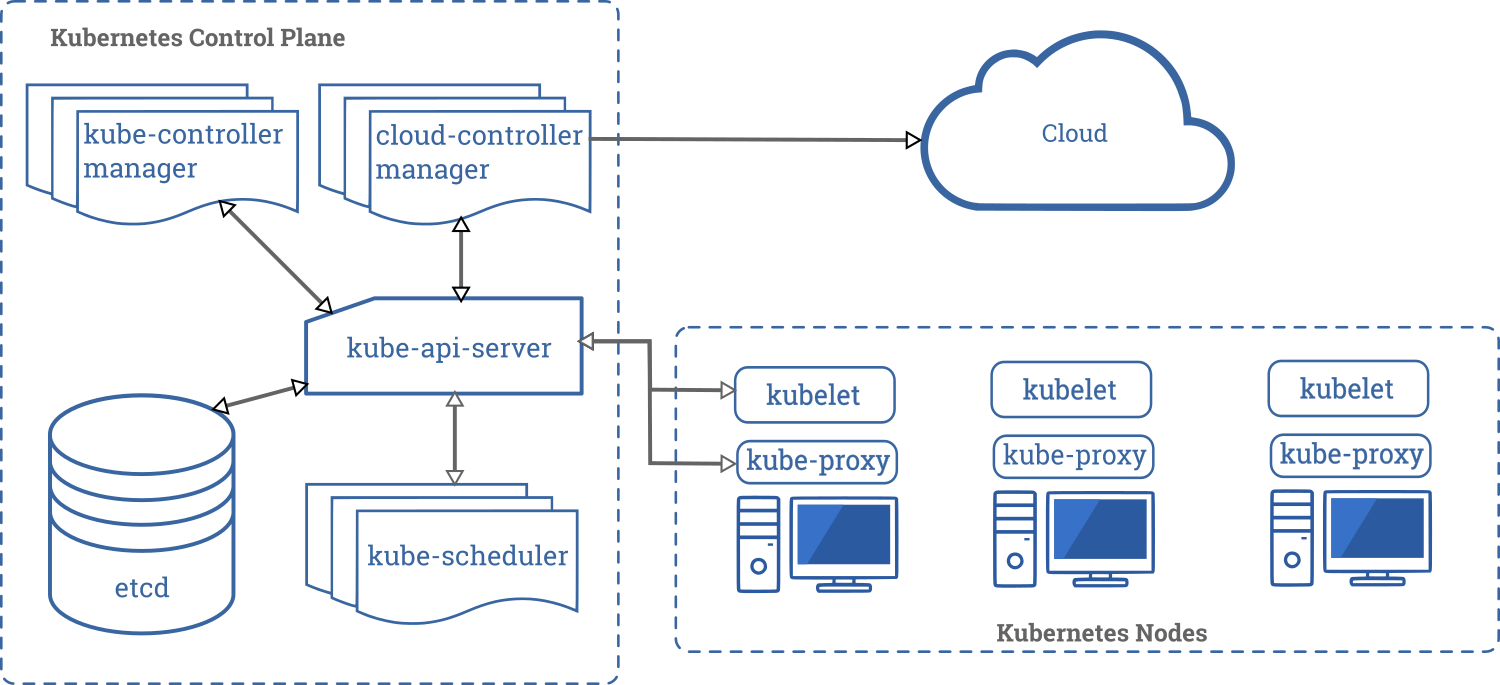
\includegraphics[width=\textwidth]{resources/components-of-kubernetes.png}
	\caption{Kubernetes Architecture}
\end{figure}


\subsection{Kubernetes Control Plane Components}
The control plane's components make global decisions about the cluster (for
example, scheduling), as well as detecting and responding to cluster events (for
example, starting up a new Pod when a deployment's replicas field is
unsatisfied).

The main control plain components are:

\begin{itemize}
	\item
	      \texttt{kube-apiserver}: The API server is a component of the
	      Kubernetes control plane that exposes the Kubernetes API. The API
	      server is the front end of the Kubernetes control plane. The primary
	      implementation of a Kubernetes API server is \co{kube-apiserver}.
	      \co{Kube-apiserver} is designed to scale horizontally, i.e., it scales
	      by deploying more instances. A cluster may run several instances of
	      \co{kube-apiserver} and balance traffic between those instances.
	\item
	      \texttt{etcd}: A consistent and highly-available key-value store that
	      is used as Kubernetes' backing store for all cluster data. Distributed
	      and fault-tolerant, etcd is an open-source, key-value store database
	      that stores configuration data and information about the state of the
	      cluster. Etcd may be configured externally, although it is often part
	      of the Kubernetes control plane.

	      Etcd stores the cluster state based on the Raft consensus algorithm.
	      This helps cope with a common problem in the context of replicated
	      state machines and involves multiple servers agreeing on values. Raft
	      defines three different roles: leader, candidate, and follower, and
	      achieves consensus by electing a leader.

	      In this way, etcd acts as the single source of truth (SSOT) for all
	      Kubernetes cluster components, responding to queries from the control
	      plane and retrieving various parameters of the state of the
	      containers, nodes, and Pods and other cluster components, in general.


	\item
	      \texttt{kube-scheduler}: Control plane component that watches for
	      newly created Pods with no assigned node and selects a node for them
	      to run on. Factors considered for scheduling decisions include
	      individual and collective resource requirements,
	      hardware/software/policy constraints, affinity, and anti-affinity
	      specifications, data locality, inter-workload interference, and
	      deadlines.
	\item
	      \texttt{kube-controller-manager}: Control plane component that runs
	      controller processes. Logically, each controller is a separate
	      process, but to reduce complexity, they are all compiled into a single
	      binary and run in a single process. Some types of these controllers
	      are:
	      \begin{itemize}
		      \tightlist
		      \item
		            \textbf{Node controller}: Responsible for noticing and
		            responding when nodes go down.
		      \item
		            \textbf{Job controller}: Watches for \co{Job} objects that
		            represent one-off tasks, then creates Pods to run those
		            tasks to completion.
		      \item
		            \textbf{Endpoints controller}: Populates the Endpoints
		            object (that is, joins Services \& Pods).
		      \item
		            \textbf{Service Account} \& \tbf{Token controllers}: Create
		            default accounts and API access tokens for new namespaces.
	      \end{itemize}
	\item
	      \texttt{cloud-controller-manager}: Kubernetes control plane component
	      that embeds cloud-specific control logic. The cloud controller manager
	      lets a user link their cluster into their cloud provider's API, and
	      separates out the components that interact with that cloud platform
	      from components that only interact with their cluster. The
	      cloud-controller-manager only runs controllers that are specific to
	      your cloud provider. If a Kubernetes cluster runs on a user's
	      premises, the cluster does not have a cloud controller manager.
\end{itemize}

\subsection{Kubernetes Node Components}

Node components run on every node, maintaining running Pods and providing the
Kubernetes runtime environment.

Every node runs the following components:

\begin{itemize}
	\item
	      \texttt{kubelet}: An agent that makes sure that containers are running
	      in a Pod.
	\item
	      \texttt{kube-proxy}: kube-proxy is a network proxy implementing part
	      of the Kubernetes Service concept. Kube-proxy maintains network rules
	      on nodes. These network rules allow network communication to the
	      user's Pods from network sessions inside or outside of their cluster.
	      Kube-proxy uses the operating system packet filtering layer if there
	      is one and it's available. Otherwise, kube-proxy forwards the traffic
	      itself.
	\item
	      \texttt{Container Runtime}: The container runtime is the software that
	      is responsible for running containers. Kubernetes supports container
	      runtimes such as containerd, CRI-O, and any other implementation of
	      the Kubernetes CRI (Container Runtime Interface).
\end{itemize}

\subsection{The Kubernetes API}

The core of Kubernetes' control plane is the API server. The API server exposes
an HTTP API that lets end-users, different cluster parts, and external
components communicate. The Kubernetes API lets the user query and manipulate
the state of API objects in Kubernetes (for example, Pods, Namespaces,
ConfigMaps, and Events). Kubernetes generally leverages common RESTful
terminology to describe the API concepts:


\begin{itemize}
	\tightlist
	\item A \textit{resource type} is the name used in the URL (Pods,
	      Namespaces, Services).
	\item All resource types have a concrete representation (their object
	      schema) which is called a \textit{kind}.
	\item A list of instances of a resource is known as a \textit{collection}.
	\item A single instance of a resource type is called a resource and usually
	      represents an object.
\end{itemize}

Almost all object resource types support the standard HTTP verbs - \texttt{GET},
\texttt{POST}, \texttt{PUT}, \texttt{PATCH}, and \texttt{DELETE}. Kubernetes
also uses its own, often written lowercase, to distinguish them from HTTP verbs.
Kubernetes uses the term ``list'' to describe returning a collection of
resources to distinguish from retrieving a single resource, usually called a
``get''. All resource types are scoped either to the cluster or to a
\textit{namespace}. A namespace-scoped resource type will be deleted when its
namespace is deleted, and access to that resource type is controlled by
authorization checks on the namespace scope.

\subsection{Kubernetes Objects}

Kubernetes \textit{objects} are persistent entities in the Kubernetes system.
Kubernetes uses these entities to represent the state of the cluster.
Specifically, they can describe:
\begin{itemize}
	\tightlist
	\item What containerized applications are running and on which nodes.
	\item The resources available to those applications.
	\item The policies around how those applications behave, such as restart
	      policies, upgrades, and fault-tolerance.
\end{itemize}

A Kubernetes object is a ``record of intent''; once a user creates the object,
the Kubernetes system will constantly work to ensure that the object exists. By
creating an object, a user is effectively telling the Kubernetes system what
they want their cluster's workload to look like.

%TODO: Add about put update delete patch
%https://kubernetes.io/docs/reference/using-api/api-concepts/

\subsubsection{The \co{Pod} Object}\label{background:Pod}

Pods  are the smallest deployable artifact in a Kubernetes cluster. A
\textit{Pod} represents a collection of application containers and volumes
running in the same execution environment. This means all of the containers in a
Pod always land on the same machine. Each container within a Pod runs in its own
cgroup, but they share several Linux namespaces. Applications running in the
same Pod share the same IP address and port space (network namespace), have the
same hostname (UTS namespace), and can communicate using native interprocess
communication channels over System V IPC or POSIX message queues (IPC
namespace). However, applications in different Pods are isolated from each
other; they have different IP addresses, different hostnames, etc. Containers in
different Pods running on the same node might also be on different servers.

\begin{figure}[ht]
	\centering
	\includegraphics[width=0.8\textwidth]{resources/Pod-lifecycle.png}
	\caption{The lifecycle of a Pod}
	% TODO: PDF
\end{figure}

\paragraph*{Phase}
The \textit{phase} of a Pod is a simple, high-level summary of where the Pod is
in its lifecycle. Each Pod follows a defined lifecycle, starting in the
\co{Pending} phase, moving through \texttt{Running} if at least one of its
primary containers starts OK, and then through either the \texttt{Succeeded} or
\texttt{Failed} phases depending on whether any container in the Pod terminated
in failure.

More specifically, the phase of a Pod can be:

\begin{itemize}
	\tightlist
	\item
	      \texttt{Pending}: the Pod has been accepted by the system, but one or
	      more of the containers has not been started. This includes time before
	      being bound to a node, as well as time spent pulling images onto the
	      host.
	\item
	      \texttt{Running}: the Pod has been bound to a node and all of the
	      containers have been started. At least one container is still running
	      or is in the process of being restarted.
	\item
	      \text	{Succeeded}: all the containers of the Pod have voluntarily
	      terminated with a container exit code of 0, and the system is not
	      going to restart any of these containers.
	\item
	      \texttt{Failed}: all the containers of the Pod have terminated, and at
	      least one container has terminated in a failure (exited with a
	      non-zero exit code or was stopped by the system).
	\item
	      \texttt{Unknown}: for some reason the state of the Pod could not be
	      obtained, typically due to an error in communicating with the host of
	      the Pod.
\end{itemize}

\paragraph*{Status}
\label{section:unschedulable-Pod}
A Pod has a \texttt{PodStatus}, which has an array of \texttt{PodConditions}
through which the Pod has or has not passed:
\begin{itemize}
	\tightlist
	\item \co{PodScheduled}: the Pod has been scheduled to a node.
	\item \co{ContainersReady}: all containers in the Pod are ready.
	\item \co{Initialized}: all init containers have completed successfully.
	\item \co{Ready}: the Pod is able to serve requests and should be added to
	      the load balancing pools of all matching Services.
\end{itemize}

\paragraph*{Unschedulable Pods}
\label{section:Pod-unschedulable}

The cluster scheduler is responsible for assigning a node for the Pod to run on.
It assigns a node by setting the \co{spec.nodeName} field of the Pod. If the
scheduler fails to find a place to run the Pod, it sets \co{PodScheduled}
\co{PodCondition} to \co{False} and reason to \co{Unschedulable}. An
unschedulable Pod will remain in \co{Pending} phase.

In the context of this thesis, we will refer to a Pod that could not be
scheduled  as ``\textit{unschedulable Pod}'' or, equivalently, ``\textit{Pending
Pod}''.
\paragraph*{Resource requests and limits}
\label{section:pod-requests}

Compute resources are measurable quantities that can be requested, allocated,
and consumed. For instance, but not limited to, CPU and memory are some types of
computing resources.

The user can specify resource requests and limits for each container of the Pod.
The scheduler uses the requests to decide which node assign to the Pod. The
kubelet uses the limits for a container and enforces them so that the running
container cannot use more of that resource than the limit a user has set. The
kubelet also reserves at least the requested amount of that system resource
specifically for that container to use. If the node where a Pod is running has
enough of that resources available, it is possible (and allowed) for a container
to use more than requested. However, a container cannot use more than the limit
of that resource.

\lstinputlisting[label={listing:pod-requests},language=yaml,caption={Requests and limits of a Pod's container}]{code/pod-requests.yaml}

\subsubsection{The \co{Node} Object}
Kubernetes runs the workload by placing Pods to run on nodes. Depending on the
cluster, a node may be a virtual or physical machine. The control plane manages
each node and contains the services necessary to run Pods. A node registered in
the Kubernetes cluster is represented using a \co{Node} object on the API
Server.

\paragraph*{Node taints}
Taints and tolerations are a mechanism that users can use to ensure that Pods
are not placed on inappropriate nodes. Taints are added to nodes, while
tolerations are defined in the Pod specification. A node can have one or many
taints associated with it. When a user taints a node, it repells all the Pods
except those that have a toleration for that taint.

% TODO: define in or define on

A taint can produce three possible effects:
\begin{itemize}
	\tightlist
	\item \co{NoSchedule}: The scheduler will only allow scheduling
	      Pods that have tolerations for the tainted nodes.
	\item \co{PreferNoSchedule}: The scheduler will try to avoid
	      scheduling Pods that don’t have tolerations for the tainted nodes.
	\item \co{NoExecute}: Kubernetes will evict the running Pods from the nodes
	      if the Pods don’t have tolerations for the tainted nodes.
\end{itemize}

\paragraph*{Node status}
\label{section:node-status}
Each \co{Node} object has a \texttt{/status} subresource that indicates the status of
the node. The status contains multiple conditions for the node and is managed by
the node controller. Some conditions that are often encountered include:

\begin{itemize}
	\tightlist
	\item \co{MemoryPressure}: If \co{True}, it indicates that the node is
	      running out of memory.
	\item \co{DiskPressure}: A \co{True} value in this field indicates that the
	      node lacks enough space.
	\item \co{PIDPressure}: If too many processes are running on the node, this
	      field will be \co{True}.
	\item \co{NetworkUnavailable}: If the network for the node is not correctly
	      configured, this will be \co{True}.
	\item \co{Ready}: If the node is healthy and ready to accept Pods, this will
	      be \co{True}. In this field, a \co{False} is equivalent to the
	      \texttt{NotReady} status in the get nodes output. It can also have the
	      Unknown value, which means the node controller has not heard from the
	      node in the last \texttt{node-monitor-grace-period}.
\end{itemize}

In the context of the Cluster Autoscaler and the Scheduler, a node will be
considered as ``\textit{Unready}''  if:
\begin{itemize}
	\tightlist
	\item It has \co{Pod.spec.unschedulable} field. This field indicates the
	      node shall not accept Pods.
	\item The \co{Node} object does not have any condition of type \co{Ready}.
	\item A condition of type \co{Ready} exists and the its status is
	      \co{False}.
	\item A condition of type \co{DiskPressure} or \co{PIDPressure} or
	      \co{NetworkUnavailable} with its corresponding status set to
	      \co{True}. exists.
\end{itemize}

The rest of the nodes shall be considered as \texttt{Ready}.

A node that cannot accept Pods will be referred to as ``\textit{unschedulable}''
node.

\paragraph*{Node allocatable}
\label{section:node-allocatable}

\textit{Allocatable} on a Kubernetes node is defined as the amount of computing
resources that are available for Pods.  The total resources (capacity) of a node
are categorized into:

\begin{itemize}
	\item \co{kube-reserved}: resource reservation for kubernetes system daemons
	      like the kubelet, container runtime, node problem detector, etc. It is
	      not meant to reserve resources for system daemons that are run as
	      Pods.
	\item \co{system-reserved}: resource reservation for OS system daemons like
	      sshd, udev, etc. system-reserved should reserve memory for the kernel
	      too since kernel memory is not accounted to Pods in Kubernetes at this
	      time.
	\item \co{eviction-threshold}: specifies limits that trigger evictions when
	      node resources drop below the reserved value.
	\item \co{allocatable}: the remaining node resources available for
	      scheduling of Pods.
\end{itemize}

\begin{figure}
	\centering
	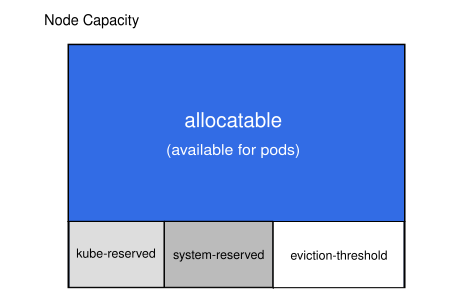
\includegraphics[width=0.7\textwidth]{resources/node-capacity.png}
	\captionof{figure}{Node resources: capacity and allocatable}
	\label{fig:test1}
\end{figure}

\subsubsection{The \co{PodDisruptionBudget} Object}
\label{section:Pod-disruption-budge}

Pods do not disappear until someone (a person or a controller) destroys them or
there is an unavoidable hardware or system software error.

The unavoidable cases are called \emph{involuntary disruptions} and include:
\begin{itemize}
	\tightlist
	\item A hardware failure of the physical machine backing the node.
	\item Cluster administrator deletes VM (instance) by mistake.
	\item Cloud provider or hypervisor failure makes VM disappear.
	\item A kernel panic.
	\item The node disappears from the cluster due to cluster network partition.
	\item Eviction of a Pod due to the node being out-of-resources.
\end{itemize}

All other cases are called \emph{voluntary disruptions}. These include both
actions initiated by the application owner and those initiated by a Cluster
Administrator. Typical voluntary disruptions include:

\begin{itemize}
	\tightlist
	\item Deleting the deployment or other controller that manages the Pod.
	\item Updating a deployment's Pod template causing a restart.
	\item Directly deleting a Pod.
	\item Draining a node for repair or upgrade.
	\item Draining a node from a cluster to scale the cluster down.
	\item Removing a Pod from a node to permit something else to fit on that
	      node.
\end{itemize}

A \texttt{PodDisruptionBudget} (PDB) limits the number of Pods of a replicated
application that are down simultaneously from voluntary disruptions. For
example, a web front end might want to ensure that the number of replicas
serving load never falls below a certain percentage of the total.

A PDB specifies the number of replicas that an application can tolerate having,
relative to how many it is intended to have. For example, a Deployment that has
a \texttt{.spec.replicas:\ 5} is supposed to have 5 Pods at any given time. If
its PDB allows for there to be 4 at a time, then the Eviction API will allow
voluntary disruption of one (but not two) Pods at a time.

Involuntary disruptions cannot be prevented by PDBs; however they do count
against the budget. Pods which are deleted or unavailable due to a rolling
upgrade to an application do count against the disruption budget.

\subsubsection{The \co{Deployment} Object}
\label{section:deployment}
A \co{Deployment} resource ensures that a specified number of Pod
\textit{replicas} are running at any time. In other words, a Deployment ensures
that a Pod or homogeneous set of Pods are always up and available. If there are
too many Pods, it will kill some. If there are too few, the Deployment will
start more.

\subsubsection{The \co{DaemonSet} Object}
\label{section:daemone-set}

A \co{DaemonSet} (DS) resource ensures that all Nodes run a copy of a Pod. As
nodes are added to the cluster, Pods are added to them. As nodes are removed
from the cluster, those Pods are garbage collected. Deleting a DaemonSet will
clean up the Pods it created.

\subsubsection{The \co{PersistentVolumeClaim} object}

A \co{PersistentVolumeClaim} (PVC, or equivalently referred to as ``claim'')) is
a request for storage by a user. Claims can request specific size and access
modes, e.g., they can be mounted \co{ReadWriteOnce}, \co{ReadOnlyMany} or
\co{ReadWriteMany}, etc.


\paragraph*{Phase}
The \textit{Phase} of a PVC can be one of the following:
\label{section:pvc-phase}
\begin{enumerate}
	\tightlist
	\item \texttt{Pending}: the PVC is not yet bound.
	\item \texttt{Bound}: the PVC is bound to a PV.
	\item \texttt{Lost}: the PVC lost its underlying PV. The claim was bound to
	      a  PV and this volume does not exist any longer and all data on it was
	      lost.
\end{enumerate}


\subsubsection{The \co{PersistentVolume} object}

A \co{PersistentVolume} (PV, or equivalently referred to as ``volume'') is a
piece of storage in the cluster that has been provisioned by an administrator or
dynamically provisioned using Storage Classes. It is a resource in the cluster.
PVs have a lifecycle independent of any individual Pod that uses the PV. This
\co{API} object captures the details of the implementation of the storage, be that
NFS, iSCSI, or a cloud-provider-specific storage system.

\begin{figure}[ht]
	\centering
	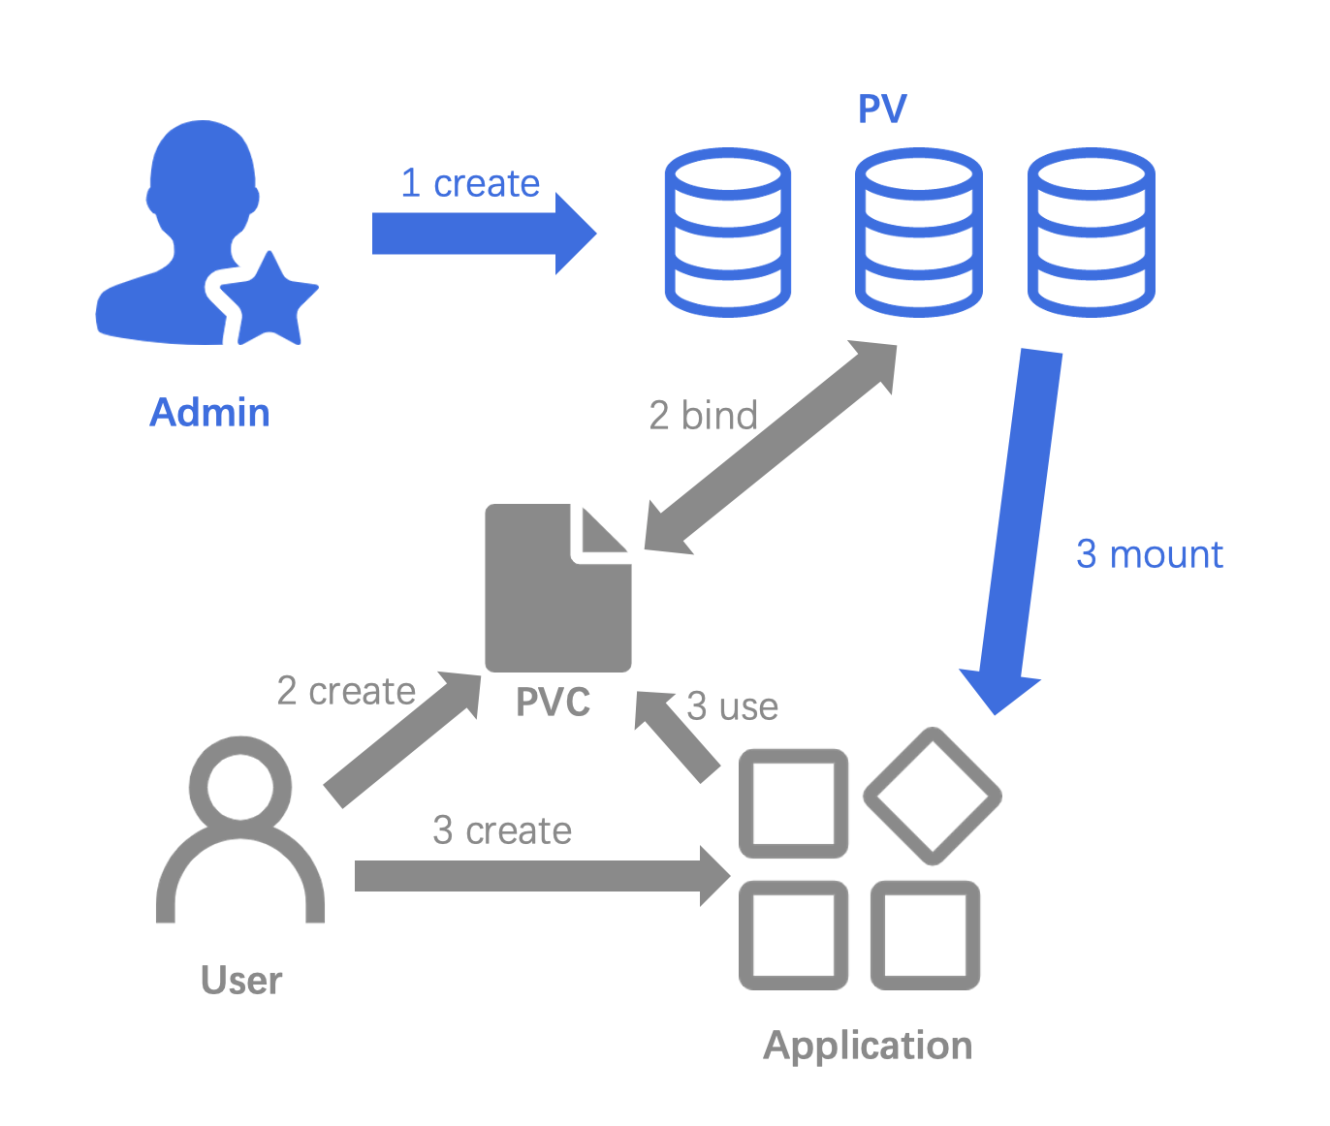
\includegraphics[width=0.6\textwidth]{resources/pvc-lifecycle.png}
	\caption{The lifecycle of a PVC and PV in the case of static provisioning}
\end{figure}

\paragraph*{Phase} A PV can be in one of the following phases:
\label{section:pv-phase}
\begin{itemize}
	\tightlist
	\item \texttt{Available}: the PV is not yet bound; it is available to be
	      matched to a PVC.
	\item \texttt{Bound}: the PV is bound to a PVC.
	\item \texttt{Released}: the PVs must be recycled before becoming available
	      again. This phase is used by the persistent volume claim binder to
	      signal to another process to reclaim the resource.
	\item \texttt{Failed}: the PV has failed to be correctly recycled or deleted
	      after being released from a claim.
\end{itemize}


\paragraph*{Binding}
PVCs are requests for storage resources; each PVC gets bound to a PV that
matches the PVC's requested storage amount and access modes. Each PV gets bound
to one PVC only, and vice versa. The binding between them is bidirectional.  A
PV will remain unbound till it is matched to a PVC. The binding is illustrated
in Figure \ref{figure:pvc-pv}.

\begin{figure}[ht]
	\centering
	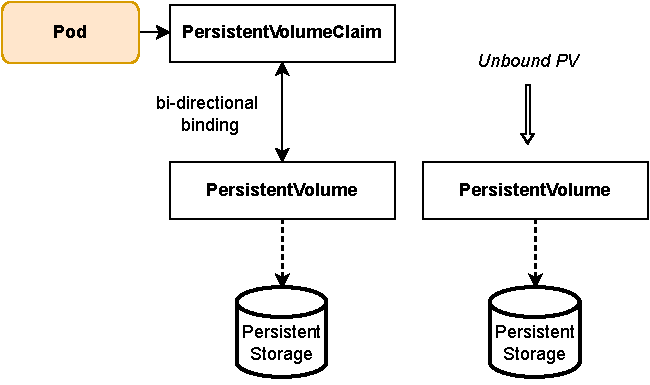
\includegraphics[width=0.8\textwidth]{resources/pvc-pv-binding.pdf}
	\caption{A Pod requests a volume using a PVC and the PVC gets bound to a PV. The PV object stores the details for the underlying persistent storage piece.}
	\label{figure:pvc-pv}
\end{figure}

The interaction between PVs and PVCs follows this lifecycle:
\begin{enumerate}
	\item \textbf{Provisioning}: There are two ways PVs may be provisioned:
	      statically or dynamically.
	      \begin{itemize}
		      \item \textbf{Statically}: A cluster administrator creates some
		            PVs. They carry the details of the actual storage, which is
		            available for use by cluster users. They exist in the
		            Kubernetes API and are available for consumption. \item
		            \textbf{Dynamically}: When none of the static PVs the
		      \item \textbf{Dynamically}: When none of the static PVs the
		            administrator created matches a user's
		            PersistentVolumeClaim, the storage system may try to
		            dynamically provision a volume for the PVC. This
		            provisioning relies on storage classes: the PVC must request
		            a storage class, and the administrator must have created and
		            configured that class for dynamic provisioning. Claims that
		            do not specify a storage class effectively disable dynamic
		            provisioning for themselves.
	      \end{itemize}
	\item \textbf{Binding}: A user creates a PersistentVolumeClaim with a
	      specific amount of storage requested and with certain access modes. A
	      control loop (the PersistentVolumeController) in the Kubernetes
	      control plane watches for new PVCs, finds a matching PV (if possible),
	      and binds them together. If a PV was dynamically provisioned for a new
	      PVC, the loop binds that PV to the PVC. Otherwise, the user will get
	      at least what they asked for, but the volume may be more than what was
	      requested. Once bound, PersistentVolumeClaim binds are exclusive,
	      regardless of how they were bound. A PVC to PV binding is a one-to-one
	      mapping, using a \co{ClaimRef} which is a bidirectional binding
	      between the PersistentVolume and the PersistentVolumeClaim. Claims
	      will remain unbound indefinitely if a matching volume does not exist.
	      Claims will be bound as matching volumes become available. For
	      example, a cluster provisioned with many 50Gi PVs would not match a
	      PVC requesting 100Gi. The PVC can be bound when a 100Gi PV is added to
	      the cluster.
	\item \textbf{Using}: Pods use claims as volumes. The cluster inspects the
	      claim to find the bound volume and mounts that volume for a Pod. For
	      volumes that support multiple access modes, the user specifies which
	      mode is desired when using their claim as a volume in a Pod. Once a
	      user has a claim and that claim is bound, the bound PV belongs to the
	      user for as long as they need it. Users access their claimed PVs by
	      including a \co{persistentVolumeClaim} section in a Pod's \co{volumes}
	      block.
\end{enumerate}

In the context of this thesis, a PVC will be also referred to as a
``\texttt{claim}''

\paragraph*{Node affinity}
\label{section:background-pv-node-affinity}

A PV can specify node affinity to define constraints that limit what nodes this
volume can be accessed from. The \co{nodeAffinity} field of the PV is a label
selector that matches nodes with the appropriate labels. Labels are key/value
pairs that are attached to objects.

The node affinity of a PV is used in the following way to indicate a volume is
local to a node:
\begin{enumerate}
	\tightlist
	\item The storage driver sets on each \texttt{Node} object a unique label.
	\item The storage driver sets the corresponding node affinity of the PV to
	      match only the unique label of the node.
\end{enumerate}

Listing ~\ref{listing:pv-affinity} presents a PV with node affinity that matches
node having the label \co{node:node-1}.

\lstinputlisting[label={listing:pv-affinity},language=yaml,caption={A PV with node affinity}]{code/node-affinity.yaml}

\subsubsection{The \co{StorageClass} Object}

A \co{StorageClass} is a Kubernetes resource that enables dynamic storage
provisioning. A StorageClass provides a way for administrators to describe the
``classes'' of storage they offer. The administrator configures the
StorageClass, which can then no longer be modified.

A storage class can specify a \co{volumeBindingMode}, which is either
\co{Immediate} or \co{WaitForFirstConsumer}:
\begin{itemize}
	\item  \co{Immediate}: Indicates that volume binding and dynamic
	      provisioning occur once the user creates the PersistentVolumeClaim.
	      For storage backends that are topology-constrained and not globally
	      accessible from all nodes in the cluster, PersistentVolumes will be
	      bound or provisioned without knowledge of the Pod's scheduling
	      requirements, possibly resulting in unschedulable Pods.
	\item \co{WaitForFirstConsumer}: The binding and provisioning of a
	      PersistentVolume will be delayed until a Pod using the
	      PersistentVolumeClaim is created. PersistentVolumes will be selected
	      or provisioned conforming to the topology that is specified by the
	      Pod's scheduling constraints.
\end{itemize}


\subsection{The Eviction API}
\label{section:background-eviction}

When deleting a resource on Kubernetes, the API server will put a
\co{deletionTimestamp} on the resource object. Unless there are any finalizers
on the object, the object will be removed from the API Server.

In the case of Pods, apart from the classic \co{DELETE} operation, Kubernetes
offers an extra API to initiate the deletion of the Pod: the \co{Eviction} API.
The main difference with the delete operation is that API-initiated evictions
respect the configured PodDisruptionBudgets and
\co{terminationGracePeriodSeconds}. So, if a user tries to \textit{evict} a Pod
and the corresponding PodDisruptionBudget does not allow the disruption of the
Pod, the Pod will not be deleted. Instead, issuing a classical \co{DELETE}
operation will remove the Pod, no matter what the PodDisruptionBudget specifies.

\subsection{The Cordon \& Drain Operations}
\label{section:cordon-drain}

The Kubernetes command-line tool, \co{kubectl}, allows a user to run commands
against Kubernetes clusters. The tool allows the complete management of the
cluster. Two essential operations used for the maintenance of the cluster are
the \textit{cordon} and the \textit{drain} operations.

\paragraph*{Cordon operation}
\textit{Cordon} is an operation offered by the \co{kubectl} CLI tool that marks
the node as \textit{unschedulable}. Marking a node as unschedulable prevents the
scheduler from placing new Pods onto that node but does not affect existing Pods
running on it. This is a preparatory step before a node reboot or other
maintenance.

The admin of the cluster can execute the cordon operation by running \co{kubectl
	cordon}. When cordoning a node, the tool adds the \textit{unschedulable
	taint} \footnote{Unschedulable taint:
	\co{node.kubernetes.io/unschedulable:NoSchedule}} on the node and also sets
	the \co{nodes.spec.unschedulable} field to \co{True}.

We will refer to the action of marking the node as unschedulable as
``\textit{cordoning the node}'' and the node as ``\textit{cordoned}''.

\paragraph*{Drain operation}

The \textit{drain} operation is used to remove workload from a node. It is run
in case the node needs maintenance, or it needs to be removed from a cluster.
The drain operation cordons the node to mark it as unschedulable, and evicts all
the Pods from the node.  Evictions allow the Pod's containers to terminate
gracefully and will respect the PodDisruptionBudgets the user has specified.

The admin of the cluster can execute the drain operation by running \co{kubectl
	drain}. If \co{kubectl drain} returns successfully, it indicates that all
	the Pods have been safely evicted (respecting the desired graceful
	termination period and the PodDisruptionBudget that is defined). It is then
	safe to bring down the node by powering down its physical machine or
	deleting its virtual machine if it runs on a cloud platform.

\section{Kubernetes Controllers}
In Kubernetes, controllers are control loops that watch the state of the
cluster, then make or request changes where needed. Each controller tries to
move the current cluster state closer to the desired state. A controller tracks
at least one Kubernetes resource type. These objects have a \co{spec} field
representing the desired state. The controllers for that resource are
responsible for making the current state come closer to that desired state.

In this section, we will describe some of the controller that play a significant
role in the storage system of Kubernetes.


\subsection{The PersistentVolume Controller}

The \co{PersistentVolumeController} is a controller that synchronizes
PersistentVolumeClaims and PersistentVolumes.  It binds PVs and PVCs and manages
their lifecycles. If the PVC references a StorageClass with static provisioning,
the control loop attempts to find a matching PV and then binds it to the PVC. In
the case of dynamic provisioning, as soon as the PV gets provisioned for the
PVC, the control loop binds them together.

\subsection{The AttachDetach Controller}

The \co{AttachDetach} controller manages volume attach and detach operations. It
looks for any Pods that get scheduled on a node and triggers the attach
operation, i.e., it creates a \co{VolumeAttachment} object to signal the
external attacher that it shall issue a \co{ControllerPublish} call to the CSI
driver. Similarly, when no Pods use a volume on a node, the controller executes
a detach operation: deletes the \co{VolumeAttachment} object to signal the external
attacher it shall issue a \co{ControllerUnpublish} request to the CSI driver.


\subsection{Kubernetes Admission Controllers}

An \textit{admission controller} is a piece of code that intercepts requests to
the Kubernetes API server prior to the persistence of the object but after the
request is authenticated and authorized. Admission controllers may be
\textit{validating}, \textit{mutating}, or both. Mutating controllers may modify
related objects to the requests they admit; validating controllers may not.

The admission control process proceeds in two phases. In the first phase, it
runs the mutating admission controllers. In the second phase, it runs the
validating admission controllers. If any controller in either phase rejects the
request, the entire request is rejected immediately and an error is returned to
the end-user.

Various admission controllers come compiled into the \co{kube-apiserver} binary,
and out of them, there are two controllers of particular interest, the
\co{MutatingAdmissionWebhook} and \co{ValidatingAdmissionWebhook}:
\begin{itemize}
      \tightlist
      \item \co{MutatingAdmissionWebhook}: This admission controller calls any
            mutating webhooks which match the request. Matching webhooks are called
            serially; each one may modify the object if desired.

      \item \co{ValidatingAdmissionWebhook}: This admission controller calls any
            validating webhooks which match the request. Matching webhooks are
            called in parallel; if any of them rejects the request, the request
            fails.
\end{itemize}

The admission controller phases are shown in Figure
~\ref{figure:admission-controller}.
\begin{figure}[ht]
      \centering
      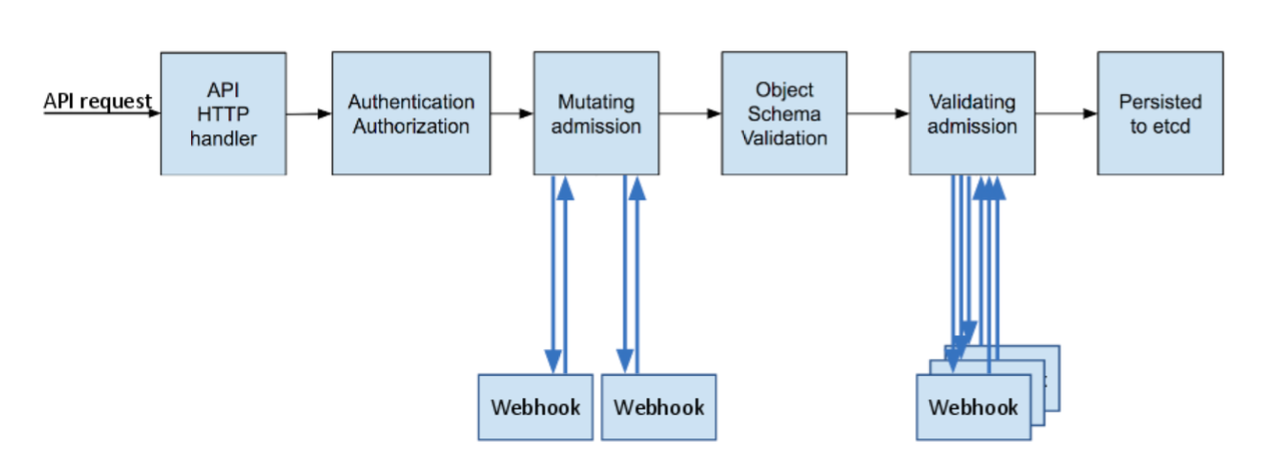
\includegraphics[width=\textwidth]{resources/admission-controller-phases.png}
      \caption{Admission controller phases}
      \label{figure:admission-controller}
\end{figure}

\section{Kubernetes Admission Webhooks}

Admission webhooks are HTTP callbacks that receive admission requests and do
something with them. Two types of admission webhooks can be defined:
\textit{validating admission} webhook and \textit{mutating admission} webhook.

Mutating admission webhooks are invoked first, and can modify objects sent to
the API server to enforce custom defaults. After all object modifications are
complete, and after the incoming object is validated by the API server,
validating admission webhooks are invoked and can reject requests to enforce
custom policies.The admin of the cluster can dynamically configure what
resources are subject to what admission webhooks via
\co{ValidatingWebhookConfiguration} or \co{MutatingWebhookConfiguration} API
objects.

\paragraph*{\co{MutatingWebhookConfiguration} Object}

Each \texttt{MutatingWebhookConfiguration} contains a list of webhooks,
specified at \co{webhooks} field. Each of the webhooks defined, may specify the
following fields:
\begin{itemize}
      \tightlist
      \item \texttt{rules}: A list of rules used to determine if a request to
            the API server should be sent to the webhook. Each rule specifies
            one or more operations, apiGroups, apiVersions, and resources, and a
            resource scope.
      \item  \texttt{failurePolicy}: Defines how unrecognized errors and timeout
            errors from the admission webhook are handled. Allowed values are
            \texttt{Ignore} or \texttt{Fail}.
      \item \texttt{namespaceSelector}:  Defines whether to run the webhook on a
            request for a namespaced resource (or a \texttt{Namespace} object) based
            on whether the namespace labels match the selector. If the object is a
            cluster scoped resource other than a Namespace, \texttt{namespaceSelector}
            has no effect.
\end{itemize}

\section{The Kubernetes Operator Pattern}
\label{section:operator-pattern}

A Kubernetes operator is a custom application-specific controller that extends
the functionality of the Kubernetes API to create, configure, and manage
instances of complex applications on behalf of a Kubernetes user. It builds upon
the fundamental Kubernetes resource and controller concepts but includes domain
or application-specific knowledge to automate the entire life cycle of the
software it manages. It uses \textit{custom resources} to manage applications
and their components. The user within a custom resource provides high-level
configuration and settings. The Kubernetes operator translates the high-level
directives into low-level actions based on best practices embedded within the
operator's logic.

A \co{CustomResourceDefinition} object (CRD) defines a custom resource and lists
out all the configurations available to users of the operator. The Kubernetes
API can handle custom resource definitions just like built-in objects, including
interaction via \co{kubectl} and inclusion in role-based access control (RBAC)
policies.

\begin{figure}[ht]
	\centering
	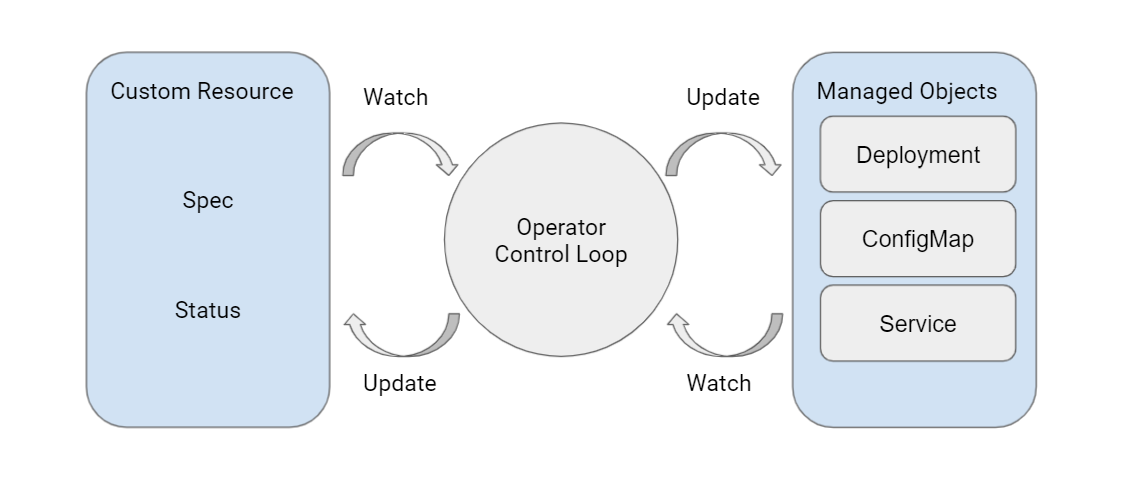
\includegraphics[width=0.8\textwidth]{resources/operator.png}
	\caption{The Kubernetes operator pattern}
\end{figure}

\section{Kubernetes Scheduler}
\RestyleAlgo{ruled}

Σε αυτήν την ενότητα, θα παρουσιάσουμε συνοπτικά τη τρέχουσα σχεδίαση του
Kubernetes Scheduler, θα επισημάνουμε τις ελλείψεις που υπάρχουν και θα
προτείνουμε βελτιώσεις που επιλύουν τους τρέχοντες περιορισμούς.

\subsection{To Πρόσθετο VolumeBinding}

Για λόγους συντομίας, στο ελληνικό τμήμα της διπλωματικής παρουσιάζουμε μόνο τη
σχεδίαση της \co{Filter} και της \co{PreBind}  φάσης του προσθέτου, καθώς
σχετίζεται άμεσα με τις προτεινόμενες επεκτάσεις. Για την αναλυτική παρουσίαση
των υπολοίπων φάσεων του προσθέτου, μπορείτε να ανατρέξετε στο αντίστοιχο
αγγλικό κεφάλαιο, στην ενότητα \ref{section:design-volume-binding}.

\subsection*{PreFilter Φάση}

\co{Filter}: αξιολογεί αν ένα Pod μπορεί να τοποθετηθεί σε έναν κόμβο, βάσει των
τόμων που ζητά, τόσο για τα δεσμευμένα όσο και για τα μη δεσμευμένα PVC:
\begin{itemize}
      \tightlist
      \item Για τα \textit{δεσμευμένα PVC}, ελέγχει ότι το PV του κάθε PVC είναι
            προσβάσιμο (βάσει τoy node affinity που φέρει) από τον εξεταζόμενο
            κόμβο.
      \item Για τα \textit{μη δεσμευμένα PVC}, προσπαθεί να βρει διαθέσιμα PVs
            που μπορούν να ικανοποιήσουν τις απαιτήσεις του PVC και που είναι
            προσβάσιμα (βάσει του node affinity τους) από τον εξεταζόμενο κόμβο.
            Τα PVCs για τα οποία δεν κατάφερε να βρει κατάλληλα PVs, θα τα
            αποκαλούμε εφεξής ``\textit{PVCs to provision}''.
      \item Για κάθε \textit{PVC to provision}, ελέγχει αν η \co{StorageClass}
            του PVC υποστηρίζει τη δυναμική παροχή και αν υπάρχει αρκετή
            χωρητικότητα αποθήκευσης προσβάσιμη από τον κόμβο. Εάν όχι, το Pod
            δεν μπορεί να ανατεθεί στον κόμβο. Αυτό είναι το βήμα όπου
            η χωρητικότητα αποθήκευσης λαμβάνεται υπόψη.

\end{itemize}

Η τρέχουσα υλοποίηση του χρονοδρομολογητή, ελέγχει αν υπάρχει αρκετή
χωρητικότητα για κάθε PVC to provision, καλώντας τη μέθοδο \co{hasEnough()} με
ένα μόνο PVC ως είσοδο. Ζητά από τον  API Server όλα τα αντικείμενα
\co{CSIStorageCapacity}. και ελέγχει αν κάποιο από αυτά ταιριάζει με το
\co{StorageClass} του PVC, είναι προσβάσιμο από τον εξεταζόμενο κόμβο και η
αναφερόμενη χωρητικότητα του αντικειμένου είναι μεγαλύτερη από τη ζητούμενη
χωρητικότητα του PVC. Εάν ένα τέτοιο CSIStorageCapacity υπάρχει, υπάρχει αρκετός
χώρος στον κόμβο για τη δυναμική παροχή τόμου για το εξεταζόμενο PVC.

Είναι σημαντικό να επισημάνουμε ότι δεν ελεγχει αν υπάρχει αποθηκευτικός χώρος
συνολικά για όλα τα PVCs, αλλά μόνο αν το κάθε PVC χωριστά χωράει σε έναν κόμβο.

\subsection*{PreBind Φάση}

Η φάση \co{PreBind} εκτελείται αφού ο χρονοδρομολογητής έχει επιλέξει έναν κόμβο
για  το Pod.

Για κάθε ένα από τα \textit{μη δεσμευμένα PVC} που το πρόσθετο βρήκε ένα
κατάλληλο PV κατά τη διάρκεια της φάσης \co{Filter}, θα ενημερώσει τον API
Server με τη δέσμευση, δηλαδή, θα ενημερώσει το αντίστοιχο PV ώστε να δείχνει
στο PVC, και στη συνέχεια, ο ελεγκτής Kubernetes PersistentVolume θα ολοκληρώσει
την αμφίδρομη δέσμευση.

Για κάθε ένα από τα \textit{PVCs to provision}, θα ενημερώσει τα αντίστοιχα PVCs
στον API Server με το  ``selected node annotation'' \footnote{Το selected node
annotation: \co{volume.kubernetes.io/selected-node}} για να σηματοδοτήσει στον
\en{external provisioner} ότι ένας τόμος για το PVC πρέπει να δημιουργηθεί δυναμικά
σε ένα τμήμα τοπολογίας που είναι προσβάσιμο από τον κόμβο που υποδεικνύει η
σημείωση. 

Στη συνέχεια, το πρόσθετο θα κάνει poll τον API Server έως ότου όλα τα PVCs
δεσμευτούν  PVs. Εάν το selected node annotation κάποιου PVC to provision
αφαιρεθεί, θα ακυρώσει την τρέχουσα προσπάθεια χρονοδρομολόγησης και θα
καλέσει τα πρόσθετα \co{Unreserve}.Η αφαίρεση του annotation είναι ένας
μηχανισμός με τον οποίο ο external provisioner ουσιαστικά ειδοποιεί τον
χρονοδρομολογητή ότι απέτυχε η παροχή του τόμου και θα πρέπει να δοκιμάσει ξανά,
ενδεχομένως σε άλλον κόμβο.


\subsection{Ελλείψεις \& Προτεινόμενες Επεκτάσεις}

Σύμφωνα με την προηγούμενη ανάλυση των αλγορίθμων, ο τρέχων σχεδιασμός του
Kubernetes Scheduler έχει τους ακόλουθους περιορισμούς:

\begin{enumerate}
      \item Η μέθοδος \texttt{Filter} του πρόσθετου VolumeBinding χρησιμοποιεί
            τα αντικείμενα \en{CSIStorageCapacity} του Kubernetes API για να
            αντλήσει πληροφορίες για τον διαθέσιμο αποθηκευτικό χώρο. Αυτό το
            αντικείμενο API έγινε beta στην έκδοση Kubernetes 1.21 και ήταν σε
            κατάσταση alpha σε προηγούμενες εκδόσεις. Οι κύριοι πάροχοι
            υπηρεσιών νέφους δεν ενεργοποιούν τα χαρακτηριστικά σε κατάσταση
            alpha στις υπηρεσίες τους. Ως αποτέλεσμα, τα CSIStorageCapacity
            αντικείμενα δεν είναι ενεργοποιημένα σε συστοιχίες που εκτελούν
            εκδόσεις προγενέστερες της 1.21 στους περισσότερους παρόχους cloud.
            Αυτό είναι ένα σημαντικό πρόβλημα, δεδομένου ότι πολλές επιχειρήσεις
            (συμπεριλαμβανομένων των πελατών μας) δεν τρέχουν τις τελευταίες
            εκδόσεις του Kubernetes για λόγους σταθερότητας. Στη δική μας
            περίπτωση, οι πελάτες μας εκτελούν συστοιχίες Kubernetes 1.19 και
            1.20 και χρειάζονταν τη δυνατότητα χρονοδρομολόγησης Pods με εξέταση
            της τοπικής αποθήκευσης.
      \item Η τρέχουσα σχεδιαστική λογική της φάσης \co{Filter} του πρόσθετου
            \co{VolumeBinding} δεν λαμβάνει υπόψη της τον αποθηκευτικό χώρο που
            απαιτείται για την παροχή πολλαπλών PVC ενός Pod. Αντ' αυτού,
            ελέγχει αν κάθε μεμονωμένο PVC μπορεί να δημιουργηθεί στον
            αποθηκευτικό χώρο που είναι προσβάσιμος από τον κόμβο, χωρίς να
            διασφαλίζει ότι υπάρχει αρκετός χώρος για όλα αυτά ταυτόχρονα. Αυτό
            είναι ένα κρίσιμο πρόβλημα: σε περίπτωση που ένα Pod αναφέρεται σε
            πολλαπλά μη δεσμευμένα PVC και δεν υπάρχει αρκετός χώρος για όλα
            αυτά, ένα από αυτά γίνει provision και η παροχή των υπολοίπων θα
            αποτύχει, τότε όλες οι μελλοντικές αποφάσεις χρονοδρομολόγησης θα
            περιορίζονται από το ήδη δημιουργημένο τόμο και το Pod θα κολλήσει.
\end{enumerate}

Δεδομένου ότι ο σχεδιασμός του upstream έρχεται με τους προαναφερθέντες
περιορισμούς, προτείνουμε να επεκτείνουμε τον Kubernetes Scheduler και να
εγκαταστήσουμε τον επεκταμένο χρονοδρομολογητή στη συστοιχία. Ο προτεινόμενος
σχεδιασμός μπορεί να χωριστεί στα ακόλουθα μέρη:

% TODO: enumerate or itemize?
\begin{enumerate}
      \tightlist
      \item Επέκταση του Rok CSI Node του οδηγού αποθήκευσης, ώστε να
            αναφέρει τη διαθέσιμη χωρητικότητα κάθε κόμβου ως annotation στο
            αντίστοιχο αντικείμενο \texttt{Node} του Kubernetes.
      \item Επέκταση του Rok CSI Controller του οδηγού αποθήκευσης
            ώστε να απαντά με κατάλληλο σφάλμα στην κλήση \co{CreateVolume} όταν
            η εναπομένουσα χωρητικότητα για την παροχή του τόμου είναι
            ανεπαρκής.
      \item Επέκταση του πρόσθετου VolumeBinding του Kubernetes Scheduler ώστε
            να ελέγχει αν πολλαπλοί τόμοι ενός Pod χωρούν σε έναν κόμβο,
            συγκρίνοντας τη συνολική τους απαίτηση σε χωρητικότητα με την
            αναφερθείσα διαθέσιμη χωρητικότητα.
      \item Εγκατάσταση του επεκταμένου χρονοδρομολογητή στη συστοιχία.
      \item Ανάπτυξη και εγκατάσταση ενός  webhook που θα μεταλλάσσει τα Pods
            ώστε να χρησιμοποιούν τον επεκταμένο χρονοδρομολογητή.
\end{enumerate}

\subsubsection{Επέκταση του Rok CSI Node}

Δεδομένου ότι τα αντικείμενα \co{CSIStorageCapacity} δεν μπορούν να γίνουν
back-port σε προηγούμενες εκδόσεις του Kubernetes και, επίσης, η προσθήκη ενός
παρόμοιου Custom Resource θα απαιτούσε αρκετή προσπάθεια άνευ αιτίας,
αποφασίζουμε να αναφέρουμε τη χωρητικότητα κάθε κόμβου ως annotation στο
αντίστοιχο αντικείμενο Node. Το annotation, το οποίο αποκαλούμε ``annotation
χωρητικότητας'' θα είναι της μορφής
\co{rok.arrikto.com/capacity:<free-storage-bytes>}.

Το πρόσθετο Rok CSI Node του οδηγού αποθήκευσης που εκτελείται σε κάθε κόμβο της
συστοιχίας υπολογίζει περιοδικά τον διαθέσιμο αποθηκευτικό χώρο και ενημερώνει
το annotation χωρητικότητας. Δίνει εντολές στο Logical Volume Manager (LVM) του
κόμβου για να μάθει τον ελεύθερο χώρο του Rok Volume Group και ενημερώνει το
αντίστοιχο \co{Node} αντικείμενο με την τιμή της διαθέσιμης χωρητικότητας.

\subsubsection{Επέκταση του Rok CSI Controler}

Επεκτείνουμε το πρόσθετο Rok CSI Controller του οδηγού αποθήκευσης ώστε να
επιστρέφει το status  code \co{GRPCResourceExhausted} ως απάντηση στην κλήση
\co{CreateVolume} του external provisioner όταν η παροχή ενός τόμου αποτυγχάνει
λόγω ανεπαρκούς χωρητικότητας αποθήκευσης.

\subsubsection{Επέκταση του VolumeBinding Plugin}
\label{section:gr-volume-plugin-extensions}

Προτείνουμε την επέκταση της \co{Filter} μεθόδου του πρόσθετου
\co{VolumeBidning} ως εξής:
\begin{enumerate}
      \tightlist
      \item Κατά τον έλεγχο των PVCs του Pod που χρειάζονται να δημιουργηθούν
            δυναμικά (provision) (μέθοδος \co{checkVolumeProvisions()}), να
            επιλέγει όλα τα Rok PVCs
            \footnote{PVCs provisioned by the \co{rok.arrikto.com}
                  provisioner.} (εφεξής αναφέρονται ως ``\\textit{Rok claims to
                  provision}'') και να ελέγχει αν υπάρχει αρκετή χωρητικότητα
                  για το συνολικό αποθηκευτικό χώρο που ζητούν.
      \item Να ελέγχει αν υπάρχει αρκετή χωρητικότητα για τα Rok claims to
            provision ως εξής:
            \begin{enumerate}
                  \tightlist
                  \item Να υπολογίζει τη συνολική χωρητικότητα που ζητείται
                        αθροίζοντας τα αιτήματά τους.
                  \item Να ελέγχει  αν ο εξεταζόμενος κόμβος διαθέτει annotation
                        χωρητικότητας του Rok \footnote{Το annotation
                        χωρητικότητας του Rok:
                        \texttt{rok.arrikto.com/capacity}} .
                  \item Αν to annotation \textit{δεν υπάρχει}, ή αν υπάρχει αλλά
                        δεν είναι έγκυρος ακέραιος αριθμός, τα Rok claims to
                        provision δεν μπορούν να δημιουργηθούν στον κόμβο. Η
                        απουσία της σημείωσης υποδεικνύει ότι το πρόγραμμα
                        οδήγησης Rok CSI δεν εκτελείται στον κόμβο.
                  \item Εάν υπάρχει το annotation χωρητικότητας, να ελέγχει αν η
                        αναφερόμενη διαθέσιμη χωρητικότητα είναι μεγαλύτερη ή
                        ίση με τη συνολική χωρητικότητα που ζητούν τα Rok claims
                        to provision. Εάν δεν ισχύει η συνθήκη, δεν υπάρχει
                        αρκετή χωρητικότητα, και τα Rok claims to provision δεν
                        μπορούν να δημιουργηθούν στον κόμβο,  οπότε και το Pod
                        δεν μπορεί να προγραμματιστεί στον κόμβο.
            \end{enumerate}
      \item Διατηρούμε της συμβατότητα προς τα πίσω με τη μη τροποποίηση του
            χειρισμού των  PVCs που δεν ζητούν αποθηκευτικό χώρο από την κλάση
            αποθήκευσης Rok. Ο σχεδιασμός μας, διαχωρίζει τα PVCs σε τοπικά Rok
            PVCs και μη Rok PVCs, και επεκτείνει μονάχα τον τρόπο χειρισμού
            μονάχα για τα Rok PVCs. Τα PVC που παρέχονται από άλλους παρόχους
            αποθήκευσης δεν θα επηρεαστούν από τις αλλαγές μας.
\end{enumerate}

% transl: επιπεδο ελέγχου


\subsubsection{Εγκατάσταση του Rok Scheduler}

Ο \co{kube-cheduler} εκτελείται από προεπιλογή σε κάθε πάροχο νέφους ως μέρος
του επιπέδου ελέγχου του Kubernetes και είναι ο προεπιλεγμένος χρονοδρομολογητής
που χρησιμοποιείται για τη χρονοδρομολόγηση των Pods. Οι πάροχοι νέφους
αποκρύπτουν το επίπεδο ελέγχου από τον τελικό χρήστη των υπηρεσιών τους, οπότε
δεν υπάρχει δυνατότητα αντικατάστασης και παραμετροποίησης του εκτελούμενου
χρονοδρομολογητή.

Ως συνέπεια αυτού του περιορισμού, εγκαθιστούμε στη συστοιχία --παράλληλα με τον
προεπιλεγμένο χρονοδρομολογητή--  τον δικό μας χρονοδρομολογητή, που εκτελεί το
επεκταμένο  VolumeBinding πρόσθετο.  Εφεξής θα αναφερόμαστε στον δικό μας
επεκταμένο χρονοδρομολογητή ως ``\textit{Rok Scheduler}''.

\subsubsection{Εγκατάσταση του Rok Scheduler Webhook}

Δεδομένου ότι εγκαθιστούμε τον Rok Scheduler χωρίς να αντικαταστήσουμε το
προεπιλεγμένο Kubernetes Scheduler της συστοιχίας, κάθε Pod πρέπει να καθορίζει
ποιος scheduler θα το χρονοδρομολογήσει ορίζοντας το πεδίο
\co{spec.schedulerName}. Εάν το πεδίο δεν έχει οριστεί, ο προεπιλεγμένος
χρονοδρομολογητής χρησιμοποιείται.

Σίγουρα δεν θέλουμε κάθε χρήστης να ορίζει χειροκίνητα το όνομα του scheduler
στο το Pod - αυτό θα επέτρεπε στους χρήστες να παρακάμψουν την πολιτική
χρονοδρομολόγησης που έχουμε ορίσει, είναι επιρρεπές σε σφάλματα και είναι μια
κουραστική διαδικασία. Χρειαζόμαστε έναν αυτόματο τρόπο για να το πετύχουμε
αυτό. Η λύση για την αυτοματοποίηση της εργασίας, είναι ένα mutating webhook.

Εγκαθιστούμε ένα μεταλλασσόμενο webhook στη συστοιχία, το οποίο στο εξής θα
αναφέρεται ως ``\textit{Rok Scheduler webhook}'', το οποίο δέχεται τα πρόσφατα
δημιουργηθέντα Pods σε συγκεκριμένα namespaces της συστοιχίας και τα
μεταλλάσσει προσθέτοντας το όνομα του Rok Scheduler στο πεδίο
\co{spec.schedulerName}.
\section{Kubernetes Cluster Autoscaler}
\label{section:autoscaler}
\RestyleAlgo{ruled0}

In this section, we are going to expose the design of the Cluster Autoscaler
(Autoscaler), describe its main principles of operation, identify its
limitations and propose extensions that will enable its seamless operation with
local persistent volumes.


\subsection{Fundamental terms}

Before we describe the algorithms of operations of the Autoscaler, it is
essential to understand some fundamental structures and terminology it uses.

\subsubsection{The Node Group Abstraction}

The Autoscaler uses the abstraction of a ``\textit{node group}''. A node group
is not an actual Kubernetes resource but rather an abstraction for a group of
nodes within a cluster. The Autoscaler expects that nodes found within a single
node group have the same resources (CPU, memory, storage) and share several
common properties such as labels and taints. However, they can still
differentiate in some details, e.g., they may consist of more than one
availability zone.

Each node group has the following important properties:
\begin{itemize}
      \tightlist
      \item \co{minSize}:minimum size of the node group.
      \item  \co{maxSize}: maximum size of the node group.
      \item  \co{targetSize}: the target size of the node group.
\end{itemize}

% TODO: Diagram TODO: PVC PV term TODO: All figures dots or not

\subsubsection{The \texttt{CloudProvider} Interface}

The Autoscaler operates with various cloud providers, e.g., GCE, AWS. To achieve
this, it specifies two important interfaces that each cloud provider that aims
to integrate its services with the Autoscaler must implement:
\begin{itemize}
      \tightlist
      \item The \co{CloudProvider} interface:  it contains configuration info
            and functions for interacting with the cloud provider.
      \item The \co{NodeGroup} interface: it contains configuration info and
            functions to control a node group.
\end{itemize}

The \co{NodeGroup} interface builds upon the node group abstraction. Each cloud
provider may choose its interpretation of what is a node group on its service,
as long as it conforms with the abstraction's definition.

For example, in the case of AWS EKS, the implementation of the \co{NodeGroup}
interface maps each node group to an AWS Auto Scaling Group (ASG). An Auto
Scaling group contains a collection of Amazon EC2 instances that are treated as
a logical grouping for automatic scaling and management purposes. An EC2
instance is a virtual server in Amazon Web Services terminology. A cluster
administrator configures the Auto Scaling groups of the EKS cluster and sets
their \co{minSize}, \co{maxSize} accordingly. The Autoscaler interacts with the
AWS cloud provider through the \co{CloudProvider} interface, which (the
CloudProvider interface) lists the configured Auto Scaling groups and maps each
of them to a node group. Only the \co{CloudProvider} interface knows about ASGs;
the rest components of the Autoscaler are unaware of the underlying
implementation and only see node groups.


\subsubsection{The \texttt{ClusterSnapshot} Interface}

The Autoscaler runs simulations on the cluster to make decisions. It takes a
snapshot of the current cluster, adds or removes nodes in the snapshot, and
simulates the scheduling decisions on the modified snapshot. A cluster snapshot
contains a fixed view of the cluster's nodes and the Pods that run on each node.
The \co{ClusterSnapshot} interface describes methods for taking a snapshot of
the cluster nodes and their Pods.

Note that the cluster's PVCs and PVs are not contained in the snapshot. Instead,
they are fetched from the API Server by the VolumeBinding plugin when the
\co{PredicateChecker} checks if a Pod can be placed on a node. We will explain
more about this later on.

\subsubsection{The \texttt{PredicateChecker} interface}

The Autoscaler defines the \co{PredicateChecker} interface, which offers methods
to check whether all required predicates pass for a given Pod and node.

A Predicate is equivalent to a \co{Filter} plugin (see section
\ref{section:background_scheduling_framework}) and it is used to filter out
nodes that can not run a Pod.

These are the methods of the interface:
\begin{itemize}
      \tightlist
      \item \co{CheckPredicates()}: checks if the given Pod can be placed on the
            given node.
      \item \co{FitsAnyNode()}: checks if the given Pod can be placed on any of
            the given nodes.
      \item \co{FitsAnyNodeMatching()}: checks if the given Pod can be placed on
            any of the given nodes matching the provided function.
\end{itemize}


The Autoscaler implements this interface. The implementation is called
\co{SchedulerBasedPredicateChecker} and leverages the Kubernetes Scheduler code.
In particular, the Autoscaler imports the code of the Kubernetes Scheduler and
constructs a list of predicates from the \co{Filter} plugins of the Scheduler.
The Autoscaler uses the \co{SchedulerBasedPredicateChecker} in its simulations
to determine whether a Pod can be placed on a node or not. The methods of the
interface it implements follow this basic flow:
\begin{enumerate}
      \tightlist
      \item Create a new scheduler \co{CycleState}.
      \item Run the \co{preFilter} method of all the plugins. Note that in the
            case of the VolumeBinding plugin, this step fetches the PVCs and PVs
            of the Pod from the API Server and stores them in the
            \co{CycleState}.
      \item Runs all the \co{Filter} plugins to determine if the Pod can be
            placed on the node.
\end{enumerate}

At this point, we shall highlight the fact that the Autoscaler imports the code
of the Kubernetes Scheduler and uses the \co{Filter} plugins it provides in the
\co{SchedulerBasedPredicateChecker} to run a simulation. However, it
\textbf{never} interacts with the live instance of the Kubernetes Scheduler that
runs on the cluster.

\subsubsection{The \texttt{Estimator} \& \texttt{Strategy} Interfaces}

The Autoscaler specifies two interfaces that are used in the scale-up procedure:
\begin{itemize}
      \tightlist
      \item \co{Estimator}: interface for calculating the number of nodes of a
            given type needed to schedule Pods.
      \item \co{Strategy}: interface for selecting the best option to scale up.
\end{itemize}


The estimator currently used by the Autoscaler is \co{BinPackingNodeEstimator}.
This estimator implements the First Fit Decreasing bin packing approximation
algorithm.

%TODO: Bin packing

\subsubsection{Template Nodes}
\label{section:design-template}

As we have explained, the Autoscaler assumes that every node in a node group
will have the same resources (CPU, memory, storage) and labels. It constructs a
template node for each node group to add it to the cluster snapshot and run its
simulations. As the name suggests, a template node represents the details of a
new node of the given node group. A template node is a \co{NodeInfo} struct and
contains the details of a real \co{Node} object and information about the DaemonSet
Pods that would run on the node if it was an actual node in the cluster. The
Autoscaler tries to build a template node of a node group as follows:

\begin{enumerate}
      \tightlist
      \item First, look for a ready and schedulable node of the node group in
            the cluster and use it to generate the template.
      \item If the previous step failed, look for a template in the Cluster
            Autoscaler's cache.
      \item If the previous step failed, call the cloud provider's compiled
            plugin to generate a template for the given node group.
      \item If the previous step failed, look for any unready or unschedulable
            node of the given node group in the cluster and use it to generate
            the template.
\end{enumerate}


The constructed template nodes are \textit{sanitized}: the sanitization is a
mechanism that removes irrelevant or undesired details from the constructed node
template, such as the name of the node, specific labels, etc.

The complete algorithm for template node creation is shown in
Algorithm~\ref{alg:template} and the algorithm for the node template
sanitization in Algorithm~\ref{alg:sanitize-template}.


\begin{algorithm}[H]
    \caption{Cluster Autoscaler: GetNodeInfoForGroup() method}\label{alg:template}
    \KwIn{node group: A NodeGroup struct.}
    \KwOut{A template node for the Node Group (NodeInfo struct).}
    \begin{enumerate}[leftmargin=0.5cm]
        \tightlist
        \item \If{a ready and schedulable node of the node group exists
                  in the cluster}{
                  \begin{enumerate}
                      \tightlist
                      \item Build the template from that node.
                      \item Store the template in the template's cache.
                      \item Return the template.
                  \end{enumerate}
              }
        \item \If{a template node for the node group exists in the Autoscaler's cache}{
                  \begin{enumerate}
                      \tightlist
                      \item Return the cached template node.
                  \end{enumerate}
              }
        \item Call \co{TemplateNodeInfo()} of the \co{NodeGroup} interface to
              get the cloud provider defined template for the node group.
        \item \If{the \co{TemplateNodeInfo()} generated the template successfully}{
                  \begin{enumerate}
                      \tightlist
                      \item Return the template.
                  \end{enumerate}
              }
        \item \If{an unready or unschedulable node of the node group exists
                  in the cluster}{
                  \begin{enumerate}
                      \tightlist
                      \item Build the template from that node.
                      \item Return the template.
                  \end{enumerate}
              }
        \item
              Return error, the template node could not be constructed.
    \end{enumerate}
\end{algorithm}
\clearpage
\begin{algorithm}[H]
\caption{Cluster Autoscaler: sanitizeNodeInfo() method}\label{alg:sanitize-template}
\KwIn{\co{node}: A template node (\co{NodeInfo} struct)}
\KwOut{A sanitized template node (\co{NodeInfo} struct).}
\begin{enumerate}
    \tightlist
    \item \co{nodeName} \lar \co{``template-node-for-<nodegroup-name>-<random-suf>''}.
    \item Set the \co{kubernetes.io/hostname} label of the node to \co{nodeName}
    \item Remove the following taints of the node:
      \begin{itemize}
        \tightlist
        \item \co{ToBeDeletedByClusterAutoscaler}
        \item \co{DeletionCandidateOfClusterAutoscaler}
        \item any taints that indicate the node's condition, e.g,
          \co{node.kubernetes.io/not-ready}
      \item taints starting with the \co{ignore-taint.cluster-autoscaler.kubernetes.io/} prefix.
      \end{itemize}
    \item Remove any taints of the node, as specified by the \co{--ignore-taints} flag of the Cluster Autoscaler.
    \item Return the sanitized node.
\end{enumerate}
\end{algorithm}

\subsubsection{Node Utilization}

As for scale-down, the Autoscaler acts based on a metric called the utilization
of a node; it calculates this metric using the \emph{resource requests} of the
Pods that run on the node instead of any actual (live) resource metrics.

Each Kubernetes node may have multiple resources, such as CPU, memory, etc. The
cluster Autoscaler computes the utilization of every node in the cluster. For a
given resource and node, the utilization is the ratio of the total resource
requests from the Pods running on the node over the resource allocatable of the
node. The utilization is a float number ranging from 0 to 1, where 1 indicates
full utilization and 0 no utilization.

For example, the CPU utilization is defined as:
\[ node\_cpu\_utilization  =  \frac{total\ CPU\ requests\ of\ Pods\ running\ on\
            the\ node }{ allocatable\ cpu\ of\ the\ node} \]

The steps for calculating the utilization of a node are shown in
Algorithm~\ref{alg:utilization}.

\begin{algorithm}[H]
\SetEndCharOfAlgoLine{.}
\caption{Cluster Autoscaler: CalculateUtilization() method}\label{alg:utilization}
    \KwIn{\co{node}: A Node API object
    \\ \co{pods}: the Pods running on the node
    \\ \co{resource}: a specific resource type, e.g, cpu, memory, etc
    }
    \KwOut{The utilization of node for a given resource}
    \begin{enumerate}[leftmargin=0.5cm]
        \tightlist
        \item  Get the node allocatable resource from the \co{Node} object:\\ \texttt{nodeAllocatable} \(\leftarrow\) \texttt{node.Status.Allocatable[resource]}.
        \item \lIf{nodeAllocatable == 0}{\Return 0}
        \item Initialize: \texttt{daemonSetRequests} \lar 0, \texttt{podRequest \lar 0}.
        \item Calculate the Pods' total resource requests. For each \co{pod} in \co{pods}: 
            \begin{enumerate}
            \tightlist
            \item \texttt{request} \lar  Calculate the resource request of the Pod by summing the
                \texttt{container.Resources.Requests{[}resourceName{]}} of each container of the
                \co{pod}.
            \item \lIf{Autoscaler is configured to ignore DaemonSet
                Pods in node utilization AND the Pod is a
                DaemonSet Pod}{
                \texttt{daemonSetRequests+= request}}
            \item \lIf {the Pod is long terminating}{continue to next Pod}
            \item \texttt{podRequest += request}.
            \end{enumerate}
    \item Calculate the utilization: \[ utilization =  \frac{podRequest - daemonSetRequests}{ nodeAllocatable - daemonSetRequests} \]
    \item \Return{utilization} 

    \end{enumerate}
\end{algorithm}
% TODO: Mirror long terminating 



\subsection{The Main Loop}
The Autoscaler runs continuously a loop, called the \textit{main loop}, which
executes two basic operations on the cluster:

\begin{itemize}
      \tightlist
      \item \textit{Scale-up}: adding new nodes to cluster to help unschedulable
            Pods.
      \item \textit{Scale-down}: removing unneeded nodes from a cluster.
\end{itemize}

The steps of the Autoscaler's main loop are shown in
Algorithm~\ref{alg:template}.

\clearpage
\begin{algorithm}[H]
  \caption{Cluster Autoscaler: The main loop - RunOnce() method}\label{alg:autoscaler-main-loop}
  \begin{enumerate}[leftmargin=0cm]
    \tightlist
    \item
          \texttt{unschedulablePods} \lar Select Pods that do not have \texttt{spec.nodeName} set.
    \item
          \texttt{scheduledPods} \lar Select Pods that have \co{spec.nodeName} set.
    \item
          \texttt{allNodes} \lar List all the nodes of the cluster, by calling \co{ObtainNodesList()}.
    \item
          \texttt{readyNodes} \lar List the Ready nodes of the cluster, by calling \co{ObtainNodesList()}.

    \item
          \co{nodeGroups} \lar List the registered node groups of the cluster from the cloud provider.
    \item
          Take a snapshot of the cluster.
    \item
          For every node group in \co{nodeGroups}, generate its template node.
    \item For each node group in \co{nodeGroups} calculate the number of
          upcoming nodes (nodes that the Autoscaler has asked to be added but
          are not yet in the cluster) and add the same number of the node
          group's template nodes in the cluster snapshot.
    \item
          Run a scheduling simulation with the current cluster snapshot to determine if any of the \texttt{unschedulablePods} can be scheduled on the upcoming nodes.
    \item \lIf{any Pod in \co{unschedulablePods} is considered as schedulable in
            the simulation}{disable the scale-down for the current loop}
    \item \co{unschedulablePodsToHelp} \lar Pods from \co{unschedulablePods} that remained unschedulable in the simulation.
    \item \lIf{\co{unschedulablePodsToHelp} is empty}{do not scale-up}
    \item
          Else, try to scale-up, by calling \co{ScaleUp()}.
    \item
          \lIf{no scale-up was attempted}{proceed with the scale-down evaluation}
  \end{enumerate}
\end{algorithm}

\clearpage
\begin{figure}[H]
      \centering
      \makebox[\textwidth][c]{
            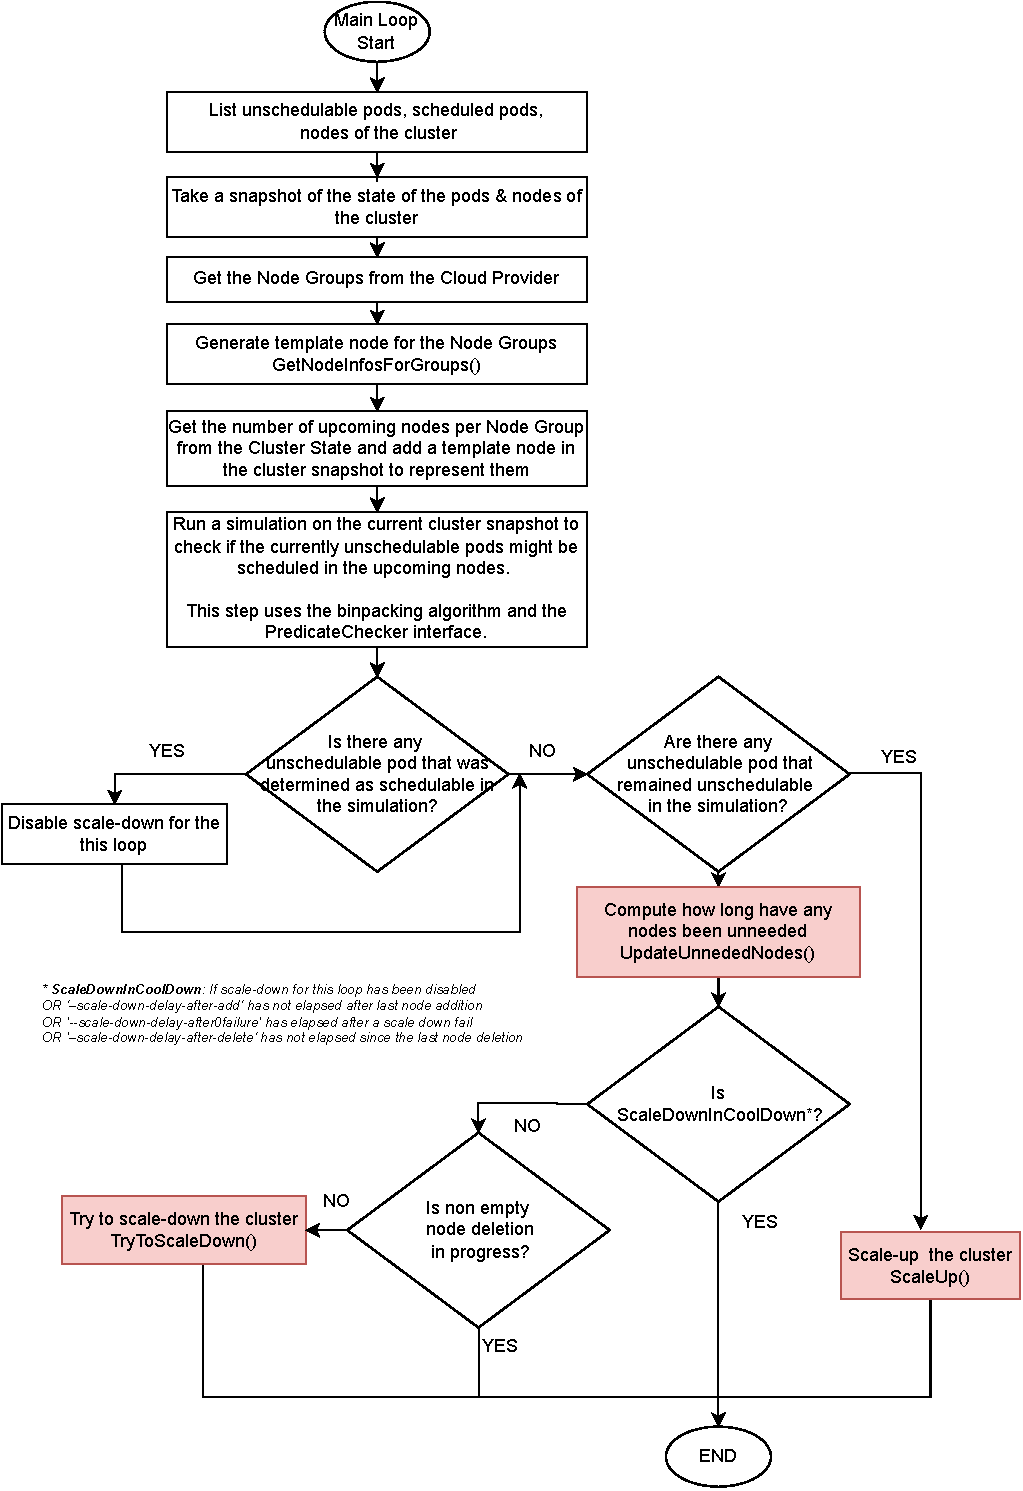
\includegraphics[width=\textwidth]{resources/autoscaler-main-loop.pdf}
      }
      \caption{Cluster Autoscaler:The main loop}
      \label{figure:autoscaler-main-loop}
\end{figure}


\subsection{Scale-Down}
\label{section:design-scale-down}
The Autoscaler tries to scale down the cluster if it did not attempt any
scale-up in the current run of the main loop. The scale-down procedure consists
of two distinct procedures:
\begin{enumerate}
      \tightlist
      \item \textit{Update unneeded nodes}: calculates which nodes have been
            unneeded and for how long.
      \item \textit{Try to scale down}: attempts to scale down the cluster by
            removing unneeded nodes.
\end{enumerate}

\begin{figure}[H]
      \centering
      \makebox[\textwidth][c]{
            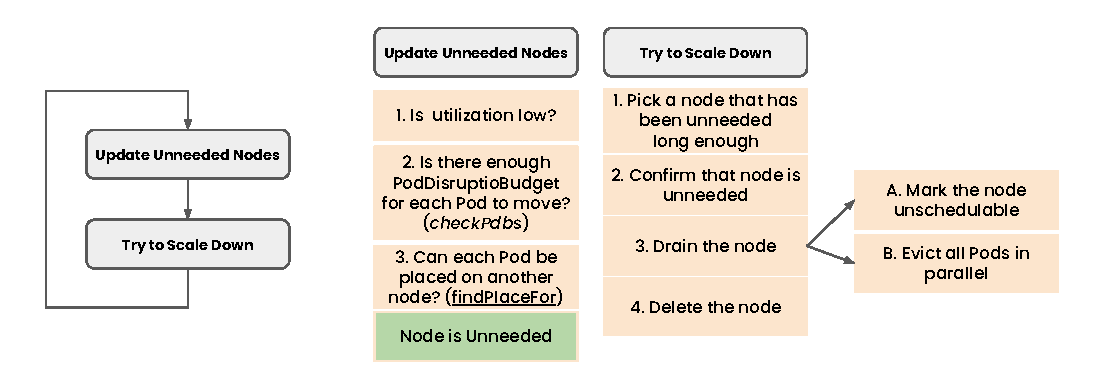
\includegraphics[width=1.1\textwidth]{resources/autoscaler-scale-down-process.pdf}
      }
      \caption{Cluster Autoscaler: Scale-down procedure}
      \label{figure:autoscaler-scale-down}
\end{figure}

We will use symbolic names to refer to various parameters of the Autoscaler in
our analysis, presented in Table \ref{table:symbolic-names-autoscaler}.
\begin{table}
      \begin{tabularx}{\linewidth}{|L|L|}
            \hline
            \textbf{Symbolic Name}        & \textbf{Description}                 \\ \hline
            scanInterval                  & How often cluster is reevaluated for
            scale up or down.
            \\
            \hline
            scaleDownDelayAfterAdd        & How long after scale up that scale
            down evaluation resumes. Defaults to 10 minutes. Configurable via
            the \co{--scale-down-delay-after-add} flag.                          \\
            \hline

            scaleDownDelayAfterDelete     & How long after node deletion that
            scale down evaluation resumes. Defaults to scanInterval.
            Configureable via the \co{--scale-down-delay-after-delete} flag.      \\
            \hline

            scaleDownDelayAfterFailure    & How long after scale down failure
            that scale down evaluation resumes. Defaults to 10 minutes.
            Configurable via the \co{--scale-down-delay-after-failure} flag.     \\
            \hline

            scaleDownUtilizationThreshold & Utilization threshold below which a
            node can be considered for scale down. Defaults to 0.5. Configurable
            via the \co{--scale-down-utilization-threshold} flag.                \\
            \hline

            scaleDownUnneededTime         & How long a ready node should be
            unneeded before it is eligible for scale down.  Defaults to 10
            minutes. Configurable via the \co{--scale-down-unneeded-time} flag.
            \\
            \hline

            scaleDownUnreadyTime          & How long an unready node should be
            unneeded before it is eligible for scale down.  Defaults to 20
            minutes. Configurable via the \co{--scale-down-unready-time} flag.
            \\
            \hline
      \end{tabularx}
      \caption{Symbolic names for various parameters of the Autoscaler used in our analysis}
      \label{table:symbolic-names-autoscaler}
\end{table}


\subsubsection{Update Unneeded Nodes Procedure}
The \textit{update unneeded nodes} procedure calculates which nodes of the
cluster have been unneeded and updates the Autoscaler's internal state with the
duration they have been unneeded. The Autoscaler considers a node
\textit{unneeded} if it meets all the following criteria:
\begin{itemize}
      \tightlist
      \item It is \textit{underutilized}, i.e., it has resource utilization
            below a specific threshold.
      \item The Pods that run on the node can be evicted (see section
            \ref{section:background-eviction}), i.e., their eviction is not
            blocked by any PodDisruptionBudgets.
      \item The Pods that run on the node can be moved to a different cluster
            node.
\end{itemize}
If a node does not meet the criteria, it is considered \textit{unremovable}.

To determine if an underutilized node is unneeded, the Autoscaler runs these
steps:
\begin{enumerate}
      \tightlist
      \item Calculate the Pods that must be moved if it removes the node.
      \item Check if any PodDisruptionBudgets block the eviction of any Pod. If
            so, the node is unremovable.
      \item Call \co{FindPlaceFor()} to find place for the Pods on a different
            node. \co{FindPlaceFor()} uses the
            \co{SchedulerBasedPredicateChecker} interface to determine if the
            Pod can be placed on any other node. It checks if the Pod can fit a
            node due to other scheduling constraints (CPU, memory), as well as
            if the Pod's volumes can be accessed from the node.
\end{enumerate}


The steps for  calculating the unneeded nodes are shown in
Algorithm~\ref{algo:update-unneeded}.

\subsubsection{Try to Scale Sown Procedure}

If a \textit{Ready} node remains unneeded for longer than
\co{scaleDownUnneededTime}, or an \textit{Unready} node remains unneeded for
longer than \co{scaleDownUnreadyTime} (see Table
\ref{table:symbolic-names-autoscaler} for the symbolic names) the Autoscaler
will consider the node as a candidate for deletion.

The Autoscaler makes a distinction between non-empty and empty nodes:
\begin{itemize}
      \tightlist
      \item \textit{Empty nodes}: nodes that run \textit{only} DaemonSet Pods.
            The Autoscaler removes them in bulk
      \item \textit{Non-empty nodes}: nodes that do not run only DaemonSet Pods.
            The Autoscaler removed them one by one to ensure that no Pods would
            be made unschedulable.
\end{itemize}

The algorithm for \co{TryToScaleDown()} is shown in
Algorithm~\ref{algorithm:try-scale-down}.

\paragraph*{Node removal} The node removal is executed as follows:
\begin{enumerate}
      \tightlist
      \item Add the \co{ToBeDeletedByClusterAutoscaler:NoSchedule} taint on the
            Node, essentially marking the node as unschedulable.
      \item Start draining the node by evicting in parallel all the Pods of the
            node. If any Pod can not be evicted due to a configured PDB, retry
            until the \co{MaxPodEvictionTimeout} exceeds.
      \item When all Pods are successfully evicted, ask the cloud provider to
            delete the node instance.
\end{enumerate}

The algorithm for the node removal is shown in
Algorithm~\ref{algorithm:node-delete}.


\clearpage
\begin{algorithm}[H]
    \caption{Cluster Autoscaler: Scale-down evaluation procedure}\label{alg:scale-down-evaluation}
    \SetKwIF{If}{ElseIf}{Else}{if~\endgraf}{\endgraf then}{else if}{else}{end if}%
    %\begin{minipage}{\textwidth}
    \begin{enumerate}[leftmargin=0cm]
        \tightlist
        \item Take a snapshot of the cluster Nodes, Pods, and PodDisruptionBudgets.
        \item \texttt{allNodes} \(\leftarrow\) List all the \co{Node} objects from the API Server.
        \item \texttt{scaleDownCandidates} \(\leftarrow\) Select nodes from
              \texttt{AllNodes} that belong to node groups that have not reached their
              minimum size.
        \item \texttt{podDestinations} \(\leftarrow\) \texttt{AllNodes};
              \texttt{podDestinations} represents the nodes that that may accept Pods in case a node is removed.
        \item Call \texttt{UpdateUnneededNodes()} with \texttt{podDestinations},
              and \texttt{scaleDownCandidates} as input, to calculate which nodes are
              unneeded an which ones are unremovable.
        \item \uIf{\begin{tabular}{@{\hspace*{1.0em}}l@{}}
                      the scale-down has been disabled for this loop                                           \\
                      % TODO: times in table
                      \textbf{OR} \co{scaleDownDelayAfterDelete} interval has not elapsed  \\
                      \textbf{OR} \co{scaleDownDelayAfterAdd} interval has not elapsed  \\
                      \textbf{OR} \co{scaleDownDelayAfterFailure} interval has not elapsed 
                  \end{tabular}}{
                  Don't scale-down the cluster. Autoscaler Status: \texttt{ScaleDownInCooldown}
              }
              \uElseIf{there is non empty node deletion in progress} {
                  Don't scale-down the cluster. Autoscaler Status: \texttt{ScaleDownInProgress}}
              \lElse{Try to scale down the cluster.}
    \end{enumerate}
    %\end{minipage}
\end{algorithm}


\begin{algorithm}[ht]
    \caption{Cluster Autoscaler: UpdateUnneededNodes() method}\label{algo:update-unneeded}
    \KwIn{\texttt{scaleDownCandidates}: a list of nodes that belong to
        node groups that have not reached their minimum size }
    \KwResult{Update the
        state of the Autoscaler with information about which nodes are unneeded}
    \begin{enumerate}[leftmargin=0.5cm]
        \tightlist
        \item For each node in \texttt{scaleDownCandidates}, call \texttt{checkNodeUtilization()}:
              \begin{enumerate}[]
                  \tightlist
                  \item \lIf{node has the ``ToBeDeletedByClusterAutoscaler'' taint}{ it is currently deleted, continue to next node}
                  \item \lIf{node has ``cluster-autoscaler.kubernetes.io/scale-down-disabled: true'' annotation}{continue to next node}
                  \item Calculate the utilization of the node.
                  \item \lIf{utilization is above threshold}{continue to next node}
                  \item Add the node \texttt{currentlyUnneededNodes}.
              \end{enumerate}
        \item \texttt{currentlyUnneededNonEmptyNodes} \lar From \texttt{currentlyUnneededNodes} select nodes that are not empty, i.e., they do not run only DaemonSet Pods.
        \item Call \texttt{findNodesToRemove(currentlyUnneededNonEmptyNodes)} to determine nodes that can be removed. For each node:
              \begin{enumerate}[]
                  \tightlist%        
                  \item Get the Pods that are running on the node and for each Pod:
                        \begin{enumerate}[leftmargin=0.5cm]
                            \tightlist
                            \item \lIf{the Pod has a Pod disruption budget that prevents its eviction}{the node is unremovable}
                            \item Call \texttt{findPlaceFor(pod)} to determine if it can be moved elsewhere.
                            \item \leIf{the Pod can not be moved elsewhere}{the
                                      node is unremovable}{the node can be removed, add it to
                                      \texttt{nodesToRemove}}
                        \end{enumerate}
              \end{enumerate}
        \item For each node in \texttt{nodesToRemove} update the state of the Autoscaler with the duration the node has been unneeded.
    \end{enumerate}
\end{algorithm}

\begin{algorithm}[ht]
\caption{Cluster Autoscaler: TryToScaleDown() method}\label{algorithm:try-scale-down}
    \KwIn{A list of unneeded nodes, as computed by UpdateUnneded() method}
    \KwResult{Scales-down the cluster}
\begin{enumerate}[leftmargin=0.5cm]
\item
  For each node in the unneeded nodes:

  \begin{enumerate}[leftmargin=0.5cm]
  \tightlist
  \item \lIf{If the node has the \texttt{cluster-autoscaler.kubernetes.io/scale-down-disabled}}{mark the node unremovable, reason \co{ScaleDownDisabledAnnotation}, go to next node.}
    \item
    \lIf{the node is \texttt{Ready}, and it has been underutilized for
    less than \texttt{ScaleDownUnneededTime}}{mark the node unremovable,
    reason \texttt{NotUnneededLongEnough}, continue to next node}
  \item
    \lIf{the node is \texttt{Unready}, and it has been underutilized for
    less than \texttt{ScaleDownUnreadyTime}}{mark the node unremovable,
    reason \texttt{NotUnreadyLongEnough}, continue to next node}
  \item
    Get the NodeGroup the node belongs to, get its \co{minSize} and current
    \co{size}, the number of node deletions in progress for the node group
    (\texttt{deletionsInProgress}).
  \item \lIf{\co{size} - \co{deletionsInProgress} $\leq$ \co{minSize}}{
    mark the node unremovable, reason \texttt{NodeGroupMinSizeReached},
    continue to next node}
  \end{enumerate}
  \item
  \co{candidates} \lar All the unneeded node that were not marked unremovable
  \item
    From \co{candidates}, try to scale-down as many as possible empty nodes.
  \item
    \texttt{nodesToRemove} \lar From the remaining candidates find nodes to
    remove (call \texttt{FindNodesToRemove()}).
  \item
    Pick a node from \texttt{nodesToRemove} and delete it
    (call \texttt{deleteNode()}) .
\end{enumerate}
\end{algorithm}
\begin{algorithm}[ht]
\caption{Cluster Autoscaler: deleteNode() method}\label{algorithm:node-delete}
    \KwIn{An unneeded Node of the Cluster to be deleted}
     \KwResult{Deletes the Node from the cluster and the Cloud Provider}
        \begin{enumerate}[leftmargin=0.5cm]
        \tightlist
        \item Add \co{ToBeDeletedByClusterAutoscaler:NoSchedule} taint on the
        Node to make the Node unschedulable.
        \item Drain the node; For each Pod (except for the DaemonSet Pods), in parallel:
            \begin{enumerate}
                \tightlist
                \item Send Eviction request
                \item \lWhile{the Eviction fails and for duration up to \co{MaxPodEvictionTimeout}}{retry the Eviction}

                Note: \co{MaxPodEvictionTimeout} is a hard-coded value equal to 2 minutes.
            \end{enumerate}
        \item \lIf{any of the Pods was not evicted successfully}{return error}
        \item \lIf{the node has any annotation with prefix
        \co{delay-deletion.cluster-autoscaler.kubernetes.io/}}{wait for up to
        \co{nodeDeletionDelayTimeout} for the annotation to be removed}
        \item Request from the Cloud Provider to delete the Node.
        \item \lIf{the Cloud Provider deletion fails}{return error}
        \end{enumerate}
\end{algorithm}


\clearpage
\subsection{Scale-Up}
\label{section:design-scale-up}
If the cluster has unschedulable Pods, the Autoscaler will try to help them by
adding new nodes to the cluster (\textit{scale-up}). A scale-up, essentially, is
the increase of the target size of one or more node groups. If multiple node
groups exist in the cluster, the cluster has to decide the following:
\begin{itemize}
      \tightlist
      \item Which node groups can help the unschedulable Pod run.
      \item How many nodes of the node group do the Pods need.
      \item If different node group scale-ups are feasible, which node group
            shall scale up.
\end{itemize}

As soon as the Autoscaler increases the target size of a node group, the cloud
provider will spin up new node instances, the new nodes will join the Kubernetes
cluster, and the scheduler will gradually scheduler the so far unschedulable
Pods to the new nodes.

The full algorithm for the \texttt{ScaleUp()} method is shown in
Algorithm~\ref{algorithm:scale-up}.

% TODO We show or is shown 
\paragraph*{Scale-up options}
To decide whether the scale-up of a node group would help the unschedulable Pod,
the Autoscaler runs the (roughly) following steps:
\begin{enumerate}
      \tightlist
      \item Take a snapshot of the cluster.
      \item Add a template node of the node group to the snapshot.
      \item Run a simulation, using the \co{SchedulerBasedPredicateChecker},
            whether the unschedulable Pod can be scheduled on the modified
            snapshot of the cluster.
      \item If the simulation determines that the Pod can be scheduled on the
            modified snapshot, use the \co{BinPackingNodeEstimator} to calculate
            how many nodes of that node group are needed.
\end{enumerate}

The option to scale up a specific node group with the number of needed nodes is
referred to as a ``\textit{scale-up option}''.

The complete algorithm to calculate a scale-up option is shown in Listing
\ref{algorithm:scaleup-options}.

\paragraph*{Scale-up strategy}

If multiple scale-up options, i.e., different node group scale-ups, can help the
unschedulable Pods, the Autoscaler decides which one is best using the
\co{Strategy} interface. There are various strategies, and the administrator can
configure the Autoscaler to use a desired one, e.g., the least cost option,
random strategy, etc.


\begin{algorithm}[ht]
    \caption{Cluster Autoscaler: ScaleUp() method}\label{alg:cap}
    \label{algorithm:scale-up} \KwIn{\co{pods}: the unschedulable Pods
        \\\co{snapshot}: the cluster snapshot } \KwResult{Adds extra nodes to
        accommodate the unschedulable Pods}
    \begin{enumerate}[leftmargin=0.5cm]
        \tightlist
        \item Build Pod equivalence groups - each Pod equivalence group consists
              of Pods that are managed by the same controller (same UUID) and have
              the same spec and labels.
        \item For each node group registered:
              \begin{enumerate}
                  \tightlist
                  \item Get its target size.
                  \item If the target size $\geq$ max size, go to the next node
                        group.
                  \item Create a template node for the node group.
                  \item Compute the expansion option for the node group, see
                        \co{ComputeExpansionsOption()}.
                  \item If any unschedulable Pod can be helped by adding a new
                        node of the node group, add the node group in the expansion
                        options list.
              \end{enumerate}
        \item If there are not any expansion options list, then do not trigger
              any scale-ups.
        \item Else, from the expansions options select one, according to the
              configured expansion strategy.
        \item Execute the selected scale up option: increase the target sizes of
              the corresponding node groups.
    \end{enumerate}
\end{algorithm}

\begin{algorithm}[ht]
    \caption{Cluster Autoscaler: ComputeExpansionsOption()
        algorithm}\label{algorithm:scaleup-options} \KwIn{\co{pods}: the unschedulable
        Pods \\\co{snapshot}: the cluster snapshot \\\co{template}: the template
        node of the node group} \KwResult{Computes if the scale-up of the node group
        would help any of the unschedulable Pods.}
    \begin{enumerate}[leftmargin=0.5cm]
        \tightlist
        \item
              For each Pod equivalence group:
              \begin{enumerate}
                  \tightlist
                  \item Get the sample Pod of the Pod equivalence group.
                  \item Add the template node in the cluster snapshot.
                  \item Call the Predicate Checker to check if any of the
                        unschedulable Pods can be scheduled in the new cluster snapshot.
                  \item If the sample Pod fits the new node in the cluster
                        simulation, append all the equivalent Pods in the list of Pods
                        that got helped (\co{options.Pods}).
              \end{enumerate}
        \item Call the bin-packing estimator to estimate how many nodes of
              the node group would be needed to help all the equivalent Pods.
        \item Return the \co{option}: a struct that indicates how many nodes of
              the node group are needed and which Pods would be helped.
    \end{enumerate}
\end{algorithm}



\clearpage
\subsection{Shortcomings \& Proposed Extensions}

In previous sections, we described the algorithms that govern the operations of
the Autoscaler; we will now identify their shortcomings.

\subsubsection{Scale-Down: Rok Volumes Can Be Migrated}
\label{section:design-autoscaler-unpinned}

When evaluating the scale-down of a node, the Autoscaler tries to find a place
for the Pods that run on the node in other cluster nodes. To do so, it calls the
\co{FindPlaceFor()} method, which in turn leverages the \co{PredicateChecker}
interface methods to determine if a Pod fits a node. The
\co{SchedulerBasedPredicateChecker} implementation of the interface runs the
VolumeBinding plugin's \co{Filter()} method to check if the volumes of the Pod
can be accessed from another node.


The PVs of the Rok storage class have node affinity that matches only with the
node where the volume was provisioned. Since the node affinity of the volumes
does not match any other in the cluster, the Autoscaler considers that the Pod
and its volume can not be moved on a different node, thus, marking the current
node as unremovable. The \co{SchedulerBasedPredicateChecker} does not know that
the Rok volumes have a mechanism to snapshot and recover them on a different
node [by unpinning them (snapshot + remove volume's node affinity, see section
            \ref{section:design-unpin}) and then pinning them (restoring the data) on
            another node ].

We propose the extension of the Autoscaler to simulate the Rok volumes as
unpinned (as if they do not have node affinity) when evaluating a scale-down
(and only then; in other cases, the volumes are retaining their node affinity).
With this extension, the Autoscaler will comprehend that the Rok volumes can
move anywhere in the cluster, and it can remove the node safely.

\subsubsection{Scale-Down: Coordinate With the Rok CSI Guard Mechanism}

As part of the Rok volume protection mechanism (see section
\ref{section:background-rok-csi-guard}), we deploy a \texttt{Deployment} object
for each node of the cluster, which creates a Pod per node (Rok CSI Guard)  with
strict node affinity that matches only the node it protects. The Autoscaler
tries \textit{to find place} to move this Pod. Since the Pod has strict node
affinity that matches only the current node, SchedulerBasedPredicateChecker
assumes that the Pod cannot be moved to a different node. Because of that, the
Autoscaler marks the node as unremovable. Of course, the Rok Operator will
remove the Pod after the Autoscaler removes the node, but the Autoscaler is
unaware of this fact.

Moreover,  the Autoscaler checks the PDB of the Guard Pod. The PDB of the Guard
Pod is configured to cause any evictions to fail. The Autoscaler notices that
and assumes that the Guard Pod will not be able to get safely evicted, thus,
marking the node unremovable. It is unaware that the Rok Operator will remove
them as soon as the scale-down starts and the Rok CSI  unpins all the local
volumes of the node.

We propose the extension of the Autoscaler so that it does not try to find a
place for the operator-managed ephemeral Guard Pods. Moreover, we extend the
Autoscaler to ignore the PDB of the Guard Pod. Still, the Autoscaler will be
aware that the Guard Pod exists, evicting it when it drains the node. This
eviction will fail as long as the PDB exists and the Autoscaler will retry,
delaying the deletion of the node.

To make things more obvious, here is the procedure that will take place with the
new design:


\begin{enumerate}
      \tightlist
      \item The Autoscaler evaluates a node for removal:
            \begin{enumerate}
                  \item It checks if the PDB allows the eviction of the Pods
                        running on the node, but it ignores the PDB of the Guard
                        Pod.
                  \item It tries to find a place for each Pod on a different
                        node, but it ignores the Guard Pod.
            \end{enumerate}
      \item The Autoscaler decides to remove the node.
      \item The Autoscaler adds the deletion taint on the node, effectively
            marking it as unschedulable for Pods.
      \item The Autoscaler sends eviction requests for each Pod to the API
            Server.
      \item The eviction of all the Pods --except for the Guard Pod-- succeeds.
      \item The Autoscaler keeps retrying to evict the Guard Pod, but the API
            Server responds that the eviction is not allowed due to the
            configured PDB.
      \item The Rok CSI Controller notices that the node is unschedulable and
            that no workload mounts the volumes, so it starts unpinning them.
      \item The Rok CSI Controller finishes the unpinning of the PVs.
      \item The Rok Operator removes the PodDisruptionBudget of the Guard Pod.
      \item The Autoscaler's request to evict the Guard Pod succeeds since the
            PDB was removed.
      \item The Autoscaler asks the cloud provider to delete the node.
      \item The Rok Operator removes the Rok CSI Guard \texttt{Deployment}
            object that corresponds to the removed node.
\end{enumerate}

Let us notice that the Autoscaler keeps retrying the eviction of the Guard Pod
for up to 2 minutes. That duration is a hard-coded timeout that might not be
enough in most cases. Taking a snapshot of the volume may last more than 2
minutes, depending on the size of the volume. It would be wise to use more sane
values and allow the user to cluster's admin to configure the value when
deploying the Autoscaler. To do so, we propose the extension of the Autoscaler
with a flag to configure the max pod eviction timeout.

\label{section:design-autoscaler-guards}


\subsubsection{Scale-Down: Consider Storage Capacity}

The Autoscaler shall check if the Rok volumes of a Pod can fit a node concerning
their requested storage capacity when evaluating a scale-down. As we have
explained, the Autoscaler used the \texttt{SchedulerBasedPredicateChecker}
interface in order to check if a Pod fits a node, which --among others-- calls
the VolumeBinding plugin's \co{Filter()} method.

We propose the extension of the SchedulerBasedPredicateChecker's VolumeBinding
plugin's \co{Filter} method: When evaluating if a Pod can be moved to a
different node, check if there is enough available storage on the node to move
the volumes.

Moreover, since the snapshotting and migration of a volume is a procedure that
costs in terms of time, the  Autoscaler shall not remove nodes with high storage
utilization, similarly to how it handles the CPU and memory resources. To
achieve this, we propose the extension of the Autoscaler with a new metric,
called the (Rok) ``\textit{storage utilization}'', defined as the ratio of the
used storage over the max storage capacity of the node. The Autoscaler will
compare this metric against a threshold configurable by the admin via a
corresponding flag; if the storage utilization exceeds the threshold, the node
will be considered unremovable.

\subsubsection{Scale-Down: Do Not Remove Unready Nodes}

A node that with status \co{Ready} can become \co{Unready} (or \co{NotReady}) if
a system problem on the node arises. Common reasons include lack of resources on
the node, a problem with the kubelet, an error related to kube-proxy, or a
networking problem in general.

The Autoscaler removes any unneeded Unready node after the
\texttt{scaleDownUnreadyTime} elapses. In the case of local volumes, we assume
that the node will always be in good condition, with all the systems up and
running and having network access, so Rok snapshots the local volumes to
Amazon's S3 remote storage. If that does not hold, removing a node will probably
cause any local data to be permanently lost.

The Autoscaler must not remove Unready nodes. The Unready nodes shall remain in
the cluster so that an administrator takes action to recover them from the
Unready state. We propose the extension of the Autoscaler with a flag to
explicitly disable the scale-down for nodes in \co{Unready} state and consider
them unremovable.

\subsubsection{Scale-Up: Consider Storage Capacity}
The Autoscaler does not know how much local storage is available when a new node
is spanned up and added to the cluster. The template node it creates from a live
node contains information only for the \textit{currently} free storage (of the
live node), reported on the capacity annotation by the storage driver (see the
proposed scheduler design, section \ref{section:capacity-annotation}). We need a
mechanism to know how much free storage a new node of a node group will have,
and the Autoscaler shall consider it in its simulations.

\paragraph*{Report max capacity}
Assuming that all the nodes in a node group have the same disk configuration and
max storage capacity, we can use the storage driver to report what the new
node's storage capacity would be on the \co{Node} objects. We propose the
extension of the Rok CSI Node component to report the max capacity of a node as
a label on the \co{Node} object. This label will be referred to as the
``\textit{max capacity label}'' \footnote{The \textit{Rok max capacity label}:
      rok.arrikto.com/max-instance-capacity}.

We use a label instead of an annotation because various cloud providers give the
cluster admins the option to pass labels to the node group node templates the
cloud provider plugin constructs. In case no live node for the node group
exists, the Autoscaler will construct the template from the cloud provider
plugin and have the configured admin labels on it.

At this point, let us distinguish the two reported quantities:
\begin{itemize}
      \tightlist
      \item \textit{capacity annotation}: the remaining free storage of a live
            node. The storage driver reports it, and the scheduler considers it
            when scheduling Pods.
      \item \textit{max capacity label}: the max storage capacity of the live
            node. i.e., the total storage capacity. That is a time constant
            value that depends on the node's disks.
\end{itemize}

For example, a node might have 200 Gi total storage (reported on the max
capacity label), and only 100 Gi out of them are free (reported on the capacity
annotation).

\paragraph*{Pass the max capacity information to the template}

For the Autoscaler to simulate the scheduling with capacity considerations, we
will import in the SchedulerBasedPredicateChecker the extended VolumeBinding
(see section \ref*{section:volume-plugin-extensions}).

The extended VolumeBinding plugin will look for the capacity of a template node
on the capacity annotation and not on the label. Since the template will get the
annotation from a live node, it will represent the currently free storage on the
live node instead of the max storage capacity. We need to sanitize the value and
set it to the actual max capacity. To do so, we propose the extension of the
sanitization mechanism of the Autoscaler to copy the max capacity label's value
to the capacity annotation. In this way, the template node's capacity annotation
will indicate the max capacity (total) storage of the new node of the node
group.

The sanitization mechanism shall set the capacity annotation to an infinitely
large value if the max capacity label does not exist. This design choice offers
the following advantages:
\begin{enumerate}
      \item The Autoscaler treats the node as if it had infinite storage
            capacity and will add a live node of the node group (scale-up). If
            the decision was wrong (\textit{false scale-up}), i.e., the added
            node does not have enough storage capacity for the Pod that
            triggered the scale-up, the scheduler of the cluster will not assign
            the Pod to the newly added node. As a result, the node will remain
            unneeded, and the Autoscaler will remove it after some time. The
            system will gradually fix the wrong decision.
      \item The wrong node addition allows the Autoscaler to learn the actual
            max capacity of the node. The Rok CSI driver gets the chance to run
            on the node, and the Autoscaler generates a template node from the
            live node, which contains accurate information for the max available
            capacity reported by the Rok CSI driver.
\end{enumerate}


\paragraph*{Wait for Rok CSI to run}

If a Pod triggers a scale-up because of the storage it requests, it may take a
reasonable time from the node addition till the Rok CSI driver starts running on
the node. As long as the Rok CSI is not running on the node, the corresponding
capacity annotation is not set on the \co{Node} object. The scheduler does not
schedule the Pod on the node since the absence of the annotation indicates the
storage is unavailable (see Section ~\ref{section:design-volume-binding}). The
Autoscaler runsthe scheduling simulation and decides that the Pod does not fit
the newly added node (since the live node has no capacity annotation), so it
triggers a new scale-up.

To resolve this issue, the Autoscaler must wait for the Rok CSI driver to run on
the newly added node. As long as the driver does not run on a new node (i.e.,
the node does not have the capacity label set), the Autoscaler shall replace the
node with an \textit{Unready} copy.

The Autoscaler treats Unready nodes as upcoming nodes (for a duration of up to
15 minutes): it replaces them with template nodes of the node group they belong
to in its simulations. The template node will have the capacity annotation set
as if the Rok CSI was running. The Autoscaler's simulation will assume that Pod
will be scheduled on the node when the Rok CSI is ready and running and will not
trigger any further scale-up.

We mentioned that the Autoscaler treats Unready node as upcoming for up to 15
minutes. That needs a bit of explanation. The Autoscaler gives the nodes a
reasonable amount to become fully Ready; after this duration, it will stop
replacing the Unready nodes with their template and will consider them
unschedulable in the simulation. If any Pods that relied on the node becoming
ready (in order to run there) still exist, they will now trigger another
scale-up. Of course, in the case of Rok, 15 minutes are more than enough for the
Rok CSI driver to become ready and start running.

\section{The Container Storage Interface}
\label{section:background-csi}

The \textit{Container Storage Interface} (CSI) is a standard for exposing
arbitrary block and file storage systems to containerized workloads on container
orchestration systems (COs), such as Kubernetes. Using CSI, third-party storage
providers can write and deploy plugins exposing new storage systems in
Kubernetes without ever having to touch the core Kubernetes code.

\subsection{CSI Driver Architecture}
\label{section:backgroud-csi-plugins-architecture}

Kubernetes interacts with a CSI driver plugin through \textit{Remote Procedure
      Calls} (RPCs). Each CSI driver consists of the following plugins:

\begin{itemize}
      \item
            \textbf{Node Plugin}: A gRPC endpoint serving CSI RPCs that must run
            on the node where the provisioned volume will be published. It
            consists of the CSI driver that implements the CSI \co{Node} service
            and one or more sidecar containers. The kubelet of every node is
            responsible for issuing the CSI Node service calls. The kubelet
            issues the calls to the Node service of the driver through a UNIX
            domain socket on the host shared via a \co{HostPath} volume. The
            node plugin has direct access to the host for making block devices
            and filesystem mounts available to the kubelet.
      \item
            \textbf{Controller Plugin}: A gRPC endpoint serving CSI RPCs that
            may run on any node of the cluster. It consists of the CSI driver
            that implements the CSI \co{Controller} service and one or more
            sidecar containers. These controller sidecar containers typically
            interact with Kubernetes objects and make calls to the driver's CSI
            Controller service by sharing a UNIX domain socket through an
            \co{emptyDir} volume between the sidecars and CSI driver. It
            generally does not need direct access to the host.
\end{itemize}

%TODO: Scheme drivers

\paragraph*{The Google Remote Procedure Call}

We mentioned earlier that a container orchestrator  interacts with the driver
through RPCs. The most widely used RPCs are \textit{Google Remote Procedure
      Calls} (gRPC). gRPC is an open-source, high-performance Remote Procedure Call
(RPC) framework that can run in any environment. It uses HTTP/2 for transport,
Protocol Buffers as the interface description language, and provides
authentication, bidirectional streaming and flow control features, blocking or
non-blocking bindings, and cancellation and timeouts. It generates
cross-platform client and server bindings for many languages. gRPC clients and
servers can run and talk to each other in various environments and can be
written in any of gRPC’s supported languages.

\begin{figure}[ht]
      \centering
      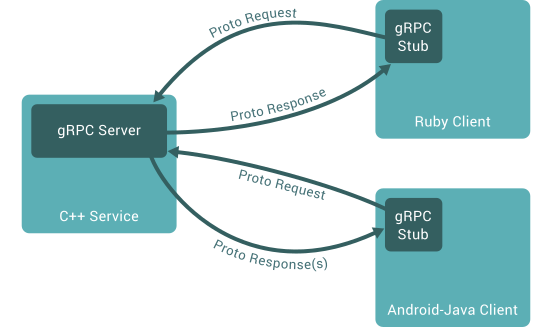
\includegraphics[width=0.6\textwidth]{resources/grpc.png}
      \caption{The architecture of gRPC}
\end{figure}


\subsection{The CSI Remote Procedure Calls}

\begin{figure}[ht]
      \centering
      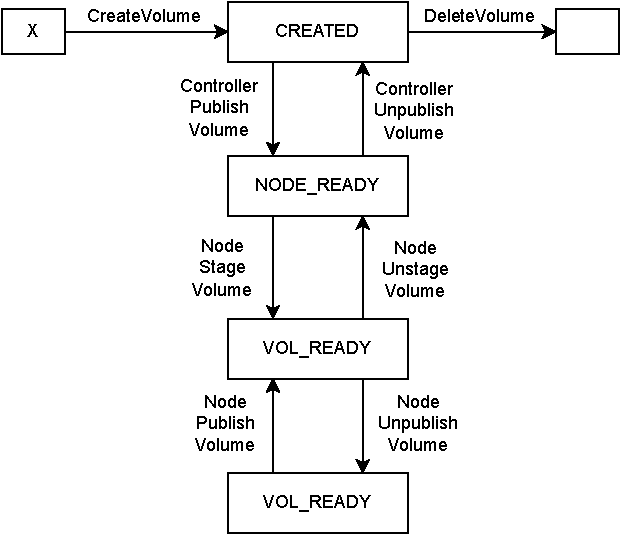
\includegraphics[width=0.7\textwidth]{resources/csi-states.pdf}
      \caption{The lifecycle of a dynamically provisioned volume, from creation
            to destruction.}
      \label{figure:csi-calls}
\end{figure}

The Container Storage Interface defines the RPCs a container orchestrator uses
in order to interact with the storage driver. Each of the RPCs is an idempotent
operation. The order the calls can be issued is show in Figure
\ref{figure:csi-calls}. The list of available RPCs is the following:

\begin{itemize}

      \item{\co{CreateVolume}}: The external provisioner issues this RPC to the
            CSI Controller service, asking it to provision a new volume on
            behalf of a user. If the plugin is unable to complete the
            \co{CreateVolume} call successfully, it must return a non-OK gRPC
            code in the gRPC status.

            Of particular interest in the context of the thesis is the
            \co{RESOURCE\_EXHAUSTED} code; If the controller plugin responds
            with this code, it indicates that it cannot provision the requested
            volume with the specified topology constraints, possibly due to
            insufficient storage capacity.

      \item{\co{ControllerPublishVolume}}: The external attacher issues
            this RPC to the CSI Controller service when Kubernetes wants to
            place a workload that uses the (already provisioned) volume onto a
            node. The plugin should perform the necessary work to make the
            volume available on the given node.

      \item{\co{NodeStageVolume}}:  The kubelet issues this RPC to the  CSI Node
            service when the volume is to be used by the first Pod on the node.
            It should be issued only after \co{NodePublishVolume} has succeeded.
            It is essentially used to format the volume and mount it on a
            staging directory on the node.

      \item{\co{NodePublishVolume}}: The  kubelet issues this RPC to the  CSI
            Node service when a Pod starts to run on a node. It essentially
            mounts the volume to the directory of the Pod.

      \item{\co{NodeUnpublishVolume}}: The kubelet issue this RPC to the CSI
            Node service to undo the work done by the corresponding
            \co{NodePublishVolume}. It essentially unmounts the volume from the
            directory of the Pod.

      \item{\co{NodeUnstageVolume}}: The kubelet issues the RPC to the CSI Node
            service to undo the work by the corresponding \co{NodeStageVolume}.
            It essentially unmounts the volume from the staging directory of the
            node.

      \item{\co{ControllerUnpublishVolume}}: The external attacher issues this
            RPC to the CSI Controller service to perform the work necessary for
            making the volume ready to be consumed by a different node. It
            essentially undoes any work done by the
            \co{ControllerPublishVolume}.

      \item{\co{DeleteVolume}}: The external provisioner issues this RPC to the
            CSI Controller service to deprovision a volume. It is the reverse
            operation of the \co{CreateVolume}.

\end{itemize}


\subsection{Kubernetes CSI Sidecars}
The Kubernetes CSI sidecars containers are a set of standard containers that aim
to simplify the development and deployment of CSI drivers on Kubernetes. These
containers contain common logic to watch the Kubernetes API, trigger appropriate
operations against the \textit{CSI driver} container, and update the Kubernetes
API as appropriate. The containers are intended to be bundled with third-party
CSI driver containers and deployed together as Pods.



\subsubsection{CSI External Provisioner}
\label{csi-external-provisioner}
\label{section:provisioner}

The CSI external provisioner is a sidecar container that watches the Kubernetes
API server for \texttt{PersistentVolumeClaim} objects. If a PVC requests for
dynamic provisioning of a volume and has the selected node annotation
\footnote{Selected node annotation: \co{volume.kubernetes.io/selected-node:
            <node-name>}}, the external provisioner issues a \co{CreateVolume} RPC against
the CSI Controller service to provision a new volume accessible from the
selected node. Suppose the Controller service responds with a
\co{ResourceExhausted} status code. In that case, the external provisioner will
remove the selected node annotation from the PVC, to signal back to the
scheduler that the provisioning of the volume has failed, and it shall retry the
scheduling. Once the external provisioner successfully provisions the volume, it
creates a Kubernetes \texttt{PersistentVolume} object to represent the volume
and binds it to the PVC.

The deletion of a \texttt{PersistentVolumeClaim} object bound to a
\texttt{PersistentVolume} corresponding to this driver with a \texttt{delete}
reclaim policy causes the external provisioner to trigger a
\texttt{DeleteVolume} operation against the CSI Controller service to delete the
volume. Once the volume is successfully deleted, the sidecar container deletes
the \texttt{PersistentVolume} object representing the volume.

\subsubsection{CSI External Attacher}

The CSI external attacher is a sidecar container that watches the Kubernetes API
server for \texttt{VolumeAttachment} objects and triggers
\co{ControllerPublishVolume} and \co{ControllerUnpublishVolume} operations
against a CSI endpoint.


\subsubsection{CSI Node Driver Registrar}

The CSI node driver registrar is a sidecar container that fetches driver
information  by issuing a \texttt{NodeGetInfo}) to the CSI Node service and
registers the driver with the kubelet on that node.  The registration is
necessary because the kubelet is responsible for issuing CSI \co{NodeGetInfo},
\co{NodeStageVolume}, \co{NodePublishVolume} calls. By registering the CSI
driver, the kubelet learns which Unix domain socket to issue the CSI calls on.
\subsection{Kubernetes CSI: An End-to-End Story}

In this section, we aim to combine all the information by describing an
end-to-end story for the CSI.  We present the timeline of actions that take
place under the hood in order to provision a  volume dynamically.

The timeline of actions is the following:

\begin{enumerate}
	\tightlist
	\item The cluster administrator creates a StorageClass (in our case, the
	      \co{Rok} storage class) that specifies the CSI plug-in name
	      (\co{provisioner:rok.arrikto.com}):
	      \lstinputlisting[language=yaml]{code/rok-sc.yaml}

	\item A user creates a PersistentVolumeClaim that requests a volume of at
	      least 10 Gi with access mode \co{ReadWriteOnce} from the \co{Rok}
	      storage class.

	      \lstinputlisting[language=yaml]{code/pvc-rok.yaml}

	      Since the \co{Rok} StorageClass has \co{volumeBindingMode:
		      WaitForFirstConsumer}, the volume for the PVC will not be
	      provisioned as long as a Pod requesting the PVC is not scheduled
	      on a node. he PVC to be provisioned.
	\item  A user creates a Pod that uses the PVC:
	      \lstinputlisting[language=yaml]{code/pod-pvc-rok.yaml}
	\item The VolumeBinding plugin of the scheduler does not find any PV to
	      match the PVC. It signals the driver to provision the volume
	      dynamically: it annotates the PVC with the selected node annotation..
	\item The external provisioner sidecar that runs along with the Rok CSI
	      driver sees the annotation on the PVC and issues a \co{CreateVolume}
	      call against the Rok CSI Controller service to provision the volume.
	\item The Rok CSI controller provisions the volume and returns a successful
	      response to the external provisioner.
	\item The external provisioner creates a \co{PersistentVolume} object on the API
	      Server and binds it (the PV) to the  PVC.
	\item The PersistentVolume controller completes the bidirectional binding of
	      the PV and the PVC (by binding the PVC to the PV).
\end{enumerate}
\section{Logical Volume Management}
\label{section:background-lvm}

Logical Volume Management enables combining multiple individual hard drives and
disk partitions into a single volume group (VG). That volume group can then be
subdivided into logical volumes (LV) or used as a single large volume. Regular
file systems, such as EXT3 or EXT4, can then be created on a logical volume.


Logical volume manager (LVM) introduces an extra layer between the physical
disks and the file system, allowing file systems to:
\begin{itemize}
      \tightlist
      \item
            Be resized and moved with ease and online without requiring a
            system-wide outage.
      \item
            Use discontinuous space on disk.
      \item
            Have meaningful names to volumes, rather than the usual cryptic
            device names.
      \item
            Span multiple physical disks.
\end{itemize}

\begin{figure}[ht]
      \centering
      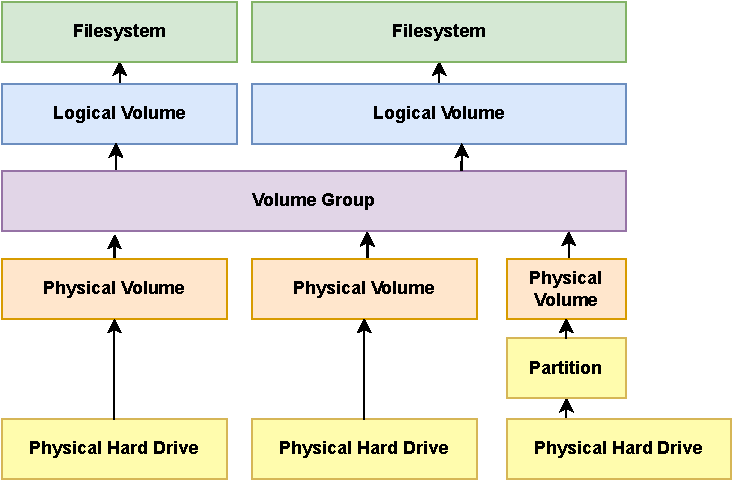
\includegraphics[width=0.8\textwidth]{resources/lvm.pdf}
      \caption{The Logical Volume Management layers}
\end{figure}

The Logical Volume Management consists of the following conceptual layers:
\begin{itemize}
      \item
            \textbf{Physical Volume}: Each Physical Volume can be a disk
            partition, whole disk, meta-device, or a loopback file.
      \item
            \textbf{Volume Group} (VG): A Volume Group gathers a collection of
            Logical Volumes and Physical Volumes into one administrative unit. A
            volume group is divided into fixed-size physical extents. VGs are
            made up of Physical Volumes, which, in turn, are made up of
            physical extents (PEs).

      \item
            \textbf{Logical Volume} (LV): A Logical Volume is the conceptual
            equivalent of a disk partition in a non-LVM system. Logical volumes
            are block devices that are created from the physical extents present
            in the same volume group.
\end{itemize}

\section{Rok's Local Volume Mechanism}

Local data on a node need a mechanism to be backed up if the node gets removed
from the cluster; otherwise, the data will be permanently lost, and the user
will not be able to recover them.

Rok provides a mechanism that enables the functionality of moving volumes around
the nodes of a cluster. It leverages an external storage system, such as
Amazon's S3, where it snapshots the local volumes and can restore them on a
different node. Rok refers to moving a local volume to Amazon S3 as
\textit{``Unpinning''} and restoring the volume to a different node as
\textit{``Pinning''}. We describe this mechanism in greater depth in the
following section.

\subsection{Rok Volume Pinning and Unpinning}

\label{section:rok-volume-pinning}

When a local volume is provisioned on a node, the corresponding
\co{PersistentVolume} object on the API Server that represents the volume has
node affinity on it (see section \ref{section:background-pv-node-affinity}). In
the case of local storage, the Rok CSI driver sets the node affinity of the PV
to match only with the node where the local volume is provisioned.


Rok introduces the following terms:
\begin{itemize}
	\tightlist

	\item \textit{Pinned PV}: A PV representing a node's local volume. This PV
	      has node affinity to indicate that it is accessible only from that
	      particular node.
	\item \textit{Unpinned PV}: A PV representing a local volume migrated to S3.
	      The PV has an empty node affinity to indicate that it is accessible
	      from every cluster node.
\end{itemize}

A pinned PV can become unpinned with the process of ``\textit{unpinning}''. An
unpinned PV can become pinned with the process of ``\textit{pinning}''. The
process can be repeated multiple times, essentially allowing the volume to move
around the cluster nodes as many times as needed.

\label{section:design-unpin}
The Rok CSI Controller implements the following mechanism for the unpinning of a
PV:
\begin{enumerate}
	\tightlist
	\item Watches for nodes that are marked unschedulable.
	\item Finds volumes on the unschedulable node that are not currently used by
	      any Pods.
	\item Starts the unpinning process of the unused PV: it takes snapshots of
	      the volume on Amazon S3.
	\item Removes the node affinity from the PV. Note that the \co{nodeAffinity}
	      field of a PV is immutable, i.e., it is not allowed to change. To
	      overcome this restriction, Rok deletes the PV and instantaneously
	      recreates it.
\end{enumerate}

Rok implements the following mechanism for the pinning of a PV:
\begin{enumerate}
	\tightlist
	\item The Scheduler schedules the Pod that references the unpinned PV
	      (through a PVC).
	\item The Kubernetes \co{attachDetach} controller creates a
	      \co{VolumeAttachment} object to signal the external attacher to attach
	      the volume on the node.
	\item The external attacher sees the VolumeAttachment and issues a
	      \co{ControllerPublishVolume} call to the Rok CSI controller.
	\item The Rok CSI controller creates a logical volume on the Rok VG and
	      restores the data of the PV from the Amazon S3 to the logical volume.
	\item The Rok CSI controller sets the appropriate node affinity on the PV to
	      indicate its only accessible from the node the volume was restored to.
\end{enumerate}


\subsection{Rok's Local Volume Protection Mechanism}
\label{section:background-rok-csi-guard}

The Kubernetes maintenance and upgrade tools rely on the \co{drain} operation
(see \ref{section:cordon-drain}). Essentially, before taking any actions to
remove or upgrade a node in the cluster, the tools drain the node (\co{kubectl
	drain}) in order to mark the node unschedulable and safely evict all the Pods.
The Cluster Autoscaler also uses the drain operation before removing a node.

Rok deploys a mechanism to facilitate the upgrades of a cluster and ensure that
the nodes are not removed before Rok snapshots all their local volumes.

The mechanism leverages Pods with properly configured PodDisruptionBudgets to
block their eviction. It relies on the fact that the drain operation fails as
long as the eviction of a Pod fails. The mechanism works as follows:

\begin{enumerate}
	\tightlist
	\item The Rok Operator creates a \co{Deployment} resource \textit{for each
		      node} in the cluster. The Deployment of each node creates
	      \textit{exactly} one replica Pod with node affinity that matches
	      only the specific node. Rok names these Pods  ``\textit{CSI Guard
		      Pod}'', since they protect the node's local volumes.
	\item The Rok Operator creates a \co{PodDisruptionBudget} object for each
	      Rok CSI Guard Deployment. The PodDisruptionBudget demands at any time
	      to exist at least one Rok CSI Guard Pod of the Deployment. This
	      configuration causes any evictions of the Rok CSI Guard Pod to fail.
	\item The drain operation marks the node unschedulable and starts evicting
	      the Pods on the node. The eviction of the CSI Guard fails because of
	      the configured PodDisruptionBudget.
	\item The Rok Operator checks if the Rok CSI has unpinned all the volumes of
	      the unschedulable node; if this condition holds, it removes the
	      PodDisruptionBudget that corresponds to the CSI Guard of the node.
	\item Since the PodDisruptionBudget does not exist anymore, the eviction of
	      the  Rok CSI Guard Pod finally succeeds, and the drain operation
	      completes.
\end{enumerate}

The mechanism is illustrated in Figure ~\ref{figure:rok-csi-guards}.

\clearpage
\vspace*{2cm}
\begin{figure}[H]
	\centering
	\makebox[\textwidth][c]{
		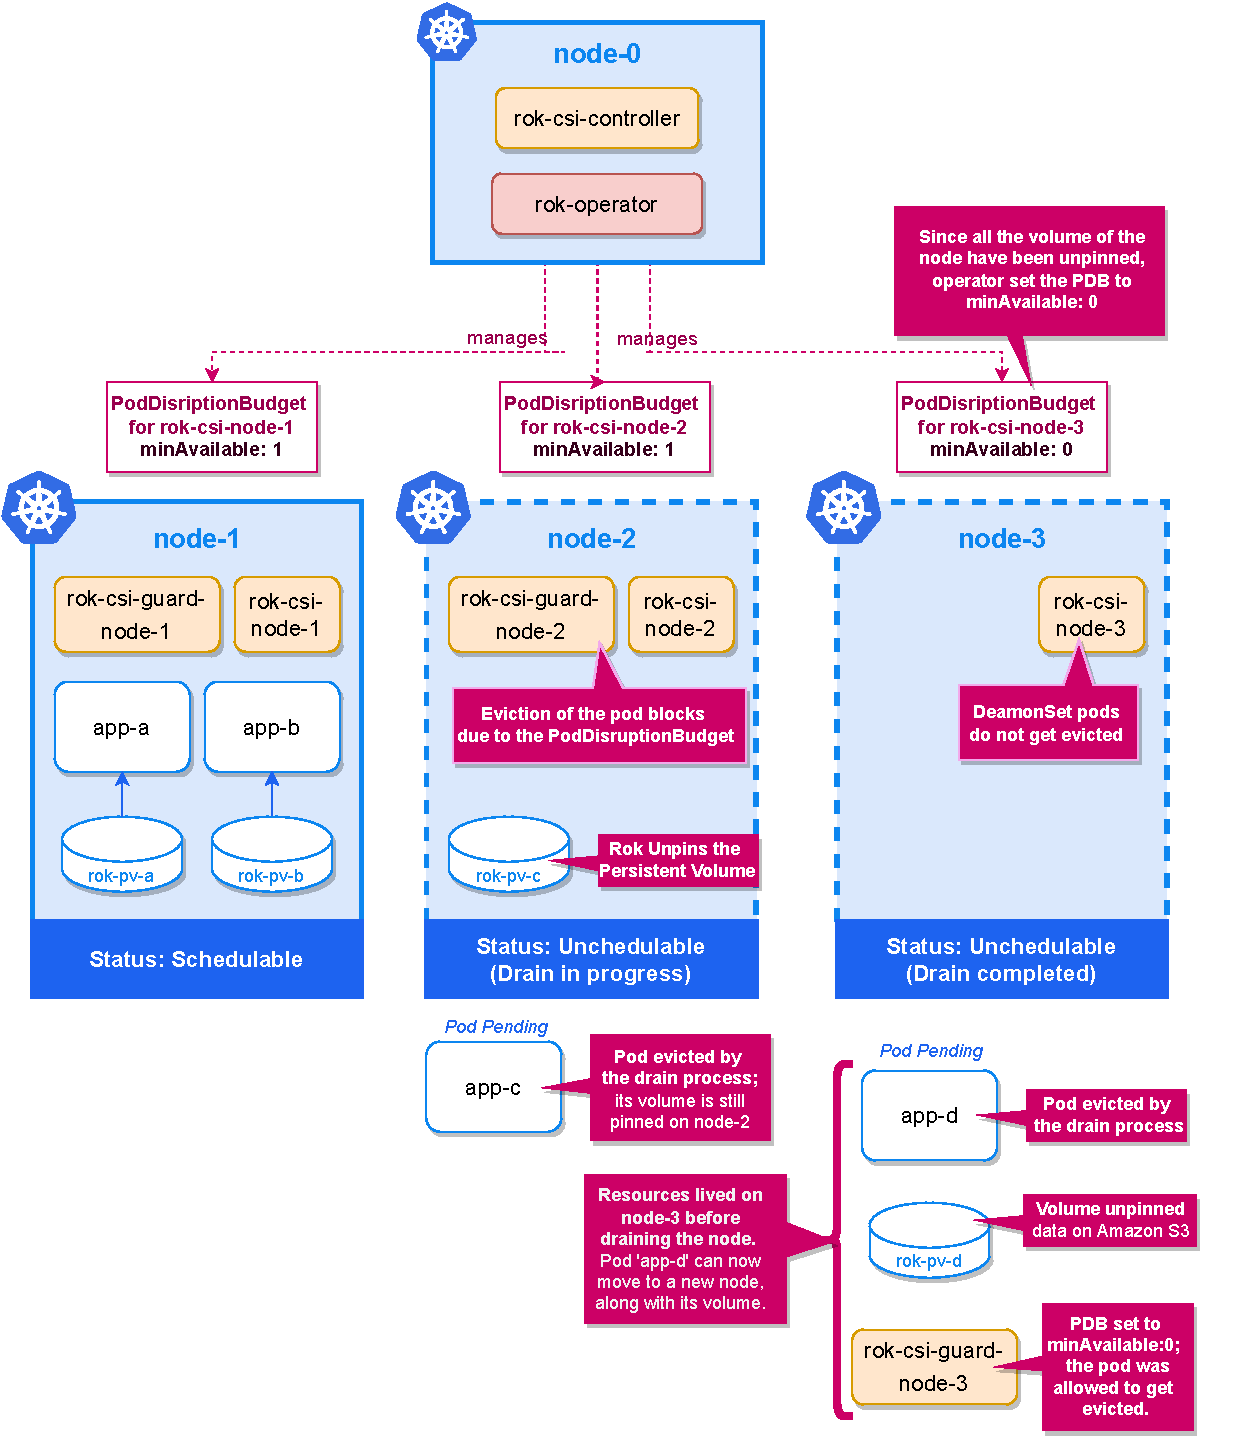
\includegraphics[width=1.2\textwidth]{resources/drain-cluster.pdf}
	}
	\caption{Protecting Local Data with Rok CSI Guard Pods}
	\label{figure:rok-csi-guards}
\end{figure}
\clearpage
\chapter{Design} \label{chapter:design}

In this chapter, we describe the design and algorithms that discipline the
operation of the Cluster Autoscaler and the Scheduler; we point out their
shortcomings concerning local data storage and propose design enhancements to
enable seamless scheduling and autoscaling with local persistent volumes.

\section{Design Rationale \& Goals}

As explained in section \ref{section:intro_problem_statement}, our goal is to
extend the Scheduler and the Cluster Autoscaler so that they operate seamlessly
with workloads that use volumes backed by local storage. More specifically, we
aim to:

\begin{itemize}
      \tightlist
      \item Extend the Scheduler to consider the storage capacity of the nodes
            when scheduling Pods.
      \item Extend the Autoscaler to scale-down nodes where local volumes live,
            ensuring that Rok's mechanism snapshots the data before removing the
            node from the cluster.
      \item Extend the Autoscaler to check if the Pod's volumes can be placed on
            any other node (with regards to storage capacity) when evaluating (for
            a possible scale-down) if a Pod can be moved elsewhere.
      \item Extend the Autoscaler to consider the storage capacity of nodes, and,
            when scaling up, add a node with enough storage capacity.
      \item Extend the Autoscaler to not remove unready nodes in case local
            volumes live on these nodes.
\end{itemize}

\section{Rok's Local Volume Mechanism}

Local data on a node need a mechanism to be backed up if the node gets removed
from the cluster; otherwise, the data will be permanently lost, and the user
will not be able to recover them.

Rok provides a mechanism that enables the functionality of moving volumes around
the nodes of a cluster. It leverages an external storage system, such as
Amazon's S3, where it snapshots the local volumes and can restore them on a
different node. Rok refers to moving a local volume to Amazon S3 as
\textit{``Unpinning''} and restoring the volume to a different node as
\textit{``Pinning''}. We describe this mechanism in greater depth in the
following section.

\subsection{Rok Volume Pinning and Unpinning}

\label{section:rok-volume-pinning}

When a local volume is provisioned on a node, the corresponding
\co{PersistentVolume} object on the API Server that represents the volume has
node affinity on it (see section \ref{section:background-pv-node-affinity}). In
the case of local storage, the Rok CSI driver sets the node affinity of the PV
to match only with the node where the local volume is provisioned.


Rok introduces the following terms:
\begin{itemize}
	\tightlist

	\item \textit{Pinned PV}: A PV representing a node's local volume. This PV
	      has node affinity to indicate that it is accessible only from that
	      particular node.
	\item \textit{Unpinned PV}: A PV representing a local volume migrated to S3.
	      The PV has an empty node affinity to indicate that it is accessible
	      from every cluster node.
\end{itemize}

A pinned PV can become unpinned with the process of ``\textit{unpinning}''. An
unpinned PV can become pinned with the process of ``\textit{pinning}''. The
process can be repeated multiple times, essentially allowing the volume to move
around the cluster nodes as many times as needed.

\label{section:design-unpin}
The Rok CSI Controller implements the following mechanism for the unpinning of a
PV:
\begin{enumerate}
	\tightlist
	\item Watches for nodes that are marked unschedulable.
	\item Finds volumes on the unschedulable node that are not currently used by
	      any Pods.
	\item Starts the unpinning process of the unused PV: it takes snapshots of
	      the volume on Amazon S3.
	\item Removes the node affinity from the PV. Note that the \co{nodeAffinity}
	      field of a PV is immutable, i.e., it is not allowed to change. To
	      overcome this restriction, Rok deletes the PV and instantaneously
	      recreates it.
\end{enumerate}

Rok implements the following mechanism for the pinning of a PV:
\begin{enumerate}
	\tightlist
	\item The Scheduler schedules the Pod that references the unpinned PV
	      (through a PVC).
	\item The Kubernetes \co{attachDetach} controller creates a
	      \co{VolumeAttachment} object to signal the external attacher to attach
	      the volume on the node.
	\item The external attacher sees the VolumeAttachment and issues a
	      \co{ControllerPublishVolume} call to the Rok CSI controller.
	\item The Rok CSI controller creates a logical volume on the Rok VG and
	      restores the data of the PV from the Amazon S3 to the logical volume.
	\item The Rok CSI controller sets the appropriate node affinity on the PV to
	      indicate its only accessible from the node the volume was restored to.
\end{enumerate}


\subsection{Rok's Local Volume Protection Mechanism}
\label{section:background-rok-csi-guard}

The Kubernetes maintenance and upgrade tools rely on the \co{drain} operation
(see \ref{section:cordon-drain}). Essentially, before taking any actions to
remove or upgrade a node in the cluster, the tools drain the node (\co{kubectl
	drain}) in order to mark the node unschedulable and safely evict all the Pods.
The Cluster Autoscaler also uses the drain operation before removing a node.

Rok deploys a mechanism to facilitate the upgrades of a cluster and ensure that
the nodes are not removed before Rok snapshots all their local volumes.

The mechanism leverages Pods with properly configured PodDisruptionBudgets to
block their eviction. It relies on the fact that the drain operation fails as
long as the eviction of a Pod fails. The mechanism works as follows:

\begin{enumerate}
	\tightlist
	\item The Rok Operator creates a \co{Deployment} resource \textit{for each
		      node} in the cluster. The Deployment of each node creates
	      \textit{exactly} one replica Pod with node affinity that matches
	      only the specific node. Rok names these Pods  ``\textit{CSI Guard
		      Pod}'', since they protect the node's local volumes.
	\item The Rok Operator creates a \co{PodDisruptionBudget} object for each
	      Rok CSI Guard Deployment. The PodDisruptionBudget demands at any time
	      to exist at least one Rok CSI Guard Pod of the Deployment. This
	      configuration causes any evictions of the Rok CSI Guard Pod to fail.
	\item The drain operation marks the node unschedulable and starts evicting
	      the Pods on the node. The eviction of the CSI Guard fails because of
	      the configured PodDisruptionBudget.
	\item The Rok Operator checks if the Rok CSI has unpinned all the volumes of
	      the unschedulable node; if this condition holds, it removes the
	      PodDisruptionBudget that corresponds to the CSI Guard of the node.
	\item Since the PodDisruptionBudget does not exist anymore, the eviction of
	      the  Rok CSI Guard Pod finally succeeds, and the drain operation
	      completes.
\end{enumerate}

The mechanism is illustrated in Figure ~\ref{figure:rok-csi-guards}.

\clearpage
\vspace*{2cm}
\begin{figure}[H]
	\centering
	\makebox[\textwidth][c]{
		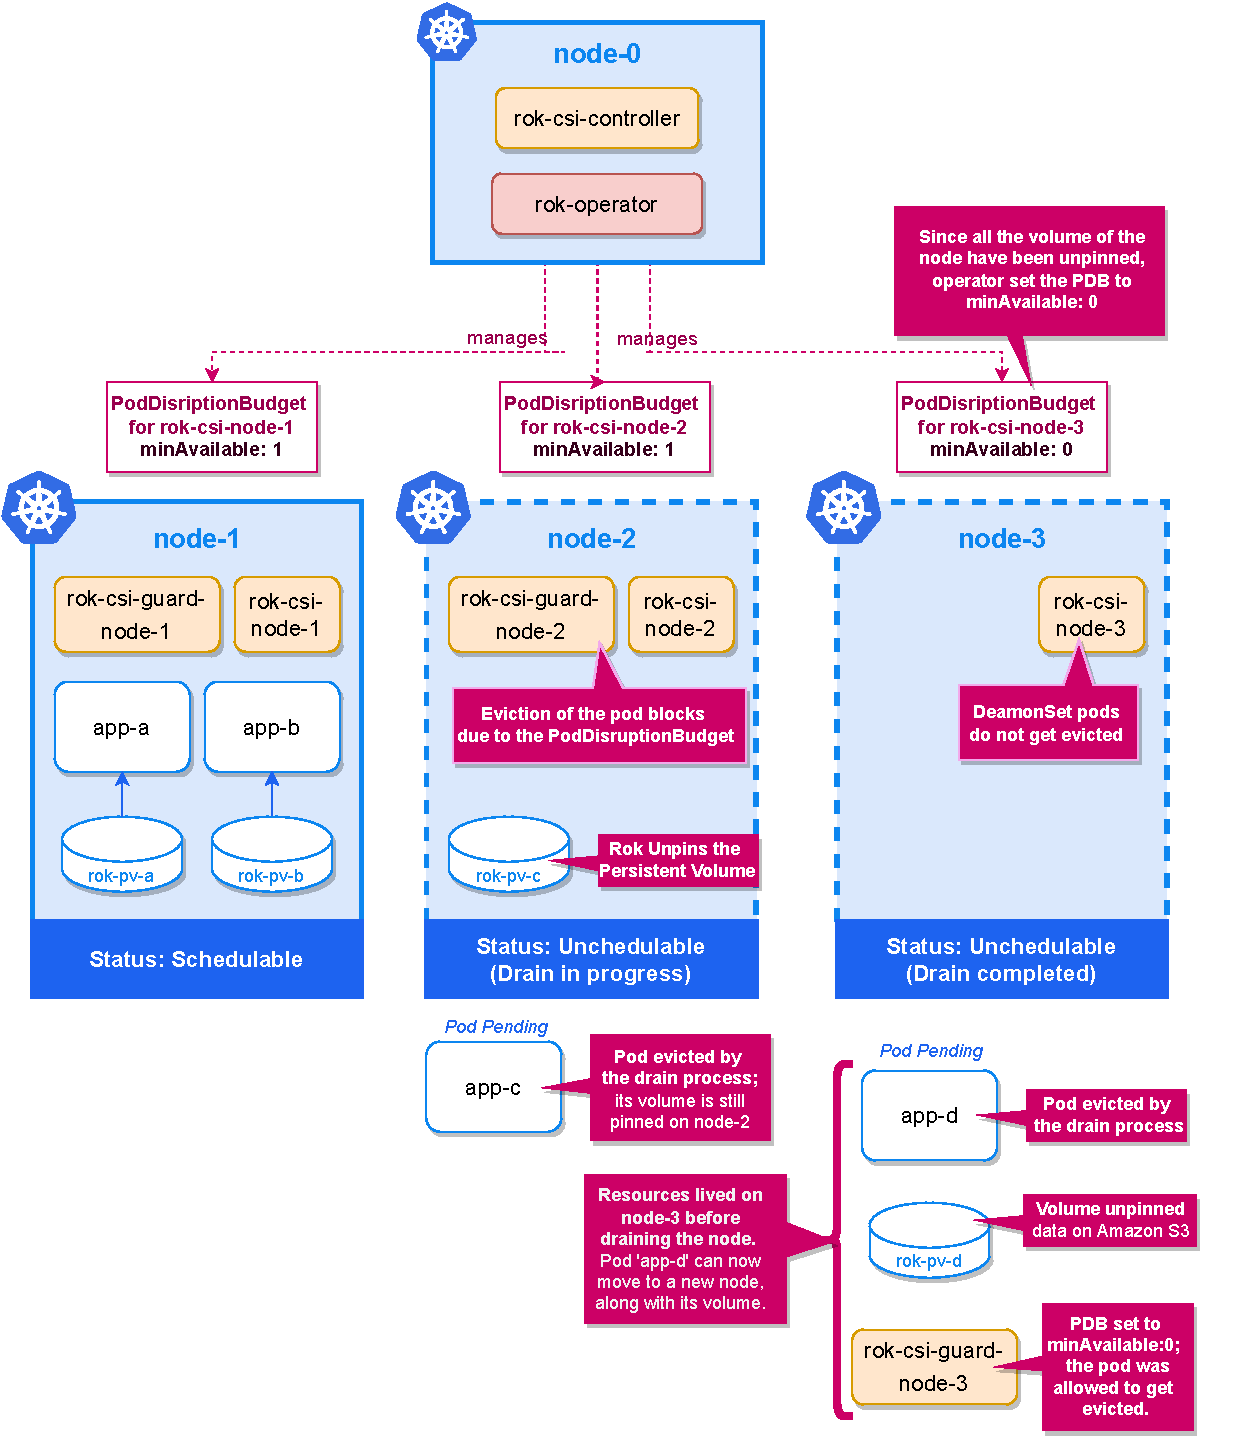
\includegraphics[width=1.2\textwidth]{resources/drain-cluster.pdf}
	}
	\caption{Protecting Local Data with Rok CSI Guard Pods}
	\label{figure:rok-csi-guards}
\end{figure}
\clearpage
\section{Kubernetes Scheduler}
\RestyleAlgo{ruled}

Σε αυτήν την ενότητα, θα παρουσιάσουμε συνοπτικά τη τρέχουσα σχεδίαση του
Kubernetes Scheduler, θα επισημάνουμε τις ελλείψεις που υπάρχουν και θα
προτείνουμε βελτιώσεις που επιλύουν τους τρέχοντες περιορισμούς.

\subsection{To Πρόσθετο VolumeBinding}

Για λόγους συντομίας, στο ελληνικό τμήμα της διπλωματικής παρουσιάζουμε μόνο τη
σχεδίαση της \co{Filter} και της \co{PreBind}  φάσης του προσθέτου, καθώς
σχετίζεται άμεσα με τις προτεινόμενες επεκτάσεις. Για την αναλυτική παρουσίαση
των υπολοίπων φάσεων του προσθέτου, μπορείτε να ανατρέξετε στο αντίστοιχο
αγγλικό κεφάλαιο, στην ενότητα \ref{section:design-volume-binding}.

\subsection*{PreFilter Φάση}

\co{Filter}: αξιολογεί αν ένα Pod μπορεί να τοποθετηθεί σε έναν κόμβο, βάσει των
τόμων που ζητά, τόσο για τα δεσμευμένα όσο και για τα μη δεσμευμένα PVC:
\begin{itemize}
      \tightlist
      \item Για τα \textit{δεσμευμένα PVC}, ελέγχει ότι το PV του κάθε PVC είναι
            προσβάσιμο (βάσει τoy node affinity που φέρει) από τον εξεταζόμενο
            κόμβο.
      \item Για τα \textit{μη δεσμευμένα PVC}, προσπαθεί να βρει διαθέσιμα PVs
            που μπορούν να ικανοποιήσουν τις απαιτήσεις του PVC και που είναι
            προσβάσιμα (βάσει του node affinity τους) από τον εξεταζόμενο κόμβο.
            Τα PVCs για τα οποία δεν κατάφερε να βρει κατάλληλα PVs, θα τα
            αποκαλούμε εφεξής ``\textit{PVCs to provision}''.
      \item Για κάθε \textit{PVC to provision}, ελέγχει αν η \co{StorageClass}
            του PVC υποστηρίζει τη δυναμική παροχή και αν υπάρχει αρκετή
            χωρητικότητα αποθήκευσης προσβάσιμη από τον κόμβο. Εάν όχι, το Pod
            δεν μπορεί να ανατεθεί στον κόμβο. Αυτό είναι το βήμα όπου
            η χωρητικότητα αποθήκευσης λαμβάνεται υπόψη.

\end{itemize}

Η τρέχουσα υλοποίηση του χρονοδρομολογητή, ελέγχει αν υπάρχει αρκετή
χωρητικότητα για κάθε PVC to provision, καλώντας τη μέθοδο \co{hasEnough()} με
ένα μόνο PVC ως είσοδο. Ζητά από τον  API Server όλα τα αντικείμενα
\co{CSIStorageCapacity}. και ελέγχει αν κάποιο από αυτά ταιριάζει με το
\co{StorageClass} του PVC, είναι προσβάσιμο από τον εξεταζόμενο κόμβο και η
αναφερόμενη χωρητικότητα του αντικειμένου είναι μεγαλύτερη από τη ζητούμενη
χωρητικότητα του PVC. Εάν ένα τέτοιο CSIStorageCapacity υπάρχει, υπάρχει αρκετός
χώρος στον κόμβο για τη δυναμική παροχή τόμου για το εξεταζόμενο PVC.

Είναι σημαντικό να επισημάνουμε ότι δεν ελεγχει αν υπάρχει αποθηκευτικός χώρος
συνολικά για όλα τα PVCs, αλλά μόνο αν το κάθε PVC χωριστά χωράει σε έναν κόμβο.

\subsection*{PreBind Φάση}

Η φάση \co{PreBind} εκτελείται αφού ο χρονοδρομολογητής έχει επιλέξει έναν κόμβο
για  το Pod.

Για κάθε ένα από τα \textit{μη δεσμευμένα PVC} που το πρόσθετο βρήκε ένα
κατάλληλο PV κατά τη διάρκεια της φάσης \co{Filter}, θα ενημερώσει τον API
Server με τη δέσμευση, δηλαδή, θα ενημερώσει το αντίστοιχο PV ώστε να δείχνει
στο PVC, και στη συνέχεια, ο ελεγκτής Kubernetes PersistentVolume θα ολοκληρώσει
την αμφίδρομη δέσμευση.

Για κάθε ένα από τα \textit{PVCs to provision}, θα ενημερώσει τα αντίστοιχα PVCs
στον API Server με το  ``selected node annotation'' \footnote{Το selected node
annotation: \co{volume.kubernetes.io/selected-node}} για να σηματοδοτήσει στον
\en{external provisioner} ότι ένας τόμος για το PVC πρέπει να δημιουργηθεί δυναμικά
σε ένα τμήμα τοπολογίας που είναι προσβάσιμο από τον κόμβο που υποδεικνύει η
σημείωση. 

Στη συνέχεια, το πρόσθετο θα κάνει poll τον API Server έως ότου όλα τα PVCs
δεσμευτούν  PVs. Εάν το selected node annotation κάποιου PVC to provision
αφαιρεθεί, θα ακυρώσει την τρέχουσα προσπάθεια χρονοδρομολόγησης και θα
καλέσει τα πρόσθετα \co{Unreserve}.Η αφαίρεση του annotation είναι ένας
μηχανισμός με τον οποίο ο external provisioner ουσιαστικά ειδοποιεί τον
χρονοδρομολογητή ότι απέτυχε η παροχή του τόμου και θα πρέπει να δοκιμάσει ξανά,
ενδεχομένως σε άλλον κόμβο.


\subsection{Ελλείψεις \& Προτεινόμενες Επεκτάσεις}

Σύμφωνα με την προηγούμενη ανάλυση των αλγορίθμων, ο τρέχων σχεδιασμός του
Kubernetes Scheduler έχει τους ακόλουθους περιορισμούς:

\begin{enumerate}
      \item Η μέθοδος \texttt{Filter} του πρόσθετου VolumeBinding χρησιμοποιεί
            τα αντικείμενα \en{CSIStorageCapacity} του Kubernetes API για να
            αντλήσει πληροφορίες για τον διαθέσιμο αποθηκευτικό χώρο. Αυτό το
            αντικείμενο API έγινε beta στην έκδοση Kubernetes 1.21 και ήταν σε
            κατάσταση alpha σε προηγούμενες εκδόσεις. Οι κύριοι πάροχοι
            υπηρεσιών νέφους δεν ενεργοποιούν τα χαρακτηριστικά σε κατάσταση
            alpha στις υπηρεσίες τους. Ως αποτέλεσμα, τα CSIStorageCapacity
            αντικείμενα δεν είναι ενεργοποιημένα σε συστοιχίες που εκτελούν
            εκδόσεις προγενέστερες της 1.21 στους περισσότερους παρόχους cloud.
            Αυτό είναι ένα σημαντικό πρόβλημα, δεδομένου ότι πολλές επιχειρήσεις
            (συμπεριλαμβανομένων των πελατών μας) δεν τρέχουν τις τελευταίες
            εκδόσεις του Kubernetes για λόγους σταθερότητας. Στη δική μας
            περίπτωση, οι πελάτες μας εκτελούν συστοιχίες Kubernetes 1.19 και
            1.20 και χρειάζονταν τη δυνατότητα χρονοδρομολόγησης Pods με εξέταση
            της τοπικής αποθήκευσης.
      \item Η τρέχουσα σχεδιαστική λογική της φάσης \co{Filter} του πρόσθετου
            \co{VolumeBinding} δεν λαμβάνει υπόψη της τον αποθηκευτικό χώρο που
            απαιτείται για την παροχή πολλαπλών PVC ενός Pod. Αντ' αυτού,
            ελέγχει αν κάθε μεμονωμένο PVC μπορεί να δημιουργηθεί στον
            αποθηκευτικό χώρο που είναι προσβάσιμος από τον κόμβο, χωρίς να
            διασφαλίζει ότι υπάρχει αρκετός χώρος για όλα αυτά ταυτόχρονα. Αυτό
            είναι ένα κρίσιμο πρόβλημα: σε περίπτωση που ένα Pod αναφέρεται σε
            πολλαπλά μη δεσμευμένα PVC και δεν υπάρχει αρκετός χώρος για όλα
            αυτά, ένα από αυτά γίνει provision και η παροχή των υπολοίπων θα
            αποτύχει, τότε όλες οι μελλοντικές αποφάσεις χρονοδρομολόγησης θα
            περιορίζονται από το ήδη δημιουργημένο τόμο και το Pod θα κολλήσει.
\end{enumerate}

Δεδομένου ότι ο σχεδιασμός του upstream έρχεται με τους προαναφερθέντες
περιορισμούς, προτείνουμε να επεκτείνουμε τον Kubernetes Scheduler και να
εγκαταστήσουμε τον επεκταμένο χρονοδρομολογητή στη συστοιχία. Ο προτεινόμενος
σχεδιασμός μπορεί να χωριστεί στα ακόλουθα μέρη:

% TODO: enumerate or itemize?
\begin{enumerate}
      \tightlist
      \item Επέκταση του Rok CSI Node του οδηγού αποθήκευσης, ώστε να
            αναφέρει τη διαθέσιμη χωρητικότητα κάθε κόμβου ως annotation στο
            αντίστοιχο αντικείμενο \texttt{Node} του Kubernetes.
      \item Επέκταση του Rok CSI Controller του οδηγού αποθήκευσης
            ώστε να απαντά με κατάλληλο σφάλμα στην κλήση \co{CreateVolume} όταν
            η εναπομένουσα χωρητικότητα για την παροχή του τόμου είναι
            ανεπαρκής.
      \item Επέκταση του πρόσθετου VolumeBinding του Kubernetes Scheduler ώστε
            να ελέγχει αν πολλαπλοί τόμοι ενός Pod χωρούν σε έναν κόμβο,
            συγκρίνοντας τη συνολική τους απαίτηση σε χωρητικότητα με την
            αναφερθείσα διαθέσιμη χωρητικότητα.
      \item Εγκατάσταση του επεκταμένου χρονοδρομολογητή στη συστοιχία.
      \item Ανάπτυξη και εγκατάσταση ενός  webhook που θα μεταλλάσσει τα Pods
            ώστε να χρησιμοποιούν τον επεκταμένο χρονοδρομολογητή.
\end{enumerate}

\subsubsection{Επέκταση του Rok CSI Node}

Δεδομένου ότι τα αντικείμενα \co{CSIStorageCapacity} δεν μπορούν να γίνουν
back-port σε προηγούμενες εκδόσεις του Kubernetes και, επίσης, η προσθήκη ενός
παρόμοιου Custom Resource θα απαιτούσε αρκετή προσπάθεια άνευ αιτίας,
αποφασίζουμε να αναφέρουμε τη χωρητικότητα κάθε κόμβου ως annotation στο
αντίστοιχο αντικείμενο Node. Το annotation, το οποίο αποκαλούμε ``annotation
χωρητικότητας'' θα είναι της μορφής
\co{rok.arrikto.com/capacity:<free-storage-bytes>}.

Το πρόσθετο Rok CSI Node του οδηγού αποθήκευσης που εκτελείται σε κάθε κόμβο της
συστοιχίας υπολογίζει περιοδικά τον διαθέσιμο αποθηκευτικό χώρο και ενημερώνει
το annotation χωρητικότητας. Δίνει εντολές στο Logical Volume Manager (LVM) του
κόμβου για να μάθει τον ελεύθερο χώρο του Rok Volume Group και ενημερώνει το
αντίστοιχο \co{Node} αντικείμενο με την τιμή της διαθέσιμης χωρητικότητας.

\subsubsection{Επέκταση του Rok CSI Controler}

Επεκτείνουμε το πρόσθετο Rok CSI Controller του οδηγού αποθήκευσης ώστε να
επιστρέφει το status  code \co{GRPCResourceExhausted} ως απάντηση στην κλήση
\co{CreateVolume} του external provisioner όταν η παροχή ενός τόμου αποτυγχάνει
λόγω ανεπαρκούς χωρητικότητας αποθήκευσης.

\subsubsection{Επέκταση του VolumeBinding Plugin}
\label{section:gr-volume-plugin-extensions}

Προτείνουμε την επέκταση της \co{Filter} μεθόδου του πρόσθετου
\co{VolumeBidning} ως εξής:
\begin{enumerate}
      \tightlist
      \item Κατά τον έλεγχο των PVCs του Pod που χρειάζονται να δημιουργηθούν
            δυναμικά (provision) (μέθοδος \co{checkVolumeProvisions()}), να
            επιλέγει όλα τα Rok PVCs
            \footnote{PVCs provisioned by the \co{rok.arrikto.com}
                  provisioner.} (εφεξής αναφέρονται ως ``\\textit{Rok claims to
                  provision}'') και να ελέγχει αν υπάρχει αρκετή χωρητικότητα
                  για το συνολικό αποθηκευτικό χώρο που ζητούν.
      \item Να ελέγχει αν υπάρχει αρκετή χωρητικότητα για τα Rok claims to
            provision ως εξής:
            \begin{enumerate}
                  \tightlist
                  \item Να υπολογίζει τη συνολική χωρητικότητα που ζητείται
                        αθροίζοντας τα αιτήματά τους.
                  \item Να ελέγχει  αν ο εξεταζόμενος κόμβος διαθέτει annotation
                        χωρητικότητας του Rok \footnote{Το annotation
                        χωρητικότητας του Rok:
                        \texttt{rok.arrikto.com/capacity}} .
                  \item Αν to annotation \textit{δεν υπάρχει}, ή αν υπάρχει αλλά
                        δεν είναι έγκυρος ακέραιος αριθμός, τα Rok claims to
                        provision δεν μπορούν να δημιουργηθούν στον κόμβο. Η
                        απουσία της σημείωσης υποδεικνύει ότι το πρόγραμμα
                        οδήγησης Rok CSI δεν εκτελείται στον κόμβο.
                  \item Εάν υπάρχει το annotation χωρητικότητας, να ελέγχει αν η
                        αναφερόμενη διαθέσιμη χωρητικότητα είναι μεγαλύτερη ή
                        ίση με τη συνολική χωρητικότητα που ζητούν τα Rok claims
                        to provision. Εάν δεν ισχύει η συνθήκη, δεν υπάρχει
                        αρκετή χωρητικότητα, και τα Rok claims to provision δεν
                        μπορούν να δημιουργηθούν στον κόμβο,  οπότε και το Pod
                        δεν μπορεί να προγραμματιστεί στον κόμβο.
            \end{enumerate}
      \item Διατηρούμε της συμβατότητα προς τα πίσω με τη μη τροποποίηση του
            χειρισμού των  PVCs που δεν ζητούν αποθηκευτικό χώρο από την κλάση
            αποθήκευσης Rok. Ο σχεδιασμός μας, διαχωρίζει τα PVCs σε τοπικά Rok
            PVCs και μη Rok PVCs, και επεκτείνει μονάχα τον τρόπο χειρισμού
            μονάχα για τα Rok PVCs. Τα PVC που παρέχονται από άλλους παρόχους
            αποθήκευσης δεν θα επηρεαστούν από τις αλλαγές μας.
\end{enumerate}

% transl: επιπεδο ελέγχου


\subsubsection{Εγκατάσταση του Rok Scheduler}

Ο \co{kube-cheduler} εκτελείται από προεπιλογή σε κάθε πάροχο νέφους ως μέρος
του επιπέδου ελέγχου του Kubernetes και είναι ο προεπιλεγμένος χρονοδρομολογητής
που χρησιμοποιείται για τη χρονοδρομολόγηση των Pods. Οι πάροχοι νέφους
αποκρύπτουν το επίπεδο ελέγχου από τον τελικό χρήστη των υπηρεσιών τους, οπότε
δεν υπάρχει δυνατότητα αντικατάστασης και παραμετροποίησης του εκτελούμενου
χρονοδρομολογητή.

Ως συνέπεια αυτού του περιορισμού, εγκαθιστούμε στη συστοιχία --παράλληλα με τον
προεπιλεγμένο χρονοδρομολογητή--  τον δικό μας χρονοδρομολογητή, που εκτελεί το
επεκταμένο  VolumeBinding πρόσθετο.  Εφεξής θα αναφερόμαστε στον δικό μας
επεκταμένο χρονοδρομολογητή ως ``\textit{Rok Scheduler}''.

\subsubsection{Εγκατάσταση του Rok Scheduler Webhook}

Δεδομένου ότι εγκαθιστούμε τον Rok Scheduler χωρίς να αντικαταστήσουμε το
προεπιλεγμένο Kubernetes Scheduler της συστοιχίας, κάθε Pod πρέπει να καθορίζει
ποιος scheduler θα το χρονοδρομολογήσει ορίζοντας το πεδίο
\co{spec.schedulerName}. Εάν το πεδίο δεν έχει οριστεί, ο προεπιλεγμένος
χρονοδρομολογητής χρησιμοποιείται.

Σίγουρα δεν θέλουμε κάθε χρήστης να ορίζει χειροκίνητα το όνομα του scheduler
στο το Pod - αυτό θα επέτρεπε στους χρήστες να παρακάμψουν την πολιτική
χρονοδρομολόγησης που έχουμε ορίσει, είναι επιρρεπές σε σφάλματα και είναι μια
κουραστική διαδικασία. Χρειαζόμαστε έναν αυτόματο τρόπο για να το πετύχουμε
αυτό. Η λύση για την αυτοματοποίηση της εργασίας, είναι ένα mutating webhook.

Εγκαθιστούμε ένα μεταλλασσόμενο webhook στη συστοιχία, το οποίο στο εξής θα
αναφέρεται ως ``\textit{Rok Scheduler webhook}'', το οποίο δέχεται τα πρόσφατα
δημιουργηθέντα Pods σε συγκεκριμένα namespaces της συστοιχίας και τα
μεταλλάσσει προσθέτοντας το όνομα του Rok Scheduler στο πεδίο
\co{spec.schedulerName}.
\section{Kubernetes Cluster Autoscaler}
\label{section:autoscaler}
\RestyleAlgo{ruled0}

In this section, we are going to expose the design of the Cluster Autoscaler
(Autoscaler), describe its main principles of operation, identify its
limitations and propose extensions that will enable its seamless operation with
local persistent volumes.


\subsection{Fundamental terms}

Before we describe the algorithms of operations of the Autoscaler, it is
essential to understand some fundamental structures and terminology it uses.

\subsubsection{The Node Group Abstraction}

The Autoscaler uses the abstraction of a ``\textit{node group}''. A node group
is not an actual Kubernetes resource but rather an abstraction for a group of
nodes within a cluster. The Autoscaler expects that nodes found within a single
node group have the same resources (CPU, memory, storage) and share several
common properties such as labels and taints. However, they can still
differentiate in some details, e.g., they may consist of more than one
availability zone.

Each node group has the following important properties:
\begin{itemize}
      \tightlist
      \item \co{minSize}:minimum size of the node group.
      \item  \co{maxSize}: maximum size of the node group.
      \item  \co{targetSize}: the target size of the node group.
\end{itemize}

% TODO: Diagram TODO: PVC PV term TODO: All figures dots or not

\subsubsection{The \texttt{CloudProvider} Interface}

The Autoscaler operates with various cloud providers, e.g., GCE, AWS. To achieve
this, it specifies two important interfaces that each cloud provider that aims
to integrate its services with the Autoscaler must implement:
\begin{itemize}
      \tightlist
      \item The \co{CloudProvider} interface:  it contains configuration info
            and functions for interacting with the cloud provider.
      \item The \co{NodeGroup} interface: it contains configuration info and
            functions to control a node group.
\end{itemize}

The \co{NodeGroup} interface builds upon the node group abstraction. Each cloud
provider may choose its interpretation of what is a node group on its service,
as long as it conforms with the abstraction's definition.

For example, in the case of AWS EKS, the implementation of the \co{NodeGroup}
interface maps each node group to an AWS Auto Scaling Group (ASG). An Auto
Scaling group contains a collection of Amazon EC2 instances that are treated as
a logical grouping for automatic scaling and management purposes. An EC2
instance is a virtual server in Amazon Web Services terminology. A cluster
administrator configures the Auto Scaling groups of the EKS cluster and sets
their \co{minSize}, \co{maxSize} accordingly. The Autoscaler interacts with the
AWS cloud provider through the \co{CloudProvider} interface, which (the
CloudProvider interface) lists the configured Auto Scaling groups and maps each
of them to a node group. Only the \co{CloudProvider} interface knows about ASGs;
the rest components of the Autoscaler are unaware of the underlying
implementation and only see node groups.


\subsubsection{The \texttt{ClusterSnapshot} Interface}

The Autoscaler runs simulations on the cluster to make decisions. It takes a
snapshot of the current cluster, adds or removes nodes in the snapshot, and
simulates the scheduling decisions on the modified snapshot. A cluster snapshot
contains a fixed view of the cluster's nodes and the Pods that run on each node.
The \co{ClusterSnapshot} interface describes methods for taking a snapshot of
the cluster nodes and their Pods.

Note that the cluster's PVCs and PVs are not contained in the snapshot. Instead,
they are fetched from the API Server by the VolumeBinding plugin when the
\co{PredicateChecker} checks if a Pod can be placed on a node. We will explain
more about this later on.

\subsubsection{The \texttt{PredicateChecker} interface}

The Autoscaler defines the \co{PredicateChecker} interface, which offers methods
to check whether all required predicates pass for a given Pod and node.

A Predicate is equivalent to a \co{Filter} plugin (see section
\ref{section:background_scheduling_framework}) and it is used to filter out
nodes that can not run a Pod.

These are the methods of the interface:
\begin{itemize}
      \tightlist
      \item \co{CheckPredicates()}: checks if the given Pod can be placed on the
            given node.
      \item \co{FitsAnyNode()}: checks if the given Pod can be placed on any of
            the given nodes.
      \item \co{FitsAnyNodeMatching()}: checks if the given Pod can be placed on
            any of the given nodes matching the provided function.
\end{itemize}


The Autoscaler implements this interface. The implementation is called
\co{SchedulerBasedPredicateChecker} and leverages the Kubernetes Scheduler code.
In particular, the Autoscaler imports the code of the Kubernetes Scheduler and
constructs a list of predicates from the \co{Filter} plugins of the Scheduler.
The Autoscaler uses the \co{SchedulerBasedPredicateChecker} in its simulations
to determine whether a Pod can be placed on a node or not. The methods of the
interface it implements follow this basic flow:
\begin{enumerate}
      \tightlist
      \item Create a new scheduler \co{CycleState}.
      \item Run the \co{preFilter} method of all the plugins. Note that in the
            case of the VolumeBinding plugin, this step fetches the PVCs and PVs
            of the Pod from the API Server and stores them in the
            \co{CycleState}.
      \item Runs all the \co{Filter} plugins to determine if the Pod can be
            placed on the node.
\end{enumerate}

At this point, we shall highlight the fact that the Autoscaler imports the code
of the Kubernetes Scheduler and uses the \co{Filter} plugins it provides in the
\co{SchedulerBasedPredicateChecker} to run a simulation. However, it
\textbf{never} interacts with the live instance of the Kubernetes Scheduler that
runs on the cluster.

\subsubsection{The \texttt{Estimator} \& \texttt{Strategy} Interfaces}

The Autoscaler specifies two interfaces that are used in the scale-up procedure:
\begin{itemize}
      \tightlist
      \item \co{Estimator}: interface for calculating the number of nodes of a
            given type needed to schedule Pods.
      \item \co{Strategy}: interface for selecting the best option to scale up.
\end{itemize}


The estimator currently used by the Autoscaler is \co{BinPackingNodeEstimator}.
This estimator implements the First Fit Decreasing bin packing approximation
algorithm.

%TODO: Bin packing

\subsubsection{Template Nodes}
\label{section:design-template}

As we have explained, the Autoscaler assumes that every node in a node group
will have the same resources (CPU, memory, storage) and labels. It constructs a
template node for each node group to add it to the cluster snapshot and run its
simulations. As the name suggests, a template node represents the details of a
new node of the given node group. A template node is a \co{NodeInfo} struct and
contains the details of a real \co{Node} object and information about the DaemonSet
Pods that would run on the node if it was an actual node in the cluster. The
Autoscaler tries to build a template node of a node group as follows:

\begin{enumerate}
      \tightlist
      \item First, look for a ready and schedulable node of the node group in
            the cluster and use it to generate the template.
      \item If the previous step failed, look for a template in the Cluster
            Autoscaler's cache.
      \item If the previous step failed, call the cloud provider's compiled
            plugin to generate a template for the given node group.
      \item If the previous step failed, look for any unready or unschedulable
            node of the given node group in the cluster and use it to generate
            the template.
\end{enumerate}


The constructed template nodes are \textit{sanitized}: the sanitization is a
mechanism that removes irrelevant or undesired details from the constructed node
template, such as the name of the node, specific labels, etc.

The complete algorithm for template node creation is shown in
Algorithm~\ref{alg:template} and the algorithm for the node template
sanitization in Algorithm~\ref{alg:sanitize-template}.


\begin{algorithm}[H]
    \caption{Cluster Autoscaler: GetNodeInfoForGroup() method}\label{alg:template}
    \KwIn{node group: A NodeGroup struct.}
    \KwOut{A template node for the Node Group (NodeInfo struct).}
    \begin{enumerate}[leftmargin=0.5cm]
        \tightlist
        \item \If{a ready and schedulable node of the node group exists
                  in the cluster}{
                  \begin{enumerate}
                      \tightlist
                      \item Build the template from that node.
                      \item Store the template in the template's cache.
                      \item Return the template.
                  \end{enumerate}
              }
        \item \If{a template node for the node group exists in the Autoscaler's cache}{
                  \begin{enumerate}
                      \tightlist
                      \item Return the cached template node.
                  \end{enumerate}
              }
        \item Call \co{TemplateNodeInfo()} of the \co{NodeGroup} interface to
              get the cloud provider defined template for the node group.
        \item \If{the \co{TemplateNodeInfo()} generated the template successfully}{
                  \begin{enumerate}
                      \tightlist
                      \item Return the template.
                  \end{enumerate}
              }
        \item \If{an unready or unschedulable node of the node group exists
                  in the cluster}{
                  \begin{enumerate}
                      \tightlist
                      \item Build the template from that node.
                      \item Return the template.
                  \end{enumerate}
              }
        \item
              Return error, the template node could not be constructed.
    \end{enumerate}
\end{algorithm}
\clearpage
\begin{algorithm}[H]
\caption{Cluster Autoscaler: sanitizeNodeInfo() method}\label{alg:sanitize-template}
\KwIn{\co{node}: A template node (\co{NodeInfo} struct)}
\KwOut{A sanitized template node (\co{NodeInfo} struct).}
\begin{enumerate}
    \tightlist
    \item \co{nodeName} \lar \co{``template-node-for-<nodegroup-name>-<random-suf>''}.
    \item Set the \co{kubernetes.io/hostname} label of the node to \co{nodeName}
    \item Remove the following taints of the node:
      \begin{itemize}
        \tightlist
        \item \co{ToBeDeletedByClusterAutoscaler}
        \item \co{DeletionCandidateOfClusterAutoscaler}
        \item any taints that indicate the node's condition, e.g,
          \co{node.kubernetes.io/not-ready}
      \item taints starting with the \co{ignore-taint.cluster-autoscaler.kubernetes.io/} prefix.
      \end{itemize}
    \item Remove any taints of the node, as specified by the \co{--ignore-taints} flag of the Cluster Autoscaler.
    \item Return the sanitized node.
\end{enumerate}
\end{algorithm}

\subsubsection{Node Utilization}

As for scale-down, the Autoscaler acts based on a metric called the utilization
of a node; it calculates this metric using the \emph{resource requests} of the
Pods that run on the node instead of any actual (live) resource metrics.

Each Kubernetes node may have multiple resources, such as CPU, memory, etc. The
cluster Autoscaler computes the utilization of every node in the cluster. For a
given resource and node, the utilization is the ratio of the total resource
requests from the Pods running on the node over the resource allocatable of the
node. The utilization is a float number ranging from 0 to 1, where 1 indicates
full utilization and 0 no utilization.

For example, the CPU utilization is defined as:
\[ node\_cpu\_utilization  =  \frac{total\ CPU\ requests\ of\ Pods\ running\ on\
            the\ node }{ allocatable\ cpu\ of\ the\ node} \]

The steps for calculating the utilization of a node are shown in
Algorithm~\ref{alg:utilization}.

\begin{algorithm}[H]
\SetEndCharOfAlgoLine{.}
\caption{Cluster Autoscaler: CalculateUtilization() method}\label{alg:utilization}
    \KwIn{\co{node}: A Node API object
    \\ \co{pods}: the Pods running on the node
    \\ \co{resource}: a specific resource type, e.g, cpu, memory, etc
    }
    \KwOut{The utilization of node for a given resource}
    \begin{enumerate}[leftmargin=0.5cm]
        \tightlist
        \item  Get the node allocatable resource from the \co{Node} object:\\ \texttt{nodeAllocatable} \(\leftarrow\) \texttt{node.Status.Allocatable[resource]}.
        \item \lIf{nodeAllocatable == 0}{\Return 0}
        \item Initialize: \texttt{daemonSetRequests} \lar 0, \texttt{podRequest \lar 0}.
        \item Calculate the Pods' total resource requests. For each \co{pod} in \co{pods}: 
            \begin{enumerate}
            \tightlist
            \item \texttt{request} \lar  Calculate the resource request of the Pod by summing the
                \texttt{container.Resources.Requests{[}resourceName{]}} of each container of the
                \co{pod}.
            \item \lIf{Autoscaler is configured to ignore DaemonSet
                Pods in node utilization AND the Pod is a
                DaemonSet Pod}{
                \texttt{daemonSetRequests+= request}}
            \item \lIf {the Pod is long terminating}{continue to next Pod}
            \item \texttt{podRequest += request}.
            \end{enumerate}
    \item Calculate the utilization: \[ utilization =  \frac{podRequest - daemonSetRequests}{ nodeAllocatable - daemonSetRequests} \]
    \item \Return{utilization} 

    \end{enumerate}
\end{algorithm}
% TODO: Mirror long terminating 



\subsection{The Main Loop}
The Autoscaler runs continuously a loop, called the \textit{main loop}, which
executes two basic operations on the cluster:

\begin{itemize}
      \tightlist
      \item \textit{Scale-up}: adding new nodes to cluster to help unschedulable
            Pods.
      \item \textit{Scale-down}: removing unneeded nodes from a cluster.
\end{itemize}

The steps of the Autoscaler's main loop are shown in
Algorithm~\ref{alg:template}.

\clearpage
\begin{algorithm}[H]
  \caption{Cluster Autoscaler: The main loop - RunOnce() method}\label{alg:autoscaler-main-loop}
  \begin{enumerate}[leftmargin=0cm]
    \tightlist
    \item
          \texttt{unschedulablePods} \lar Select Pods that do not have \texttt{spec.nodeName} set.
    \item
          \texttt{scheduledPods} \lar Select Pods that have \co{spec.nodeName} set.
    \item
          \texttt{allNodes} \lar List all the nodes of the cluster, by calling \co{ObtainNodesList()}.
    \item
          \texttt{readyNodes} \lar List the Ready nodes of the cluster, by calling \co{ObtainNodesList()}.

    \item
          \co{nodeGroups} \lar List the registered node groups of the cluster from the cloud provider.
    \item
          Take a snapshot of the cluster.
    \item
          For every node group in \co{nodeGroups}, generate its template node.
    \item For each node group in \co{nodeGroups} calculate the number of
          upcoming nodes (nodes that the Autoscaler has asked to be added but
          are not yet in the cluster) and add the same number of the node
          group's template nodes in the cluster snapshot.
    \item
          Run a scheduling simulation with the current cluster snapshot to determine if any of the \texttt{unschedulablePods} can be scheduled on the upcoming nodes.
    \item \lIf{any Pod in \co{unschedulablePods} is considered as schedulable in
            the simulation}{disable the scale-down for the current loop}
    \item \co{unschedulablePodsToHelp} \lar Pods from \co{unschedulablePods} that remained unschedulable in the simulation.
    \item \lIf{\co{unschedulablePodsToHelp} is empty}{do not scale-up}
    \item
          Else, try to scale-up, by calling \co{ScaleUp()}.
    \item
          \lIf{no scale-up was attempted}{proceed with the scale-down evaluation}
  \end{enumerate}
\end{algorithm}

\clearpage
\begin{figure}[H]
      \centering
      \makebox[\textwidth][c]{
            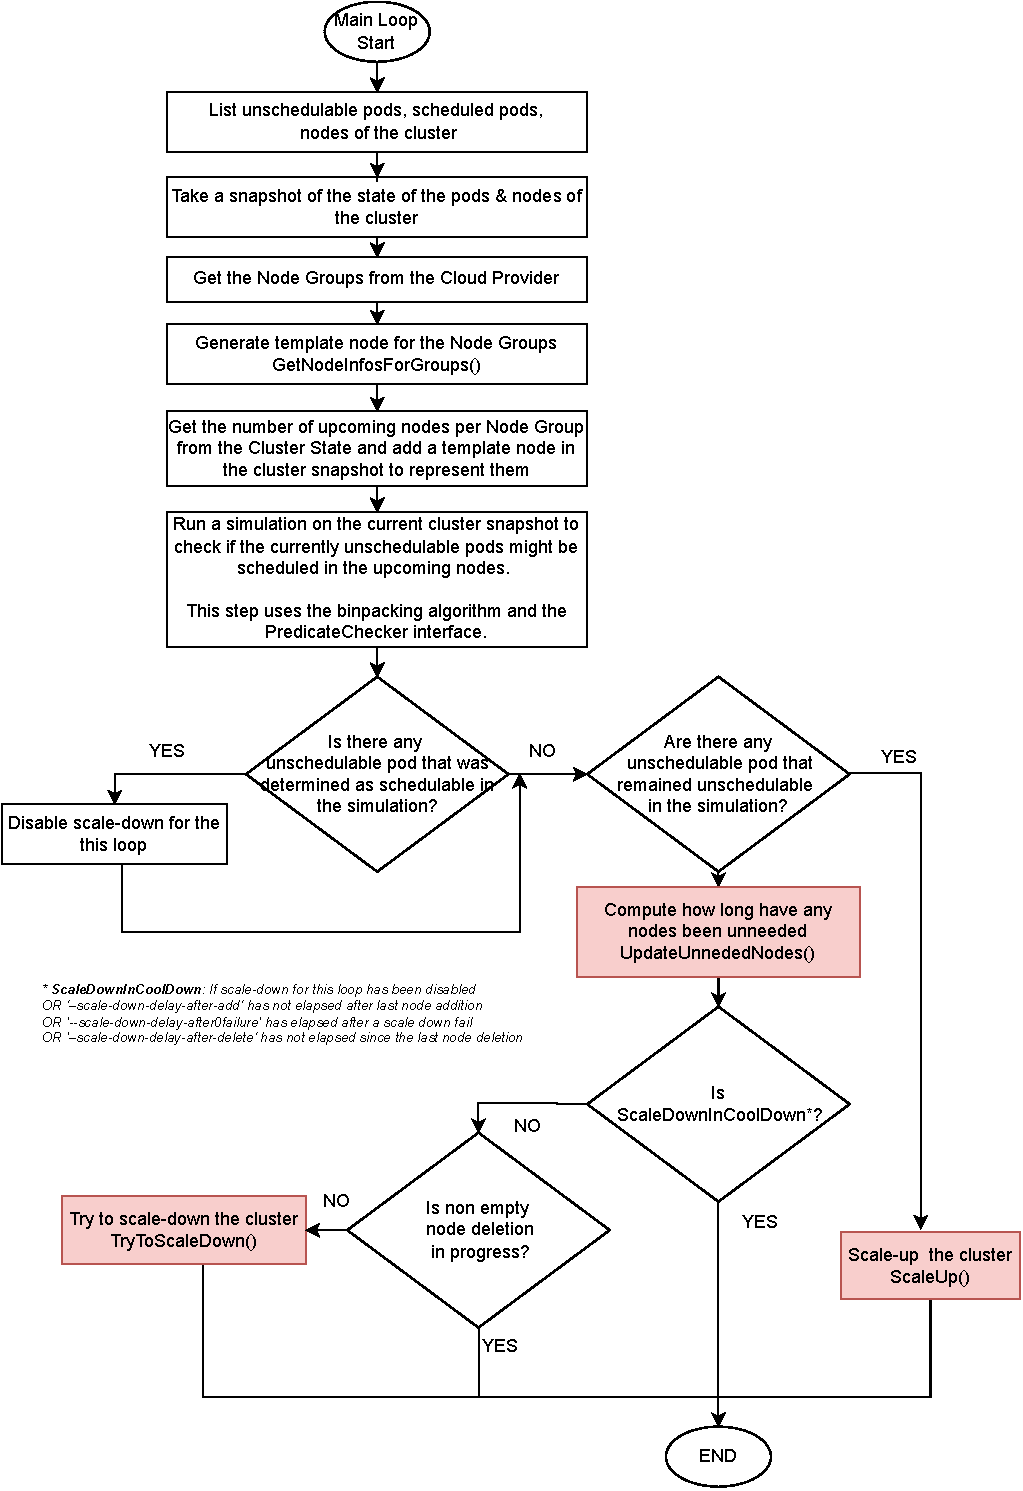
\includegraphics[width=\textwidth]{resources/autoscaler-main-loop.pdf}
      }
      \caption{Cluster Autoscaler:The main loop}
      \label{figure:autoscaler-main-loop}
\end{figure}


\subsection{Scale-Down}
\label{section:design-scale-down}
The Autoscaler tries to scale down the cluster if it did not attempt any
scale-up in the current run of the main loop. The scale-down procedure consists
of two distinct procedures:
\begin{enumerate}
      \tightlist
      \item \textit{Update unneeded nodes}: calculates which nodes have been
            unneeded and for how long.
      \item \textit{Try to scale down}: attempts to scale down the cluster by
            removing unneeded nodes.
\end{enumerate}

\begin{figure}[H]
      \centering
      \makebox[\textwidth][c]{
            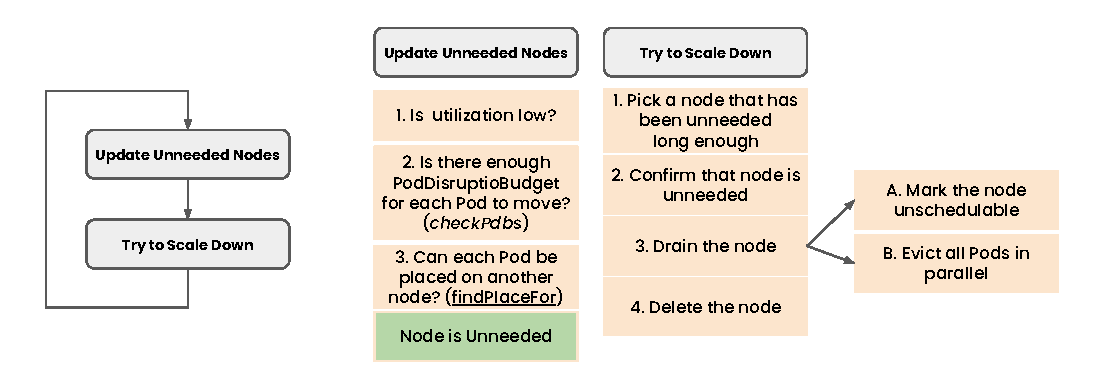
\includegraphics[width=1.1\textwidth]{resources/autoscaler-scale-down-process.pdf}
      }
      \caption{Cluster Autoscaler: Scale-down procedure}
      \label{figure:autoscaler-scale-down}
\end{figure}

We will use symbolic names to refer to various parameters of the Autoscaler in
our analysis, presented in Table \ref{table:symbolic-names-autoscaler}.
\begin{table}
      \begin{tabularx}{\linewidth}{|L|L|}
            \hline
            \textbf{Symbolic Name}        & \textbf{Description}                 \\ \hline
            scanInterval                  & How often cluster is reevaluated for
            scale up or down.
            \\
            \hline
            scaleDownDelayAfterAdd        & How long after scale up that scale
            down evaluation resumes. Defaults to 10 minutes. Configurable via
            the \co{--scale-down-delay-after-add} flag.                          \\
            \hline

            scaleDownDelayAfterDelete     & How long after node deletion that
            scale down evaluation resumes. Defaults to scanInterval.
            Configureable via the \co{--scale-down-delay-after-delete} flag.      \\
            \hline

            scaleDownDelayAfterFailure    & How long after scale down failure
            that scale down evaluation resumes. Defaults to 10 minutes.
            Configurable via the \co{--scale-down-delay-after-failure} flag.     \\
            \hline

            scaleDownUtilizationThreshold & Utilization threshold below which a
            node can be considered for scale down. Defaults to 0.5. Configurable
            via the \co{--scale-down-utilization-threshold} flag.                \\
            \hline

            scaleDownUnneededTime         & How long a ready node should be
            unneeded before it is eligible for scale down.  Defaults to 10
            minutes. Configurable via the \co{--scale-down-unneeded-time} flag.
            \\
            \hline

            scaleDownUnreadyTime          & How long an unready node should be
            unneeded before it is eligible for scale down.  Defaults to 20
            minutes. Configurable via the \co{--scale-down-unready-time} flag.
            \\
            \hline
      \end{tabularx}
      \caption{Symbolic names for various parameters of the Autoscaler used in our analysis}
      \label{table:symbolic-names-autoscaler}
\end{table}


\subsubsection{Update Unneeded Nodes Procedure}
The \textit{update unneeded nodes} procedure calculates which nodes of the
cluster have been unneeded and updates the Autoscaler's internal state with the
duration they have been unneeded. The Autoscaler considers a node
\textit{unneeded} if it meets all the following criteria:
\begin{itemize}
      \tightlist
      \item It is \textit{underutilized}, i.e., it has resource utilization
            below a specific threshold.
      \item The Pods that run on the node can be evicted (see section
            \ref{section:background-eviction}), i.e., their eviction is not
            blocked by any PodDisruptionBudgets.
      \item The Pods that run on the node can be moved to a different cluster
            node.
\end{itemize}
If a node does not meet the criteria, it is considered \textit{unremovable}.

To determine if an underutilized node is unneeded, the Autoscaler runs these
steps:
\begin{enumerate}
      \tightlist
      \item Calculate the Pods that must be moved if it removes the node.
      \item Check if any PodDisruptionBudgets block the eviction of any Pod. If
            so, the node is unremovable.
      \item Call \co{FindPlaceFor()} to find place for the Pods on a different
            node. \co{FindPlaceFor()} uses the
            \co{SchedulerBasedPredicateChecker} interface to determine if the
            Pod can be placed on any other node. It checks if the Pod can fit a
            node due to other scheduling constraints (CPU, memory), as well as
            if the Pod's volumes can be accessed from the node.
\end{enumerate}


The steps for  calculating the unneeded nodes are shown in
Algorithm~\ref{algo:update-unneeded}.

\subsubsection{Try to Scale Sown Procedure}

If a \textit{Ready} node remains unneeded for longer than
\co{scaleDownUnneededTime}, or an \textit{Unready} node remains unneeded for
longer than \co{scaleDownUnreadyTime} (see Table
\ref{table:symbolic-names-autoscaler} for the symbolic names) the Autoscaler
will consider the node as a candidate for deletion.

The Autoscaler makes a distinction between non-empty and empty nodes:
\begin{itemize}
      \tightlist
      \item \textit{Empty nodes}: nodes that run \textit{only} DaemonSet Pods.
            The Autoscaler removes them in bulk
      \item \textit{Non-empty nodes}: nodes that do not run only DaemonSet Pods.
            The Autoscaler removed them one by one to ensure that no Pods would
            be made unschedulable.
\end{itemize}

The algorithm for \co{TryToScaleDown()} is shown in
Algorithm~\ref{algorithm:try-scale-down}.

\paragraph*{Node removal} The node removal is executed as follows:
\begin{enumerate}
      \tightlist
      \item Add the \co{ToBeDeletedByClusterAutoscaler:NoSchedule} taint on the
            Node, essentially marking the node as unschedulable.
      \item Start draining the node by evicting in parallel all the Pods of the
            node. If any Pod can not be evicted due to a configured PDB, retry
            until the \co{MaxPodEvictionTimeout} exceeds.
      \item When all Pods are successfully evicted, ask the cloud provider to
            delete the node instance.
\end{enumerate}

The algorithm for the node removal is shown in
Algorithm~\ref{algorithm:node-delete}.


\clearpage
\begin{algorithm}[H]
    \caption{Cluster Autoscaler: Scale-down evaluation procedure}\label{alg:scale-down-evaluation}
    \SetKwIF{If}{ElseIf}{Else}{if~\endgraf}{\endgraf then}{else if}{else}{end if}%
    %\begin{minipage}{\textwidth}
    \begin{enumerate}[leftmargin=0cm]
        \tightlist
        \item Take a snapshot of the cluster Nodes, Pods, and PodDisruptionBudgets.
        \item \texttt{allNodes} \(\leftarrow\) List all the \co{Node} objects from the API Server.
        \item \texttt{scaleDownCandidates} \(\leftarrow\) Select nodes from
              \texttt{AllNodes} that belong to node groups that have not reached their
              minimum size.
        \item \texttt{podDestinations} \(\leftarrow\) \texttt{AllNodes};
              \texttt{podDestinations} represents the nodes that that may accept Pods in case a node is removed.
        \item Call \texttt{UpdateUnneededNodes()} with \texttt{podDestinations},
              and \texttt{scaleDownCandidates} as input, to calculate which nodes are
              unneeded an which ones are unremovable.
        \item \uIf{\begin{tabular}{@{\hspace*{1.0em}}l@{}}
                      the scale-down has been disabled for this loop                                           \\
                      % TODO: times in table
                      \textbf{OR} \co{scaleDownDelayAfterDelete} interval has not elapsed  \\
                      \textbf{OR} \co{scaleDownDelayAfterAdd} interval has not elapsed  \\
                      \textbf{OR} \co{scaleDownDelayAfterFailure} interval has not elapsed 
                  \end{tabular}}{
                  Don't scale-down the cluster. Autoscaler Status: \texttt{ScaleDownInCooldown}
              }
              \uElseIf{there is non empty node deletion in progress} {
                  Don't scale-down the cluster. Autoscaler Status: \texttt{ScaleDownInProgress}}
              \lElse{Try to scale down the cluster.}
    \end{enumerate}
    %\end{minipage}
\end{algorithm}


\begin{algorithm}[ht]
    \caption{Cluster Autoscaler: UpdateUnneededNodes() method}\label{algo:update-unneeded}
    \KwIn{\texttt{scaleDownCandidates}: a list of nodes that belong to
        node groups that have not reached their minimum size }
    \KwResult{Update the
        state of the Autoscaler with information about which nodes are unneeded}
    \begin{enumerate}[leftmargin=0.5cm]
        \tightlist
        \item For each node in \texttt{scaleDownCandidates}, call \texttt{checkNodeUtilization()}:
              \begin{enumerate}[]
                  \tightlist
                  \item \lIf{node has the ``ToBeDeletedByClusterAutoscaler'' taint}{ it is currently deleted, continue to next node}
                  \item \lIf{node has ``cluster-autoscaler.kubernetes.io/scale-down-disabled: true'' annotation}{continue to next node}
                  \item Calculate the utilization of the node.
                  \item \lIf{utilization is above threshold}{continue to next node}
                  \item Add the node \texttt{currentlyUnneededNodes}.
              \end{enumerate}
        \item \texttt{currentlyUnneededNonEmptyNodes} \lar From \texttt{currentlyUnneededNodes} select nodes that are not empty, i.e., they do not run only DaemonSet Pods.
        \item Call \texttt{findNodesToRemove(currentlyUnneededNonEmptyNodes)} to determine nodes that can be removed. For each node:
              \begin{enumerate}[]
                  \tightlist%        
                  \item Get the Pods that are running on the node and for each Pod:
                        \begin{enumerate}[leftmargin=0.5cm]
                            \tightlist
                            \item \lIf{the Pod has a Pod disruption budget that prevents its eviction}{the node is unremovable}
                            \item Call \texttt{findPlaceFor(pod)} to determine if it can be moved elsewhere.
                            \item \leIf{the Pod can not be moved elsewhere}{the
                                      node is unremovable}{the node can be removed, add it to
                                      \texttt{nodesToRemove}}
                        \end{enumerate}
              \end{enumerate}
        \item For each node in \texttt{nodesToRemove} update the state of the Autoscaler with the duration the node has been unneeded.
    \end{enumerate}
\end{algorithm}

\begin{algorithm}[ht]
\caption{Cluster Autoscaler: TryToScaleDown() method}\label{algorithm:try-scale-down}
    \KwIn{A list of unneeded nodes, as computed by UpdateUnneded() method}
    \KwResult{Scales-down the cluster}
\begin{enumerate}[leftmargin=0.5cm]
\item
  For each node in the unneeded nodes:

  \begin{enumerate}[leftmargin=0.5cm]
  \tightlist
  \item \lIf{If the node has the \texttt{cluster-autoscaler.kubernetes.io/scale-down-disabled}}{mark the node unremovable, reason \co{ScaleDownDisabledAnnotation}, go to next node.}
    \item
    \lIf{the node is \texttt{Ready}, and it has been underutilized for
    less than \texttt{ScaleDownUnneededTime}}{mark the node unremovable,
    reason \texttt{NotUnneededLongEnough}, continue to next node}
  \item
    \lIf{the node is \texttt{Unready}, and it has been underutilized for
    less than \texttt{ScaleDownUnreadyTime}}{mark the node unremovable,
    reason \texttt{NotUnreadyLongEnough}, continue to next node}
  \item
    Get the NodeGroup the node belongs to, get its \co{minSize} and current
    \co{size}, the number of node deletions in progress for the node group
    (\texttt{deletionsInProgress}).
  \item \lIf{\co{size} - \co{deletionsInProgress} $\leq$ \co{minSize}}{
    mark the node unremovable, reason \texttt{NodeGroupMinSizeReached},
    continue to next node}
  \end{enumerate}
  \item
  \co{candidates} \lar All the unneeded node that were not marked unremovable
  \item
    From \co{candidates}, try to scale-down as many as possible empty nodes.
  \item
    \texttt{nodesToRemove} \lar From the remaining candidates find nodes to
    remove (call \texttt{FindNodesToRemove()}).
  \item
    Pick a node from \texttt{nodesToRemove} and delete it
    (call \texttt{deleteNode()}) .
\end{enumerate}
\end{algorithm}
\begin{algorithm}[ht]
\caption{Cluster Autoscaler: deleteNode() method}\label{algorithm:node-delete}
    \KwIn{An unneeded Node of the Cluster to be deleted}
     \KwResult{Deletes the Node from the cluster and the Cloud Provider}
        \begin{enumerate}[leftmargin=0.5cm]
        \tightlist
        \item Add \co{ToBeDeletedByClusterAutoscaler:NoSchedule} taint on the
        Node to make the Node unschedulable.
        \item Drain the node; For each Pod (except for the DaemonSet Pods), in parallel:
            \begin{enumerate}
                \tightlist
                \item Send Eviction request
                \item \lWhile{the Eviction fails and for duration up to \co{MaxPodEvictionTimeout}}{retry the Eviction}

                Note: \co{MaxPodEvictionTimeout} is a hard-coded value equal to 2 minutes.
            \end{enumerate}
        \item \lIf{any of the Pods was not evicted successfully}{return error}
        \item \lIf{the node has any annotation with prefix
        \co{delay-deletion.cluster-autoscaler.kubernetes.io/}}{wait for up to
        \co{nodeDeletionDelayTimeout} for the annotation to be removed}
        \item Request from the Cloud Provider to delete the Node.
        \item \lIf{the Cloud Provider deletion fails}{return error}
        \end{enumerate}
\end{algorithm}


\clearpage
\subsection{Scale-Up}
\label{section:design-scale-up}
If the cluster has unschedulable Pods, the Autoscaler will try to help them by
adding new nodes to the cluster (\textit{scale-up}). A scale-up, essentially, is
the increase of the target size of one or more node groups. If multiple node
groups exist in the cluster, the cluster has to decide the following:
\begin{itemize}
      \tightlist
      \item Which node groups can help the unschedulable Pod run.
      \item How many nodes of the node group do the Pods need.
      \item If different node group scale-ups are feasible, which node group
            shall scale up.
\end{itemize}

As soon as the Autoscaler increases the target size of a node group, the cloud
provider will spin up new node instances, the new nodes will join the Kubernetes
cluster, and the scheduler will gradually scheduler the so far unschedulable
Pods to the new nodes.

The full algorithm for the \texttt{ScaleUp()} method is shown in
Algorithm~\ref{algorithm:scale-up}.

% TODO We show or is shown 
\paragraph*{Scale-up options}
To decide whether the scale-up of a node group would help the unschedulable Pod,
the Autoscaler runs the (roughly) following steps:
\begin{enumerate}
      \tightlist
      \item Take a snapshot of the cluster.
      \item Add a template node of the node group to the snapshot.
      \item Run a simulation, using the \co{SchedulerBasedPredicateChecker},
            whether the unschedulable Pod can be scheduled on the modified
            snapshot of the cluster.
      \item If the simulation determines that the Pod can be scheduled on the
            modified snapshot, use the \co{BinPackingNodeEstimator} to calculate
            how many nodes of that node group are needed.
\end{enumerate}

The option to scale up a specific node group with the number of needed nodes is
referred to as a ``\textit{scale-up option}''.

The complete algorithm to calculate a scale-up option is shown in Listing
\ref{algorithm:scaleup-options}.

\paragraph*{Scale-up strategy}

If multiple scale-up options, i.e., different node group scale-ups, can help the
unschedulable Pods, the Autoscaler decides which one is best using the
\co{Strategy} interface. There are various strategies, and the administrator can
configure the Autoscaler to use a desired one, e.g., the least cost option,
random strategy, etc.


\begin{algorithm}[ht]
    \caption{Cluster Autoscaler: ScaleUp() method}\label{alg:cap}
    \label{algorithm:scale-up} \KwIn{\co{pods}: the unschedulable Pods
        \\\co{snapshot}: the cluster snapshot } \KwResult{Adds extra nodes to
        accommodate the unschedulable Pods}
    \begin{enumerate}[leftmargin=0.5cm]
        \tightlist
        \item Build Pod equivalence groups - each Pod equivalence group consists
              of Pods that are managed by the same controller (same UUID) and have
              the same spec and labels.
        \item For each node group registered:
              \begin{enumerate}
                  \tightlist
                  \item Get its target size.
                  \item If the target size $\geq$ max size, go to the next node
                        group.
                  \item Create a template node for the node group.
                  \item Compute the expansion option for the node group, see
                        \co{ComputeExpansionsOption()}.
                  \item If any unschedulable Pod can be helped by adding a new
                        node of the node group, add the node group in the expansion
                        options list.
              \end{enumerate}
        \item If there are not any expansion options list, then do not trigger
              any scale-ups.
        \item Else, from the expansions options select one, according to the
              configured expansion strategy.
        \item Execute the selected scale up option: increase the target sizes of
              the corresponding node groups.
    \end{enumerate}
\end{algorithm}

\begin{algorithm}[ht]
    \caption{Cluster Autoscaler: ComputeExpansionsOption()
        algorithm}\label{algorithm:scaleup-options} \KwIn{\co{pods}: the unschedulable
        Pods \\\co{snapshot}: the cluster snapshot \\\co{template}: the template
        node of the node group} \KwResult{Computes if the scale-up of the node group
        would help any of the unschedulable Pods.}
    \begin{enumerate}[leftmargin=0.5cm]
        \tightlist
        \item
              For each Pod equivalence group:
              \begin{enumerate}
                  \tightlist
                  \item Get the sample Pod of the Pod equivalence group.
                  \item Add the template node in the cluster snapshot.
                  \item Call the Predicate Checker to check if any of the
                        unschedulable Pods can be scheduled in the new cluster snapshot.
                  \item If the sample Pod fits the new node in the cluster
                        simulation, append all the equivalent Pods in the list of Pods
                        that got helped (\co{options.Pods}).
              \end{enumerate}
        \item Call the bin-packing estimator to estimate how many nodes of
              the node group would be needed to help all the equivalent Pods.
        \item Return the \co{option}: a struct that indicates how many nodes of
              the node group are needed and which Pods would be helped.
    \end{enumerate}
\end{algorithm}



\clearpage
\subsection{Shortcomings \& Proposed Extensions}

In previous sections, we described the algorithms that govern the operations of
the Autoscaler; we will now identify their shortcomings.

\subsubsection{Scale-Down: Rok Volumes Can Be Migrated}
\label{section:design-autoscaler-unpinned}

When evaluating the scale-down of a node, the Autoscaler tries to find a place
for the Pods that run on the node in other cluster nodes. To do so, it calls the
\co{FindPlaceFor()} method, which in turn leverages the \co{PredicateChecker}
interface methods to determine if a Pod fits a node. The
\co{SchedulerBasedPredicateChecker} implementation of the interface runs the
VolumeBinding plugin's \co{Filter()} method to check if the volumes of the Pod
can be accessed from another node.


The PVs of the Rok storage class have node affinity that matches only with the
node where the volume was provisioned. Since the node affinity of the volumes
does not match any other in the cluster, the Autoscaler considers that the Pod
and its volume can not be moved on a different node, thus, marking the current
node as unremovable. The \co{SchedulerBasedPredicateChecker} does not know that
the Rok volumes have a mechanism to snapshot and recover them on a different
node [by unpinning them (snapshot + remove volume's node affinity, see section
            \ref{section:design-unpin}) and then pinning them (restoring the data) on
            another node ].

We propose the extension of the Autoscaler to simulate the Rok volumes as
unpinned (as if they do not have node affinity) when evaluating a scale-down
(and only then; in other cases, the volumes are retaining their node affinity).
With this extension, the Autoscaler will comprehend that the Rok volumes can
move anywhere in the cluster, and it can remove the node safely.

\subsubsection{Scale-Down: Coordinate With the Rok CSI Guard Mechanism}

As part of the Rok volume protection mechanism (see section
\ref{section:background-rok-csi-guard}), we deploy a \texttt{Deployment} object
for each node of the cluster, which creates a Pod per node (Rok CSI Guard)  with
strict node affinity that matches only the node it protects. The Autoscaler
tries \textit{to find place} to move this Pod. Since the Pod has strict node
affinity that matches only the current node, SchedulerBasedPredicateChecker
assumes that the Pod cannot be moved to a different node. Because of that, the
Autoscaler marks the node as unremovable. Of course, the Rok Operator will
remove the Pod after the Autoscaler removes the node, but the Autoscaler is
unaware of this fact.

Moreover,  the Autoscaler checks the PDB of the Guard Pod. The PDB of the Guard
Pod is configured to cause any evictions to fail. The Autoscaler notices that
and assumes that the Guard Pod will not be able to get safely evicted, thus,
marking the node unremovable. It is unaware that the Rok Operator will remove
them as soon as the scale-down starts and the Rok CSI  unpins all the local
volumes of the node.

We propose the extension of the Autoscaler so that it does not try to find a
place for the operator-managed ephemeral Guard Pods. Moreover, we extend the
Autoscaler to ignore the PDB of the Guard Pod. Still, the Autoscaler will be
aware that the Guard Pod exists, evicting it when it drains the node. This
eviction will fail as long as the PDB exists and the Autoscaler will retry,
delaying the deletion of the node.

To make things more obvious, here is the procedure that will take place with the
new design:


\begin{enumerate}
      \tightlist
      \item The Autoscaler evaluates a node for removal:
            \begin{enumerate}
                  \item It checks if the PDB allows the eviction of the Pods
                        running on the node, but it ignores the PDB of the Guard
                        Pod.
                  \item It tries to find a place for each Pod on a different
                        node, but it ignores the Guard Pod.
            \end{enumerate}
      \item The Autoscaler decides to remove the node.
      \item The Autoscaler adds the deletion taint on the node, effectively
            marking it as unschedulable for Pods.
      \item The Autoscaler sends eviction requests for each Pod to the API
            Server.
      \item The eviction of all the Pods --except for the Guard Pod-- succeeds.
      \item The Autoscaler keeps retrying to evict the Guard Pod, but the API
            Server responds that the eviction is not allowed due to the
            configured PDB.
      \item The Rok CSI Controller notices that the node is unschedulable and
            that no workload mounts the volumes, so it starts unpinning them.
      \item The Rok CSI Controller finishes the unpinning of the PVs.
      \item The Rok Operator removes the PodDisruptionBudget of the Guard Pod.
      \item The Autoscaler's request to evict the Guard Pod succeeds since the
            PDB was removed.
      \item The Autoscaler asks the cloud provider to delete the node.
      \item The Rok Operator removes the Rok CSI Guard \texttt{Deployment}
            object that corresponds to the removed node.
\end{enumerate}

Let us notice that the Autoscaler keeps retrying the eviction of the Guard Pod
for up to 2 minutes. That duration is a hard-coded timeout that might not be
enough in most cases. Taking a snapshot of the volume may last more than 2
minutes, depending on the size of the volume. It would be wise to use more sane
values and allow the user to cluster's admin to configure the value when
deploying the Autoscaler. To do so, we propose the extension of the Autoscaler
with a flag to configure the max pod eviction timeout.

\label{section:design-autoscaler-guards}


\subsubsection{Scale-Down: Consider Storage Capacity}

The Autoscaler shall check if the Rok volumes of a Pod can fit a node concerning
their requested storage capacity when evaluating a scale-down. As we have
explained, the Autoscaler used the \texttt{SchedulerBasedPredicateChecker}
interface in order to check if a Pod fits a node, which --among others-- calls
the VolumeBinding plugin's \co{Filter()} method.

We propose the extension of the SchedulerBasedPredicateChecker's VolumeBinding
plugin's \co{Filter} method: When evaluating if a Pod can be moved to a
different node, check if there is enough available storage on the node to move
the volumes.

Moreover, since the snapshotting and migration of a volume is a procedure that
costs in terms of time, the  Autoscaler shall not remove nodes with high storage
utilization, similarly to how it handles the CPU and memory resources. To
achieve this, we propose the extension of the Autoscaler with a new metric,
called the (Rok) ``\textit{storage utilization}'', defined as the ratio of the
used storage over the max storage capacity of the node. The Autoscaler will
compare this metric against a threshold configurable by the admin via a
corresponding flag; if the storage utilization exceeds the threshold, the node
will be considered unremovable.

\subsubsection{Scale-Down: Do Not Remove Unready Nodes}

A node that with status \co{Ready} can become \co{Unready} (or \co{NotReady}) if
a system problem on the node arises. Common reasons include lack of resources on
the node, a problem with the kubelet, an error related to kube-proxy, or a
networking problem in general.

The Autoscaler removes any unneeded Unready node after the
\texttt{scaleDownUnreadyTime} elapses. In the case of local volumes, we assume
that the node will always be in good condition, with all the systems up and
running and having network access, so Rok snapshots the local volumes to
Amazon's S3 remote storage. If that does not hold, removing a node will probably
cause any local data to be permanently lost.

The Autoscaler must not remove Unready nodes. The Unready nodes shall remain in
the cluster so that an administrator takes action to recover them from the
Unready state. We propose the extension of the Autoscaler with a flag to
explicitly disable the scale-down for nodes in \co{Unready} state and consider
them unremovable.

\subsubsection{Scale-Up: Consider Storage Capacity}
The Autoscaler does not know how much local storage is available when a new node
is spanned up and added to the cluster. The template node it creates from a live
node contains information only for the \textit{currently} free storage (of the
live node), reported on the capacity annotation by the storage driver (see the
proposed scheduler design, section \ref{section:capacity-annotation}). We need a
mechanism to know how much free storage a new node of a node group will have,
and the Autoscaler shall consider it in its simulations.

\paragraph*{Report max capacity}
Assuming that all the nodes in a node group have the same disk configuration and
max storage capacity, we can use the storage driver to report what the new
node's storage capacity would be on the \co{Node} objects. We propose the
extension of the Rok CSI Node component to report the max capacity of a node as
a label on the \co{Node} object. This label will be referred to as the
``\textit{max capacity label}'' \footnote{The \textit{Rok max capacity label}:
      rok.arrikto.com/max-instance-capacity}.

We use a label instead of an annotation because various cloud providers give the
cluster admins the option to pass labels to the node group node templates the
cloud provider plugin constructs. In case no live node for the node group
exists, the Autoscaler will construct the template from the cloud provider
plugin and have the configured admin labels on it.

At this point, let us distinguish the two reported quantities:
\begin{itemize}
      \tightlist
      \item \textit{capacity annotation}: the remaining free storage of a live
            node. The storage driver reports it, and the scheduler considers it
            when scheduling Pods.
      \item \textit{max capacity label}: the max storage capacity of the live
            node. i.e., the total storage capacity. That is a time constant
            value that depends on the node's disks.
\end{itemize}

For example, a node might have 200 Gi total storage (reported on the max
capacity label), and only 100 Gi out of them are free (reported on the capacity
annotation).

\paragraph*{Pass the max capacity information to the template}

For the Autoscaler to simulate the scheduling with capacity considerations, we
will import in the SchedulerBasedPredicateChecker the extended VolumeBinding
(see section \ref*{section:volume-plugin-extensions}).

The extended VolumeBinding plugin will look for the capacity of a template node
on the capacity annotation and not on the label. Since the template will get the
annotation from a live node, it will represent the currently free storage on the
live node instead of the max storage capacity. We need to sanitize the value and
set it to the actual max capacity. To do so, we propose the extension of the
sanitization mechanism of the Autoscaler to copy the max capacity label's value
to the capacity annotation. In this way, the template node's capacity annotation
will indicate the max capacity (total) storage of the new node of the node
group.

The sanitization mechanism shall set the capacity annotation to an infinitely
large value if the max capacity label does not exist. This design choice offers
the following advantages:
\begin{enumerate}
      \item The Autoscaler treats the node as if it had infinite storage
            capacity and will add a live node of the node group (scale-up). If
            the decision was wrong (\textit{false scale-up}), i.e., the added
            node does not have enough storage capacity for the Pod that
            triggered the scale-up, the scheduler of the cluster will not assign
            the Pod to the newly added node. As a result, the node will remain
            unneeded, and the Autoscaler will remove it after some time. The
            system will gradually fix the wrong decision.
      \item The wrong node addition allows the Autoscaler to learn the actual
            max capacity of the node. The Rok CSI driver gets the chance to run
            on the node, and the Autoscaler generates a template node from the
            live node, which contains accurate information for the max available
            capacity reported by the Rok CSI driver.
\end{enumerate}


\paragraph*{Wait for Rok CSI to run}

If a Pod triggers a scale-up because of the storage it requests, it may take a
reasonable time from the node addition till the Rok CSI driver starts running on
the node. As long as the Rok CSI is not running on the node, the corresponding
capacity annotation is not set on the \co{Node} object. The scheduler does not
schedule the Pod on the node since the absence of the annotation indicates the
storage is unavailable (see Section ~\ref{section:design-volume-binding}). The
Autoscaler runsthe scheduling simulation and decides that the Pod does not fit
the newly added node (since the live node has no capacity annotation), so it
triggers a new scale-up.

To resolve this issue, the Autoscaler must wait for the Rok CSI driver to run on
the newly added node. As long as the driver does not run on a new node (i.e.,
the node does not have the capacity label set), the Autoscaler shall replace the
node with an \textit{Unready} copy.

The Autoscaler treats Unready nodes as upcoming nodes (for a duration of up to
15 minutes): it replaces them with template nodes of the node group they belong
to in its simulations. The template node will have the capacity annotation set
as if the Rok CSI was running. The Autoscaler's simulation will assume that Pod
will be scheduled on the node when the Rok CSI is ready and running and will not
trigger any further scale-up.

We mentioned that the Autoscaler treats Unready node as upcoming for up to 15
minutes. That needs a bit of explanation. The Autoscaler gives the nodes a
reasonable amount to become fully Ready; after this duration, it will stop
replacing the Unready nodes with their template and will consider them
unschedulable in the simulation. If any Pods that relied on the node becoming
ready (in order to run there) still exist, they will now trigger another
scale-up. Of course, in the case of Rok, 15 minutes are more than enough for the
Rok CSI driver to become ready and start running.


\chapter{Implementation} \label{chapter:implementation}
In this chapter, we describe the implementation of the proposed design changes and the technologies used.

\section{Software Stack}

The proposed design involves many parts that we had to extend:
\begin{itemize}
      \tightlist
      \item Kubernetes Scheduler, written in Go.
      \item Kubernetes Cluster Autoscaler, written in Go.
      \item Rok CSI driver, written in Python.
\end{itemize}

It also introduces a new component, the Rok Scheduler webhook, which we wrote in
Go.

We build the components in a reproducible manner, using Docker containers for
the target language of each component. To describe and automate the build
process, we used Dockerfiles and Makefiles.

In order to deploy the components (Cluster Autoscaler, Rok Scheduler, Rok
Scheduler webhook) on the cluster, we write YAML manifests that use the
declarative API of Kubernetes to describe the necessary resources. To ease out
the manifests management, we use the \textit{Kustomize} tool. Kustomize is a
configuration management solution that leverages layering to preserve the base
settings of the applications and components by overlaying declarative YAML
artifacts (called patches) that selectively override default settings without
changing the original files.


\section{Extending the Rok CSI driver}

In order to extend the Rok CSI driver's node component with the capacity
reporting functionality, we introduce a new thread that periodically calculates
the capacity and updates the capacity on the \co{Node} object on the API Server. The
Python thread issues commands to the underlying Logical Volume Manager to fetch
the Rok VG size. We introduce an argument {\co{--capacity-poll-interval}} to
configure how long the thread waits before updating the storage capacity.


\lstinputlisting[label={listing:rok-capacity},language=Python,caption={The thread of Rok CSI driver that updates the available capacity}]{code/rok-capacity.python}

\section{Extending the Kubernetes Scheduler}

The VolumeBinding plugin of the Kubernetes Scheduler imports and uses the
\texttt{scheduling} package located at
\texttt{pkg/controller/volume/scheduling/scheduler\_binder.go}, in the
Kubernetes repo \footnote{\url{https://github.com/kubernetes/kubernetes}}. We
extend the package as follows:

\begin{itemize}
      \tightlist
      \item Introduce a \texttt{hasRokEnoughCapacity(claims\
            {[}{]}*v1.PersistentVolumeClaim,\ node\ *v1.Node)} method, which
            checks if there is enough capacity on the given \texttt{node} to
            provision all the specified Rok PVCs (\texttt{claims}). This method
            executes the following steps:
            \begin{enumerate}
                  \tightlist
                  \item Iterate through the given \co{claims}, and sum their
                        storage requests in
                        \texttt{totalRequestedCapacity}
                  \item Check if the given node has
                        \texttt{rok.arrikto.com/capacity} annotation.
                  \item If the annotation does not exist, or if it exists but is
                        not a valid int, returns \co{false}, which indicates the
                        PVCs can not be provisioned on the examined node.
                  \item If the annotation exists, fetch its value as
                        \texttt{nodeCapacityInBytes}.
                  \item If \texttt{totalRequestedCapacity} $\leq$
                        \texttt{nodeCapacityInBytes} return true, otherwise
                        false.
            \end{enumerate}
            The implementation of the method is exposed in listing
            \ref{listing:hasrokenough}.
      \item Extend the \texttt{checkVolumeProvisions()} method of the
            \co{VolumeBinding} plugin to gather all the Rok PVCs, (PVCs
            provisioned by \texttt{rok.arrikto.com}), and pass them to
            \texttt{hasRokEnoughCapacity()}, in order to check if there is
            enough capacity for all of them to be provisioned on a selected
            node. The implementation is show at Listing
            \ref{listing:checkvolumeprovisions}.
      \item Treat the case that the \texttt{rok.arrikto.com/capacity} does not
            exist as \texttt{zero} capacity, i.e., the volumes can not be
            provisioned.
\end{itemize}

\lstinputlisting[label={listing:hasrokenough},language=Golang,caption={Implementation of the hasRokEnoughCapacity() method}]{code/scheduler-rok-has-enough.go}
\lstinputlisting[label={listing:checkvolumeprovisions},language=Golang,caption={Extension of the checkVolumeProvisions() method}]{code/scheduler-volume-binding.go}

We compile the Rok Scheduler and build its Docker image using the Makefile the
upstream project provides. We use YAML manifests and the Kustomize tool to
deploy the Rok Scheduler as a \co{Deployment} along with any other RBAC
resources it needs for its operation.

\section{Implementing the Rok Scheduler Webhook}

We implement the Rok Scheduler webhook that will mutate the Pods to use the Rok
Scheduler, in a manner it can be reused and easily configured. 

We expose the following configuration options:
\begin{itemize}
      \item {\co{--annotation-optout}}:  Annotation key that if present
            on the Pod, the Pod will not be mutated. The default value is
            \co{arrikto.com/skip-rok-scheduler-webhook}. This parameters allows
            the user to skip the mutation of a Pod in the webhook server, even
            though the API server admitted that Pod for mutation. We will refer
            to it as the ``\textit{opt-out annotation}''.
      \item {\co{--namespaces-optin}}: A comma-separated list of
            namespaces or namespaces globs. If a Pod matches against one of
            these namespaces it will get mutated. The default value is
            \co{``*''}, which matches against all namespaces. We will refer to
            it as the ``\textit{opt-in namespaces}''.
      \item {\co{--scheduler-name}}: The name of the scheduler that will
            be set on the Pod. The default  value is \co{rok-scheduler}.
\end{itemize}
For a complete list of arguments, see the \co{main()} method of the webhook in
Listing \ref{listing:webhook-main}.

The \co{Handle()} method of the webhook handles a single admission request as
follows:
\begin{enumerate}
      \tightlist
      \item If the Pod it has the opt-out annotation, do not mutate it.
      \item Check the namespace of the Pod against each namespace glob. If
            the namespace does not match any glob, do not mutate it.
      \item In all other cases, mutate the Pod by adding the scheduler name on
            its \\ \co{spec.SchedulerName} field.
\end{enumerate}

For the full implementation of the method, see Listing
\ref{listing:webhook-handle}.

We implement the Rok Scheduler Webhook using the \co{webhook} package of the
controller-runtime library of Go. The Kubernetes controller-runtime is a set of
go libraries for building controllers. For implementing the glob functionality
of the \co{--namespaces-optin} flag, we used the \co{glob} module of Go. 

Finally, in order for the Pods to be admitted and sent to the webhook, we
instruct the API Server to do so by creating a \co{MutatingWebhookConfiguration}
object (see Listing \ref{listing:webhook-object}). The
MutatingWebhookConfiguration we specify admits any newly created Pods in
namespaces that match the specific namespace selector. The namespace selector
matches against any namespaces that have the label \co{control‐plane: kubeflow}.
We chose to admit Pods only in this namespace since the workload we want to
admit is created in that namespace, but of course, the Pods in any other
namespace can be admitted. The MutatingWebhookConfiguration specifies that the
API server contacts the webhook server at the \co{/mutate} endpoint. It also
specifies a \co{Fail} failure policy so that if the webhook crashes or stops
responding, the creation of new Pods will fail. That is important to ensure
every single Pod is admitted and mutated with the scheduler name.

\lstinputlisting[label={listing:webhook-main},language=Golang,caption={The main() method of the Rok Scheduler Webhook}]{code/mutating-webhook-main.go}
\lstinputlisting[label={listing:webhook-handle},language=Golang,caption={The Handle() method the Rok Scheduler Webhook}]{code/webhook.go}
\lstinputlisting[label={listing:webhook-object},language=yaml,caption={The Rok Scheduler's MutatingWebhookConfiguration}]{code/mutating-webhook.yaml}

To build the Rok Scheduler Webhook and its Docker image, we create a Dockerfile
that instructs the docker to build the binary inside a container that has the
required \texttt{Golang} dependencies. 

We deploy the Rok Scheduler and the Rok Scheduler as \co{Deployment} resources
(see \ref{section:deployment}). The manifests also specify other necessary
resources, such as Roles, RoleBindings, ServiceAccounts, ConfigMaps.

\section{Extending the Cluster Autoscaler}

\subsection{Scale-Down: Rok Volumes Can Be Migrated}
\label{section:implementation-migration}
As explained in the design proposal (see
\ref{section:design-autoscaler-unpinned}), we extend the Cluster Autoscaler to
treat the local volumes of the Rok Storage class as unpinned, i.e., as if they
have no affinities, when evaluating a possible scale-down. In all other cases,
the local volumes shall be evaluated as is, pinned, i.e., having their existing
node affinities. 

To implement the design, we extend the CheckPredicates interface's method with
an extra boolean argument, called \co{simulateUnpinnedVolumes}. We pass down
information from the PredicateChecker methods to the VolumeBinding plugin's
\co{checkBoundClaims()} method. The SchedulerBasedPredicateChecker creates a
\co{cycleState} (see section \ref{section:cycle-state} struct that the plugins
it runs can use for storing data. We extend the \co{cycleState}  with the same
boolean \co{simulateUnpinnedVolumes} field to pass down to the VolumeBinding
plugin information. The full flow of the information whether to simulate
unpinned volumes or not is illustrated in Figure ~\ref{fig:flow-simulate}.

\begin{figure}[ht]
      \centering
      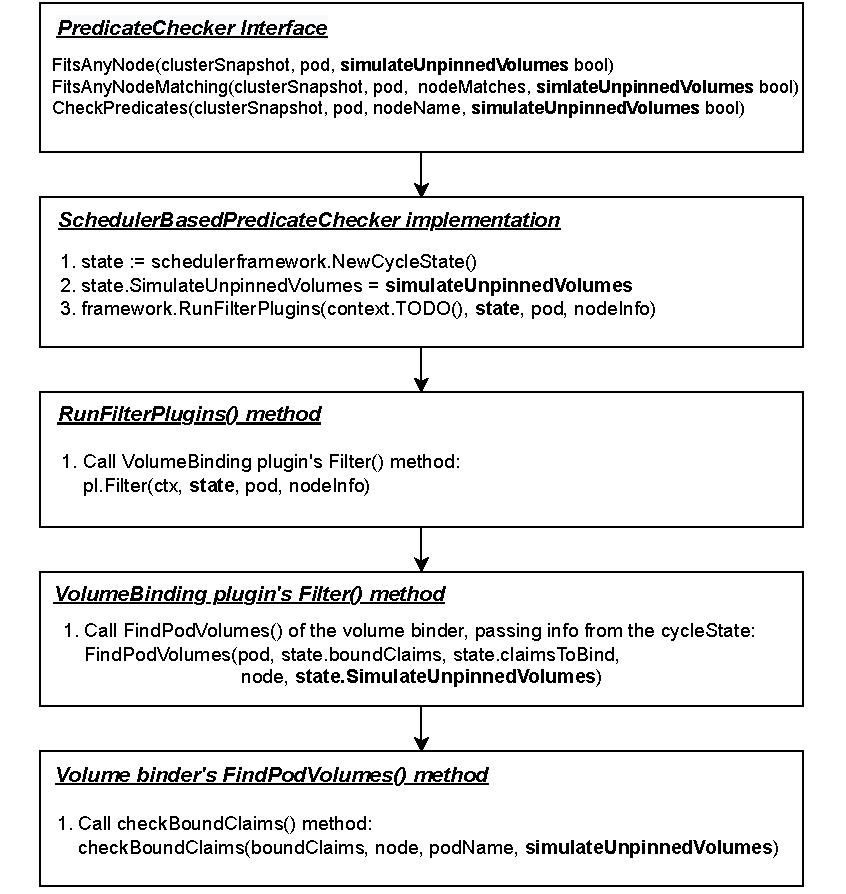
\includegraphics[width=0.8\textwidth]{resources/simulate-unpinned-flow.pdf}
      \caption{The flow of simulateUnpinnedVolumes information}
      \label{fig:flow-simulate}
\end{figure}


We extend the \co{checkBoundClaims()} method, so that if the Rok volumes are
simulated as unpinned (\co{simulateUnpinnedVolumes} is set to \co{true}), it
gathers all the Rok local volumes, and appends them to \co{claimsToProvision},
i.e, it treats them as if they were unbound volumes, in order to check if there
is enough capacity (see (\co{checkVolumeProvision()}) for the volumes to be
provisioned on the examined node. Of course, this approach only checks if the
Rok volumes of a Pod alone can be moved to a different node; it does not ensure
that all the Pods of the node can fit on a different node with regards to their
local storage requests. Listing \ref{listing:check-bound-claims} presents the
code lines that extend the functionality of \co{checkBoundClaims}.

\lstinputlisting[language=Golang,label={listing:check-bound-claims},caption={Extending the logic of checkBoundClaims() when volumes are simulated as unpinned}]{code/find-pod-volumes.go}


\subsection{Scale-Down: Coordinate With the Rok CSI Guard Mechanism}


To implement the design proposal (see section
\ref{section:design-autoscaler-guards}) we implement the following changes,
according to the proposed design:
\begin{itemize}
      \tightlist
      \item Extend the \co{findPlaceFor()} method to ignore the Rok CSI
            Guard Pods and not try to find a place for them on a different node.
      \item Extend the \co{checkPdbs()} method to not check the PodDisruptionBudgets
            of the Rok CSI Guard Pods.
      \item We introduce a flag \co{--max-pod-eviction-time}  so that the
      cluster admins can configure the maximum time Autoscaler tries to evict a Pod
      before giving up.
\end{itemize}

\lstinputlisting[language=Golang,label={listing:ignore-guard},caption={Ignore Rok CSI Guard Pods and their PDBs in scale-down evaluation}]{code/find-place-for.go}

%TODO: code snippet flag


\subsection{Scale-Down: Consider Storage Capacity}
We already covered in section \ref{section:implementation-migration} how we
extended the Autoscaler to simulate the Rok volumes as unpinned when scaling
down and also check if there is enough capacity for each Pod on a different
node.

We also extend the Autoscaler to calculate storage utilization and take it into
consideration when scaling down, by introducing a new flag
``--scale-down-rok-storage-utilization-threshold'' flag with default value
``0.5'' and a \co{CalculateUtilizationOfRokStorage()} method. This method
fetches the values from the capacity annotation and the max capacity label of
the \co{Node} object and calculates the storage utilization. Moreover, we extend
the \co{checkNodeUtilization()} method of the Autoscaler to mark any nodes that
have storage utilization over the storage threshold as unremovable. The
implementation can is shown in Listings \ref{listing:storage-util} and
\ref{listing:node-utilization}.

\lstinputlisting[label={listing:storage-util},language=Golang,caption={Calculate Rok storage utilization}]{code/rok-utilization.go}
\lstinputlisting[label={listing:node-utilization},language=Golang,caption={Mark nodes with high Rok storage utilization as unremovable}]{code/rok-utilization-threshold.go}


\subsection{Scale-Down: Do Not Remove Unready Nodes}

To implement the proposed design and configure the Autoscaler to not removed
unready nodes, we extend the \texttt{--scale-down-unready-time} of the
Autoscaler to accept negative values; if a negative value is provided, then the
scale-down of unready nodes will be disabled.

\subsection{Scale-Up: Consider Storage Capacity}

\paragraph*{Pass the max capacity information to the template}
To implement the scale-up design, we introduce a method
\co{sanitizeRokStorageAnnotations()} that copies the value of the max capacity
label of the \texttt{Node} object to its capacity annotation. If the label does
not exist, it set the capacity annotation to the max 64 bit number.We extend the
\co{sanitizeTemplateNode()} method to call \co{sanitizeRokStorageAnnotations} as
part of the sanitization process.

The implementation of this functionality is shown in Listings
\ref{listing:sanitize-rok} and \ref{listing:sanitize}.

\lstinputlisting[language=Golang,label={listing:sanitize-rok},caption={sanitizeRokStorageAnnotations() method}]{code/scale-up-capacity-label.go}
\lstinputlisting[language=Golang,label={listing:sanitize},caption={Extend sanitizeTemplateNode() to sanitize the Rok storage annotations}]{code/note-template-capacity.go}

\paragraph*{Wait for Rok CSI to run}

We implement this design change by introducing a
\co{FilterOutNodesWithUnreadyCSI()} method to check if a node has the capacity
annotation set. If not, it is implied that the Rok CSI driver is not running on
the node, and it replaces the node with an unready copy. We extend the
\co{obtainNodeLists()} method, to call the \co{FilterOutNodesWithUnreadyCSI}.

Listings \ref{listing:unready-csi} and \ref{listing:unready-csi-obtain} present
the code lines that implement this functionality.

\lstinputlisting[label={listing:unready-csi},language=Golang,caption={FilterOutNodesWithUnreadyCSI() method}]{code/unready-csi.go}
\lstinputlisting[label={listing:unready-csi-obtain},language=Golang,caption={Extend ObtainNodesLit() method to return nodes with unready Rok CSI}]{code/obtain-nodes-list.go}

\chapter{Conclusion} \label{chapter:conclusion}

Our journey has finally reached its end. In this chapter, we will restate our
contributions and summarize what our mechanism offers. Finally, we will close
this thesis by mentioning future work that can be done to enrich our mechanism
and bring it to its full potential.

\section{Concluding Remarks} \label{section:conclusion_concluding_remarks}

All in all, the primary goal of this thesis was to implement a design that would
enable seamless cluster autoscaling and scheduling with local persistent
storage. Not only did we achieve this goal, but our implementation was
successfully deployed to large production clusters of enterprises that requested
the feature.

Although the design we implemented is coupled with the Rok software --since it
provides an efficient mechanism for migrating local volumes around a cluster--,
the concepts and the design can be generalized to work with any other local
storage system. Our long-term goal, which extends beyond the context of this
thesis, is to generalize the design and push it upstream. That is a process that
we started to be involved in; we attend the meetings of the Kubernetes Storage
\footnote{https://github.com/kubernetes/community/blob/master/sig-storage/README.md}
and Autoscaling
\footnote{https://github.com/kubernetes/community/blob/master/sig-autoscaling/README.md}
Special Interest Groups, interacted with them on GitHub and plan to contribute
the whole design upstream actively. At the moment this text is written, we have
a few first Pull Requests merged
\footnote{https://github.com/kubernetes/autoscaler/pull/4877}
\footnote{https://github.com/kubernetes/autoscaler/pull/4842}.

\section{Future Work} \label{section:conclusion_future_work}

So far, we have implemented various enhancements for the Kubernetes Scheduler
and the Cluster Autoscaler, but there is always room for improvement. Since this
is an iterative process, in next iterations, we would like to offer these
enhancements:

\begin{itemize}
      \item Extend the Scheduler to reserve the storage (in the \co{Reserve}
            phase of the scheduling cycle) when scheduling a Pod to prevent race
            conditions.
      \item Extend the Cluster Autoscaler to consider the storage needed for the
            PVCs of multiple Pods when scaling down. The current design only
            checks if a single Pod's PVs can fit a node, but not if the PVs of
            multiple Pods fit a node. Although a wrong decision to scale down
            will be reverted by a subsequent scale-up, taking the decision would
            be much more effective.
      \item Extend the current implementation of the \co{Estimator} interface,
            i.e., the \co{BinPackingEstimator}, to consider the storage and
            calculate how many nodes are needed for the storage requests of
            multiple Pods of a StatefulSet. The current design adds nodes one by
            one till all the Pods get the requested storage. It would be much
            more efficient to know the number of nodes needed beforehand and add
            them to the cluster all at once.
\end{itemize}

Finally, as we already mentioned, our high-priority goal is to merge this work
upstream.

\setcounter{chapter}{0}

\selectlanguage{english}
\chapter{\introname} \label{chapter:introduction}

% See https://github.com/arrikto/prv-diplom/issues/8 for the rationale behind
% these chapters. We follow the structure proposed in
% https://cs.stanford.edu/people/widom/paper-writing.html.

In this first chapter, we outline the scope of our work. We provide a brief
overview of the task at hand, and we illustrate the gap that there is to fill.
Then, we review the existing approaches, highlighting their offerings and
drawbacks. Moving on, we give a high-level overview of the mechanism we built.
Finally, we present the structure of this thesis


\section{Motivation} \label{section:intro_motivation}


Kubernetes is the de-facto container orchestrator choice for every company going
cloud-native. The popularity of Kubernetes arises from the fact that it makes
application lifecycle management for container-based applications a lot easier
for DevOps via a declarative desired state-based management approach. It exposes
a powerful declarative API that developers can use to describe the desired state
of an application in terms of Pods, Services, etc. Kubernetes controllers take
immediate actions to bring the observed state of the system to the desired
state. Kubernetes can run on-premises and on most major cloud providers such as
Amazon Web Services (AWS), Google Cloud, and Microsoft Azure, which is also key
to its success.

By packaging code and dependency into containers, the development teams can use
standard code units that start and terminate quickly to allow applications to
scale to any size. They can use containers to package entire applications and
move them to the cloud without needing to undergo code changes. Kubernetes act
as an orchestrator platform to let large numbers of containers work harmoniously
together and reduce operational burdens.

The Kubernetes Scheduler and Cluster Autoscaler (Autoscaler) work together to
ensure the cluster's workload is running. The Scheduler ensures that the
workload units (Pods) are assigned to cluster nodes with sufficient resources,
i.e., memory, CPU, and storage. At the same time, the Cluster Autoscaler
maintains an appropriate number of nodes in the cluster that allows the workload
to run seamlessly without wasting any excess resources. The latter implies that
the Cluster Autoscaler is a component that enables enterprises to optimize costs
by dynamically scaling the number of nodes in the cluster in response to the
current cluster workload and, thus, meet dynamic demand. Without the Cluster
Autoscaler, the enterprises are bound to use a fixed-size cluster, which leads
to either being charged for unneeded resources in the cluster, or the necessary
resources would not be enough for the workload to run.

Combining Kubernetes with local persistent volumes allows users to access the
local storage of a node in the cluster through the standard Kubernetes
\texttt{PersistentVolumeClaim} interface in a simple and portable way. The
primary benefit of local persistent volumes over remote persistent storage
(e.g., network-attached volumes) is performance: local disks usually offer
higher IOPS, higher throughput, and lower latency than remote storage systems.
For instance, by attaching non-volatile memory express (NVMe) disks to a node,
the end-user can benefit from a huge performance boost when executing
applications that demand heavy storage utilization. For instance, in the case of
enterprises, local storage can enable them to optimize the speed that they run
the disk-intensive workload, such as machine learning, big data analysis tasks,
etc., which is a crucial factor for revenue.

Enabling the seamless operation of the Cluster Autoscaler on Kubernetes clusters
that leverage local storage is of high importance for enterprises. Local storage
will enable them to run disk-intensive workload efficiently and fast, the
Cluster Autoscaler will maintain the appropriate size of the cluster and the
Autoscaler will ensure that workload runs on the right kind of node. This triple
combination works towards infrastructure cost reduction, which is highly
important for enterprises.


However, working with local persistent storage has a few implications that
Kubernetes has not yet resolved:
\begin{itemize}
      \tightlist
      \item The Scheduler does not consider the available local storage when
            scheduling the workload units.
      \item The Cluster Autoscaler does not scale down (remove nodes) the
            cluster if local volumes are provisioned on the nodes since the removal
            would lead to data loss.
      \item The Cluster Autoscaler does not scale up the cluster (add nodes)
            when the nodes do not have enough local storage for the workload requests.
\end{itemize}

Motivated by the significance and the impact of using local persistent storage
on Kubernetes clusters, in this thesis, we propose extensions for the Kubernetes
Scheduler and the Cluster Autoscaler to enable seamless operation with local
storage. More specifically, our work is two-fold:

\begin{itemize}
      \item We propose a extensions so that the Cluster Autoscaler can scale
            down and up clusters with local persistent storage.
      \item We propose extensions for the Scheduler to schedule the workload on
            nodes with the required amount of local storage available.
\end{itemize}


\section{Problem Statement} \label{section:intro_problem_statement}

As stated in section \ref{section:intro_motivation}, this thesis is motivated by
local persistent storage's benefits. However, the integration of the Kubernetes
Scheduler and the Cluster Autoscaler with local storage has a few implications
that are not yet resolved:
\begin{itemize}
      \tightlist
      \item The Scheduler does not schedule the workload considering the
            available storage. Without considering the available storage, it may
            schedule a Pod onto an unsuitable node where the storage driver
            cannot provide the requested volumes because the underlying storage
            system does not have sufficient capacity.
      \item The Cluster Autoscaler does not scale down clusters with local
            persistent storage since the local data reside on each node, and
            removing the node would lead to losing access to these data.
      \item The Cluster Autoscaler does not scale up clusters, i.e., it does not
            add nodes in the cluster when there is not enough local storage for
            the workload to run.
\end{itemize}

In this thesis, we make design proposals and implement them to overcome these
problems and enable the seamless operation of the Kubernetes Scheduler and the
Cluster Autoscaler with local persistent storage.

%\section{Current Challenges} \label{section:intro-challenges}

\section{Existing Solutions} \label{section:intro-existing}

Currently, the Cluster Autoscaler does not support autoscaling for cluster nodes
that use local persistent storage. Each volume that is leveraging local storage
will be considered by the Autoscaler to be only accessible by that node, and,
thus, it will not remove the node where the data live; in other words, scaling
down with local volumes is infeasible. Moreover, there is no option to scale up
when there is not enough local storage for the workload that requests it. There
are no existing solutions to fix these problems.

Regarding the Kubernetes Scheduler, the Kubernetes community has currently
implemented preliminary support for scheduling with storage consideration. They
call the feature ``Storage Capacity Tracking''. Scheduling a Pod with Capacity
storage capacity tracking allows the storage (CSI) drivers to publish
information about the remaining capacity on each topology segment of the
cluster. The Scheduler then uses that information to pick a suitable node for a
Pod that requests volumes to be provisioned. However, the current approach comes
with a few limitations:

\begin{itemize}
      \item It does not attempt to model how scheduling decisions affect storage
            capacity. The Kubernetes SIG Storage team took this design decision
            to ease the development of the feature, since the effect can vary
            considerably depending on how the storage system handles storage. As
            a consequence of this decision, a Pod requesting multiple volumes to
            be provisioned might get scheduled on a node where there is only
            enough space for each of the volumes individually, without
            considering the total amount of storage needed to accommodate all
            the volumes. As a consequence, the scheduling of a Pod can fail
            permanently: one volume might get created successfully in a topology
            segment that does not have enough capacity left for the other
            volume. Then, the already provisioned volume will restrict future
            attempts to schedule the Pod. Manual intervention is necessary to
            recover from this state, for example, by increasing capacity or
            deleting the already created volume.
      \item The feature is only available on clusters running Kubernetes version
            1.21 or later. Running Kubernetes 1.21 or later is a requirement
            that not all production clusters currently meet. In our case, a few
            enterprises are still using older versions of Kubernetes; thus, the
            Capacity Tracking feature not available.
\end{itemize}

As it comes for the Cluster Autoscaler, there are no reported solutions to
overcome its current limitations.

\section{Proposed Solution} \label{section:intro_proposed_solution}

As already explained in previous sections, this thesis aims to enable seamless
autoscaling and scheduling on clusters that leverage local persistent storage.
Our proposed design involves the extension of various components, namely, the
Scheduler, the Cluster Autoscaler, and the controller of the local storage
driver (CSI driver).

In a nutshell, we propose the following design:

\begin{itemize}
      \item Extend the Rok CSI storage driver to report the available storage
            capacity on each cluster node on the Kubernetes \texttt{Node}
            objects. The driver will calculate the available storage by issuing
            commands to the underlying Local Volume Manager.
      \item Extend the Kubernetes Scheduler to consider the reported storage
            capacity of each node when scheduling a Pod that requests Rok's
            local volumes to be provisioned. We call the extended scheduler
            ``Rok Scheduler''.
      \item Integrate the Cluster Autoscaler with the Rok CSI mechanism to
            snapshot and protect local volumes when a node is removed, enabling
            the cluster's seamless scale-down.
      \item Extend the Kubernetes Cluster Autoscaler to consider the storage
            utilization when deciding whether to scale down a node and check if
            there is enough storage on other nodes to accommodate the Pods of
            the node.
      \item Extend the Kubernetes Cluster Autoscaler to scale up the cluster
            when there is insufficient storage.
      \item Extend the Kubernetes Cluster Autoscaler not to remove nodes of a
            cluster that are in the Unready state since the local volumes still
            live on the Unready nodes, and the removal of the node will lead to
            data loss.

\end{itemize}

In the context of this thesis, we use the ``Rok'' data management system by
Arrikto, which integrates with Kubernetes using the Container Storage Interface
(see section \ref{section:background-csi}) and exposes the local storage of a
node as volumes for the workload to consume.  Although the design implementation
focuses on Rok, it can be easily generalized to any other local storage systems.

\section{Outline}
\label{section:intro_outline}

The rest of this thesis is organized as follows:

\begin{itemize}
      \item In \textbf{chapter 2} we provide the theoretical background
            necessary for the reader to understand our work.
      \item In \textbf{chapter 3} we analyze the design of the Scheduler and the
            Cluster Autoscaler, expose parts of their mechanism and propose
            design changes for enabling their seamless operation when local
            persistent storage is involved.
      \item In \textbf{chapter 4} we analyze the implementation of our design.
      \item In \textbf{chapter 5} we provide a summary of our contributions and
            possible future work directions.
\end{itemize}
\chapter{Background} \label{chapter:background}

In this chapter, we provide the theoretical background necessary for
understanding the core practical ideas of the rest of the thesis.

\section{Architectural Evolution}

The popularity of microservices and containerization has exploded in recent
years. The need for scalable, easily deployable applications has led to 
abandoning monolithic architectures, where all processes are tightly coupled
and run as a single service, in favor of microservices. Microservices are an
architectural and organizational approach for software development where software
is composed of small independent services that communicate over well-defined
APIs.

The current industry trend for microservices is to use containerization to
deliver smaller, single-function modules, which work together to create more
agile, scalable applications. Containerization is a form of virtualization where
applications run in isolated user spaces, called containers, while using the
same shared operating system. A container is essentially a fully packaged and
portable computing environment. Everything an application needs to run --its
binaries, libraries, configuration files, and dependencies-- are encapsulated and
isolated in their container.

The extensive use of containers has driven the need to automate containers'
deployment and management. Container orchestration automates the operational
effort required to run containerized workloads and services. Container
orchestration includes various actions software teams need to manage a
container's lifecycle, including provisioning, deployment, scaling (up and
down), networking, load balancing, and more.

Kubernetes is the most popular solution among various container orchestrators
and has become the industry standard. Initially launched by Google, Kubernetes
is a portable, extensible, open-source platform for managing containerized
workloads and services that facilitates declarative configuration and
automation.

\begin{figure}
    \centering
    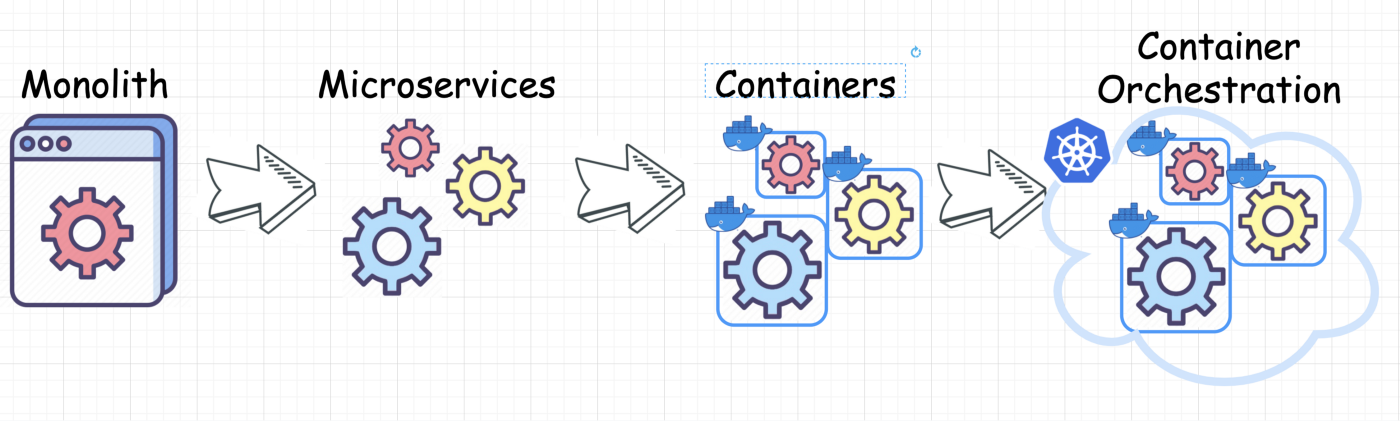
\includegraphics[width=0.8\textwidth]{resources/containerization.png}
    \caption{Architectural evolution: From monolithic applications to containerized microservices that are managed by a container orchestrator}
\end{figure}

Kubernetes operates on a cluster. A Kubernetes cluster is a set of node machines
for running containerized applications. The cluster is the heart of Kubernetes'
key advantage: the ability to schedule and run containers across a group of
machines, be they physical or virtual, on-premises or in the cloud.

\section{Kubernetes Fundamentals}


Kubernetes is an open-source orchestrator for deploying containerized
applications. It was initially developed by Google, inspired by a decade of
experience deploying scalable, reliable systems in containers via
application-oriented APIs. Since its introduction in 2014, Kubernetes has grown
to be one of the world's largest and most popular open-source projects. It has
become the standard API for building cloud-native applications in nearly every
public cloud. Kubernetes is a proven distributed system infrastructure suitable
for cloud-native developers of all scales. It provides the software necessary to
build and deploy reliable, scalable distributed systems.

\begin{figure}
	\centering
	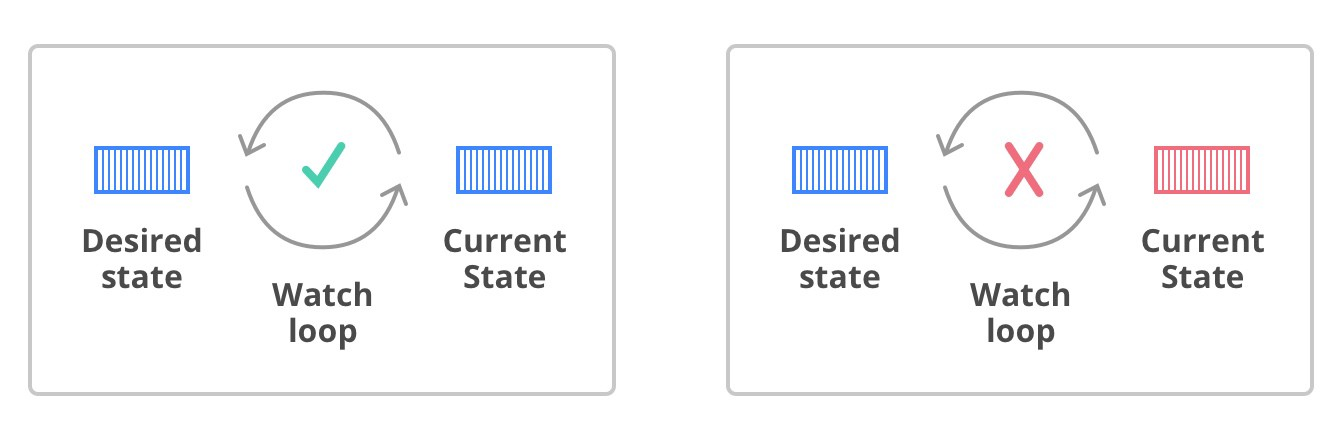
\includegraphics[width=0.8\textwidth]{resources/declarative.jpg}
	\caption{The Kubernetes reconciliation loop}
	% TODO: Replace scheme with the one from vkoukis
\end{figure}

Kubernetes makes application lifecycle management for container-based
applications much more effortless for DevOps via a declarative desired
state-based management approach. It exposes a powerful declarative API that
developers can use to describe the desired state of an application in terms of
Pods, Services, etc., and Kubernetes controllers will take immediate actions to
bring the observed state of the system to the desired state.

\subsection{Kubernetes Architecture}
A Kubernetes cluster consists of a set of worker machines, called nodes, that
run containerized applications. Every cluster has at least one worker node. The
worker nodes host the Pods, which are the components of the application
workload. The control plane manages the worker nodes and the Pods in the
cluster. In production environments, the control plane usually runs across
multiple computers, and a cluster usually runs multiple nodes, providing fault
tolerance and high availability.

\begin{figure}
	\centering
	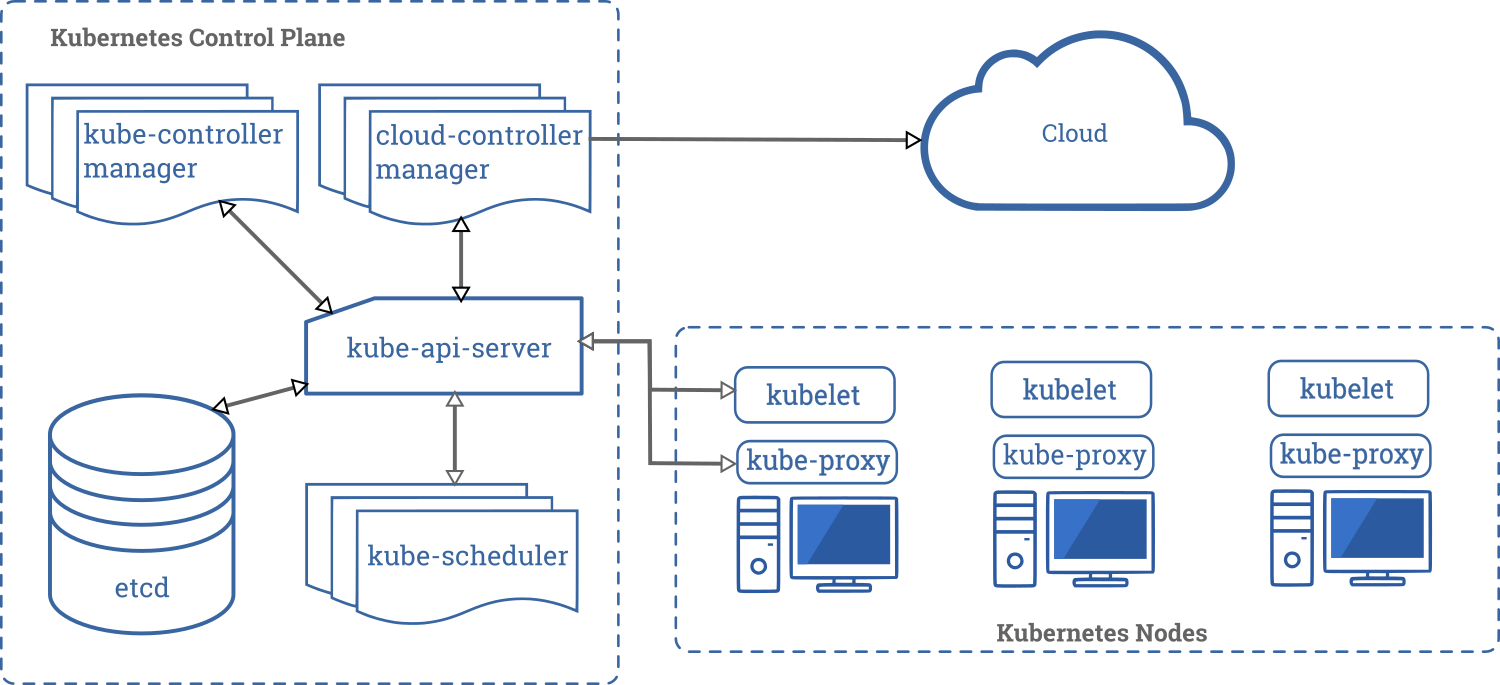
\includegraphics[width=\textwidth]{resources/components-of-kubernetes.png}
	\caption{Kubernetes Architecture}
\end{figure}


\subsection{Kubernetes Control Plane Components}
The control plane's components make global decisions about the cluster (for
example, scheduling), as well as detecting and responding to cluster events (for
example, starting up a new Pod when a deployment's replicas field is
unsatisfied).

The main control plain components are:

\begin{itemize}
	\item
	      \texttt{kube-apiserver}: The API server is a component of the
	      Kubernetes control plane that exposes the Kubernetes API. The API
	      server is the front end of the Kubernetes control plane. The primary
	      implementation of a Kubernetes API server is \co{kube-apiserver}.
	      \co{Kube-apiserver} is designed to scale horizontally, i.e., it scales
	      by deploying more instances. A cluster may run several instances of
	      \co{kube-apiserver} and balance traffic between those instances.
	\item
	      \texttt{etcd}: A consistent and highly-available key-value store that
	      is used as Kubernetes' backing store for all cluster data. Distributed
	      and fault-tolerant, etcd is an open-source, key-value store database
	      that stores configuration data and information about the state of the
	      cluster. Etcd may be configured externally, although it is often part
	      of the Kubernetes control plane.

	      Etcd stores the cluster state based on the Raft consensus algorithm.
	      This helps cope with a common problem in the context of replicated
	      state machines and involves multiple servers agreeing on values. Raft
	      defines three different roles: leader, candidate, and follower, and
	      achieves consensus by electing a leader.

	      In this way, etcd acts as the single source of truth (SSOT) for all
	      Kubernetes cluster components, responding to queries from the control
	      plane and retrieving various parameters of the state of the
	      containers, nodes, and Pods and other cluster components, in general.


	\item
	      \texttt{kube-scheduler}: Control plane component that watches for
	      newly created Pods with no assigned node and selects a node for them
	      to run on. Factors considered for scheduling decisions include
	      individual and collective resource requirements,
	      hardware/software/policy constraints, affinity, and anti-affinity
	      specifications, data locality, inter-workload interference, and
	      deadlines.
	\item
	      \texttt{kube-controller-manager}: Control plane component that runs
	      controller processes. Logically, each controller is a separate
	      process, but to reduce complexity, they are all compiled into a single
	      binary and run in a single process. Some types of these controllers
	      are:
	      \begin{itemize}
		      \tightlist
		      \item
		            \textbf{Node controller}: Responsible for noticing and
		            responding when nodes go down.
		      \item
		            \textbf{Job controller}: Watches for \co{Job} objects that
		            represent one-off tasks, then creates Pods to run those
		            tasks to completion.
		      \item
		            \textbf{Endpoints controller}: Populates the Endpoints
		            object (that is, joins Services \& Pods).
		      \item
		            \textbf{Service Account} \& \tbf{Token controllers}: Create
		            default accounts and API access tokens for new namespaces.
	      \end{itemize}
	\item
	      \texttt{cloud-controller-manager}: Kubernetes control plane component
	      that embeds cloud-specific control logic. The cloud controller manager
	      lets a user link their cluster into their cloud provider's API, and
	      separates out the components that interact with that cloud platform
	      from components that only interact with their cluster. The
	      cloud-controller-manager only runs controllers that are specific to
	      your cloud provider. If a Kubernetes cluster runs on a user's
	      premises, the cluster does not have a cloud controller manager.
\end{itemize}

\subsection{Kubernetes Node Components}

Node components run on every node, maintaining running Pods and providing the
Kubernetes runtime environment.

Every node runs the following components:

\begin{itemize}
	\item
	      \texttt{kubelet}: An agent that makes sure that containers are running
	      in a Pod.
	\item
	      \texttt{kube-proxy}: kube-proxy is a network proxy implementing part
	      of the Kubernetes Service concept. Kube-proxy maintains network rules
	      on nodes. These network rules allow network communication to the
	      user's Pods from network sessions inside or outside of their cluster.
	      Kube-proxy uses the operating system packet filtering layer if there
	      is one and it's available. Otherwise, kube-proxy forwards the traffic
	      itself.
	\item
	      \texttt{Container Runtime}: The container runtime is the software that
	      is responsible for running containers. Kubernetes supports container
	      runtimes such as containerd, CRI-O, and any other implementation of
	      the Kubernetes CRI (Container Runtime Interface).
\end{itemize}

\subsection{The Kubernetes API}

The core of Kubernetes' control plane is the API server. The API server exposes
an HTTP API that lets end-users, different cluster parts, and external
components communicate. The Kubernetes API lets the user query and manipulate
the state of API objects in Kubernetes (for example, Pods, Namespaces,
ConfigMaps, and Events). Kubernetes generally leverages common RESTful
terminology to describe the API concepts:


\begin{itemize}
	\tightlist
	\item A \textit{resource type} is the name used in the URL (Pods,
	      Namespaces, Services).
	\item All resource types have a concrete representation (their object
	      schema) which is called a \textit{kind}.
	\item A list of instances of a resource is known as a \textit{collection}.
	\item A single instance of a resource type is called a resource and usually
	      represents an object.
\end{itemize}

Almost all object resource types support the standard HTTP verbs - \texttt{GET},
\texttt{POST}, \texttt{PUT}, \texttt{PATCH}, and \texttt{DELETE}. Kubernetes
also uses its own, often written lowercase, to distinguish them from HTTP verbs.
Kubernetes uses the term ``list'' to describe returning a collection of
resources to distinguish from retrieving a single resource, usually called a
``get''. All resource types are scoped either to the cluster or to a
\textit{namespace}. A namespace-scoped resource type will be deleted when its
namespace is deleted, and access to that resource type is controlled by
authorization checks on the namespace scope.

\subsection{Kubernetes Objects}

Kubernetes \textit{objects} are persistent entities in the Kubernetes system.
Kubernetes uses these entities to represent the state of the cluster.
Specifically, they can describe:
\begin{itemize}
	\tightlist
	\item What containerized applications are running and on which nodes.
	\item The resources available to those applications.
	\item The policies around how those applications behave, such as restart
	      policies, upgrades, and fault-tolerance.
\end{itemize}

A Kubernetes object is a ``record of intent''; once a user creates the object,
the Kubernetes system will constantly work to ensure that the object exists. By
creating an object, a user is effectively telling the Kubernetes system what
they want their cluster's workload to look like.

%TODO: Add about put update delete patch
%https://kubernetes.io/docs/reference/using-api/api-concepts/

\subsubsection{The \co{Pod} Object}\label{background:Pod}

Pods  are the smallest deployable artifact in a Kubernetes cluster. A
\textit{Pod} represents a collection of application containers and volumes
running in the same execution environment. This means all of the containers in a
Pod always land on the same machine. Each container within a Pod runs in its own
cgroup, but they share several Linux namespaces. Applications running in the
same Pod share the same IP address and port space (network namespace), have the
same hostname (UTS namespace), and can communicate using native interprocess
communication channels over System V IPC or POSIX message queues (IPC
namespace). However, applications in different Pods are isolated from each
other; they have different IP addresses, different hostnames, etc. Containers in
different Pods running on the same node might also be on different servers.

\begin{figure}[ht]
	\centering
	\includegraphics[width=0.8\textwidth]{resources/Pod-lifecycle.png}
	\caption{The lifecycle of a Pod}
	% TODO: PDF
\end{figure}

\paragraph*{Phase}
The \textit{phase} of a Pod is a simple, high-level summary of where the Pod is
in its lifecycle. Each Pod follows a defined lifecycle, starting in the
\co{Pending} phase, moving through \texttt{Running} if at least one of its
primary containers starts OK, and then through either the \texttt{Succeeded} or
\texttt{Failed} phases depending on whether any container in the Pod terminated
in failure.

More specifically, the phase of a Pod can be:

\begin{itemize}
	\tightlist
	\item
	      \texttt{Pending}: the Pod has been accepted by the system, but one or
	      more of the containers has not been started. This includes time before
	      being bound to a node, as well as time spent pulling images onto the
	      host.
	\item
	      \texttt{Running}: the Pod has been bound to a node and all of the
	      containers have been started. At least one container is still running
	      or is in the process of being restarted.
	\item
	      \text	{Succeeded}: all the containers of the Pod have voluntarily
	      terminated with a container exit code of 0, and the system is not
	      going to restart any of these containers.
	\item
	      \texttt{Failed}: all the containers of the Pod have terminated, and at
	      least one container has terminated in a failure (exited with a
	      non-zero exit code or was stopped by the system).
	\item
	      \texttt{Unknown}: for some reason the state of the Pod could not be
	      obtained, typically due to an error in communicating with the host of
	      the Pod.
\end{itemize}

\paragraph*{Status}
\label{section:unschedulable-Pod}
A Pod has a \texttt{PodStatus}, which has an array of \texttt{PodConditions}
through which the Pod has or has not passed:
\begin{itemize}
	\tightlist
	\item \co{PodScheduled}: the Pod has been scheduled to a node.
	\item \co{ContainersReady}: all containers in the Pod are ready.
	\item \co{Initialized}: all init containers have completed successfully.
	\item \co{Ready}: the Pod is able to serve requests and should be added to
	      the load balancing pools of all matching Services.
\end{itemize}

\paragraph*{Unschedulable Pods}
\label{section:Pod-unschedulable}

The cluster scheduler is responsible for assigning a node for the Pod to run on.
It assigns a node by setting the \co{spec.nodeName} field of the Pod. If the
scheduler fails to find a place to run the Pod, it sets \co{PodScheduled}
\co{PodCondition} to \co{False} and reason to \co{Unschedulable}. An
unschedulable Pod will remain in \co{Pending} phase.

In the context of this thesis, we will refer to a Pod that could not be
scheduled  as ``\textit{unschedulable Pod}'' or, equivalently, ``\textit{Pending
Pod}''.
\paragraph*{Resource requests and limits}
\label{section:pod-requests}

Compute resources are measurable quantities that can be requested, allocated,
and consumed. For instance, but not limited to, CPU and memory are some types of
computing resources.

The user can specify resource requests and limits for each container of the Pod.
The scheduler uses the requests to decide which node assign to the Pod. The
kubelet uses the limits for a container and enforces them so that the running
container cannot use more of that resource than the limit a user has set. The
kubelet also reserves at least the requested amount of that system resource
specifically for that container to use. If the node where a Pod is running has
enough of that resources available, it is possible (and allowed) for a container
to use more than requested. However, a container cannot use more than the limit
of that resource.

\lstinputlisting[label={listing:pod-requests},language=yaml,caption={Requests and limits of a Pod's container}]{code/pod-requests.yaml}

\subsubsection{The \co{Node} Object}
Kubernetes runs the workload by placing Pods to run on nodes. Depending on the
cluster, a node may be a virtual or physical machine. The control plane manages
each node and contains the services necessary to run Pods. A node registered in
the Kubernetes cluster is represented using a \co{Node} object on the API
Server.

\paragraph*{Node taints}
Taints and tolerations are a mechanism that users can use to ensure that Pods
are not placed on inappropriate nodes. Taints are added to nodes, while
tolerations are defined in the Pod specification. A node can have one or many
taints associated with it. When a user taints a node, it repells all the Pods
except those that have a toleration for that taint.

% TODO: define in or define on

A taint can produce three possible effects:
\begin{itemize}
	\tightlist
	\item \co{NoSchedule}: The scheduler will only allow scheduling
	      Pods that have tolerations for the tainted nodes.
	\item \co{PreferNoSchedule}: The scheduler will try to avoid
	      scheduling Pods that don’t have tolerations for the tainted nodes.
	\item \co{NoExecute}: Kubernetes will evict the running Pods from the nodes
	      if the Pods don’t have tolerations for the tainted nodes.
\end{itemize}

\paragraph*{Node status}
\label{section:node-status}
Each \co{Node} object has a \texttt{/status} subresource that indicates the status of
the node. The status contains multiple conditions for the node and is managed by
the node controller. Some conditions that are often encountered include:

\begin{itemize}
	\tightlist
	\item \co{MemoryPressure}: If \co{True}, it indicates that the node is
	      running out of memory.
	\item \co{DiskPressure}: A \co{True} value in this field indicates that the
	      node lacks enough space.
	\item \co{PIDPressure}: If too many processes are running on the node, this
	      field will be \co{True}.
	\item \co{NetworkUnavailable}: If the network for the node is not correctly
	      configured, this will be \co{True}.
	\item \co{Ready}: If the node is healthy and ready to accept Pods, this will
	      be \co{True}. In this field, a \co{False} is equivalent to the
	      \texttt{NotReady} status in the get nodes output. It can also have the
	      Unknown value, which means the node controller has not heard from the
	      node in the last \texttt{node-monitor-grace-period}.
\end{itemize}

In the context of the Cluster Autoscaler and the Scheduler, a node will be
considered as ``\textit{Unready}''  if:
\begin{itemize}
	\tightlist
	\item It has \co{Pod.spec.unschedulable} field. This field indicates the
	      node shall not accept Pods.
	\item The \co{Node} object does not have any condition of type \co{Ready}.
	\item A condition of type \co{Ready} exists and the its status is
	      \co{False}.
	\item A condition of type \co{DiskPressure} or \co{PIDPressure} or
	      \co{NetworkUnavailable} with its corresponding status set to
	      \co{True}. exists.
\end{itemize}

The rest of the nodes shall be considered as \texttt{Ready}.

A node that cannot accept Pods will be referred to as ``\textit{unschedulable}''
node.

\paragraph*{Node allocatable}
\label{section:node-allocatable}

\textit{Allocatable} on a Kubernetes node is defined as the amount of computing
resources that are available for Pods.  The total resources (capacity) of a node
are categorized into:

\begin{itemize}
	\item \co{kube-reserved}: resource reservation for kubernetes system daemons
	      like the kubelet, container runtime, node problem detector, etc. It is
	      not meant to reserve resources for system daemons that are run as
	      Pods.
	\item \co{system-reserved}: resource reservation for OS system daemons like
	      sshd, udev, etc. system-reserved should reserve memory for the kernel
	      too since kernel memory is not accounted to Pods in Kubernetes at this
	      time.
	\item \co{eviction-threshold}: specifies limits that trigger evictions when
	      node resources drop below the reserved value.
	\item \co{allocatable}: the remaining node resources available for
	      scheduling of Pods.
\end{itemize}

\begin{figure}
	\centering
	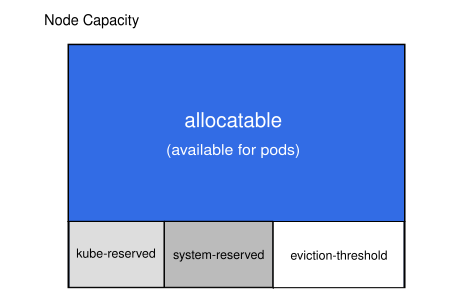
\includegraphics[width=0.7\textwidth]{resources/node-capacity.png}
	\captionof{figure}{Node resources: capacity and allocatable}
	\label{fig:test1}
\end{figure}

\subsubsection{The \co{PodDisruptionBudget} Object}
\label{section:Pod-disruption-budge}

Pods do not disappear until someone (a person or a controller) destroys them or
there is an unavoidable hardware or system software error.

The unavoidable cases are called \emph{involuntary disruptions} and include:
\begin{itemize}
	\tightlist
	\item A hardware failure of the physical machine backing the node.
	\item Cluster administrator deletes VM (instance) by mistake.
	\item Cloud provider or hypervisor failure makes VM disappear.
	\item A kernel panic.
	\item The node disappears from the cluster due to cluster network partition.
	\item Eviction of a Pod due to the node being out-of-resources.
\end{itemize}

All other cases are called \emph{voluntary disruptions}. These include both
actions initiated by the application owner and those initiated by a Cluster
Administrator. Typical voluntary disruptions include:

\begin{itemize}
	\tightlist
	\item Deleting the deployment or other controller that manages the Pod.
	\item Updating a deployment's Pod template causing a restart.
	\item Directly deleting a Pod.
	\item Draining a node for repair or upgrade.
	\item Draining a node from a cluster to scale the cluster down.
	\item Removing a Pod from a node to permit something else to fit on that
	      node.
\end{itemize}

A \texttt{PodDisruptionBudget} (PDB) limits the number of Pods of a replicated
application that are down simultaneously from voluntary disruptions. For
example, a web front end might want to ensure that the number of replicas
serving load never falls below a certain percentage of the total.

A PDB specifies the number of replicas that an application can tolerate having,
relative to how many it is intended to have. For example, a Deployment that has
a \texttt{.spec.replicas:\ 5} is supposed to have 5 Pods at any given time. If
its PDB allows for there to be 4 at a time, then the Eviction API will allow
voluntary disruption of one (but not two) Pods at a time.

Involuntary disruptions cannot be prevented by PDBs; however they do count
against the budget. Pods which are deleted or unavailable due to a rolling
upgrade to an application do count against the disruption budget.

\subsubsection{The \co{Deployment} Object}
\label{section:deployment}
A \co{Deployment} resource ensures that a specified number of Pod
\textit{replicas} are running at any time. In other words, a Deployment ensures
that a Pod or homogeneous set of Pods are always up and available. If there are
too many Pods, it will kill some. If there are too few, the Deployment will
start more.

\subsubsection{The \co{DaemonSet} Object}
\label{section:daemone-set}

A \co{DaemonSet} (DS) resource ensures that all Nodes run a copy of a Pod. As
nodes are added to the cluster, Pods are added to them. As nodes are removed
from the cluster, those Pods are garbage collected. Deleting a DaemonSet will
clean up the Pods it created.

\subsubsection{The \co{PersistentVolumeClaim} object}

A \co{PersistentVolumeClaim} (PVC, or equivalently referred to as ``claim'')) is
a request for storage by a user. Claims can request specific size and access
modes, e.g., they can be mounted \co{ReadWriteOnce}, \co{ReadOnlyMany} or
\co{ReadWriteMany}, etc.


\paragraph*{Phase}
The \textit{Phase} of a PVC can be one of the following:
\label{section:pvc-phase}
\begin{enumerate}
	\tightlist
	\item \texttt{Pending}: the PVC is not yet bound.
	\item \texttt{Bound}: the PVC is bound to a PV.
	\item \texttt{Lost}: the PVC lost its underlying PV. The claim was bound to
	      a  PV and this volume does not exist any longer and all data on it was
	      lost.
\end{enumerate}


\subsubsection{The \co{PersistentVolume} object}

A \co{PersistentVolume} (PV, or equivalently referred to as ``volume'') is a
piece of storage in the cluster that has been provisioned by an administrator or
dynamically provisioned using Storage Classes. It is a resource in the cluster.
PVs have a lifecycle independent of any individual Pod that uses the PV. This
\co{API} object captures the details of the implementation of the storage, be that
NFS, iSCSI, or a cloud-provider-specific storage system.

\begin{figure}[ht]
	\centering
	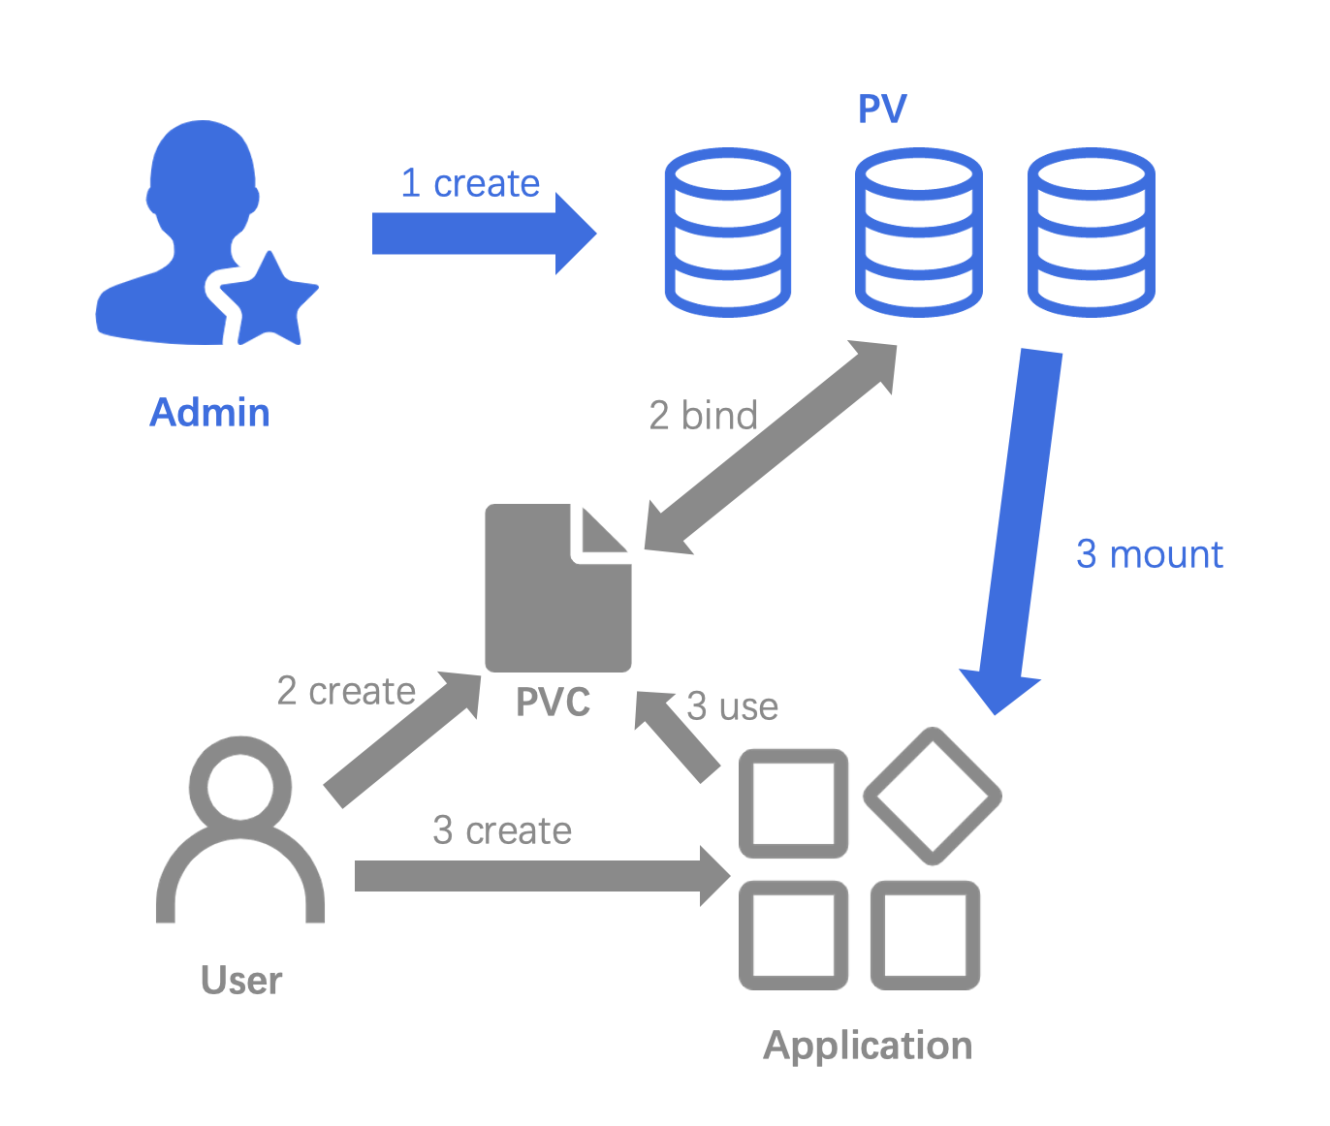
\includegraphics[width=0.6\textwidth]{resources/pvc-lifecycle.png}
	\caption{The lifecycle of a PVC and PV in the case of static provisioning}
\end{figure}

\paragraph*{Phase} A PV can be in one of the following phases:
\label{section:pv-phase}
\begin{itemize}
	\tightlist
	\item \texttt{Available}: the PV is not yet bound; it is available to be
	      matched to a PVC.
	\item \texttt{Bound}: the PV is bound to a PVC.
	\item \texttt{Released}: the PVs must be recycled before becoming available
	      again. This phase is used by the persistent volume claim binder to
	      signal to another process to reclaim the resource.
	\item \texttt{Failed}: the PV has failed to be correctly recycled or deleted
	      after being released from a claim.
\end{itemize}


\paragraph*{Binding}
PVCs are requests for storage resources; each PVC gets bound to a PV that
matches the PVC's requested storage amount and access modes. Each PV gets bound
to one PVC only, and vice versa. The binding between them is bidirectional.  A
PV will remain unbound till it is matched to a PVC. The binding is illustrated
in Figure \ref{figure:pvc-pv}.

\begin{figure}[ht]
	\centering
	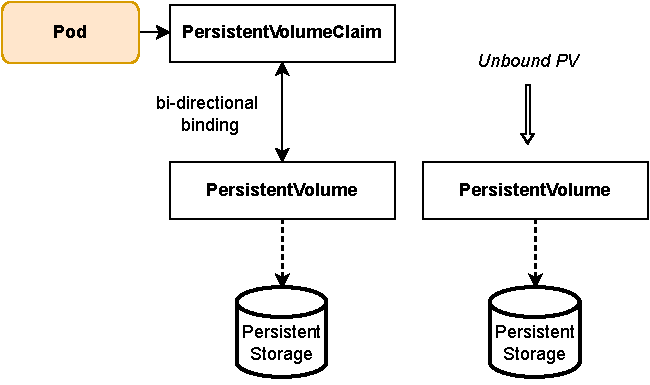
\includegraphics[width=0.8\textwidth]{resources/pvc-pv-binding.pdf}
	\caption{A Pod requests a volume using a PVC and the PVC gets bound to a PV. The PV object stores the details for the underlying persistent storage piece.}
	\label{figure:pvc-pv}
\end{figure}

The interaction between PVs and PVCs follows this lifecycle:
\begin{enumerate}
	\item \textbf{Provisioning}: There are two ways PVs may be provisioned:
	      statically or dynamically.
	      \begin{itemize}
		      \item \textbf{Statically}: A cluster administrator creates some
		            PVs. They carry the details of the actual storage, which is
		            available for use by cluster users. They exist in the
		            Kubernetes API and are available for consumption. \item
		            \textbf{Dynamically}: When none of the static PVs the
		      \item \textbf{Dynamically}: When none of the static PVs the
		            administrator created matches a user's
		            PersistentVolumeClaim, the storage system may try to
		            dynamically provision a volume for the PVC. This
		            provisioning relies on storage classes: the PVC must request
		            a storage class, and the administrator must have created and
		            configured that class for dynamic provisioning. Claims that
		            do not specify a storage class effectively disable dynamic
		            provisioning for themselves.
	      \end{itemize}
	\item \textbf{Binding}: A user creates a PersistentVolumeClaim with a
	      specific amount of storage requested and with certain access modes. A
	      control loop (the PersistentVolumeController) in the Kubernetes
	      control plane watches for new PVCs, finds a matching PV (if possible),
	      and binds them together. If a PV was dynamically provisioned for a new
	      PVC, the loop binds that PV to the PVC. Otherwise, the user will get
	      at least what they asked for, but the volume may be more than what was
	      requested. Once bound, PersistentVolumeClaim binds are exclusive,
	      regardless of how they were bound. A PVC to PV binding is a one-to-one
	      mapping, using a \co{ClaimRef} which is a bidirectional binding
	      between the PersistentVolume and the PersistentVolumeClaim. Claims
	      will remain unbound indefinitely if a matching volume does not exist.
	      Claims will be bound as matching volumes become available. For
	      example, a cluster provisioned with many 50Gi PVs would not match a
	      PVC requesting 100Gi. The PVC can be bound when a 100Gi PV is added to
	      the cluster.
	\item \textbf{Using}: Pods use claims as volumes. The cluster inspects the
	      claim to find the bound volume and mounts that volume for a Pod. For
	      volumes that support multiple access modes, the user specifies which
	      mode is desired when using their claim as a volume in a Pod. Once a
	      user has a claim and that claim is bound, the bound PV belongs to the
	      user for as long as they need it. Users access their claimed PVs by
	      including a \co{persistentVolumeClaim} section in a Pod's \co{volumes}
	      block.
\end{enumerate}

In the context of this thesis, a PVC will be also referred to as a
``\texttt{claim}''

\paragraph*{Node affinity}
\label{section:background-pv-node-affinity}

A PV can specify node affinity to define constraints that limit what nodes this
volume can be accessed from. The \co{nodeAffinity} field of the PV is a label
selector that matches nodes with the appropriate labels. Labels are key/value
pairs that are attached to objects.

The node affinity of a PV is used in the following way to indicate a volume is
local to a node:
\begin{enumerate}
	\tightlist
	\item The storage driver sets on each \texttt{Node} object a unique label.
	\item The storage driver sets the corresponding node affinity of the PV to
	      match only the unique label of the node.
\end{enumerate}

Listing ~\ref{listing:pv-affinity} presents a PV with node affinity that matches
node having the label \co{node:node-1}.

\lstinputlisting[label={listing:pv-affinity},language=yaml,caption={A PV with node affinity}]{code/node-affinity.yaml}

\subsubsection{The \co{StorageClass} Object}

A \co{StorageClass} is a Kubernetes resource that enables dynamic storage
provisioning. A StorageClass provides a way for administrators to describe the
``classes'' of storage they offer. The administrator configures the
StorageClass, which can then no longer be modified.

A storage class can specify a \co{volumeBindingMode}, which is either
\co{Immediate} or \co{WaitForFirstConsumer}:
\begin{itemize}
	\item  \co{Immediate}: Indicates that volume binding and dynamic
	      provisioning occur once the user creates the PersistentVolumeClaim.
	      For storage backends that are topology-constrained and not globally
	      accessible from all nodes in the cluster, PersistentVolumes will be
	      bound or provisioned without knowledge of the Pod's scheduling
	      requirements, possibly resulting in unschedulable Pods.
	\item \co{WaitForFirstConsumer}: The binding and provisioning of a
	      PersistentVolume will be delayed until a Pod using the
	      PersistentVolumeClaim is created. PersistentVolumes will be selected
	      or provisioned conforming to the topology that is specified by the
	      Pod's scheduling constraints.
\end{itemize}


\subsection{The Eviction API}
\label{section:background-eviction}

When deleting a resource on Kubernetes, the API server will put a
\co{deletionTimestamp} on the resource object. Unless there are any finalizers
on the object, the object will be removed from the API Server.

In the case of Pods, apart from the classic \co{DELETE} operation, Kubernetes
offers an extra API to initiate the deletion of the Pod: the \co{Eviction} API.
The main difference with the delete operation is that API-initiated evictions
respect the configured PodDisruptionBudgets and
\co{terminationGracePeriodSeconds}. So, if a user tries to \textit{evict} a Pod
and the corresponding PodDisruptionBudget does not allow the disruption of the
Pod, the Pod will not be deleted. Instead, issuing a classical \co{DELETE}
operation will remove the Pod, no matter what the PodDisruptionBudget specifies.

\subsection{The Cordon \& Drain Operations}
\label{section:cordon-drain}

The Kubernetes command-line tool, \co{kubectl}, allows a user to run commands
against Kubernetes clusters. The tool allows the complete management of the
cluster. Two essential operations used for the maintenance of the cluster are
the \textit{cordon} and the \textit{drain} operations.

\paragraph*{Cordon operation}
\textit{Cordon} is an operation offered by the \co{kubectl} CLI tool that marks
the node as \textit{unschedulable}. Marking a node as unschedulable prevents the
scheduler from placing new Pods onto that node but does not affect existing Pods
running on it. This is a preparatory step before a node reboot or other
maintenance.

The admin of the cluster can execute the cordon operation by running \co{kubectl
	cordon}. When cordoning a node, the tool adds the \textit{unschedulable
	taint} \footnote{Unschedulable taint:
	\co{node.kubernetes.io/unschedulable:NoSchedule}} on the node and also sets
	the \co{nodes.spec.unschedulable} field to \co{True}.

We will refer to the action of marking the node as unschedulable as
``\textit{cordoning the node}'' and the node as ``\textit{cordoned}''.

\paragraph*{Drain operation}

The \textit{drain} operation is used to remove workload from a node. It is run
in case the node needs maintenance, or it needs to be removed from a cluster.
The drain operation cordons the node to mark it as unschedulable, and evicts all
the Pods from the node.  Evictions allow the Pod's containers to terminate
gracefully and will respect the PodDisruptionBudgets the user has specified.

The admin of the cluster can execute the drain operation by running \co{kubectl
	drain}. If \co{kubectl drain} returns successfully, it indicates that all
	the Pods have been safely evicted (respecting the desired graceful
	termination period and the PodDisruptionBudget that is defined). It is then
	safe to bring down the node by powering down its physical machine or
	deleting its virtual machine if it runs on a cloud platform.

\section{Kubernetes Controllers}
In Kubernetes, controllers are control loops that watch the state of the
cluster, then make or request changes where needed. Each controller tries to
move the current cluster state closer to the desired state. A controller tracks
at least one Kubernetes resource type. These objects have a \co{spec} field
representing the desired state. The controllers for that resource are
responsible for making the current state come closer to that desired state.

In this section, we will describe some of the controller that play a significant
role in the storage system of Kubernetes.


\subsection{The PersistentVolume Controller}

The \co{PersistentVolumeController} is a controller that synchronizes
PersistentVolumeClaims and PersistentVolumes.  It binds PVs and PVCs and manages
their lifecycles. If the PVC references a StorageClass with static provisioning,
the control loop attempts to find a matching PV and then binds it to the PVC. In
the case of dynamic provisioning, as soon as the PV gets provisioned for the
PVC, the control loop binds them together.

\subsection{The AttachDetach Controller}

The \co{AttachDetach} controller manages volume attach and detach operations. It
looks for any Pods that get scheduled on a node and triggers the attach
operation, i.e., it creates a \co{VolumeAttachment} object to signal the
external attacher that it shall issue a \co{ControllerPublish} call to the CSI
driver. Similarly, when no Pods use a volume on a node, the controller executes
a detach operation: deletes the \co{VolumeAttachment} object to signal the external
attacher it shall issue a \co{ControllerUnpublish} request to the CSI driver.


\subsection{Kubernetes Admission Controllers}

An \textit{admission controller} is a piece of code that intercepts requests to
the Kubernetes API server prior to the persistence of the object but after the
request is authenticated and authorized. Admission controllers may be
\textit{validating}, \textit{mutating}, or both. Mutating controllers may modify
related objects to the requests they admit; validating controllers may not.

The admission control process proceeds in two phases. In the first phase, it
runs the mutating admission controllers. In the second phase, it runs the
validating admission controllers. If any controller in either phase rejects the
request, the entire request is rejected immediately and an error is returned to
the end-user.

Various admission controllers come compiled into the \co{kube-apiserver} binary,
and out of them, there are two controllers of particular interest, the
\co{MutatingAdmissionWebhook} and \co{ValidatingAdmissionWebhook}:
\begin{itemize}
      \tightlist
      \item \co{MutatingAdmissionWebhook}: This admission controller calls any
            mutating webhooks which match the request. Matching webhooks are called
            serially; each one may modify the object if desired.

      \item \co{ValidatingAdmissionWebhook}: This admission controller calls any
            validating webhooks which match the request. Matching webhooks are
            called in parallel; if any of them rejects the request, the request
            fails.
\end{itemize}

The admission controller phases are shown in Figure
~\ref{figure:admission-controller}.
\begin{figure}[ht]
      \centering
      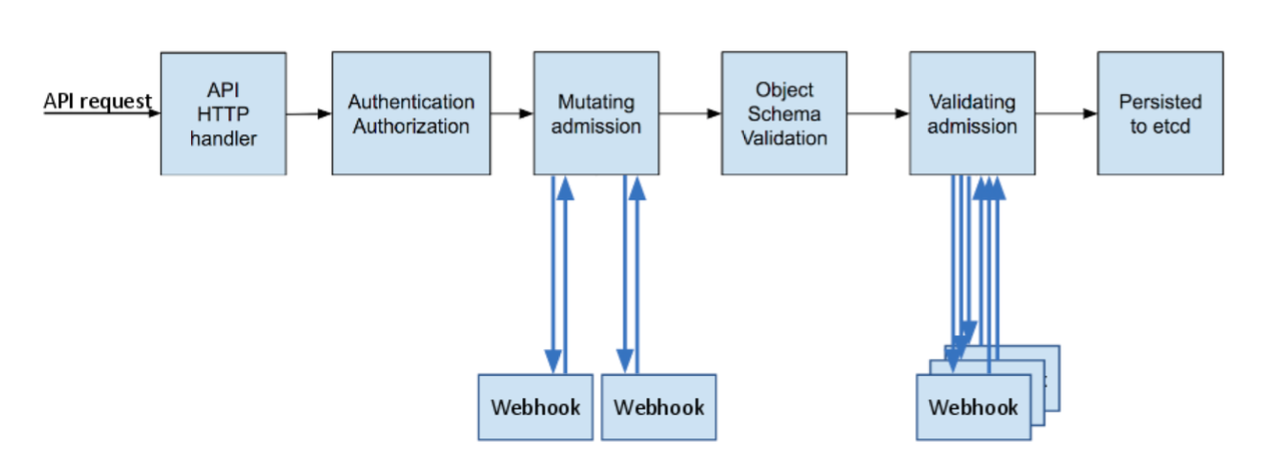
\includegraphics[width=\textwidth]{resources/admission-controller-phases.png}
      \caption{Admission controller phases}
      \label{figure:admission-controller}
\end{figure}

\section{Kubernetes Admission Webhooks}

Admission webhooks are HTTP callbacks that receive admission requests and do
something with them. Two types of admission webhooks can be defined:
\textit{validating admission} webhook and \textit{mutating admission} webhook.

Mutating admission webhooks are invoked first, and can modify objects sent to
the API server to enforce custom defaults. After all object modifications are
complete, and after the incoming object is validated by the API server,
validating admission webhooks are invoked and can reject requests to enforce
custom policies.The admin of the cluster can dynamically configure what
resources are subject to what admission webhooks via
\co{ValidatingWebhookConfiguration} or \co{MutatingWebhookConfiguration} API
objects.

\paragraph*{\co{MutatingWebhookConfiguration} Object}

Each \texttt{MutatingWebhookConfiguration} contains a list of webhooks,
specified at \co{webhooks} field. Each of the webhooks defined, may specify the
following fields:
\begin{itemize}
      \tightlist
      \item \texttt{rules}: A list of rules used to determine if a request to
            the API server should be sent to the webhook. Each rule specifies
            one or more operations, apiGroups, apiVersions, and resources, and a
            resource scope.
      \item  \texttt{failurePolicy}: Defines how unrecognized errors and timeout
            errors from the admission webhook are handled. Allowed values are
            \texttt{Ignore} or \texttt{Fail}.
      \item \texttt{namespaceSelector}:  Defines whether to run the webhook on a
            request for a namespaced resource (or a \texttt{Namespace} object) based
            on whether the namespace labels match the selector. If the object is a
            cluster scoped resource other than a Namespace, \texttt{namespaceSelector}
            has no effect.
\end{itemize}

\section{The Kubernetes Operator Pattern}
\label{section:operator-pattern}

A Kubernetes operator is a custom application-specific controller that extends
the functionality of the Kubernetes API to create, configure, and manage
instances of complex applications on behalf of a Kubernetes user. It builds upon
the fundamental Kubernetes resource and controller concepts but includes domain
or application-specific knowledge to automate the entire life cycle of the
software it manages. It uses \textit{custom resources} to manage applications
and their components. The user within a custom resource provides high-level
configuration and settings. The Kubernetes operator translates the high-level
directives into low-level actions based on best practices embedded within the
operator's logic.

A \co{CustomResourceDefinition} object (CRD) defines a custom resource and lists
out all the configurations available to users of the operator. The Kubernetes
API can handle custom resource definitions just like built-in objects, including
interaction via \co{kubectl} and inclusion in role-based access control (RBAC)
policies.

\begin{figure}[ht]
	\centering
	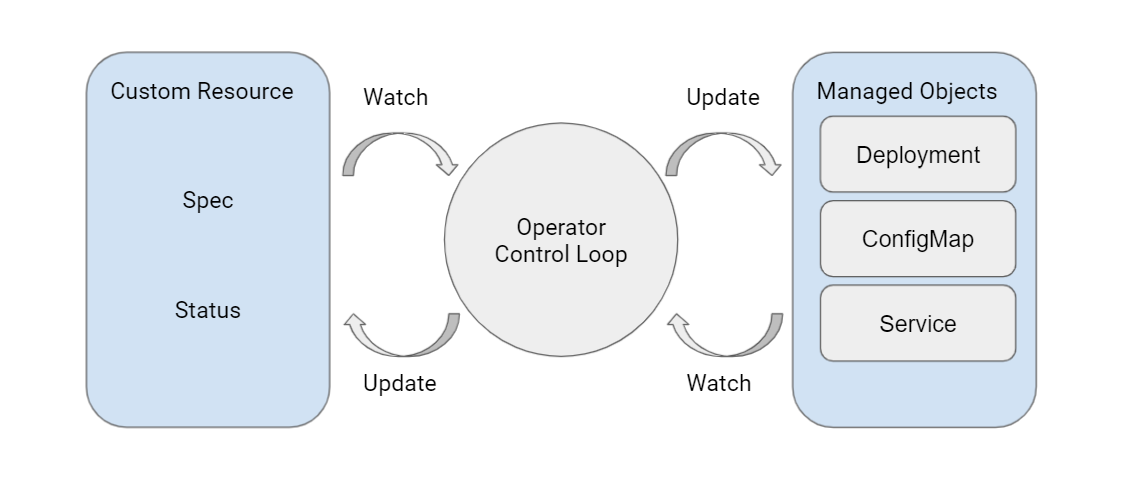
\includegraphics[width=0.8\textwidth]{resources/operator.png}
	\caption{The Kubernetes operator pattern}
\end{figure}

\section{Kubernetes Scheduler}
\RestyleAlgo{ruled}

Σε αυτήν την ενότητα, θα παρουσιάσουμε συνοπτικά τη τρέχουσα σχεδίαση του
Kubernetes Scheduler, θα επισημάνουμε τις ελλείψεις που υπάρχουν και θα
προτείνουμε βελτιώσεις που επιλύουν τους τρέχοντες περιορισμούς.

\subsection{To Πρόσθετο VolumeBinding}

Για λόγους συντομίας, στο ελληνικό τμήμα της διπλωματικής παρουσιάζουμε μόνο τη
σχεδίαση της \co{Filter} και της \co{PreBind}  φάσης του προσθέτου, καθώς
σχετίζεται άμεσα με τις προτεινόμενες επεκτάσεις. Για την αναλυτική παρουσίαση
των υπολοίπων φάσεων του προσθέτου, μπορείτε να ανατρέξετε στο αντίστοιχο
αγγλικό κεφάλαιο, στην ενότητα \ref{section:design-volume-binding}.

\subsection*{PreFilter Φάση}

\co{Filter}: αξιολογεί αν ένα Pod μπορεί να τοποθετηθεί σε έναν κόμβο, βάσει των
τόμων που ζητά, τόσο για τα δεσμευμένα όσο και για τα μη δεσμευμένα PVC:
\begin{itemize}
      \tightlist
      \item Για τα \textit{δεσμευμένα PVC}, ελέγχει ότι το PV του κάθε PVC είναι
            προσβάσιμο (βάσει τoy node affinity που φέρει) από τον εξεταζόμενο
            κόμβο.
      \item Για τα \textit{μη δεσμευμένα PVC}, προσπαθεί να βρει διαθέσιμα PVs
            που μπορούν να ικανοποιήσουν τις απαιτήσεις του PVC και που είναι
            προσβάσιμα (βάσει του node affinity τους) από τον εξεταζόμενο κόμβο.
            Τα PVCs για τα οποία δεν κατάφερε να βρει κατάλληλα PVs, θα τα
            αποκαλούμε εφεξής ``\textit{PVCs to provision}''.
      \item Για κάθε \textit{PVC to provision}, ελέγχει αν η \co{StorageClass}
            του PVC υποστηρίζει τη δυναμική παροχή και αν υπάρχει αρκετή
            χωρητικότητα αποθήκευσης προσβάσιμη από τον κόμβο. Εάν όχι, το Pod
            δεν μπορεί να ανατεθεί στον κόμβο. Αυτό είναι το βήμα όπου
            η χωρητικότητα αποθήκευσης λαμβάνεται υπόψη.

\end{itemize}

Η τρέχουσα υλοποίηση του χρονοδρομολογητή, ελέγχει αν υπάρχει αρκετή
χωρητικότητα για κάθε PVC to provision, καλώντας τη μέθοδο \co{hasEnough()} με
ένα μόνο PVC ως είσοδο. Ζητά από τον  API Server όλα τα αντικείμενα
\co{CSIStorageCapacity}. και ελέγχει αν κάποιο από αυτά ταιριάζει με το
\co{StorageClass} του PVC, είναι προσβάσιμο από τον εξεταζόμενο κόμβο και η
αναφερόμενη χωρητικότητα του αντικειμένου είναι μεγαλύτερη από τη ζητούμενη
χωρητικότητα του PVC. Εάν ένα τέτοιο CSIStorageCapacity υπάρχει, υπάρχει αρκετός
χώρος στον κόμβο για τη δυναμική παροχή τόμου για το εξεταζόμενο PVC.

Είναι σημαντικό να επισημάνουμε ότι δεν ελεγχει αν υπάρχει αποθηκευτικός χώρος
συνολικά για όλα τα PVCs, αλλά μόνο αν το κάθε PVC χωριστά χωράει σε έναν κόμβο.

\subsection*{PreBind Φάση}

Η φάση \co{PreBind} εκτελείται αφού ο χρονοδρομολογητής έχει επιλέξει έναν κόμβο
για  το Pod.

Για κάθε ένα από τα \textit{μη δεσμευμένα PVC} που το πρόσθετο βρήκε ένα
κατάλληλο PV κατά τη διάρκεια της φάσης \co{Filter}, θα ενημερώσει τον API
Server με τη δέσμευση, δηλαδή, θα ενημερώσει το αντίστοιχο PV ώστε να δείχνει
στο PVC, και στη συνέχεια, ο ελεγκτής Kubernetes PersistentVolume θα ολοκληρώσει
την αμφίδρομη δέσμευση.

Για κάθε ένα από τα \textit{PVCs to provision}, θα ενημερώσει τα αντίστοιχα PVCs
στον API Server με το  ``selected node annotation'' \footnote{Το selected node
annotation: \co{volume.kubernetes.io/selected-node}} για να σηματοδοτήσει στον
\en{external provisioner} ότι ένας τόμος για το PVC πρέπει να δημιουργηθεί δυναμικά
σε ένα τμήμα τοπολογίας που είναι προσβάσιμο από τον κόμβο που υποδεικνύει η
σημείωση. 

Στη συνέχεια, το πρόσθετο θα κάνει poll τον API Server έως ότου όλα τα PVCs
δεσμευτούν  PVs. Εάν το selected node annotation κάποιου PVC to provision
αφαιρεθεί, θα ακυρώσει την τρέχουσα προσπάθεια χρονοδρομολόγησης και θα
καλέσει τα πρόσθετα \co{Unreserve}.Η αφαίρεση του annotation είναι ένας
μηχανισμός με τον οποίο ο external provisioner ουσιαστικά ειδοποιεί τον
χρονοδρομολογητή ότι απέτυχε η παροχή του τόμου και θα πρέπει να δοκιμάσει ξανά,
ενδεχομένως σε άλλον κόμβο.


\subsection{Ελλείψεις \& Προτεινόμενες Επεκτάσεις}

Σύμφωνα με την προηγούμενη ανάλυση των αλγορίθμων, ο τρέχων σχεδιασμός του
Kubernetes Scheduler έχει τους ακόλουθους περιορισμούς:

\begin{enumerate}
      \item Η μέθοδος \texttt{Filter} του πρόσθετου VolumeBinding χρησιμοποιεί
            τα αντικείμενα \en{CSIStorageCapacity} του Kubernetes API για να
            αντλήσει πληροφορίες για τον διαθέσιμο αποθηκευτικό χώρο. Αυτό το
            αντικείμενο API έγινε beta στην έκδοση Kubernetes 1.21 και ήταν σε
            κατάσταση alpha σε προηγούμενες εκδόσεις. Οι κύριοι πάροχοι
            υπηρεσιών νέφους δεν ενεργοποιούν τα χαρακτηριστικά σε κατάσταση
            alpha στις υπηρεσίες τους. Ως αποτέλεσμα, τα CSIStorageCapacity
            αντικείμενα δεν είναι ενεργοποιημένα σε συστοιχίες που εκτελούν
            εκδόσεις προγενέστερες της 1.21 στους περισσότερους παρόχους cloud.
            Αυτό είναι ένα σημαντικό πρόβλημα, δεδομένου ότι πολλές επιχειρήσεις
            (συμπεριλαμβανομένων των πελατών μας) δεν τρέχουν τις τελευταίες
            εκδόσεις του Kubernetes για λόγους σταθερότητας. Στη δική μας
            περίπτωση, οι πελάτες μας εκτελούν συστοιχίες Kubernetes 1.19 και
            1.20 και χρειάζονταν τη δυνατότητα χρονοδρομολόγησης Pods με εξέταση
            της τοπικής αποθήκευσης.
      \item Η τρέχουσα σχεδιαστική λογική της φάσης \co{Filter} του πρόσθετου
            \co{VolumeBinding} δεν λαμβάνει υπόψη της τον αποθηκευτικό χώρο που
            απαιτείται για την παροχή πολλαπλών PVC ενός Pod. Αντ' αυτού,
            ελέγχει αν κάθε μεμονωμένο PVC μπορεί να δημιουργηθεί στον
            αποθηκευτικό χώρο που είναι προσβάσιμος από τον κόμβο, χωρίς να
            διασφαλίζει ότι υπάρχει αρκετός χώρος για όλα αυτά ταυτόχρονα. Αυτό
            είναι ένα κρίσιμο πρόβλημα: σε περίπτωση που ένα Pod αναφέρεται σε
            πολλαπλά μη δεσμευμένα PVC και δεν υπάρχει αρκετός χώρος για όλα
            αυτά, ένα από αυτά γίνει provision και η παροχή των υπολοίπων θα
            αποτύχει, τότε όλες οι μελλοντικές αποφάσεις χρονοδρομολόγησης θα
            περιορίζονται από το ήδη δημιουργημένο τόμο και το Pod θα κολλήσει.
\end{enumerate}

Δεδομένου ότι ο σχεδιασμός του upstream έρχεται με τους προαναφερθέντες
περιορισμούς, προτείνουμε να επεκτείνουμε τον Kubernetes Scheduler και να
εγκαταστήσουμε τον επεκταμένο χρονοδρομολογητή στη συστοιχία. Ο προτεινόμενος
σχεδιασμός μπορεί να χωριστεί στα ακόλουθα μέρη:

% TODO: enumerate or itemize?
\begin{enumerate}
      \tightlist
      \item Επέκταση του Rok CSI Node του οδηγού αποθήκευσης, ώστε να
            αναφέρει τη διαθέσιμη χωρητικότητα κάθε κόμβου ως annotation στο
            αντίστοιχο αντικείμενο \texttt{Node} του Kubernetes.
      \item Επέκταση του Rok CSI Controller του οδηγού αποθήκευσης
            ώστε να απαντά με κατάλληλο σφάλμα στην κλήση \co{CreateVolume} όταν
            η εναπομένουσα χωρητικότητα για την παροχή του τόμου είναι
            ανεπαρκής.
      \item Επέκταση του πρόσθετου VolumeBinding του Kubernetes Scheduler ώστε
            να ελέγχει αν πολλαπλοί τόμοι ενός Pod χωρούν σε έναν κόμβο,
            συγκρίνοντας τη συνολική τους απαίτηση σε χωρητικότητα με την
            αναφερθείσα διαθέσιμη χωρητικότητα.
      \item Εγκατάσταση του επεκταμένου χρονοδρομολογητή στη συστοιχία.
      \item Ανάπτυξη και εγκατάσταση ενός  webhook που θα μεταλλάσσει τα Pods
            ώστε να χρησιμοποιούν τον επεκταμένο χρονοδρομολογητή.
\end{enumerate}

\subsubsection{Επέκταση του Rok CSI Node}

Δεδομένου ότι τα αντικείμενα \co{CSIStorageCapacity} δεν μπορούν να γίνουν
back-port σε προηγούμενες εκδόσεις του Kubernetes και, επίσης, η προσθήκη ενός
παρόμοιου Custom Resource θα απαιτούσε αρκετή προσπάθεια άνευ αιτίας,
αποφασίζουμε να αναφέρουμε τη χωρητικότητα κάθε κόμβου ως annotation στο
αντίστοιχο αντικείμενο Node. Το annotation, το οποίο αποκαλούμε ``annotation
χωρητικότητας'' θα είναι της μορφής
\co{rok.arrikto.com/capacity:<free-storage-bytes>}.

Το πρόσθετο Rok CSI Node του οδηγού αποθήκευσης που εκτελείται σε κάθε κόμβο της
συστοιχίας υπολογίζει περιοδικά τον διαθέσιμο αποθηκευτικό χώρο και ενημερώνει
το annotation χωρητικότητας. Δίνει εντολές στο Logical Volume Manager (LVM) του
κόμβου για να μάθει τον ελεύθερο χώρο του Rok Volume Group και ενημερώνει το
αντίστοιχο \co{Node} αντικείμενο με την τιμή της διαθέσιμης χωρητικότητας.

\subsubsection{Επέκταση του Rok CSI Controler}

Επεκτείνουμε το πρόσθετο Rok CSI Controller του οδηγού αποθήκευσης ώστε να
επιστρέφει το status  code \co{GRPCResourceExhausted} ως απάντηση στην κλήση
\co{CreateVolume} του external provisioner όταν η παροχή ενός τόμου αποτυγχάνει
λόγω ανεπαρκούς χωρητικότητας αποθήκευσης.

\subsubsection{Επέκταση του VolumeBinding Plugin}
\label{section:gr-volume-plugin-extensions}

Προτείνουμε την επέκταση της \co{Filter} μεθόδου του πρόσθετου
\co{VolumeBidning} ως εξής:
\begin{enumerate}
      \tightlist
      \item Κατά τον έλεγχο των PVCs του Pod που χρειάζονται να δημιουργηθούν
            δυναμικά (provision) (μέθοδος \co{checkVolumeProvisions()}), να
            επιλέγει όλα τα Rok PVCs
            \footnote{PVCs provisioned by the \co{rok.arrikto.com}
                  provisioner.} (εφεξής αναφέρονται ως ``\\textit{Rok claims to
                  provision}'') και να ελέγχει αν υπάρχει αρκετή χωρητικότητα
                  για το συνολικό αποθηκευτικό χώρο που ζητούν.
      \item Να ελέγχει αν υπάρχει αρκετή χωρητικότητα για τα Rok claims to
            provision ως εξής:
            \begin{enumerate}
                  \tightlist
                  \item Να υπολογίζει τη συνολική χωρητικότητα που ζητείται
                        αθροίζοντας τα αιτήματά τους.
                  \item Να ελέγχει  αν ο εξεταζόμενος κόμβος διαθέτει annotation
                        χωρητικότητας του Rok \footnote{Το annotation
                        χωρητικότητας του Rok:
                        \texttt{rok.arrikto.com/capacity}} .
                  \item Αν to annotation \textit{δεν υπάρχει}, ή αν υπάρχει αλλά
                        δεν είναι έγκυρος ακέραιος αριθμός, τα Rok claims to
                        provision δεν μπορούν να δημιουργηθούν στον κόμβο. Η
                        απουσία της σημείωσης υποδεικνύει ότι το πρόγραμμα
                        οδήγησης Rok CSI δεν εκτελείται στον κόμβο.
                  \item Εάν υπάρχει το annotation χωρητικότητας, να ελέγχει αν η
                        αναφερόμενη διαθέσιμη χωρητικότητα είναι μεγαλύτερη ή
                        ίση με τη συνολική χωρητικότητα που ζητούν τα Rok claims
                        to provision. Εάν δεν ισχύει η συνθήκη, δεν υπάρχει
                        αρκετή χωρητικότητα, και τα Rok claims to provision δεν
                        μπορούν να δημιουργηθούν στον κόμβο,  οπότε και το Pod
                        δεν μπορεί να προγραμματιστεί στον κόμβο.
            \end{enumerate}
      \item Διατηρούμε της συμβατότητα προς τα πίσω με τη μη τροποποίηση του
            χειρισμού των  PVCs που δεν ζητούν αποθηκευτικό χώρο από την κλάση
            αποθήκευσης Rok. Ο σχεδιασμός μας, διαχωρίζει τα PVCs σε τοπικά Rok
            PVCs και μη Rok PVCs, και επεκτείνει μονάχα τον τρόπο χειρισμού
            μονάχα για τα Rok PVCs. Τα PVC που παρέχονται από άλλους παρόχους
            αποθήκευσης δεν θα επηρεαστούν από τις αλλαγές μας.
\end{enumerate}

% transl: επιπεδο ελέγχου


\subsubsection{Εγκατάσταση του Rok Scheduler}

Ο \co{kube-cheduler} εκτελείται από προεπιλογή σε κάθε πάροχο νέφους ως μέρος
του επιπέδου ελέγχου του Kubernetes και είναι ο προεπιλεγμένος χρονοδρομολογητής
που χρησιμοποιείται για τη χρονοδρομολόγηση των Pods. Οι πάροχοι νέφους
αποκρύπτουν το επίπεδο ελέγχου από τον τελικό χρήστη των υπηρεσιών τους, οπότε
δεν υπάρχει δυνατότητα αντικατάστασης και παραμετροποίησης του εκτελούμενου
χρονοδρομολογητή.

Ως συνέπεια αυτού του περιορισμού, εγκαθιστούμε στη συστοιχία --παράλληλα με τον
προεπιλεγμένο χρονοδρομολογητή--  τον δικό μας χρονοδρομολογητή, που εκτελεί το
επεκταμένο  VolumeBinding πρόσθετο.  Εφεξής θα αναφερόμαστε στον δικό μας
επεκταμένο χρονοδρομολογητή ως ``\textit{Rok Scheduler}''.

\subsubsection{Εγκατάσταση του Rok Scheduler Webhook}

Δεδομένου ότι εγκαθιστούμε τον Rok Scheduler χωρίς να αντικαταστήσουμε το
προεπιλεγμένο Kubernetes Scheduler της συστοιχίας, κάθε Pod πρέπει να καθορίζει
ποιος scheduler θα το χρονοδρομολογήσει ορίζοντας το πεδίο
\co{spec.schedulerName}. Εάν το πεδίο δεν έχει οριστεί, ο προεπιλεγμένος
χρονοδρομολογητής χρησιμοποιείται.

Σίγουρα δεν θέλουμε κάθε χρήστης να ορίζει χειροκίνητα το όνομα του scheduler
στο το Pod - αυτό θα επέτρεπε στους χρήστες να παρακάμψουν την πολιτική
χρονοδρομολόγησης που έχουμε ορίσει, είναι επιρρεπές σε σφάλματα και είναι μια
κουραστική διαδικασία. Χρειαζόμαστε έναν αυτόματο τρόπο για να το πετύχουμε
αυτό. Η λύση για την αυτοματοποίηση της εργασίας, είναι ένα mutating webhook.

Εγκαθιστούμε ένα μεταλλασσόμενο webhook στη συστοιχία, το οποίο στο εξής θα
αναφέρεται ως ``\textit{Rok Scheduler webhook}'', το οποίο δέχεται τα πρόσφατα
δημιουργηθέντα Pods σε συγκεκριμένα namespaces της συστοιχίας και τα
μεταλλάσσει προσθέτοντας το όνομα του Rok Scheduler στο πεδίο
\co{spec.schedulerName}.
\section{Kubernetes Cluster Autoscaler}
\label{section:autoscaler}
\RestyleAlgo{ruled0}

In this section, we are going to expose the design of the Cluster Autoscaler
(Autoscaler), describe its main principles of operation, identify its
limitations and propose extensions that will enable its seamless operation with
local persistent volumes.


\subsection{Fundamental terms}

Before we describe the algorithms of operations of the Autoscaler, it is
essential to understand some fundamental structures and terminology it uses.

\subsubsection{The Node Group Abstraction}

The Autoscaler uses the abstraction of a ``\textit{node group}''. A node group
is not an actual Kubernetes resource but rather an abstraction for a group of
nodes within a cluster. The Autoscaler expects that nodes found within a single
node group have the same resources (CPU, memory, storage) and share several
common properties such as labels and taints. However, they can still
differentiate in some details, e.g., they may consist of more than one
availability zone.

Each node group has the following important properties:
\begin{itemize}
      \tightlist
      \item \co{minSize}:minimum size of the node group.
      \item  \co{maxSize}: maximum size of the node group.
      \item  \co{targetSize}: the target size of the node group.
\end{itemize}

% TODO: Diagram TODO: PVC PV term TODO: All figures dots or not

\subsubsection{The \texttt{CloudProvider} Interface}

The Autoscaler operates with various cloud providers, e.g., GCE, AWS. To achieve
this, it specifies two important interfaces that each cloud provider that aims
to integrate its services with the Autoscaler must implement:
\begin{itemize}
      \tightlist
      \item The \co{CloudProvider} interface:  it contains configuration info
            and functions for interacting with the cloud provider.
      \item The \co{NodeGroup} interface: it contains configuration info and
            functions to control a node group.
\end{itemize}

The \co{NodeGroup} interface builds upon the node group abstraction. Each cloud
provider may choose its interpretation of what is a node group on its service,
as long as it conforms with the abstraction's definition.

For example, in the case of AWS EKS, the implementation of the \co{NodeGroup}
interface maps each node group to an AWS Auto Scaling Group (ASG). An Auto
Scaling group contains a collection of Amazon EC2 instances that are treated as
a logical grouping for automatic scaling and management purposes. An EC2
instance is a virtual server in Amazon Web Services terminology. A cluster
administrator configures the Auto Scaling groups of the EKS cluster and sets
their \co{minSize}, \co{maxSize} accordingly. The Autoscaler interacts with the
AWS cloud provider through the \co{CloudProvider} interface, which (the
CloudProvider interface) lists the configured Auto Scaling groups and maps each
of them to a node group. Only the \co{CloudProvider} interface knows about ASGs;
the rest components of the Autoscaler are unaware of the underlying
implementation and only see node groups.


\subsubsection{The \texttt{ClusterSnapshot} Interface}

The Autoscaler runs simulations on the cluster to make decisions. It takes a
snapshot of the current cluster, adds or removes nodes in the snapshot, and
simulates the scheduling decisions on the modified snapshot. A cluster snapshot
contains a fixed view of the cluster's nodes and the Pods that run on each node.
The \co{ClusterSnapshot} interface describes methods for taking a snapshot of
the cluster nodes and their Pods.

Note that the cluster's PVCs and PVs are not contained in the snapshot. Instead,
they are fetched from the API Server by the VolumeBinding plugin when the
\co{PredicateChecker} checks if a Pod can be placed on a node. We will explain
more about this later on.

\subsubsection{The \texttt{PredicateChecker} interface}

The Autoscaler defines the \co{PredicateChecker} interface, which offers methods
to check whether all required predicates pass for a given Pod and node.

A Predicate is equivalent to a \co{Filter} plugin (see section
\ref{section:background_scheduling_framework}) and it is used to filter out
nodes that can not run a Pod.

These are the methods of the interface:
\begin{itemize}
      \tightlist
      \item \co{CheckPredicates()}: checks if the given Pod can be placed on the
            given node.
      \item \co{FitsAnyNode()}: checks if the given Pod can be placed on any of
            the given nodes.
      \item \co{FitsAnyNodeMatching()}: checks if the given Pod can be placed on
            any of the given nodes matching the provided function.
\end{itemize}


The Autoscaler implements this interface. The implementation is called
\co{SchedulerBasedPredicateChecker} and leverages the Kubernetes Scheduler code.
In particular, the Autoscaler imports the code of the Kubernetes Scheduler and
constructs a list of predicates from the \co{Filter} plugins of the Scheduler.
The Autoscaler uses the \co{SchedulerBasedPredicateChecker} in its simulations
to determine whether a Pod can be placed on a node or not. The methods of the
interface it implements follow this basic flow:
\begin{enumerate}
      \tightlist
      \item Create a new scheduler \co{CycleState}.
      \item Run the \co{preFilter} method of all the plugins. Note that in the
            case of the VolumeBinding plugin, this step fetches the PVCs and PVs
            of the Pod from the API Server and stores them in the
            \co{CycleState}.
      \item Runs all the \co{Filter} plugins to determine if the Pod can be
            placed on the node.
\end{enumerate}

At this point, we shall highlight the fact that the Autoscaler imports the code
of the Kubernetes Scheduler and uses the \co{Filter} plugins it provides in the
\co{SchedulerBasedPredicateChecker} to run a simulation. However, it
\textbf{never} interacts with the live instance of the Kubernetes Scheduler that
runs on the cluster.

\subsubsection{The \texttt{Estimator} \& \texttt{Strategy} Interfaces}

The Autoscaler specifies two interfaces that are used in the scale-up procedure:
\begin{itemize}
      \tightlist
      \item \co{Estimator}: interface for calculating the number of nodes of a
            given type needed to schedule Pods.
      \item \co{Strategy}: interface for selecting the best option to scale up.
\end{itemize}


The estimator currently used by the Autoscaler is \co{BinPackingNodeEstimator}.
This estimator implements the First Fit Decreasing bin packing approximation
algorithm.

%TODO: Bin packing

\subsubsection{Template Nodes}
\label{section:design-template}

As we have explained, the Autoscaler assumes that every node in a node group
will have the same resources (CPU, memory, storage) and labels. It constructs a
template node for each node group to add it to the cluster snapshot and run its
simulations. As the name suggests, a template node represents the details of a
new node of the given node group. A template node is a \co{NodeInfo} struct and
contains the details of a real \co{Node} object and information about the DaemonSet
Pods that would run on the node if it was an actual node in the cluster. The
Autoscaler tries to build a template node of a node group as follows:

\begin{enumerate}
      \tightlist
      \item First, look for a ready and schedulable node of the node group in
            the cluster and use it to generate the template.
      \item If the previous step failed, look for a template in the Cluster
            Autoscaler's cache.
      \item If the previous step failed, call the cloud provider's compiled
            plugin to generate a template for the given node group.
      \item If the previous step failed, look for any unready or unschedulable
            node of the given node group in the cluster and use it to generate
            the template.
\end{enumerate}


The constructed template nodes are \textit{sanitized}: the sanitization is a
mechanism that removes irrelevant or undesired details from the constructed node
template, such as the name of the node, specific labels, etc.

The complete algorithm for template node creation is shown in
Algorithm~\ref{alg:template} and the algorithm for the node template
sanitization in Algorithm~\ref{alg:sanitize-template}.


\begin{algorithm}[H]
    \caption{Cluster Autoscaler: GetNodeInfoForGroup() method}\label{alg:template}
    \KwIn{node group: A NodeGroup struct.}
    \KwOut{A template node for the Node Group (NodeInfo struct).}
    \begin{enumerate}[leftmargin=0.5cm]
        \tightlist
        \item \If{a ready and schedulable node of the node group exists
                  in the cluster}{
                  \begin{enumerate}
                      \tightlist
                      \item Build the template from that node.
                      \item Store the template in the template's cache.
                      \item Return the template.
                  \end{enumerate}
              }
        \item \If{a template node for the node group exists in the Autoscaler's cache}{
                  \begin{enumerate}
                      \tightlist
                      \item Return the cached template node.
                  \end{enumerate}
              }
        \item Call \co{TemplateNodeInfo()} of the \co{NodeGroup} interface to
              get the cloud provider defined template for the node group.
        \item \If{the \co{TemplateNodeInfo()} generated the template successfully}{
                  \begin{enumerate}
                      \tightlist
                      \item Return the template.
                  \end{enumerate}
              }
        \item \If{an unready or unschedulable node of the node group exists
                  in the cluster}{
                  \begin{enumerate}
                      \tightlist
                      \item Build the template from that node.
                      \item Return the template.
                  \end{enumerate}
              }
        \item
              Return error, the template node could not be constructed.
    \end{enumerate}
\end{algorithm}
\clearpage
\begin{algorithm}[H]
\caption{Cluster Autoscaler: sanitizeNodeInfo() method}\label{alg:sanitize-template}
\KwIn{\co{node}: A template node (\co{NodeInfo} struct)}
\KwOut{A sanitized template node (\co{NodeInfo} struct).}
\begin{enumerate}
    \tightlist
    \item \co{nodeName} \lar \co{``template-node-for-<nodegroup-name>-<random-suf>''}.
    \item Set the \co{kubernetes.io/hostname} label of the node to \co{nodeName}
    \item Remove the following taints of the node:
      \begin{itemize}
        \tightlist
        \item \co{ToBeDeletedByClusterAutoscaler}
        \item \co{DeletionCandidateOfClusterAutoscaler}
        \item any taints that indicate the node's condition, e.g,
          \co{node.kubernetes.io/not-ready}
      \item taints starting with the \co{ignore-taint.cluster-autoscaler.kubernetes.io/} prefix.
      \end{itemize}
    \item Remove any taints of the node, as specified by the \co{--ignore-taints} flag of the Cluster Autoscaler.
    \item Return the sanitized node.
\end{enumerate}
\end{algorithm}

\subsubsection{Node Utilization}

As for scale-down, the Autoscaler acts based on a metric called the utilization
of a node; it calculates this metric using the \emph{resource requests} of the
Pods that run on the node instead of any actual (live) resource metrics.

Each Kubernetes node may have multiple resources, such as CPU, memory, etc. The
cluster Autoscaler computes the utilization of every node in the cluster. For a
given resource and node, the utilization is the ratio of the total resource
requests from the Pods running on the node over the resource allocatable of the
node. The utilization is a float number ranging from 0 to 1, where 1 indicates
full utilization and 0 no utilization.

For example, the CPU utilization is defined as:
\[ node\_cpu\_utilization  =  \frac{total\ CPU\ requests\ of\ Pods\ running\ on\
            the\ node }{ allocatable\ cpu\ of\ the\ node} \]

The steps for calculating the utilization of a node are shown in
Algorithm~\ref{alg:utilization}.

\begin{algorithm}[H]
\SetEndCharOfAlgoLine{.}
\caption{Cluster Autoscaler: CalculateUtilization() method}\label{alg:utilization}
    \KwIn{\co{node}: A Node API object
    \\ \co{pods}: the Pods running on the node
    \\ \co{resource}: a specific resource type, e.g, cpu, memory, etc
    }
    \KwOut{The utilization of node for a given resource}
    \begin{enumerate}[leftmargin=0.5cm]
        \tightlist
        \item  Get the node allocatable resource from the \co{Node} object:\\ \texttt{nodeAllocatable} \(\leftarrow\) \texttt{node.Status.Allocatable[resource]}.
        \item \lIf{nodeAllocatable == 0}{\Return 0}
        \item Initialize: \texttt{daemonSetRequests} \lar 0, \texttt{podRequest \lar 0}.
        \item Calculate the Pods' total resource requests. For each \co{pod} in \co{pods}: 
            \begin{enumerate}
            \tightlist
            \item \texttt{request} \lar  Calculate the resource request of the Pod by summing the
                \texttt{container.Resources.Requests{[}resourceName{]}} of each container of the
                \co{pod}.
            \item \lIf{Autoscaler is configured to ignore DaemonSet
                Pods in node utilization AND the Pod is a
                DaemonSet Pod}{
                \texttt{daemonSetRequests+= request}}
            \item \lIf {the Pod is long terminating}{continue to next Pod}
            \item \texttt{podRequest += request}.
            \end{enumerate}
    \item Calculate the utilization: \[ utilization =  \frac{podRequest - daemonSetRequests}{ nodeAllocatable - daemonSetRequests} \]
    \item \Return{utilization} 

    \end{enumerate}
\end{algorithm}
% TODO: Mirror long terminating 



\subsection{The Main Loop}
The Autoscaler runs continuously a loop, called the \textit{main loop}, which
executes two basic operations on the cluster:

\begin{itemize}
      \tightlist
      \item \textit{Scale-up}: adding new nodes to cluster to help unschedulable
            Pods.
      \item \textit{Scale-down}: removing unneeded nodes from a cluster.
\end{itemize}

The steps of the Autoscaler's main loop are shown in
Algorithm~\ref{alg:template}.

\clearpage
\begin{algorithm}[H]
  \caption{Cluster Autoscaler: The main loop - RunOnce() method}\label{alg:autoscaler-main-loop}
  \begin{enumerate}[leftmargin=0cm]
    \tightlist
    \item
          \texttt{unschedulablePods} \lar Select Pods that do not have \texttt{spec.nodeName} set.
    \item
          \texttt{scheduledPods} \lar Select Pods that have \co{spec.nodeName} set.
    \item
          \texttt{allNodes} \lar List all the nodes of the cluster, by calling \co{ObtainNodesList()}.
    \item
          \texttt{readyNodes} \lar List the Ready nodes of the cluster, by calling \co{ObtainNodesList()}.

    \item
          \co{nodeGroups} \lar List the registered node groups of the cluster from the cloud provider.
    \item
          Take a snapshot of the cluster.
    \item
          For every node group in \co{nodeGroups}, generate its template node.
    \item For each node group in \co{nodeGroups} calculate the number of
          upcoming nodes (nodes that the Autoscaler has asked to be added but
          are not yet in the cluster) and add the same number of the node
          group's template nodes in the cluster snapshot.
    \item
          Run a scheduling simulation with the current cluster snapshot to determine if any of the \texttt{unschedulablePods} can be scheduled on the upcoming nodes.
    \item \lIf{any Pod in \co{unschedulablePods} is considered as schedulable in
            the simulation}{disable the scale-down for the current loop}
    \item \co{unschedulablePodsToHelp} \lar Pods from \co{unschedulablePods} that remained unschedulable in the simulation.
    \item \lIf{\co{unschedulablePodsToHelp} is empty}{do not scale-up}
    \item
          Else, try to scale-up, by calling \co{ScaleUp()}.
    \item
          \lIf{no scale-up was attempted}{proceed with the scale-down evaluation}
  \end{enumerate}
\end{algorithm}

\clearpage
\begin{figure}[H]
      \centering
      \makebox[\textwidth][c]{
            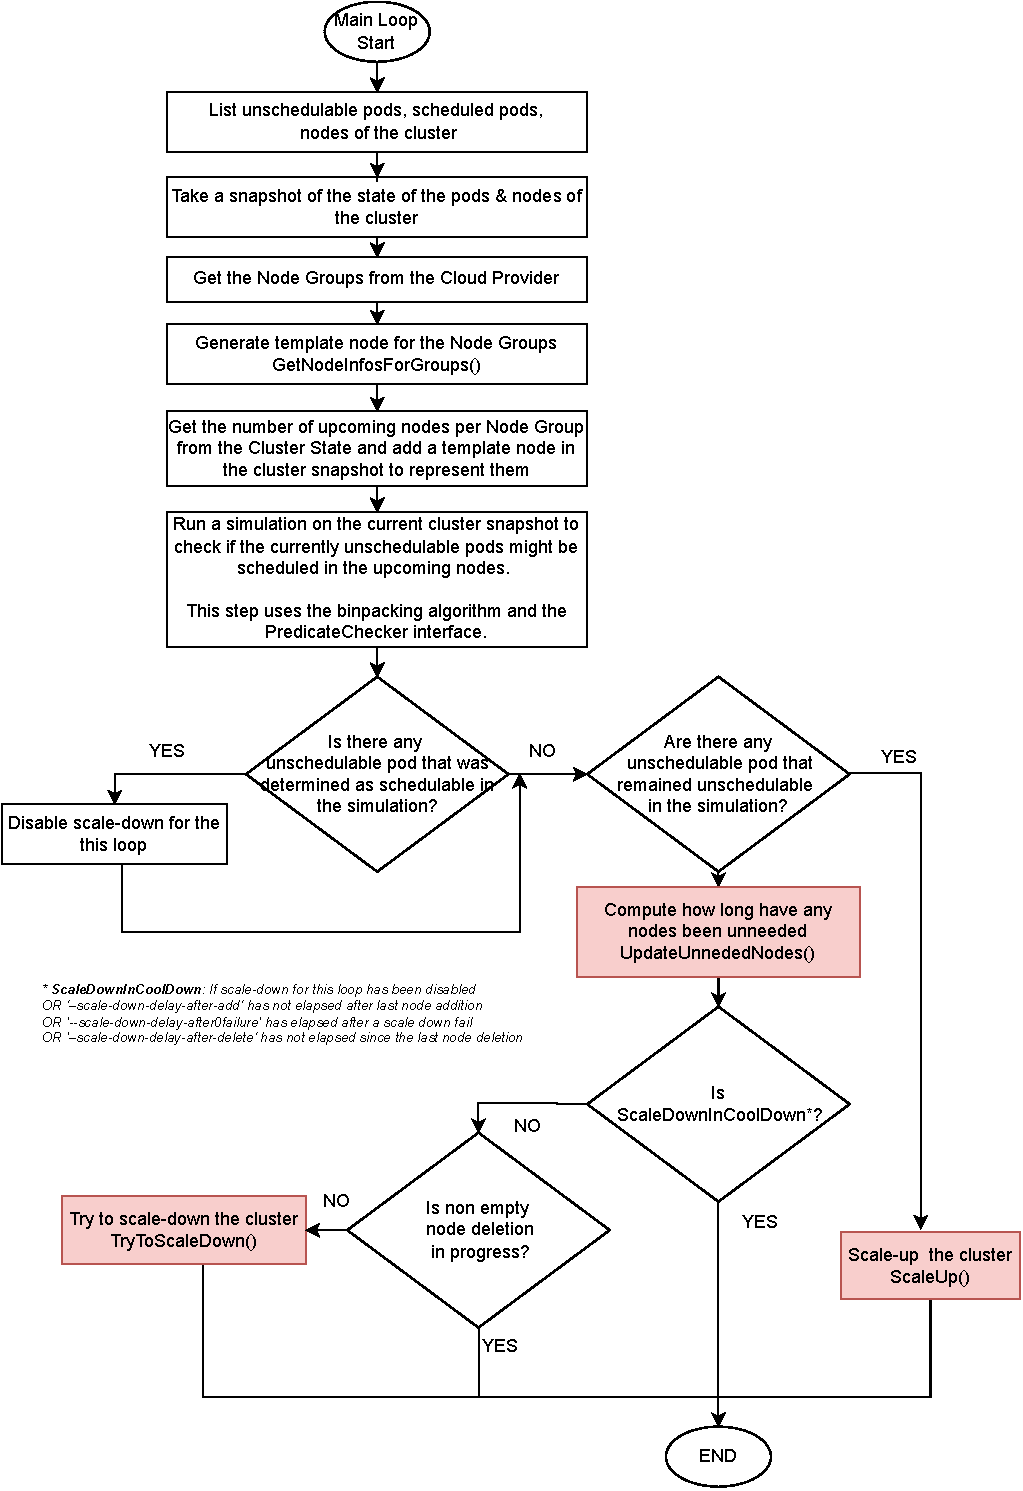
\includegraphics[width=\textwidth]{resources/autoscaler-main-loop.pdf}
      }
      \caption{Cluster Autoscaler:The main loop}
      \label{figure:autoscaler-main-loop}
\end{figure}


\subsection{Scale-Down}
\label{section:design-scale-down}
The Autoscaler tries to scale down the cluster if it did not attempt any
scale-up in the current run of the main loop. The scale-down procedure consists
of two distinct procedures:
\begin{enumerate}
      \tightlist
      \item \textit{Update unneeded nodes}: calculates which nodes have been
            unneeded and for how long.
      \item \textit{Try to scale down}: attempts to scale down the cluster by
            removing unneeded nodes.
\end{enumerate}

\begin{figure}[H]
      \centering
      \makebox[\textwidth][c]{
            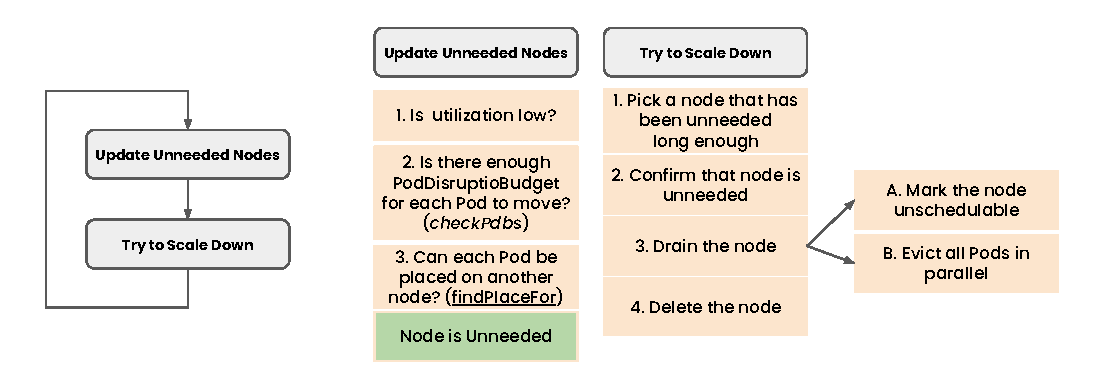
\includegraphics[width=1.1\textwidth]{resources/autoscaler-scale-down-process.pdf}
      }
      \caption{Cluster Autoscaler: Scale-down procedure}
      \label{figure:autoscaler-scale-down}
\end{figure}

We will use symbolic names to refer to various parameters of the Autoscaler in
our analysis, presented in Table \ref{table:symbolic-names-autoscaler}.
\begin{table}
      \begin{tabularx}{\linewidth}{|L|L|}
            \hline
            \textbf{Symbolic Name}        & \textbf{Description}                 \\ \hline
            scanInterval                  & How often cluster is reevaluated for
            scale up or down.
            \\
            \hline
            scaleDownDelayAfterAdd        & How long after scale up that scale
            down evaluation resumes. Defaults to 10 minutes. Configurable via
            the \co{--scale-down-delay-after-add} flag.                          \\
            \hline

            scaleDownDelayAfterDelete     & How long after node deletion that
            scale down evaluation resumes. Defaults to scanInterval.
            Configureable via the \co{--scale-down-delay-after-delete} flag.      \\
            \hline

            scaleDownDelayAfterFailure    & How long after scale down failure
            that scale down evaluation resumes. Defaults to 10 minutes.
            Configurable via the \co{--scale-down-delay-after-failure} flag.     \\
            \hline

            scaleDownUtilizationThreshold & Utilization threshold below which a
            node can be considered for scale down. Defaults to 0.5. Configurable
            via the \co{--scale-down-utilization-threshold} flag.                \\
            \hline

            scaleDownUnneededTime         & How long a ready node should be
            unneeded before it is eligible for scale down.  Defaults to 10
            minutes. Configurable via the \co{--scale-down-unneeded-time} flag.
            \\
            \hline

            scaleDownUnreadyTime          & How long an unready node should be
            unneeded before it is eligible for scale down.  Defaults to 20
            minutes. Configurable via the \co{--scale-down-unready-time} flag.
            \\
            \hline
      \end{tabularx}
      \caption{Symbolic names for various parameters of the Autoscaler used in our analysis}
      \label{table:symbolic-names-autoscaler}
\end{table}


\subsubsection{Update Unneeded Nodes Procedure}
The \textit{update unneeded nodes} procedure calculates which nodes of the
cluster have been unneeded and updates the Autoscaler's internal state with the
duration they have been unneeded. The Autoscaler considers a node
\textit{unneeded} if it meets all the following criteria:
\begin{itemize}
      \tightlist
      \item It is \textit{underutilized}, i.e., it has resource utilization
            below a specific threshold.
      \item The Pods that run on the node can be evicted (see section
            \ref{section:background-eviction}), i.e., their eviction is not
            blocked by any PodDisruptionBudgets.
      \item The Pods that run on the node can be moved to a different cluster
            node.
\end{itemize}
If a node does not meet the criteria, it is considered \textit{unremovable}.

To determine if an underutilized node is unneeded, the Autoscaler runs these
steps:
\begin{enumerate}
      \tightlist
      \item Calculate the Pods that must be moved if it removes the node.
      \item Check if any PodDisruptionBudgets block the eviction of any Pod. If
            so, the node is unremovable.
      \item Call \co{FindPlaceFor()} to find place for the Pods on a different
            node. \co{FindPlaceFor()} uses the
            \co{SchedulerBasedPredicateChecker} interface to determine if the
            Pod can be placed on any other node. It checks if the Pod can fit a
            node due to other scheduling constraints (CPU, memory), as well as
            if the Pod's volumes can be accessed from the node.
\end{enumerate}


The steps for  calculating the unneeded nodes are shown in
Algorithm~\ref{algo:update-unneeded}.

\subsubsection{Try to Scale Sown Procedure}

If a \textit{Ready} node remains unneeded for longer than
\co{scaleDownUnneededTime}, or an \textit{Unready} node remains unneeded for
longer than \co{scaleDownUnreadyTime} (see Table
\ref{table:symbolic-names-autoscaler} for the symbolic names) the Autoscaler
will consider the node as a candidate for deletion.

The Autoscaler makes a distinction between non-empty and empty nodes:
\begin{itemize}
      \tightlist
      \item \textit{Empty nodes}: nodes that run \textit{only} DaemonSet Pods.
            The Autoscaler removes them in bulk
      \item \textit{Non-empty nodes}: nodes that do not run only DaemonSet Pods.
            The Autoscaler removed them one by one to ensure that no Pods would
            be made unschedulable.
\end{itemize}

The algorithm for \co{TryToScaleDown()} is shown in
Algorithm~\ref{algorithm:try-scale-down}.

\paragraph*{Node removal} The node removal is executed as follows:
\begin{enumerate}
      \tightlist
      \item Add the \co{ToBeDeletedByClusterAutoscaler:NoSchedule} taint on the
            Node, essentially marking the node as unschedulable.
      \item Start draining the node by evicting in parallel all the Pods of the
            node. If any Pod can not be evicted due to a configured PDB, retry
            until the \co{MaxPodEvictionTimeout} exceeds.
      \item When all Pods are successfully evicted, ask the cloud provider to
            delete the node instance.
\end{enumerate}

The algorithm for the node removal is shown in
Algorithm~\ref{algorithm:node-delete}.


\clearpage
\begin{algorithm}[H]
    \caption{Cluster Autoscaler: Scale-down evaluation procedure}\label{alg:scale-down-evaluation}
    \SetKwIF{If}{ElseIf}{Else}{if~\endgraf}{\endgraf then}{else if}{else}{end if}%
    %\begin{minipage}{\textwidth}
    \begin{enumerate}[leftmargin=0cm]
        \tightlist
        \item Take a snapshot of the cluster Nodes, Pods, and PodDisruptionBudgets.
        \item \texttt{allNodes} \(\leftarrow\) List all the \co{Node} objects from the API Server.
        \item \texttt{scaleDownCandidates} \(\leftarrow\) Select nodes from
              \texttt{AllNodes} that belong to node groups that have not reached their
              minimum size.
        \item \texttt{podDestinations} \(\leftarrow\) \texttt{AllNodes};
              \texttt{podDestinations} represents the nodes that that may accept Pods in case a node is removed.
        \item Call \texttt{UpdateUnneededNodes()} with \texttt{podDestinations},
              and \texttt{scaleDownCandidates} as input, to calculate which nodes are
              unneeded an which ones are unremovable.
        \item \uIf{\begin{tabular}{@{\hspace*{1.0em}}l@{}}
                      the scale-down has been disabled for this loop                                           \\
                      % TODO: times in table
                      \textbf{OR} \co{scaleDownDelayAfterDelete} interval has not elapsed  \\
                      \textbf{OR} \co{scaleDownDelayAfterAdd} interval has not elapsed  \\
                      \textbf{OR} \co{scaleDownDelayAfterFailure} interval has not elapsed 
                  \end{tabular}}{
                  Don't scale-down the cluster. Autoscaler Status: \texttt{ScaleDownInCooldown}
              }
              \uElseIf{there is non empty node deletion in progress} {
                  Don't scale-down the cluster. Autoscaler Status: \texttt{ScaleDownInProgress}}
              \lElse{Try to scale down the cluster.}
    \end{enumerate}
    %\end{minipage}
\end{algorithm}


\begin{algorithm}[ht]
    \caption{Cluster Autoscaler: UpdateUnneededNodes() method}\label{algo:update-unneeded}
    \KwIn{\texttt{scaleDownCandidates}: a list of nodes that belong to
        node groups that have not reached their minimum size }
    \KwResult{Update the
        state of the Autoscaler with information about which nodes are unneeded}
    \begin{enumerate}[leftmargin=0.5cm]
        \tightlist
        \item For each node in \texttt{scaleDownCandidates}, call \texttt{checkNodeUtilization()}:
              \begin{enumerate}[]
                  \tightlist
                  \item \lIf{node has the ``ToBeDeletedByClusterAutoscaler'' taint}{ it is currently deleted, continue to next node}
                  \item \lIf{node has ``cluster-autoscaler.kubernetes.io/scale-down-disabled: true'' annotation}{continue to next node}
                  \item Calculate the utilization of the node.
                  \item \lIf{utilization is above threshold}{continue to next node}
                  \item Add the node \texttt{currentlyUnneededNodes}.
              \end{enumerate}
        \item \texttt{currentlyUnneededNonEmptyNodes} \lar From \texttt{currentlyUnneededNodes} select nodes that are not empty, i.e., they do not run only DaemonSet Pods.
        \item Call \texttt{findNodesToRemove(currentlyUnneededNonEmptyNodes)} to determine nodes that can be removed. For each node:
              \begin{enumerate}[]
                  \tightlist%        
                  \item Get the Pods that are running on the node and for each Pod:
                        \begin{enumerate}[leftmargin=0.5cm]
                            \tightlist
                            \item \lIf{the Pod has a Pod disruption budget that prevents its eviction}{the node is unremovable}
                            \item Call \texttt{findPlaceFor(pod)} to determine if it can be moved elsewhere.
                            \item \leIf{the Pod can not be moved elsewhere}{the
                                      node is unremovable}{the node can be removed, add it to
                                      \texttt{nodesToRemove}}
                        \end{enumerate}
              \end{enumerate}
        \item For each node in \texttt{nodesToRemove} update the state of the Autoscaler with the duration the node has been unneeded.
    \end{enumerate}
\end{algorithm}

\begin{algorithm}[ht]
\caption{Cluster Autoscaler: TryToScaleDown() method}\label{algorithm:try-scale-down}
    \KwIn{A list of unneeded nodes, as computed by UpdateUnneded() method}
    \KwResult{Scales-down the cluster}
\begin{enumerate}[leftmargin=0.5cm]
\item
  For each node in the unneeded nodes:

  \begin{enumerate}[leftmargin=0.5cm]
  \tightlist
  \item \lIf{If the node has the \texttt{cluster-autoscaler.kubernetes.io/scale-down-disabled}}{mark the node unremovable, reason \co{ScaleDownDisabledAnnotation}, go to next node.}
    \item
    \lIf{the node is \texttt{Ready}, and it has been underutilized for
    less than \texttt{ScaleDownUnneededTime}}{mark the node unremovable,
    reason \texttt{NotUnneededLongEnough}, continue to next node}
  \item
    \lIf{the node is \texttt{Unready}, and it has been underutilized for
    less than \texttt{ScaleDownUnreadyTime}}{mark the node unremovable,
    reason \texttt{NotUnreadyLongEnough}, continue to next node}
  \item
    Get the NodeGroup the node belongs to, get its \co{minSize} and current
    \co{size}, the number of node deletions in progress for the node group
    (\texttt{deletionsInProgress}).
  \item \lIf{\co{size} - \co{deletionsInProgress} $\leq$ \co{minSize}}{
    mark the node unremovable, reason \texttt{NodeGroupMinSizeReached},
    continue to next node}
  \end{enumerate}
  \item
  \co{candidates} \lar All the unneeded node that were not marked unremovable
  \item
    From \co{candidates}, try to scale-down as many as possible empty nodes.
  \item
    \texttt{nodesToRemove} \lar From the remaining candidates find nodes to
    remove (call \texttt{FindNodesToRemove()}).
  \item
    Pick a node from \texttt{nodesToRemove} and delete it
    (call \texttt{deleteNode()}) .
\end{enumerate}
\end{algorithm}
\begin{algorithm}[ht]
\caption{Cluster Autoscaler: deleteNode() method}\label{algorithm:node-delete}
    \KwIn{An unneeded Node of the Cluster to be deleted}
     \KwResult{Deletes the Node from the cluster and the Cloud Provider}
        \begin{enumerate}[leftmargin=0.5cm]
        \tightlist
        \item Add \co{ToBeDeletedByClusterAutoscaler:NoSchedule} taint on the
        Node to make the Node unschedulable.
        \item Drain the node; For each Pod (except for the DaemonSet Pods), in parallel:
            \begin{enumerate}
                \tightlist
                \item Send Eviction request
                \item \lWhile{the Eviction fails and for duration up to \co{MaxPodEvictionTimeout}}{retry the Eviction}

                Note: \co{MaxPodEvictionTimeout} is a hard-coded value equal to 2 minutes.
            \end{enumerate}
        \item \lIf{any of the Pods was not evicted successfully}{return error}
        \item \lIf{the node has any annotation with prefix
        \co{delay-deletion.cluster-autoscaler.kubernetes.io/}}{wait for up to
        \co{nodeDeletionDelayTimeout} for the annotation to be removed}
        \item Request from the Cloud Provider to delete the Node.
        \item \lIf{the Cloud Provider deletion fails}{return error}
        \end{enumerate}
\end{algorithm}


\clearpage
\subsection{Scale-Up}
\label{section:design-scale-up}
If the cluster has unschedulable Pods, the Autoscaler will try to help them by
adding new nodes to the cluster (\textit{scale-up}). A scale-up, essentially, is
the increase of the target size of one or more node groups. If multiple node
groups exist in the cluster, the cluster has to decide the following:
\begin{itemize}
      \tightlist
      \item Which node groups can help the unschedulable Pod run.
      \item How many nodes of the node group do the Pods need.
      \item If different node group scale-ups are feasible, which node group
            shall scale up.
\end{itemize}

As soon as the Autoscaler increases the target size of a node group, the cloud
provider will spin up new node instances, the new nodes will join the Kubernetes
cluster, and the scheduler will gradually scheduler the so far unschedulable
Pods to the new nodes.

The full algorithm for the \texttt{ScaleUp()} method is shown in
Algorithm~\ref{algorithm:scale-up}.

% TODO We show or is shown 
\paragraph*{Scale-up options}
To decide whether the scale-up of a node group would help the unschedulable Pod,
the Autoscaler runs the (roughly) following steps:
\begin{enumerate}
      \tightlist
      \item Take a snapshot of the cluster.
      \item Add a template node of the node group to the snapshot.
      \item Run a simulation, using the \co{SchedulerBasedPredicateChecker},
            whether the unschedulable Pod can be scheduled on the modified
            snapshot of the cluster.
      \item If the simulation determines that the Pod can be scheduled on the
            modified snapshot, use the \co{BinPackingNodeEstimator} to calculate
            how many nodes of that node group are needed.
\end{enumerate}

The option to scale up a specific node group with the number of needed nodes is
referred to as a ``\textit{scale-up option}''.

The complete algorithm to calculate a scale-up option is shown in Listing
\ref{algorithm:scaleup-options}.

\paragraph*{Scale-up strategy}

If multiple scale-up options, i.e., different node group scale-ups, can help the
unschedulable Pods, the Autoscaler decides which one is best using the
\co{Strategy} interface. There are various strategies, and the administrator can
configure the Autoscaler to use a desired one, e.g., the least cost option,
random strategy, etc.


\begin{algorithm}[ht]
    \caption{Cluster Autoscaler: ScaleUp() method}\label{alg:cap}
    \label{algorithm:scale-up} \KwIn{\co{pods}: the unschedulable Pods
        \\\co{snapshot}: the cluster snapshot } \KwResult{Adds extra nodes to
        accommodate the unschedulable Pods}
    \begin{enumerate}[leftmargin=0.5cm]
        \tightlist
        \item Build Pod equivalence groups - each Pod equivalence group consists
              of Pods that are managed by the same controller (same UUID) and have
              the same spec and labels.
        \item For each node group registered:
              \begin{enumerate}
                  \tightlist
                  \item Get its target size.
                  \item If the target size $\geq$ max size, go to the next node
                        group.
                  \item Create a template node for the node group.
                  \item Compute the expansion option for the node group, see
                        \co{ComputeExpansionsOption()}.
                  \item If any unschedulable Pod can be helped by adding a new
                        node of the node group, add the node group in the expansion
                        options list.
              \end{enumerate}
        \item If there are not any expansion options list, then do not trigger
              any scale-ups.
        \item Else, from the expansions options select one, according to the
              configured expansion strategy.
        \item Execute the selected scale up option: increase the target sizes of
              the corresponding node groups.
    \end{enumerate}
\end{algorithm}

\begin{algorithm}[ht]
    \caption{Cluster Autoscaler: ComputeExpansionsOption()
        algorithm}\label{algorithm:scaleup-options} \KwIn{\co{pods}: the unschedulable
        Pods \\\co{snapshot}: the cluster snapshot \\\co{template}: the template
        node of the node group} \KwResult{Computes if the scale-up of the node group
        would help any of the unschedulable Pods.}
    \begin{enumerate}[leftmargin=0.5cm]
        \tightlist
        \item
              For each Pod equivalence group:
              \begin{enumerate}
                  \tightlist
                  \item Get the sample Pod of the Pod equivalence group.
                  \item Add the template node in the cluster snapshot.
                  \item Call the Predicate Checker to check if any of the
                        unschedulable Pods can be scheduled in the new cluster snapshot.
                  \item If the sample Pod fits the new node in the cluster
                        simulation, append all the equivalent Pods in the list of Pods
                        that got helped (\co{options.Pods}).
              \end{enumerate}
        \item Call the bin-packing estimator to estimate how many nodes of
              the node group would be needed to help all the equivalent Pods.
        \item Return the \co{option}: a struct that indicates how many nodes of
              the node group are needed and which Pods would be helped.
    \end{enumerate}
\end{algorithm}



\clearpage
\subsection{Shortcomings \& Proposed Extensions}

In previous sections, we described the algorithms that govern the operations of
the Autoscaler; we will now identify their shortcomings.

\subsubsection{Scale-Down: Rok Volumes Can Be Migrated}
\label{section:design-autoscaler-unpinned}

When evaluating the scale-down of a node, the Autoscaler tries to find a place
for the Pods that run on the node in other cluster nodes. To do so, it calls the
\co{FindPlaceFor()} method, which in turn leverages the \co{PredicateChecker}
interface methods to determine if a Pod fits a node. The
\co{SchedulerBasedPredicateChecker} implementation of the interface runs the
VolumeBinding plugin's \co{Filter()} method to check if the volumes of the Pod
can be accessed from another node.


The PVs of the Rok storage class have node affinity that matches only with the
node where the volume was provisioned. Since the node affinity of the volumes
does not match any other in the cluster, the Autoscaler considers that the Pod
and its volume can not be moved on a different node, thus, marking the current
node as unremovable. The \co{SchedulerBasedPredicateChecker} does not know that
the Rok volumes have a mechanism to snapshot and recover them on a different
node [by unpinning them (snapshot + remove volume's node affinity, see section
            \ref{section:design-unpin}) and then pinning them (restoring the data) on
            another node ].

We propose the extension of the Autoscaler to simulate the Rok volumes as
unpinned (as if they do not have node affinity) when evaluating a scale-down
(and only then; in other cases, the volumes are retaining their node affinity).
With this extension, the Autoscaler will comprehend that the Rok volumes can
move anywhere in the cluster, and it can remove the node safely.

\subsubsection{Scale-Down: Coordinate With the Rok CSI Guard Mechanism}

As part of the Rok volume protection mechanism (see section
\ref{section:background-rok-csi-guard}), we deploy a \texttt{Deployment} object
for each node of the cluster, which creates a Pod per node (Rok CSI Guard)  with
strict node affinity that matches only the node it protects. The Autoscaler
tries \textit{to find place} to move this Pod. Since the Pod has strict node
affinity that matches only the current node, SchedulerBasedPredicateChecker
assumes that the Pod cannot be moved to a different node. Because of that, the
Autoscaler marks the node as unremovable. Of course, the Rok Operator will
remove the Pod after the Autoscaler removes the node, but the Autoscaler is
unaware of this fact.

Moreover,  the Autoscaler checks the PDB of the Guard Pod. The PDB of the Guard
Pod is configured to cause any evictions to fail. The Autoscaler notices that
and assumes that the Guard Pod will not be able to get safely evicted, thus,
marking the node unremovable. It is unaware that the Rok Operator will remove
them as soon as the scale-down starts and the Rok CSI  unpins all the local
volumes of the node.

We propose the extension of the Autoscaler so that it does not try to find a
place for the operator-managed ephemeral Guard Pods. Moreover, we extend the
Autoscaler to ignore the PDB of the Guard Pod. Still, the Autoscaler will be
aware that the Guard Pod exists, evicting it when it drains the node. This
eviction will fail as long as the PDB exists and the Autoscaler will retry,
delaying the deletion of the node.

To make things more obvious, here is the procedure that will take place with the
new design:


\begin{enumerate}
      \tightlist
      \item The Autoscaler evaluates a node for removal:
            \begin{enumerate}
                  \item It checks if the PDB allows the eviction of the Pods
                        running on the node, but it ignores the PDB of the Guard
                        Pod.
                  \item It tries to find a place for each Pod on a different
                        node, but it ignores the Guard Pod.
            \end{enumerate}
      \item The Autoscaler decides to remove the node.
      \item The Autoscaler adds the deletion taint on the node, effectively
            marking it as unschedulable for Pods.
      \item The Autoscaler sends eviction requests for each Pod to the API
            Server.
      \item The eviction of all the Pods --except for the Guard Pod-- succeeds.
      \item The Autoscaler keeps retrying to evict the Guard Pod, but the API
            Server responds that the eviction is not allowed due to the
            configured PDB.
      \item The Rok CSI Controller notices that the node is unschedulable and
            that no workload mounts the volumes, so it starts unpinning them.
      \item The Rok CSI Controller finishes the unpinning of the PVs.
      \item The Rok Operator removes the PodDisruptionBudget of the Guard Pod.
      \item The Autoscaler's request to evict the Guard Pod succeeds since the
            PDB was removed.
      \item The Autoscaler asks the cloud provider to delete the node.
      \item The Rok Operator removes the Rok CSI Guard \texttt{Deployment}
            object that corresponds to the removed node.
\end{enumerate}

Let us notice that the Autoscaler keeps retrying the eviction of the Guard Pod
for up to 2 minutes. That duration is a hard-coded timeout that might not be
enough in most cases. Taking a snapshot of the volume may last more than 2
minutes, depending on the size of the volume. It would be wise to use more sane
values and allow the user to cluster's admin to configure the value when
deploying the Autoscaler. To do so, we propose the extension of the Autoscaler
with a flag to configure the max pod eviction timeout.

\label{section:design-autoscaler-guards}


\subsubsection{Scale-Down: Consider Storage Capacity}

The Autoscaler shall check if the Rok volumes of a Pod can fit a node concerning
their requested storage capacity when evaluating a scale-down. As we have
explained, the Autoscaler used the \texttt{SchedulerBasedPredicateChecker}
interface in order to check if a Pod fits a node, which --among others-- calls
the VolumeBinding plugin's \co{Filter()} method.

We propose the extension of the SchedulerBasedPredicateChecker's VolumeBinding
plugin's \co{Filter} method: When evaluating if a Pod can be moved to a
different node, check if there is enough available storage on the node to move
the volumes.

Moreover, since the snapshotting and migration of a volume is a procedure that
costs in terms of time, the  Autoscaler shall not remove nodes with high storage
utilization, similarly to how it handles the CPU and memory resources. To
achieve this, we propose the extension of the Autoscaler with a new metric,
called the (Rok) ``\textit{storage utilization}'', defined as the ratio of the
used storage over the max storage capacity of the node. The Autoscaler will
compare this metric against a threshold configurable by the admin via a
corresponding flag; if the storage utilization exceeds the threshold, the node
will be considered unremovable.

\subsubsection{Scale-Down: Do Not Remove Unready Nodes}

A node that with status \co{Ready} can become \co{Unready} (or \co{NotReady}) if
a system problem on the node arises. Common reasons include lack of resources on
the node, a problem with the kubelet, an error related to kube-proxy, or a
networking problem in general.

The Autoscaler removes any unneeded Unready node after the
\texttt{scaleDownUnreadyTime} elapses. In the case of local volumes, we assume
that the node will always be in good condition, with all the systems up and
running and having network access, so Rok snapshots the local volumes to
Amazon's S3 remote storage. If that does not hold, removing a node will probably
cause any local data to be permanently lost.

The Autoscaler must not remove Unready nodes. The Unready nodes shall remain in
the cluster so that an administrator takes action to recover them from the
Unready state. We propose the extension of the Autoscaler with a flag to
explicitly disable the scale-down for nodes in \co{Unready} state and consider
them unremovable.

\subsubsection{Scale-Up: Consider Storage Capacity}
The Autoscaler does not know how much local storage is available when a new node
is spanned up and added to the cluster. The template node it creates from a live
node contains information only for the \textit{currently} free storage (of the
live node), reported on the capacity annotation by the storage driver (see the
proposed scheduler design, section \ref{section:capacity-annotation}). We need a
mechanism to know how much free storage a new node of a node group will have,
and the Autoscaler shall consider it in its simulations.

\paragraph*{Report max capacity}
Assuming that all the nodes in a node group have the same disk configuration and
max storage capacity, we can use the storage driver to report what the new
node's storage capacity would be on the \co{Node} objects. We propose the
extension of the Rok CSI Node component to report the max capacity of a node as
a label on the \co{Node} object. This label will be referred to as the
``\textit{max capacity label}'' \footnote{The \textit{Rok max capacity label}:
      rok.arrikto.com/max-instance-capacity}.

We use a label instead of an annotation because various cloud providers give the
cluster admins the option to pass labels to the node group node templates the
cloud provider plugin constructs. In case no live node for the node group
exists, the Autoscaler will construct the template from the cloud provider
plugin and have the configured admin labels on it.

At this point, let us distinguish the two reported quantities:
\begin{itemize}
      \tightlist
      \item \textit{capacity annotation}: the remaining free storage of a live
            node. The storage driver reports it, and the scheduler considers it
            when scheduling Pods.
      \item \textit{max capacity label}: the max storage capacity of the live
            node. i.e., the total storage capacity. That is a time constant
            value that depends on the node's disks.
\end{itemize}

For example, a node might have 200 Gi total storage (reported on the max
capacity label), and only 100 Gi out of them are free (reported on the capacity
annotation).

\paragraph*{Pass the max capacity information to the template}

For the Autoscaler to simulate the scheduling with capacity considerations, we
will import in the SchedulerBasedPredicateChecker the extended VolumeBinding
(see section \ref*{section:volume-plugin-extensions}).

The extended VolumeBinding plugin will look for the capacity of a template node
on the capacity annotation and not on the label. Since the template will get the
annotation from a live node, it will represent the currently free storage on the
live node instead of the max storage capacity. We need to sanitize the value and
set it to the actual max capacity. To do so, we propose the extension of the
sanitization mechanism of the Autoscaler to copy the max capacity label's value
to the capacity annotation. In this way, the template node's capacity annotation
will indicate the max capacity (total) storage of the new node of the node
group.

The sanitization mechanism shall set the capacity annotation to an infinitely
large value if the max capacity label does not exist. This design choice offers
the following advantages:
\begin{enumerate}
      \item The Autoscaler treats the node as if it had infinite storage
            capacity and will add a live node of the node group (scale-up). If
            the decision was wrong (\textit{false scale-up}), i.e., the added
            node does not have enough storage capacity for the Pod that
            triggered the scale-up, the scheduler of the cluster will not assign
            the Pod to the newly added node. As a result, the node will remain
            unneeded, and the Autoscaler will remove it after some time. The
            system will gradually fix the wrong decision.
      \item The wrong node addition allows the Autoscaler to learn the actual
            max capacity of the node. The Rok CSI driver gets the chance to run
            on the node, and the Autoscaler generates a template node from the
            live node, which contains accurate information for the max available
            capacity reported by the Rok CSI driver.
\end{enumerate}


\paragraph*{Wait for Rok CSI to run}

If a Pod triggers a scale-up because of the storage it requests, it may take a
reasonable time from the node addition till the Rok CSI driver starts running on
the node. As long as the Rok CSI is not running on the node, the corresponding
capacity annotation is not set on the \co{Node} object. The scheduler does not
schedule the Pod on the node since the absence of the annotation indicates the
storage is unavailable (see Section ~\ref{section:design-volume-binding}). The
Autoscaler runsthe scheduling simulation and decides that the Pod does not fit
the newly added node (since the live node has no capacity annotation), so it
triggers a new scale-up.

To resolve this issue, the Autoscaler must wait for the Rok CSI driver to run on
the newly added node. As long as the driver does not run on a new node (i.e.,
the node does not have the capacity label set), the Autoscaler shall replace the
node with an \textit{Unready} copy.

The Autoscaler treats Unready nodes as upcoming nodes (for a duration of up to
15 minutes): it replaces them with template nodes of the node group they belong
to in its simulations. The template node will have the capacity annotation set
as if the Rok CSI was running. The Autoscaler's simulation will assume that Pod
will be scheduled on the node when the Rok CSI is ready and running and will not
trigger any further scale-up.

We mentioned that the Autoscaler treats Unready node as upcoming for up to 15
minutes. That needs a bit of explanation. The Autoscaler gives the nodes a
reasonable amount to become fully Ready; after this duration, it will stop
replacing the Unready nodes with their template and will consider them
unschedulable in the simulation. If any Pods that relied on the node becoming
ready (in order to run there) still exist, they will now trigger another
scale-up. Of course, in the case of Rok, 15 minutes are more than enough for the
Rok CSI driver to become ready and start running.

\section{The Container Storage Interface}
\label{section:background-csi}

The \textit{Container Storage Interface} (CSI) is a standard for exposing
arbitrary block and file storage systems to containerized workloads on container
orchestration systems (COs), such as Kubernetes. Using CSI, third-party storage
providers can write and deploy plugins exposing new storage systems in
Kubernetes without ever having to touch the core Kubernetes code.

\subsection{CSI Driver Architecture}
\label{section:backgroud-csi-plugins-architecture}

Kubernetes interacts with a CSI driver plugin through \textit{Remote Procedure
      Calls} (RPCs). Each CSI driver consists of the following plugins:

\begin{itemize}
      \item
            \textbf{Node Plugin}: A gRPC endpoint serving CSI RPCs that must run
            on the node where the provisioned volume will be published. It
            consists of the CSI driver that implements the CSI \co{Node} service
            and one or more sidecar containers. The kubelet of every node is
            responsible for issuing the CSI Node service calls. The kubelet
            issues the calls to the Node service of the driver through a UNIX
            domain socket on the host shared via a \co{HostPath} volume. The
            node plugin has direct access to the host for making block devices
            and filesystem mounts available to the kubelet.
      \item
            \textbf{Controller Plugin}: A gRPC endpoint serving CSI RPCs that
            may run on any node of the cluster. It consists of the CSI driver
            that implements the CSI \co{Controller} service and one or more
            sidecar containers. These controller sidecar containers typically
            interact with Kubernetes objects and make calls to the driver's CSI
            Controller service by sharing a UNIX domain socket through an
            \co{emptyDir} volume between the sidecars and CSI driver. It
            generally does not need direct access to the host.
\end{itemize}

%TODO: Scheme drivers

\paragraph*{The Google Remote Procedure Call}

We mentioned earlier that a container orchestrator  interacts with the driver
through RPCs. The most widely used RPCs are \textit{Google Remote Procedure
      Calls} (gRPC). gRPC is an open-source, high-performance Remote Procedure Call
(RPC) framework that can run in any environment. It uses HTTP/2 for transport,
Protocol Buffers as the interface description language, and provides
authentication, bidirectional streaming and flow control features, blocking or
non-blocking bindings, and cancellation and timeouts. It generates
cross-platform client and server bindings for many languages. gRPC clients and
servers can run and talk to each other in various environments and can be
written in any of gRPC’s supported languages.

\begin{figure}[ht]
      \centering
      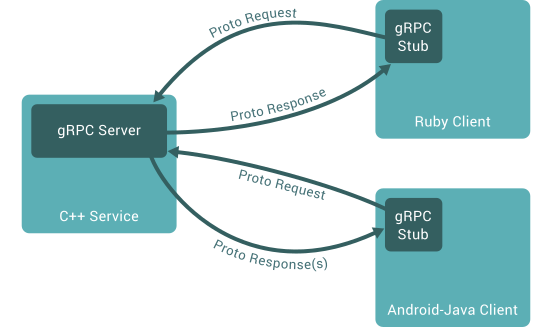
\includegraphics[width=0.6\textwidth]{resources/grpc.png}
      \caption{The architecture of gRPC}
\end{figure}


\subsection{The CSI Remote Procedure Calls}

\begin{figure}[ht]
      \centering
      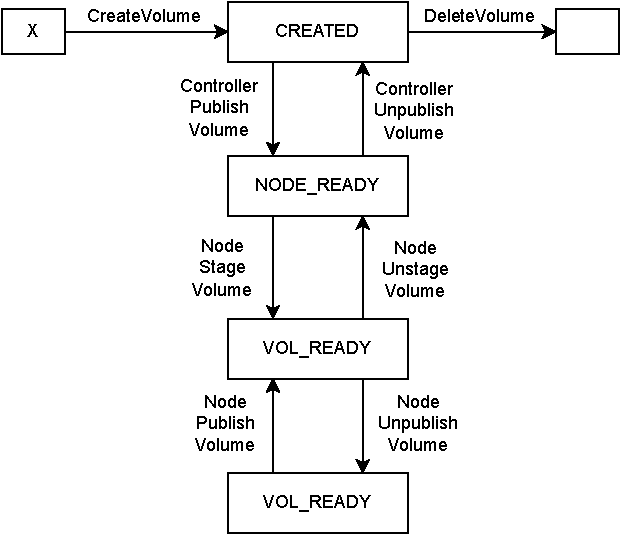
\includegraphics[width=0.7\textwidth]{resources/csi-states.pdf}
      \caption{The lifecycle of a dynamically provisioned volume, from creation
            to destruction.}
      \label{figure:csi-calls}
\end{figure}

The Container Storage Interface defines the RPCs a container orchestrator uses
in order to interact with the storage driver. Each of the RPCs is an idempotent
operation. The order the calls can be issued is show in Figure
\ref{figure:csi-calls}. The list of available RPCs is the following:

\begin{itemize}

      \item{\co{CreateVolume}}: The external provisioner issues this RPC to the
            CSI Controller service, asking it to provision a new volume on
            behalf of a user. If the plugin is unable to complete the
            \co{CreateVolume} call successfully, it must return a non-OK gRPC
            code in the gRPC status.

            Of particular interest in the context of the thesis is the
            \co{RESOURCE\_EXHAUSTED} code; If the controller plugin responds
            with this code, it indicates that it cannot provision the requested
            volume with the specified topology constraints, possibly due to
            insufficient storage capacity.

      \item{\co{ControllerPublishVolume}}: The external attacher issues
            this RPC to the CSI Controller service when Kubernetes wants to
            place a workload that uses the (already provisioned) volume onto a
            node. The plugin should perform the necessary work to make the
            volume available on the given node.

      \item{\co{NodeStageVolume}}:  The kubelet issues this RPC to the  CSI Node
            service when the volume is to be used by the first Pod on the node.
            It should be issued only after \co{NodePublishVolume} has succeeded.
            It is essentially used to format the volume and mount it on a
            staging directory on the node.

      \item{\co{NodePublishVolume}}: The  kubelet issues this RPC to the  CSI
            Node service when a Pod starts to run on a node. It essentially
            mounts the volume to the directory of the Pod.

      \item{\co{NodeUnpublishVolume}}: The kubelet issue this RPC to the CSI
            Node service to undo the work done by the corresponding
            \co{NodePublishVolume}. It essentially unmounts the volume from the
            directory of the Pod.

      \item{\co{NodeUnstageVolume}}: The kubelet issues the RPC to the CSI Node
            service to undo the work by the corresponding \co{NodeStageVolume}.
            It essentially unmounts the volume from the staging directory of the
            node.

      \item{\co{ControllerUnpublishVolume}}: The external attacher issues this
            RPC to the CSI Controller service to perform the work necessary for
            making the volume ready to be consumed by a different node. It
            essentially undoes any work done by the
            \co{ControllerPublishVolume}.

      \item{\co{DeleteVolume}}: The external provisioner issues this RPC to the
            CSI Controller service to deprovision a volume. It is the reverse
            operation of the \co{CreateVolume}.

\end{itemize}


\subsection{Kubernetes CSI Sidecars}
The Kubernetes CSI sidecars containers are a set of standard containers that aim
to simplify the development and deployment of CSI drivers on Kubernetes. These
containers contain common logic to watch the Kubernetes API, trigger appropriate
operations against the \textit{CSI driver} container, and update the Kubernetes
API as appropriate. The containers are intended to be bundled with third-party
CSI driver containers and deployed together as Pods.



\subsubsection{CSI External Provisioner}
\label{csi-external-provisioner}
\label{section:provisioner}

The CSI external provisioner is a sidecar container that watches the Kubernetes
API server for \texttt{PersistentVolumeClaim} objects. If a PVC requests for
dynamic provisioning of a volume and has the selected node annotation
\footnote{Selected node annotation: \co{volume.kubernetes.io/selected-node:
            <node-name>}}, the external provisioner issues a \co{CreateVolume} RPC against
the CSI Controller service to provision a new volume accessible from the
selected node. Suppose the Controller service responds with a
\co{ResourceExhausted} status code. In that case, the external provisioner will
remove the selected node annotation from the PVC, to signal back to the
scheduler that the provisioning of the volume has failed, and it shall retry the
scheduling. Once the external provisioner successfully provisions the volume, it
creates a Kubernetes \texttt{PersistentVolume} object to represent the volume
and binds it to the PVC.

The deletion of a \texttt{PersistentVolumeClaim} object bound to a
\texttt{PersistentVolume} corresponding to this driver with a \texttt{delete}
reclaim policy causes the external provisioner to trigger a
\texttt{DeleteVolume} operation against the CSI Controller service to delete the
volume. Once the volume is successfully deleted, the sidecar container deletes
the \texttt{PersistentVolume} object representing the volume.

\subsubsection{CSI External Attacher}

The CSI external attacher is a sidecar container that watches the Kubernetes API
server for \texttt{VolumeAttachment} objects and triggers
\co{ControllerPublishVolume} and \co{ControllerUnpublishVolume} operations
against a CSI endpoint.


\subsubsection{CSI Node Driver Registrar}

The CSI node driver registrar is a sidecar container that fetches driver
information  by issuing a \texttt{NodeGetInfo}) to the CSI Node service and
registers the driver with the kubelet on that node.  The registration is
necessary because the kubelet is responsible for issuing CSI \co{NodeGetInfo},
\co{NodeStageVolume}, \co{NodePublishVolume} calls. By registering the CSI
driver, the kubelet learns which Unix domain socket to issue the CSI calls on.
\subsection{Kubernetes CSI: An End-to-End Story}

In this section, we aim to combine all the information by describing an
end-to-end story for the CSI.  We present the timeline of actions that take
place under the hood in order to provision a  volume dynamically.

The timeline of actions is the following:

\begin{enumerate}
	\tightlist
	\item The cluster administrator creates a StorageClass (in our case, the
	      \co{Rok} storage class) that specifies the CSI plug-in name
	      (\co{provisioner:rok.arrikto.com}):
	      \lstinputlisting[language=yaml]{code/rok-sc.yaml}

	\item A user creates a PersistentVolumeClaim that requests a volume of at
	      least 10 Gi with access mode \co{ReadWriteOnce} from the \co{Rok}
	      storage class.

	      \lstinputlisting[language=yaml]{code/pvc-rok.yaml}

	      Since the \co{Rok} StorageClass has \co{volumeBindingMode:
		      WaitForFirstConsumer}, the volume for the PVC will not be
	      provisioned as long as a Pod requesting the PVC is not scheduled
	      on a node. he PVC to be provisioned.
	\item  A user creates a Pod that uses the PVC:
	      \lstinputlisting[language=yaml]{code/pod-pvc-rok.yaml}
	\item The VolumeBinding plugin of the scheduler does not find any PV to
	      match the PVC. It signals the driver to provision the volume
	      dynamically: it annotates the PVC with the selected node annotation..
	\item The external provisioner sidecar that runs along with the Rok CSI
	      driver sees the annotation on the PVC and issues a \co{CreateVolume}
	      call against the Rok CSI Controller service to provision the volume.
	\item The Rok CSI controller provisions the volume and returns a successful
	      response to the external provisioner.
	\item The external provisioner creates a \co{PersistentVolume} object on the API
	      Server and binds it (the PV) to the  PVC.
	\item The PersistentVolume controller completes the bidirectional binding of
	      the PV and the PVC (by binding the PVC to the PV).
\end{enumerate}
\section{Logical Volume Management}
\label{section:background-lvm}

Logical Volume Management enables combining multiple individual hard drives and
disk partitions into a single volume group (VG). That volume group can then be
subdivided into logical volumes (LV) or used as a single large volume. Regular
file systems, such as EXT3 or EXT4, can then be created on a logical volume.


Logical volume manager (LVM) introduces an extra layer between the physical
disks and the file system, allowing file systems to:
\begin{itemize}
      \tightlist
      \item
            Be resized and moved with ease and online without requiring a
            system-wide outage.
      \item
            Use discontinuous space on disk.
      \item
            Have meaningful names to volumes, rather than the usual cryptic
            device names.
      \item
            Span multiple physical disks.
\end{itemize}

\begin{figure}[ht]
      \centering
      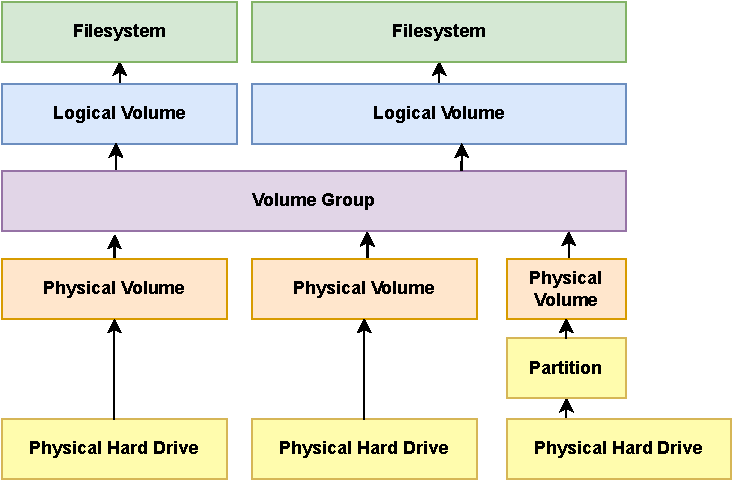
\includegraphics[width=0.8\textwidth]{resources/lvm.pdf}
      \caption{The Logical Volume Management layers}
\end{figure}

The Logical Volume Management consists of the following conceptual layers:
\begin{itemize}
      \item
            \textbf{Physical Volume}: Each Physical Volume can be a disk
            partition, whole disk, meta-device, or a loopback file.
      \item
            \textbf{Volume Group} (VG): A Volume Group gathers a collection of
            Logical Volumes and Physical Volumes into one administrative unit. A
            volume group is divided into fixed-size physical extents. VGs are
            made up of Physical Volumes, which, in turn, are made up of
            physical extents (PEs).

      \item
            \textbf{Logical Volume} (LV): A Logical Volume is the conceptual
            equivalent of a disk partition in a non-LVM system. Logical volumes
            are block devices that are created from the physical extents present
            in the same volume group.
\end{itemize}

\section{Rok's Local Volume Mechanism}

Local data on a node need a mechanism to be backed up if the node gets removed
from the cluster; otherwise, the data will be permanently lost, and the user
will not be able to recover them.

Rok provides a mechanism that enables the functionality of moving volumes around
the nodes of a cluster. It leverages an external storage system, such as
Amazon's S3, where it snapshots the local volumes and can restore them on a
different node. Rok refers to moving a local volume to Amazon S3 as
\textit{``Unpinning''} and restoring the volume to a different node as
\textit{``Pinning''}. We describe this mechanism in greater depth in the
following section.

\subsection{Rok Volume Pinning and Unpinning}

\label{section:rok-volume-pinning}

When a local volume is provisioned on a node, the corresponding
\co{PersistentVolume} object on the API Server that represents the volume has
node affinity on it (see section \ref{section:background-pv-node-affinity}). In
the case of local storage, the Rok CSI driver sets the node affinity of the PV
to match only with the node where the local volume is provisioned.


Rok introduces the following terms:
\begin{itemize}
	\tightlist

	\item \textit{Pinned PV}: A PV representing a node's local volume. This PV
	      has node affinity to indicate that it is accessible only from that
	      particular node.
	\item \textit{Unpinned PV}: A PV representing a local volume migrated to S3.
	      The PV has an empty node affinity to indicate that it is accessible
	      from every cluster node.
\end{itemize}

A pinned PV can become unpinned with the process of ``\textit{unpinning}''. An
unpinned PV can become pinned with the process of ``\textit{pinning}''. The
process can be repeated multiple times, essentially allowing the volume to move
around the cluster nodes as many times as needed.

\label{section:design-unpin}
The Rok CSI Controller implements the following mechanism for the unpinning of a
PV:
\begin{enumerate}
	\tightlist
	\item Watches for nodes that are marked unschedulable.
	\item Finds volumes on the unschedulable node that are not currently used by
	      any Pods.
	\item Starts the unpinning process of the unused PV: it takes snapshots of
	      the volume on Amazon S3.
	\item Removes the node affinity from the PV. Note that the \co{nodeAffinity}
	      field of a PV is immutable, i.e., it is not allowed to change. To
	      overcome this restriction, Rok deletes the PV and instantaneously
	      recreates it.
\end{enumerate}

Rok implements the following mechanism for the pinning of a PV:
\begin{enumerate}
	\tightlist
	\item The Scheduler schedules the Pod that references the unpinned PV
	      (through a PVC).
	\item The Kubernetes \co{attachDetach} controller creates a
	      \co{VolumeAttachment} object to signal the external attacher to attach
	      the volume on the node.
	\item The external attacher sees the VolumeAttachment and issues a
	      \co{ControllerPublishVolume} call to the Rok CSI controller.
	\item The Rok CSI controller creates a logical volume on the Rok VG and
	      restores the data of the PV from the Amazon S3 to the logical volume.
	\item The Rok CSI controller sets the appropriate node affinity on the PV to
	      indicate its only accessible from the node the volume was restored to.
\end{enumerate}


\subsection{Rok's Local Volume Protection Mechanism}
\label{section:background-rok-csi-guard}

The Kubernetes maintenance and upgrade tools rely on the \co{drain} operation
(see \ref{section:cordon-drain}). Essentially, before taking any actions to
remove or upgrade a node in the cluster, the tools drain the node (\co{kubectl
	drain}) in order to mark the node unschedulable and safely evict all the Pods.
The Cluster Autoscaler also uses the drain operation before removing a node.

Rok deploys a mechanism to facilitate the upgrades of a cluster and ensure that
the nodes are not removed before Rok snapshots all their local volumes.

The mechanism leverages Pods with properly configured PodDisruptionBudgets to
block their eviction. It relies on the fact that the drain operation fails as
long as the eviction of a Pod fails. The mechanism works as follows:

\begin{enumerate}
	\tightlist
	\item The Rok Operator creates a \co{Deployment} resource \textit{for each
		      node} in the cluster. The Deployment of each node creates
	      \textit{exactly} one replica Pod with node affinity that matches
	      only the specific node. Rok names these Pods  ``\textit{CSI Guard
		      Pod}'', since they protect the node's local volumes.
	\item The Rok Operator creates a \co{PodDisruptionBudget} object for each
	      Rok CSI Guard Deployment. The PodDisruptionBudget demands at any time
	      to exist at least one Rok CSI Guard Pod of the Deployment. This
	      configuration causes any evictions of the Rok CSI Guard Pod to fail.
	\item The drain operation marks the node unschedulable and starts evicting
	      the Pods on the node. The eviction of the CSI Guard fails because of
	      the configured PodDisruptionBudget.
	\item The Rok Operator checks if the Rok CSI has unpinned all the volumes of
	      the unschedulable node; if this condition holds, it removes the
	      PodDisruptionBudget that corresponds to the CSI Guard of the node.
	\item Since the PodDisruptionBudget does not exist anymore, the eviction of
	      the  Rok CSI Guard Pod finally succeeds, and the drain operation
	      completes.
\end{enumerate}

The mechanism is illustrated in Figure ~\ref{figure:rok-csi-guards}.

\clearpage
\vspace*{2cm}
\begin{figure}[H]
	\centering
	\makebox[\textwidth][c]{
		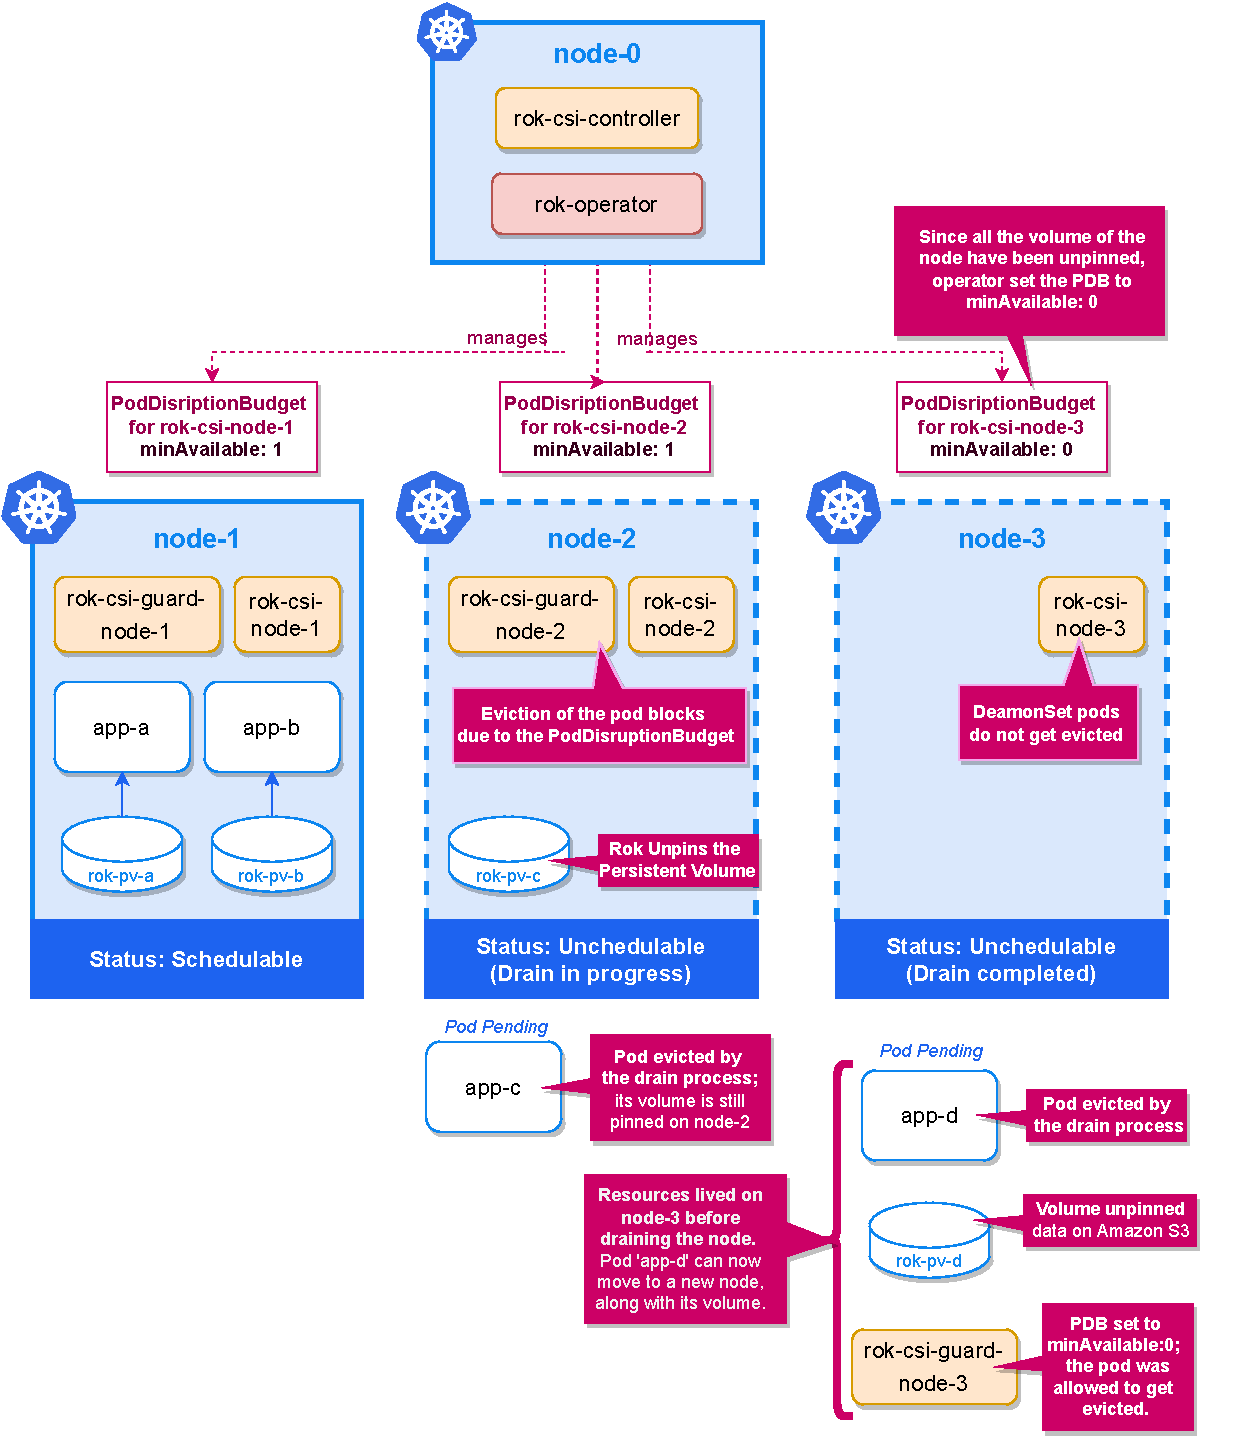
\includegraphics[width=1.2\textwidth]{resources/drain-cluster.pdf}
	}
	\caption{Protecting Local Data with Rok CSI Guard Pods}
	\label{figure:rok-csi-guards}
\end{figure}
\clearpage
\chapter{Design} \label{chapter:design}

In this chapter, we describe the design and algorithms that discipline the
operation of the Cluster Autoscaler and the Scheduler; we point out their
shortcomings concerning local data storage and propose design enhancements to
enable seamless scheduling and autoscaling with local persistent volumes.

\section{Design Rationale \& Goals}

As explained in section \ref{section:intro_problem_statement}, our goal is to
extend the Scheduler and the Cluster Autoscaler so that they operate seamlessly
with workloads that use volumes backed by local storage. More specifically, we
aim to:

\begin{itemize}
      \tightlist
      \item Extend the Scheduler to consider the storage capacity of the nodes
            when scheduling Pods.
      \item Extend the Autoscaler to scale-down nodes where local volumes live,
            ensuring that Rok's mechanism snapshots the data before removing the
            node from the cluster.
      \item Extend the Autoscaler to check if the Pod's volumes can be placed on
            any other node (with regards to storage capacity) when evaluating (for
            a possible scale-down) if a Pod can be moved elsewhere.
      \item Extend the Autoscaler to consider the storage capacity of nodes, and,
            when scaling up, add a node with enough storage capacity.
      \item Extend the Autoscaler to not remove unready nodes in case local
            volumes live on these nodes.
\end{itemize}

\section{Rok's Local Volume Mechanism}

Local data on a node need a mechanism to be backed up if the node gets removed
from the cluster; otherwise, the data will be permanently lost, and the user
will not be able to recover them.

Rok provides a mechanism that enables the functionality of moving volumes around
the nodes of a cluster. It leverages an external storage system, such as
Amazon's S3, where it snapshots the local volumes and can restore them on a
different node. Rok refers to moving a local volume to Amazon S3 as
\textit{``Unpinning''} and restoring the volume to a different node as
\textit{``Pinning''}. We describe this mechanism in greater depth in the
following section.

\subsection{Rok Volume Pinning and Unpinning}

\label{section:rok-volume-pinning}

When a local volume is provisioned on a node, the corresponding
\co{PersistentVolume} object on the API Server that represents the volume has
node affinity on it (see section \ref{section:background-pv-node-affinity}). In
the case of local storage, the Rok CSI driver sets the node affinity of the PV
to match only with the node where the local volume is provisioned.


Rok introduces the following terms:
\begin{itemize}
	\tightlist

	\item \textit{Pinned PV}: A PV representing a node's local volume. This PV
	      has node affinity to indicate that it is accessible only from that
	      particular node.
	\item \textit{Unpinned PV}: A PV representing a local volume migrated to S3.
	      The PV has an empty node affinity to indicate that it is accessible
	      from every cluster node.
\end{itemize}

A pinned PV can become unpinned with the process of ``\textit{unpinning}''. An
unpinned PV can become pinned with the process of ``\textit{pinning}''. The
process can be repeated multiple times, essentially allowing the volume to move
around the cluster nodes as many times as needed.

\label{section:design-unpin}
The Rok CSI Controller implements the following mechanism for the unpinning of a
PV:
\begin{enumerate}
	\tightlist
	\item Watches for nodes that are marked unschedulable.
	\item Finds volumes on the unschedulable node that are not currently used by
	      any Pods.
	\item Starts the unpinning process of the unused PV: it takes snapshots of
	      the volume on Amazon S3.
	\item Removes the node affinity from the PV. Note that the \co{nodeAffinity}
	      field of a PV is immutable, i.e., it is not allowed to change. To
	      overcome this restriction, Rok deletes the PV and instantaneously
	      recreates it.
\end{enumerate}

Rok implements the following mechanism for the pinning of a PV:
\begin{enumerate}
	\tightlist
	\item The Scheduler schedules the Pod that references the unpinned PV
	      (through a PVC).
	\item The Kubernetes \co{attachDetach} controller creates a
	      \co{VolumeAttachment} object to signal the external attacher to attach
	      the volume on the node.
	\item The external attacher sees the VolumeAttachment and issues a
	      \co{ControllerPublishVolume} call to the Rok CSI controller.
	\item The Rok CSI controller creates a logical volume on the Rok VG and
	      restores the data of the PV from the Amazon S3 to the logical volume.
	\item The Rok CSI controller sets the appropriate node affinity on the PV to
	      indicate its only accessible from the node the volume was restored to.
\end{enumerate}


\subsection{Rok's Local Volume Protection Mechanism}
\label{section:background-rok-csi-guard}

The Kubernetes maintenance and upgrade tools rely on the \co{drain} operation
(see \ref{section:cordon-drain}). Essentially, before taking any actions to
remove or upgrade a node in the cluster, the tools drain the node (\co{kubectl
	drain}) in order to mark the node unschedulable and safely evict all the Pods.
The Cluster Autoscaler also uses the drain operation before removing a node.

Rok deploys a mechanism to facilitate the upgrades of a cluster and ensure that
the nodes are not removed before Rok snapshots all their local volumes.

The mechanism leverages Pods with properly configured PodDisruptionBudgets to
block their eviction. It relies on the fact that the drain operation fails as
long as the eviction of a Pod fails. The mechanism works as follows:

\begin{enumerate}
	\tightlist
	\item The Rok Operator creates a \co{Deployment} resource \textit{for each
		      node} in the cluster. The Deployment of each node creates
	      \textit{exactly} one replica Pod with node affinity that matches
	      only the specific node. Rok names these Pods  ``\textit{CSI Guard
		      Pod}'', since they protect the node's local volumes.
	\item The Rok Operator creates a \co{PodDisruptionBudget} object for each
	      Rok CSI Guard Deployment. The PodDisruptionBudget demands at any time
	      to exist at least one Rok CSI Guard Pod of the Deployment. This
	      configuration causes any evictions of the Rok CSI Guard Pod to fail.
	\item The drain operation marks the node unschedulable and starts evicting
	      the Pods on the node. The eviction of the CSI Guard fails because of
	      the configured PodDisruptionBudget.
	\item The Rok Operator checks if the Rok CSI has unpinned all the volumes of
	      the unschedulable node; if this condition holds, it removes the
	      PodDisruptionBudget that corresponds to the CSI Guard of the node.
	\item Since the PodDisruptionBudget does not exist anymore, the eviction of
	      the  Rok CSI Guard Pod finally succeeds, and the drain operation
	      completes.
\end{enumerate}

The mechanism is illustrated in Figure ~\ref{figure:rok-csi-guards}.

\clearpage
\vspace*{2cm}
\begin{figure}[H]
	\centering
	\makebox[\textwidth][c]{
		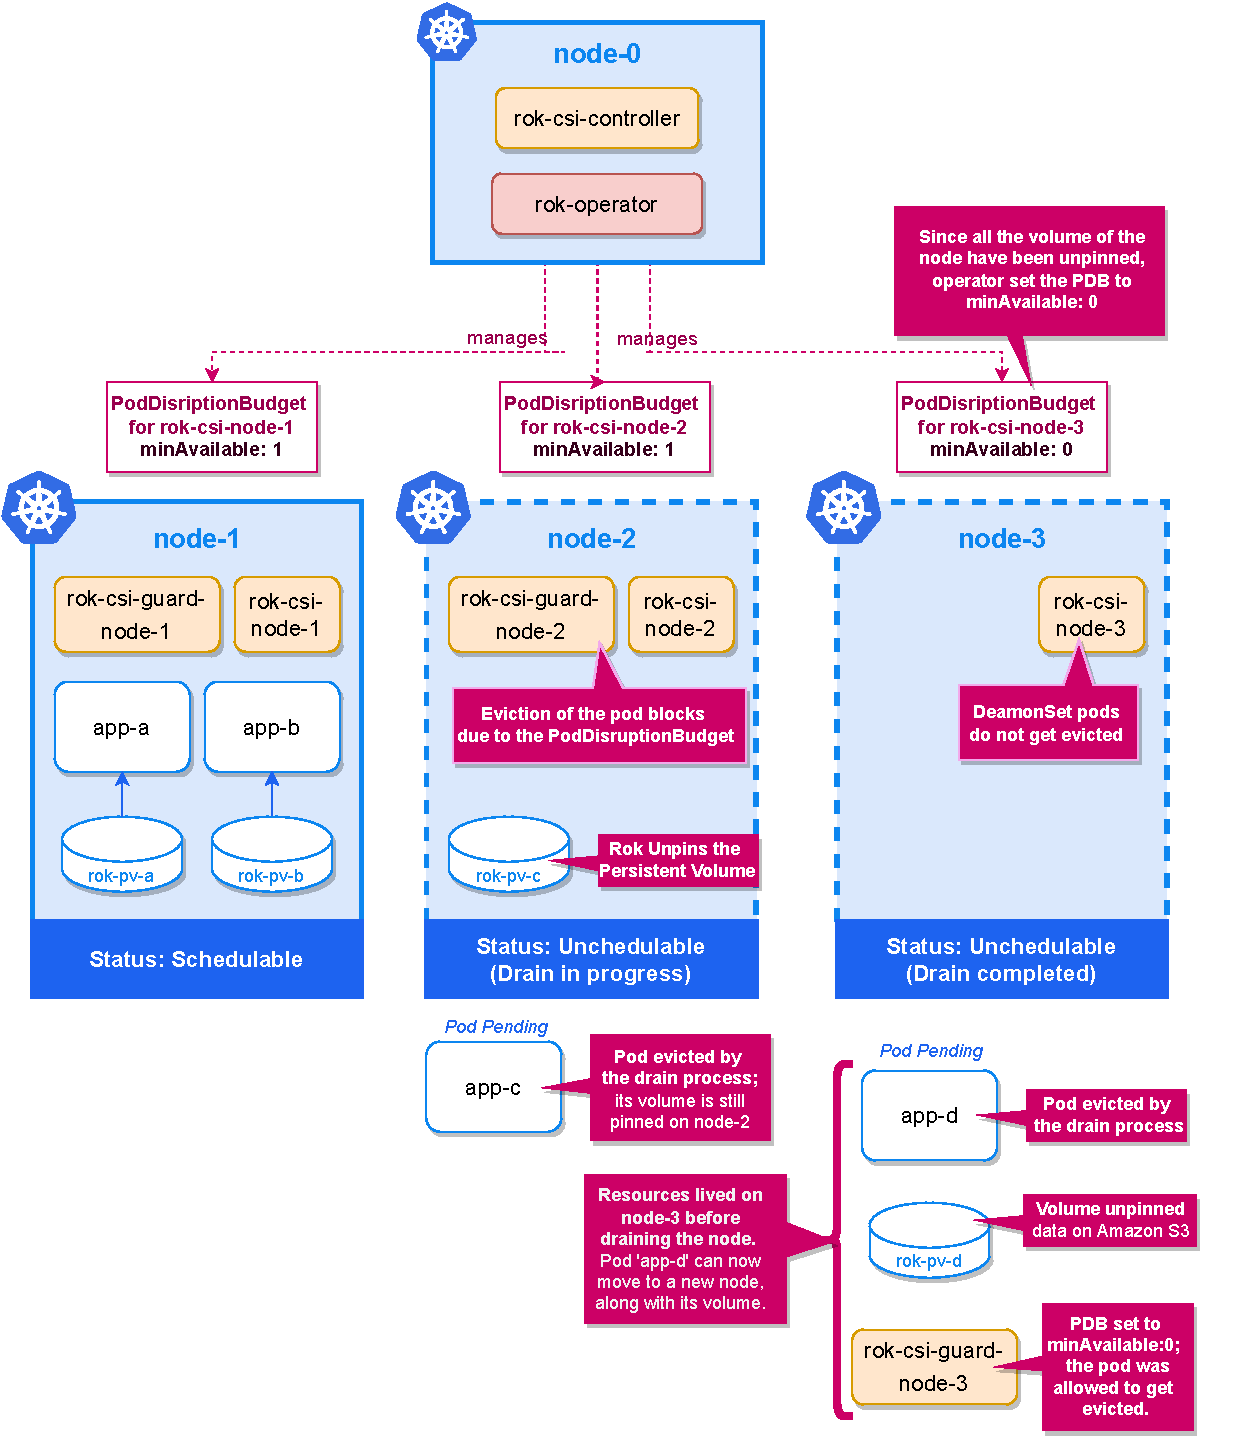
\includegraphics[width=1.2\textwidth]{resources/drain-cluster.pdf}
	}
	\caption{Protecting Local Data with Rok CSI Guard Pods}
	\label{figure:rok-csi-guards}
\end{figure}
\clearpage
\section{Kubernetes Scheduler}
\RestyleAlgo{ruled}

Σε αυτήν την ενότητα, θα παρουσιάσουμε συνοπτικά τη τρέχουσα σχεδίαση του
Kubernetes Scheduler, θα επισημάνουμε τις ελλείψεις που υπάρχουν και θα
προτείνουμε βελτιώσεις που επιλύουν τους τρέχοντες περιορισμούς.

\subsection{To Πρόσθετο VolumeBinding}

Για λόγους συντομίας, στο ελληνικό τμήμα της διπλωματικής παρουσιάζουμε μόνο τη
σχεδίαση της \co{Filter} και της \co{PreBind}  φάσης του προσθέτου, καθώς
σχετίζεται άμεσα με τις προτεινόμενες επεκτάσεις. Για την αναλυτική παρουσίαση
των υπολοίπων φάσεων του προσθέτου, μπορείτε να ανατρέξετε στο αντίστοιχο
αγγλικό κεφάλαιο, στην ενότητα \ref{section:design-volume-binding}.

\subsection*{PreFilter Φάση}

\co{Filter}: αξιολογεί αν ένα Pod μπορεί να τοποθετηθεί σε έναν κόμβο, βάσει των
τόμων που ζητά, τόσο για τα δεσμευμένα όσο και για τα μη δεσμευμένα PVC:
\begin{itemize}
      \tightlist
      \item Για τα \textit{δεσμευμένα PVC}, ελέγχει ότι το PV του κάθε PVC είναι
            προσβάσιμο (βάσει τoy node affinity που φέρει) από τον εξεταζόμενο
            κόμβο.
      \item Για τα \textit{μη δεσμευμένα PVC}, προσπαθεί να βρει διαθέσιμα PVs
            που μπορούν να ικανοποιήσουν τις απαιτήσεις του PVC και που είναι
            προσβάσιμα (βάσει του node affinity τους) από τον εξεταζόμενο κόμβο.
            Τα PVCs για τα οποία δεν κατάφερε να βρει κατάλληλα PVs, θα τα
            αποκαλούμε εφεξής ``\textit{PVCs to provision}''.
      \item Για κάθε \textit{PVC to provision}, ελέγχει αν η \co{StorageClass}
            του PVC υποστηρίζει τη δυναμική παροχή και αν υπάρχει αρκετή
            χωρητικότητα αποθήκευσης προσβάσιμη από τον κόμβο. Εάν όχι, το Pod
            δεν μπορεί να ανατεθεί στον κόμβο. Αυτό είναι το βήμα όπου
            η χωρητικότητα αποθήκευσης λαμβάνεται υπόψη.

\end{itemize}

Η τρέχουσα υλοποίηση του χρονοδρομολογητή, ελέγχει αν υπάρχει αρκετή
χωρητικότητα για κάθε PVC to provision, καλώντας τη μέθοδο \co{hasEnough()} με
ένα μόνο PVC ως είσοδο. Ζητά από τον  API Server όλα τα αντικείμενα
\co{CSIStorageCapacity}. και ελέγχει αν κάποιο από αυτά ταιριάζει με το
\co{StorageClass} του PVC, είναι προσβάσιμο από τον εξεταζόμενο κόμβο και η
αναφερόμενη χωρητικότητα του αντικειμένου είναι μεγαλύτερη από τη ζητούμενη
χωρητικότητα του PVC. Εάν ένα τέτοιο CSIStorageCapacity υπάρχει, υπάρχει αρκετός
χώρος στον κόμβο για τη δυναμική παροχή τόμου για το εξεταζόμενο PVC.

Είναι σημαντικό να επισημάνουμε ότι δεν ελεγχει αν υπάρχει αποθηκευτικός χώρος
συνολικά για όλα τα PVCs, αλλά μόνο αν το κάθε PVC χωριστά χωράει σε έναν κόμβο.

\subsection*{PreBind Φάση}

Η φάση \co{PreBind} εκτελείται αφού ο χρονοδρομολογητής έχει επιλέξει έναν κόμβο
για  το Pod.

Για κάθε ένα από τα \textit{μη δεσμευμένα PVC} που το πρόσθετο βρήκε ένα
κατάλληλο PV κατά τη διάρκεια της φάσης \co{Filter}, θα ενημερώσει τον API
Server με τη δέσμευση, δηλαδή, θα ενημερώσει το αντίστοιχο PV ώστε να δείχνει
στο PVC, και στη συνέχεια, ο ελεγκτής Kubernetes PersistentVolume θα ολοκληρώσει
την αμφίδρομη δέσμευση.

Για κάθε ένα από τα \textit{PVCs to provision}, θα ενημερώσει τα αντίστοιχα PVCs
στον API Server με το  ``selected node annotation'' \footnote{Το selected node
annotation: \co{volume.kubernetes.io/selected-node}} για να σηματοδοτήσει στον
\en{external provisioner} ότι ένας τόμος για το PVC πρέπει να δημιουργηθεί δυναμικά
σε ένα τμήμα τοπολογίας που είναι προσβάσιμο από τον κόμβο που υποδεικνύει η
σημείωση. 

Στη συνέχεια, το πρόσθετο θα κάνει poll τον API Server έως ότου όλα τα PVCs
δεσμευτούν  PVs. Εάν το selected node annotation κάποιου PVC to provision
αφαιρεθεί, θα ακυρώσει την τρέχουσα προσπάθεια χρονοδρομολόγησης και θα
καλέσει τα πρόσθετα \co{Unreserve}.Η αφαίρεση του annotation είναι ένας
μηχανισμός με τον οποίο ο external provisioner ουσιαστικά ειδοποιεί τον
χρονοδρομολογητή ότι απέτυχε η παροχή του τόμου και θα πρέπει να δοκιμάσει ξανά,
ενδεχομένως σε άλλον κόμβο.


\subsection{Ελλείψεις \& Προτεινόμενες Επεκτάσεις}

Σύμφωνα με την προηγούμενη ανάλυση των αλγορίθμων, ο τρέχων σχεδιασμός του
Kubernetes Scheduler έχει τους ακόλουθους περιορισμούς:

\begin{enumerate}
      \item Η μέθοδος \texttt{Filter} του πρόσθετου VolumeBinding χρησιμοποιεί
            τα αντικείμενα \en{CSIStorageCapacity} του Kubernetes API για να
            αντλήσει πληροφορίες για τον διαθέσιμο αποθηκευτικό χώρο. Αυτό το
            αντικείμενο API έγινε beta στην έκδοση Kubernetes 1.21 και ήταν σε
            κατάσταση alpha σε προηγούμενες εκδόσεις. Οι κύριοι πάροχοι
            υπηρεσιών νέφους δεν ενεργοποιούν τα χαρακτηριστικά σε κατάσταση
            alpha στις υπηρεσίες τους. Ως αποτέλεσμα, τα CSIStorageCapacity
            αντικείμενα δεν είναι ενεργοποιημένα σε συστοιχίες που εκτελούν
            εκδόσεις προγενέστερες της 1.21 στους περισσότερους παρόχους cloud.
            Αυτό είναι ένα σημαντικό πρόβλημα, δεδομένου ότι πολλές επιχειρήσεις
            (συμπεριλαμβανομένων των πελατών μας) δεν τρέχουν τις τελευταίες
            εκδόσεις του Kubernetes για λόγους σταθερότητας. Στη δική μας
            περίπτωση, οι πελάτες μας εκτελούν συστοιχίες Kubernetes 1.19 και
            1.20 και χρειάζονταν τη δυνατότητα χρονοδρομολόγησης Pods με εξέταση
            της τοπικής αποθήκευσης.
      \item Η τρέχουσα σχεδιαστική λογική της φάσης \co{Filter} του πρόσθετου
            \co{VolumeBinding} δεν λαμβάνει υπόψη της τον αποθηκευτικό χώρο που
            απαιτείται για την παροχή πολλαπλών PVC ενός Pod. Αντ' αυτού,
            ελέγχει αν κάθε μεμονωμένο PVC μπορεί να δημιουργηθεί στον
            αποθηκευτικό χώρο που είναι προσβάσιμος από τον κόμβο, χωρίς να
            διασφαλίζει ότι υπάρχει αρκετός χώρος για όλα αυτά ταυτόχρονα. Αυτό
            είναι ένα κρίσιμο πρόβλημα: σε περίπτωση που ένα Pod αναφέρεται σε
            πολλαπλά μη δεσμευμένα PVC και δεν υπάρχει αρκετός χώρος για όλα
            αυτά, ένα από αυτά γίνει provision και η παροχή των υπολοίπων θα
            αποτύχει, τότε όλες οι μελλοντικές αποφάσεις χρονοδρομολόγησης θα
            περιορίζονται από το ήδη δημιουργημένο τόμο και το Pod θα κολλήσει.
\end{enumerate}

Δεδομένου ότι ο σχεδιασμός του upstream έρχεται με τους προαναφερθέντες
περιορισμούς, προτείνουμε να επεκτείνουμε τον Kubernetes Scheduler και να
εγκαταστήσουμε τον επεκταμένο χρονοδρομολογητή στη συστοιχία. Ο προτεινόμενος
σχεδιασμός μπορεί να χωριστεί στα ακόλουθα μέρη:

% TODO: enumerate or itemize?
\begin{enumerate}
      \tightlist
      \item Επέκταση του Rok CSI Node του οδηγού αποθήκευσης, ώστε να
            αναφέρει τη διαθέσιμη χωρητικότητα κάθε κόμβου ως annotation στο
            αντίστοιχο αντικείμενο \texttt{Node} του Kubernetes.
      \item Επέκταση του Rok CSI Controller του οδηγού αποθήκευσης
            ώστε να απαντά με κατάλληλο σφάλμα στην κλήση \co{CreateVolume} όταν
            η εναπομένουσα χωρητικότητα για την παροχή του τόμου είναι
            ανεπαρκής.
      \item Επέκταση του πρόσθετου VolumeBinding του Kubernetes Scheduler ώστε
            να ελέγχει αν πολλαπλοί τόμοι ενός Pod χωρούν σε έναν κόμβο,
            συγκρίνοντας τη συνολική τους απαίτηση σε χωρητικότητα με την
            αναφερθείσα διαθέσιμη χωρητικότητα.
      \item Εγκατάσταση του επεκταμένου χρονοδρομολογητή στη συστοιχία.
      \item Ανάπτυξη και εγκατάσταση ενός  webhook που θα μεταλλάσσει τα Pods
            ώστε να χρησιμοποιούν τον επεκταμένο χρονοδρομολογητή.
\end{enumerate}

\subsubsection{Επέκταση του Rok CSI Node}

Δεδομένου ότι τα αντικείμενα \co{CSIStorageCapacity} δεν μπορούν να γίνουν
back-port σε προηγούμενες εκδόσεις του Kubernetes και, επίσης, η προσθήκη ενός
παρόμοιου Custom Resource θα απαιτούσε αρκετή προσπάθεια άνευ αιτίας,
αποφασίζουμε να αναφέρουμε τη χωρητικότητα κάθε κόμβου ως annotation στο
αντίστοιχο αντικείμενο Node. Το annotation, το οποίο αποκαλούμε ``annotation
χωρητικότητας'' θα είναι της μορφής
\co{rok.arrikto.com/capacity:<free-storage-bytes>}.

Το πρόσθετο Rok CSI Node του οδηγού αποθήκευσης που εκτελείται σε κάθε κόμβο της
συστοιχίας υπολογίζει περιοδικά τον διαθέσιμο αποθηκευτικό χώρο και ενημερώνει
το annotation χωρητικότητας. Δίνει εντολές στο Logical Volume Manager (LVM) του
κόμβου για να μάθει τον ελεύθερο χώρο του Rok Volume Group και ενημερώνει το
αντίστοιχο \co{Node} αντικείμενο με την τιμή της διαθέσιμης χωρητικότητας.

\subsubsection{Επέκταση του Rok CSI Controler}

Επεκτείνουμε το πρόσθετο Rok CSI Controller του οδηγού αποθήκευσης ώστε να
επιστρέφει το status  code \co{GRPCResourceExhausted} ως απάντηση στην κλήση
\co{CreateVolume} του external provisioner όταν η παροχή ενός τόμου αποτυγχάνει
λόγω ανεπαρκούς χωρητικότητας αποθήκευσης.

\subsubsection{Επέκταση του VolumeBinding Plugin}
\label{section:gr-volume-plugin-extensions}

Προτείνουμε την επέκταση της \co{Filter} μεθόδου του πρόσθετου
\co{VolumeBidning} ως εξής:
\begin{enumerate}
      \tightlist
      \item Κατά τον έλεγχο των PVCs του Pod που χρειάζονται να δημιουργηθούν
            δυναμικά (provision) (μέθοδος \co{checkVolumeProvisions()}), να
            επιλέγει όλα τα Rok PVCs
            \footnote{PVCs provisioned by the \co{rok.arrikto.com}
                  provisioner.} (εφεξής αναφέρονται ως ``\\textit{Rok claims to
                  provision}'') και να ελέγχει αν υπάρχει αρκετή χωρητικότητα
                  για το συνολικό αποθηκευτικό χώρο που ζητούν.
      \item Να ελέγχει αν υπάρχει αρκετή χωρητικότητα για τα Rok claims to
            provision ως εξής:
            \begin{enumerate}
                  \tightlist
                  \item Να υπολογίζει τη συνολική χωρητικότητα που ζητείται
                        αθροίζοντας τα αιτήματά τους.
                  \item Να ελέγχει  αν ο εξεταζόμενος κόμβος διαθέτει annotation
                        χωρητικότητας του Rok \footnote{Το annotation
                        χωρητικότητας του Rok:
                        \texttt{rok.arrikto.com/capacity}} .
                  \item Αν to annotation \textit{δεν υπάρχει}, ή αν υπάρχει αλλά
                        δεν είναι έγκυρος ακέραιος αριθμός, τα Rok claims to
                        provision δεν μπορούν να δημιουργηθούν στον κόμβο. Η
                        απουσία της σημείωσης υποδεικνύει ότι το πρόγραμμα
                        οδήγησης Rok CSI δεν εκτελείται στον κόμβο.
                  \item Εάν υπάρχει το annotation χωρητικότητας, να ελέγχει αν η
                        αναφερόμενη διαθέσιμη χωρητικότητα είναι μεγαλύτερη ή
                        ίση με τη συνολική χωρητικότητα που ζητούν τα Rok claims
                        to provision. Εάν δεν ισχύει η συνθήκη, δεν υπάρχει
                        αρκετή χωρητικότητα, και τα Rok claims to provision δεν
                        μπορούν να δημιουργηθούν στον κόμβο,  οπότε και το Pod
                        δεν μπορεί να προγραμματιστεί στον κόμβο.
            \end{enumerate}
      \item Διατηρούμε της συμβατότητα προς τα πίσω με τη μη τροποποίηση του
            χειρισμού των  PVCs που δεν ζητούν αποθηκευτικό χώρο από την κλάση
            αποθήκευσης Rok. Ο σχεδιασμός μας, διαχωρίζει τα PVCs σε τοπικά Rok
            PVCs και μη Rok PVCs, και επεκτείνει μονάχα τον τρόπο χειρισμού
            μονάχα για τα Rok PVCs. Τα PVC που παρέχονται από άλλους παρόχους
            αποθήκευσης δεν θα επηρεαστούν από τις αλλαγές μας.
\end{enumerate}

% transl: επιπεδο ελέγχου


\subsubsection{Εγκατάσταση του Rok Scheduler}

Ο \co{kube-cheduler} εκτελείται από προεπιλογή σε κάθε πάροχο νέφους ως μέρος
του επιπέδου ελέγχου του Kubernetes και είναι ο προεπιλεγμένος χρονοδρομολογητής
που χρησιμοποιείται για τη χρονοδρομολόγηση των Pods. Οι πάροχοι νέφους
αποκρύπτουν το επίπεδο ελέγχου από τον τελικό χρήστη των υπηρεσιών τους, οπότε
δεν υπάρχει δυνατότητα αντικατάστασης και παραμετροποίησης του εκτελούμενου
χρονοδρομολογητή.

Ως συνέπεια αυτού του περιορισμού, εγκαθιστούμε στη συστοιχία --παράλληλα με τον
προεπιλεγμένο χρονοδρομολογητή--  τον δικό μας χρονοδρομολογητή, που εκτελεί το
επεκταμένο  VolumeBinding πρόσθετο.  Εφεξής θα αναφερόμαστε στον δικό μας
επεκταμένο χρονοδρομολογητή ως ``\textit{Rok Scheduler}''.

\subsubsection{Εγκατάσταση του Rok Scheduler Webhook}

Δεδομένου ότι εγκαθιστούμε τον Rok Scheduler χωρίς να αντικαταστήσουμε το
προεπιλεγμένο Kubernetes Scheduler της συστοιχίας, κάθε Pod πρέπει να καθορίζει
ποιος scheduler θα το χρονοδρομολογήσει ορίζοντας το πεδίο
\co{spec.schedulerName}. Εάν το πεδίο δεν έχει οριστεί, ο προεπιλεγμένος
χρονοδρομολογητής χρησιμοποιείται.

Σίγουρα δεν θέλουμε κάθε χρήστης να ορίζει χειροκίνητα το όνομα του scheduler
στο το Pod - αυτό θα επέτρεπε στους χρήστες να παρακάμψουν την πολιτική
χρονοδρομολόγησης που έχουμε ορίσει, είναι επιρρεπές σε σφάλματα και είναι μια
κουραστική διαδικασία. Χρειαζόμαστε έναν αυτόματο τρόπο για να το πετύχουμε
αυτό. Η λύση για την αυτοματοποίηση της εργασίας, είναι ένα mutating webhook.

Εγκαθιστούμε ένα μεταλλασσόμενο webhook στη συστοιχία, το οποίο στο εξής θα
αναφέρεται ως ``\textit{Rok Scheduler webhook}'', το οποίο δέχεται τα πρόσφατα
δημιουργηθέντα Pods σε συγκεκριμένα namespaces της συστοιχίας και τα
μεταλλάσσει προσθέτοντας το όνομα του Rok Scheduler στο πεδίο
\co{spec.schedulerName}.
\section{Kubernetes Cluster Autoscaler}
\label{section:autoscaler}
\RestyleAlgo{ruled0}

In this section, we are going to expose the design of the Cluster Autoscaler
(Autoscaler), describe its main principles of operation, identify its
limitations and propose extensions that will enable its seamless operation with
local persistent volumes.


\subsection{Fundamental terms}

Before we describe the algorithms of operations of the Autoscaler, it is
essential to understand some fundamental structures and terminology it uses.

\subsubsection{The Node Group Abstraction}

The Autoscaler uses the abstraction of a ``\textit{node group}''. A node group
is not an actual Kubernetes resource but rather an abstraction for a group of
nodes within a cluster. The Autoscaler expects that nodes found within a single
node group have the same resources (CPU, memory, storage) and share several
common properties such as labels and taints. However, they can still
differentiate in some details, e.g., they may consist of more than one
availability zone.

Each node group has the following important properties:
\begin{itemize}
      \tightlist
      \item \co{minSize}:minimum size of the node group.
      \item  \co{maxSize}: maximum size of the node group.
      \item  \co{targetSize}: the target size of the node group.
\end{itemize}

% TODO: Diagram TODO: PVC PV term TODO: All figures dots or not

\subsubsection{The \texttt{CloudProvider} Interface}

The Autoscaler operates with various cloud providers, e.g., GCE, AWS. To achieve
this, it specifies two important interfaces that each cloud provider that aims
to integrate its services with the Autoscaler must implement:
\begin{itemize}
      \tightlist
      \item The \co{CloudProvider} interface:  it contains configuration info
            and functions for interacting with the cloud provider.
      \item The \co{NodeGroup} interface: it contains configuration info and
            functions to control a node group.
\end{itemize}

The \co{NodeGroup} interface builds upon the node group abstraction. Each cloud
provider may choose its interpretation of what is a node group on its service,
as long as it conforms with the abstraction's definition.

For example, in the case of AWS EKS, the implementation of the \co{NodeGroup}
interface maps each node group to an AWS Auto Scaling Group (ASG). An Auto
Scaling group contains a collection of Amazon EC2 instances that are treated as
a logical grouping for automatic scaling and management purposes. An EC2
instance is a virtual server in Amazon Web Services terminology. A cluster
administrator configures the Auto Scaling groups of the EKS cluster and sets
their \co{minSize}, \co{maxSize} accordingly. The Autoscaler interacts with the
AWS cloud provider through the \co{CloudProvider} interface, which (the
CloudProvider interface) lists the configured Auto Scaling groups and maps each
of them to a node group. Only the \co{CloudProvider} interface knows about ASGs;
the rest components of the Autoscaler are unaware of the underlying
implementation and only see node groups.


\subsubsection{The \texttt{ClusterSnapshot} Interface}

The Autoscaler runs simulations on the cluster to make decisions. It takes a
snapshot of the current cluster, adds or removes nodes in the snapshot, and
simulates the scheduling decisions on the modified snapshot. A cluster snapshot
contains a fixed view of the cluster's nodes and the Pods that run on each node.
The \co{ClusterSnapshot} interface describes methods for taking a snapshot of
the cluster nodes and their Pods.

Note that the cluster's PVCs and PVs are not contained in the snapshot. Instead,
they are fetched from the API Server by the VolumeBinding plugin when the
\co{PredicateChecker} checks if a Pod can be placed on a node. We will explain
more about this later on.

\subsubsection{The \texttt{PredicateChecker} interface}

The Autoscaler defines the \co{PredicateChecker} interface, which offers methods
to check whether all required predicates pass for a given Pod and node.

A Predicate is equivalent to a \co{Filter} plugin (see section
\ref{section:background_scheduling_framework}) and it is used to filter out
nodes that can not run a Pod.

These are the methods of the interface:
\begin{itemize}
      \tightlist
      \item \co{CheckPredicates()}: checks if the given Pod can be placed on the
            given node.
      \item \co{FitsAnyNode()}: checks if the given Pod can be placed on any of
            the given nodes.
      \item \co{FitsAnyNodeMatching()}: checks if the given Pod can be placed on
            any of the given nodes matching the provided function.
\end{itemize}


The Autoscaler implements this interface. The implementation is called
\co{SchedulerBasedPredicateChecker} and leverages the Kubernetes Scheduler code.
In particular, the Autoscaler imports the code of the Kubernetes Scheduler and
constructs a list of predicates from the \co{Filter} plugins of the Scheduler.
The Autoscaler uses the \co{SchedulerBasedPredicateChecker} in its simulations
to determine whether a Pod can be placed on a node or not. The methods of the
interface it implements follow this basic flow:
\begin{enumerate}
      \tightlist
      \item Create a new scheduler \co{CycleState}.
      \item Run the \co{preFilter} method of all the plugins. Note that in the
            case of the VolumeBinding plugin, this step fetches the PVCs and PVs
            of the Pod from the API Server and stores them in the
            \co{CycleState}.
      \item Runs all the \co{Filter} plugins to determine if the Pod can be
            placed on the node.
\end{enumerate}

At this point, we shall highlight the fact that the Autoscaler imports the code
of the Kubernetes Scheduler and uses the \co{Filter} plugins it provides in the
\co{SchedulerBasedPredicateChecker} to run a simulation. However, it
\textbf{never} interacts with the live instance of the Kubernetes Scheduler that
runs on the cluster.

\subsubsection{The \texttt{Estimator} \& \texttt{Strategy} Interfaces}

The Autoscaler specifies two interfaces that are used in the scale-up procedure:
\begin{itemize}
      \tightlist
      \item \co{Estimator}: interface for calculating the number of nodes of a
            given type needed to schedule Pods.
      \item \co{Strategy}: interface for selecting the best option to scale up.
\end{itemize}


The estimator currently used by the Autoscaler is \co{BinPackingNodeEstimator}.
This estimator implements the First Fit Decreasing bin packing approximation
algorithm.

%TODO: Bin packing

\subsubsection{Template Nodes}
\label{section:design-template}

As we have explained, the Autoscaler assumes that every node in a node group
will have the same resources (CPU, memory, storage) and labels. It constructs a
template node for each node group to add it to the cluster snapshot and run its
simulations. As the name suggests, a template node represents the details of a
new node of the given node group. A template node is a \co{NodeInfo} struct and
contains the details of a real \co{Node} object and information about the DaemonSet
Pods that would run on the node if it was an actual node in the cluster. The
Autoscaler tries to build a template node of a node group as follows:

\begin{enumerate}
      \tightlist
      \item First, look for a ready and schedulable node of the node group in
            the cluster and use it to generate the template.
      \item If the previous step failed, look for a template in the Cluster
            Autoscaler's cache.
      \item If the previous step failed, call the cloud provider's compiled
            plugin to generate a template for the given node group.
      \item If the previous step failed, look for any unready or unschedulable
            node of the given node group in the cluster and use it to generate
            the template.
\end{enumerate}


The constructed template nodes are \textit{sanitized}: the sanitization is a
mechanism that removes irrelevant or undesired details from the constructed node
template, such as the name of the node, specific labels, etc.

The complete algorithm for template node creation is shown in
Algorithm~\ref{alg:template} and the algorithm for the node template
sanitization in Algorithm~\ref{alg:sanitize-template}.


\begin{algorithm}[H]
    \caption{Cluster Autoscaler: GetNodeInfoForGroup() method}\label{alg:template}
    \KwIn{node group: A NodeGroup struct.}
    \KwOut{A template node for the Node Group (NodeInfo struct).}
    \begin{enumerate}[leftmargin=0.5cm]
        \tightlist
        \item \If{a ready and schedulable node of the node group exists
                  in the cluster}{
                  \begin{enumerate}
                      \tightlist
                      \item Build the template from that node.
                      \item Store the template in the template's cache.
                      \item Return the template.
                  \end{enumerate}
              }
        \item \If{a template node for the node group exists in the Autoscaler's cache}{
                  \begin{enumerate}
                      \tightlist
                      \item Return the cached template node.
                  \end{enumerate}
              }
        \item Call \co{TemplateNodeInfo()} of the \co{NodeGroup} interface to
              get the cloud provider defined template for the node group.
        \item \If{the \co{TemplateNodeInfo()} generated the template successfully}{
                  \begin{enumerate}
                      \tightlist
                      \item Return the template.
                  \end{enumerate}
              }
        \item \If{an unready or unschedulable node of the node group exists
                  in the cluster}{
                  \begin{enumerate}
                      \tightlist
                      \item Build the template from that node.
                      \item Return the template.
                  \end{enumerate}
              }
        \item
              Return error, the template node could not be constructed.
    \end{enumerate}
\end{algorithm}
\clearpage
\begin{algorithm}[H]
\caption{Cluster Autoscaler: sanitizeNodeInfo() method}\label{alg:sanitize-template}
\KwIn{\co{node}: A template node (\co{NodeInfo} struct)}
\KwOut{A sanitized template node (\co{NodeInfo} struct).}
\begin{enumerate}
    \tightlist
    \item \co{nodeName} \lar \co{``template-node-for-<nodegroup-name>-<random-suf>''}.
    \item Set the \co{kubernetes.io/hostname} label of the node to \co{nodeName}
    \item Remove the following taints of the node:
      \begin{itemize}
        \tightlist
        \item \co{ToBeDeletedByClusterAutoscaler}
        \item \co{DeletionCandidateOfClusterAutoscaler}
        \item any taints that indicate the node's condition, e.g,
          \co{node.kubernetes.io/not-ready}
      \item taints starting with the \co{ignore-taint.cluster-autoscaler.kubernetes.io/} prefix.
      \end{itemize}
    \item Remove any taints of the node, as specified by the \co{--ignore-taints} flag of the Cluster Autoscaler.
    \item Return the sanitized node.
\end{enumerate}
\end{algorithm}

\subsubsection{Node Utilization}

As for scale-down, the Autoscaler acts based on a metric called the utilization
of a node; it calculates this metric using the \emph{resource requests} of the
Pods that run on the node instead of any actual (live) resource metrics.

Each Kubernetes node may have multiple resources, such as CPU, memory, etc. The
cluster Autoscaler computes the utilization of every node in the cluster. For a
given resource and node, the utilization is the ratio of the total resource
requests from the Pods running on the node over the resource allocatable of the
node. The utilization is a float number ranging from 0 to 1, where 1 indicates
full utilization and 0 no utilization.

For example, the CPU utilization is defined as:
\[ node\_cpu\_utilization  =  \frac{total\ CPU\ requests\ of\ Pods\ running\ on\
            the\ node }{ allocatable\ cpu\ of\ the\ node} \]

The steps for calculating the utilization of a node are shown in
Algorithm~\ref{alg:utilization}.

\begin{algorithm}[H]
\SetEndCharOfAlgoLine{.}
\caption{Cluster Autoscaler: CalculateUtilization() method}\label{alg:utilization}
    \KwIn{\co{node}: A Node API object
    \\ \co{pods}: the Pods running on the node
    \\ \co{resource}: a specific resource type, e.g, cpu, memory, etc
    }
    \KwOut{The utilization of node for a given resource}
    \begin{enumerate}[leftmargin=0.5cm]
        \tightlist
        \item  Get the node allocatable resource from the \co{Node} object:\\ \texttt{nodeAllocatable} \(\leftarrow\) \texttt{node.Status.Allocatable[resource]}.
        \item \lIf{nodeAllocatable == 0}{\Return 0}
        \item Initialize: \texttt{daemonSetRequests} \lar 0, \texttt{podRequest \lar 0}.
        \item Calculate the Pods' total resource requests. For each \co{pod} in \co{pods}: 
            \begin{enumerate}
            \tightlist
            \item \texttt{request} \lar  Calculate the resource request of the Pod by summing the
                \texttt{container.Resources.Requests{[}resourceName{]}} of each container of the
                \co{pod}.
            \item \lIf{Autoscaler is configured to ignore DaemonSet
                Pods in node utilization AND the Pod is a
                DaemonSet Pod}{
                \texttt{daemonSetRequests+= request}}
            \item \lIf {the Pod is long terminating}{continue to next Pod}
            \item \texttt{podRequest += request}.
            \end{enumerate}
    \item Calculate the utilization: \[ utilization =  \frac{podRequest - daemonSetRequests}{ nodeAllocatable - daemonSetRequests} \]
    \item \Return{utilization} 

    \end{enumerate}
\end{algorithm}
% TODO: Mirror long terminating 



\subsection{The Main Loop}
The Autoscaler runs continuously a loop, called the \textit{main loop}, which
executes two basic operations on the cluster:

\begin{itemize}
      \tightlist
      \item \textit{Scale-up}: adding new nodes to cluster to help unschedulable
            Pods.
      \item \textit{Scale-down}: removing unneeded nodes from a cluster.
\end{itemize}

The steps of the Autoscaler's main loop are shown in
Algorithm~\ref{alg:template}.

\clearpage
\begin{algorithm}[H]
  \caption{Cluster Autoscaler: The main loop - RunOnce() method}\label{alg:autoscaler-main-loop}
  \begin{enumerate}[leftmargin=0cm]
    \tightlist
    \item
          \texttt{unschedulablePods} \lar Select Pods that do not have \texttt{spec.nodeName} set.
    \item
          \texttt{scheduledPods} \lar Select Pods that have \co{spec.nodeName} set.
    \item
          \texttt{allNodes} \lar List all the nodes of the cluster, by calling \co{ObtainNodesList()}.
    \item
          \texttt{readyNodes} \lar List the Ready nodes of the cluster, by calling \co{ObtainNodesList()}.

    \item
          \co{nodeGroups} \lar List the registered node groups of the cluster from the cloud provider.
    \item
          Take a snapshot of the cluster.
    \item
          For every node group in \co{nodeGroups}, generate its template node.
    \item For each node group in \co{nodeGroups} calculate the number of
          upcoming nodes (nodes that the Autoscaler has asked to be added but
          are not yet in the cluster) and add the same number of the node
          group's template nodes in the cluster snapshot.
    \item
          Run a scheduling simulation with the current cluster snapshot to determine if any of the \texttt{unschedulablePods} can be scheduled on the upcoming nodes.
    \item \lIf{any Pod in \co{unschedulablePods} is considered as schedulable in
            the simulation}{disable the scale-down for the current loop}
    \item \co{unschedulablePodsToHelp} \lar Pods from \co{unschedulablePods} that remained unschedulable in the simulation.
    \item \lIf{\co{unschedulablePodsToHelp} is empty}{do not scale-up}
    \item
          Else, try to scale-up, by calling \co{ScaleUp()}.
    \item
          \lIf{no scale-up was attempted}{proceed with the scale-down evaluation}
  \end{enumerate}
\end{algorithm}

\clearpage
\begin{figure}[H]
      \centering
      \makebox[\textwidth][c]{
            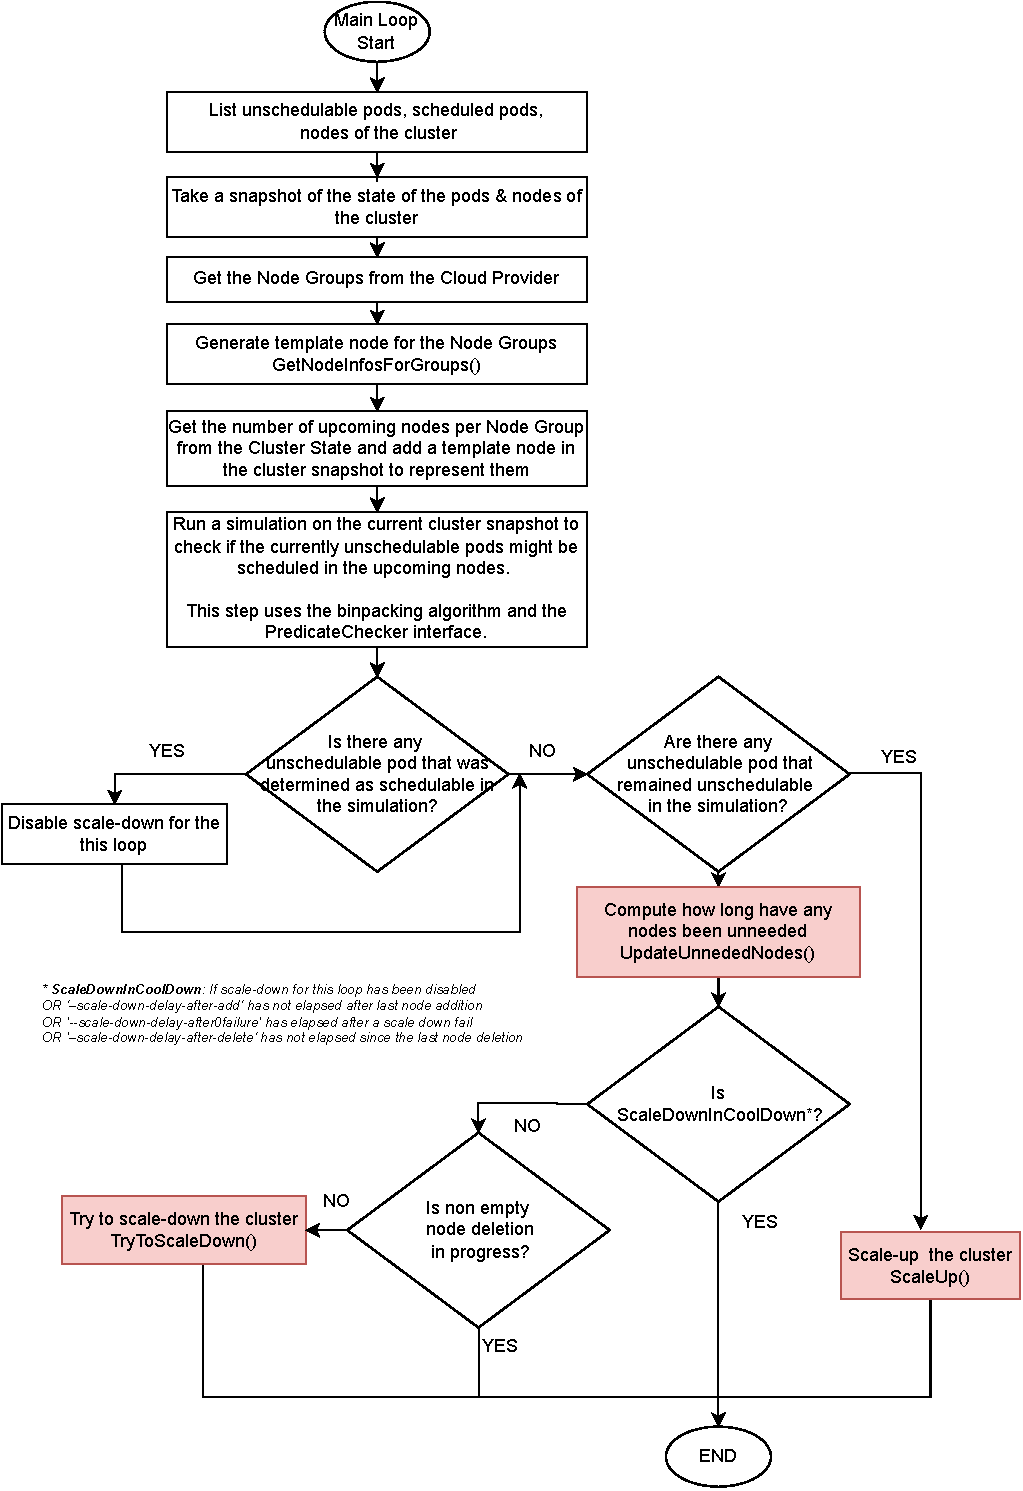
\includegraphics[width=\textwidth]{resources/autoscaler-main-loop.pdf}
      }
      \caption{Cluster Autoscaler:The main loop}
      \label{figure:autoscaler-main-loop}
\end{figure}


\subsection{Scale-Down}
\label{section:design-scale-down}
The Autoscaler tries to scale down the cluster if it did not attempt any
scale-up in the current run of the main loop. The scale-down procedure consists
of two distinct procedures:
\begin{enumerate}
      \tightlist
      \item \textit{Update unneeded nodes}: calculates which nodes have been
            unneeded and for how long.
      \item \textit{Try to scale down}: attempts to scale down the cluster by
            removing unneeded nodes.
\end{enumerate}

\begin{figure}[H]
      \centering
      \makebox[\textwidth][c]{
            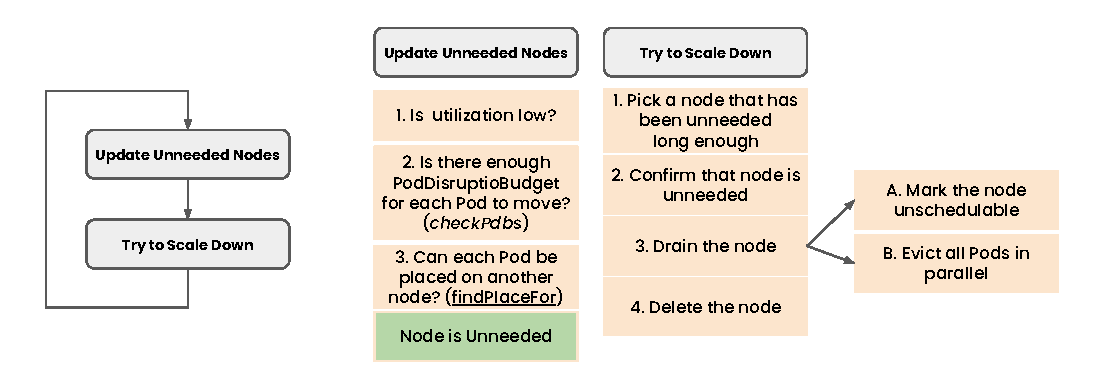
\includegraphics[width=1.1\textwidth]{resources/autoscaler-scale-down-process.pdf}
      }
      \caption{Cluster Autoscaler: Scale-down procedure}
      \label{figure:autoscaler-scale-down}
\end{figure}

We will use symbolic names to refer to various parameters of the Autoscaler in
our analysis, presented in Table \ref{table:symbolic-names-autoscaler}.
\begin{table}
      \begin{tabularx}{\linewidth}{|L|L|}
            \hline
            \textbf{Symbolic Name}        & \textbf{Description}                 \\ \hline
            scanInterval                  & How often cluster is reevaluated for
            scale up or down.
            \\
            \hline
            scaleDownDelayAfterAdd        & How long after scale up that scale
            down evaluation resumes. Defaults to 10 minutes. Configurable via
            the \co{--scale-down-delay-after-add} flag.                          \\
            \hline

            scaleDownDelayAfterDelete     & How long after node deletion that
            scale down evaluation resumes. Defaults to scanInterval.
            Configureable via the \co{--scale-down-delay-after-delete} flag.      \\
            \hline

            scaleDownDelayAfterFailure    & How long after scale down failure
            that scale down evaluation resumes. Defaults to 10 minutes.
            Configurable via the \co{--scale-down-delay-after-failure} flag.     \\
            \hline

            scaleDownUtilizationThreshold & Utilization threshold below which a
            node can be considered for scale down. Defaults to 0.5. Configurable
            via the \co{--scale-down-utilization-threshold} flag.                \\
            \hline

            scaleDownUnneededTime         & How long a ready node should be
            unneeded before it is eligible for scale down.  Defaults to 10
            minutes. Configurable via the \co{--scale-down-unneeded-time} flag.
            \\
            \hline

            scaleDownUnreadyTime          & How long an unready node should be
            unneeded before it is eligible for scale down.  Defaults to 20
            minutes. Configurable via the \co{--scale-down-unready-time} flag.
            \\
            \hline
      \end{tabularx}
      \caption{Symbolic names for various parameters of the Autoscaler used in our analysis}
      \label{table:symbolic-names-autoscaler}
\end{table}


\subsubsection{Update Unneeded Nodes Procedure}
The \textit{update unneeded nodes} procedure calculates which nodes of the
cluster have been unneeded and updates the Autoscaler's internal state with the
duration they have been unneeded. The Autoscaler considers a node
\textit{unneeded} if it meets all the following criteria:
\begin{itemize}
      \tightlist
      \item It is \textit{underutilized}, i.e., it has resource utilization
            below a specific threshold.
      \item The Pods that run on the node can be evicted (see section
            \ref{section:background-eviction}), i.e., their eviction is not
            blocked by any PodDisruptionBudgets.
      \item The Pods that run on the node can be moved to a different cluster
            node.
\end{itemize}
If a node does not meet the criteria, it is considered \textit{unremovable}.

To determine if an underutilized node is unneeded, the Autoscaler runs these
steps:
\begin{enumerate}
      \tightlist
      \item Calculate the Pods that must be moved if it removes the node.
      \item Check if any PodDisruptionBudgets block the eviction of any Pod. If
            so, the node is unremovable.
      \item Call \co{FindPlaceFor()} to find place for the Pods on a different
            node. \co{FindPlaceFor()} uses the
            \co{SchedulerBasedPredicateChecker} interface to determine if the
            Pod can be placed on any other node. It checks if the Pod can fit a
            node due to other scheduling constraints (CPU, memory), as well as
            if the Pod's volumes can be accessed from the node.
\end{enumerate}


The steps for  calculating the unneeded nodes are shown in
Algorithm~\ref{algo:update-unneeded}.

\subsubsection{Try to Scale Sown Procedure}

If a \textit{Ready} node remains unneeded for longer than
\co{scaleDownUnneededTime}, or an \textit{Unready} node remains unneeded for
longer than \co{scaleDownUnreadyTime} (see Table
\ref{table:symbolic-names-autoscaler} for the symbolic names) the Autoscaler
will consider the node as a candidate for deletion.

The Autoscaler makes a distinction between non-empty and empty nodes:
\begin{itemize}
      \tightlist
      \item \textit{Empty nodes}: nodes that run \textit{only} DaemonSet Pods.
            The Autoscaler removes them in bulk
      \item \textit{Non-empty nodes}: nodes that do not run only DaemonSet Pods.
            The Autoscaler removed them one by one to ensure that no Pods would
            be made unschedulable.
\end{itemize}

The algorithm for \co{TryToScaleDown()} is shown in
Algorithm~\ref{algorithm:try-scale-down}.

\paragraph*{Node removal} The node removal is executed as follows:
\begin{enumerate}
      \tightlist
      \item Add the \co{ToBeDeletedByClusterAutoscaler:NoSchedule} taint on the
            Node, essentially marking the node as unschedulable.
      \item Start draining the node by evicting in parallel all the Pods of the
            node. If any Pod can not be evicted due to a configured PDB, retry
            until the \co{MaxPodEvictionTimeout} exceeds.
      \item When all Pods are successfully evicted, ask the cloud provider to
            delete the node instance.
\end{enumerate}

The algorithm for the node removal is shown in
Algorithm~\ref{algorithm:node-delete}.


\clearpage
\begin{algorithm}[H]
    \caption{Cluster Autoscaler: Scale-down evaluation procedure}\label{alg:scale-down-evaluation}
    \SetKwIF{If}{ElseIf}{Else}{if~\endgraf}{\endgraf then}{else if}{else}{end if}%
    %\begin{minipage}{\textwidth}
    \begin{enumerate}[leftmargin=0cm]
        \tightlist
        \item Take a snapshot of the cluster Nodes, Pods, and PodDisruptionBudgets.
        \item \texttt{allNodes} \(\leftarrow\) List all the \co{Node} objects from the API Server.
        \item \texttt{scaleDownCandidates} \(\leftarrow\) Select nodes from
              \texttt{AllNodes} that belong to node groups that have not reached their
              minimum size.
        \item \texttt{podDestinations} \(\leftarrow\) \texttt{AllNodes};
              \texttt{podDestinations} represents the nodes that that may accept Pods in case a node is removed.
        \item Call \texttt{UpdateUnneededNodes()} with \texttt{podDestinations},
              and \texttt{scaleDownCandidates} as input, to calculate which nodes are
              unneeded an which ones are unremovable.
        \item \uIf{\begin{tabular}{@{\hspace*{1.0em}}l@{}}
                      the scale-down has been disabled for this loop                                           \\
                      % TODO: times in table
                      \textbf{OR} \co{scaleDownDelayAfterDelete} interval has not elapsed  \\
                      \textbf{OR} \co{scaleDownDelayAfterAdd} interval has not elapsed  \\
                      \textbf{OR} \co{scaleDownDelayAfterFailure} interval has not elapsed 
                  \end{tabular}}{
                  Don't scale-down the cluster. Autoscaler Status: \texttt{ScaleDownInCooldown}
              }
              \uElseIf{there is non empty node deletion in progress} {
                  Don't scale-down the cluster. Autoscaler Status: \texttt{ScaleDownInProgress}}
              \lElse{Try to scale down the cluster.}
    \end{enumerate}
    %\end{minipage}
\end{algorithm}


\begin{algorithm}[ht]
    \caption{Cluster Autoscaler: UpdateUnneededNodes() method}\label{algo:update-unneeded}
    \KwIn{\texttt{scaleDownCandidates}: a list of nodes that belong to
        node groups that have not reached their minimum size }
    \KwResult{Update the
        state of the Autoscaler with information about which nodes are unneeded}
    \begin{enumerate}[leftmargin=0.5cm]
        \tightlist
        \item For each node in \texttt{scaleDownCandidates}, call \texttt{checkNodeUtilization()}:
              \begin{enumerate}[]
                  \tightlist
                  \item \lIf{node has the ``ToBeDeletedByClusterAutoscaler'' taint}{ it is currently deleted, continue to next node}
                  \item \lIf{node has ``cluster-autoscaler.kubernetes.io/scale-down-disabled: true'' annotation}{continue to next node}
                  \item Calculate the utilization of the node.
                  \item \lIf{utilization is above threshold}{continue to next node}
                  \item Add the node \texttt{currentlyUnneededNodes}.
              \end{enumerate}
        \item \texttt{currentlyUnneededNonEmptyNodes} \lar From \texttt{currentlyUnneededNodes} select nodes that are not empty, i.e., they do not run only DaemonSet Pods.
        \item Call \texttt{findNodesToRemove(currentlyUnneededNonEmptyNodes)} to determine nodes that can be removed. For each node:
              \begin{enumerate}[]
                  \tightlist%        
                  \item Get the Pods that are running on the node and for each Pod:
                        \begin{enumerate}[leftmargin=0.5cm]
                            \tightlist
                            \item \lIf{the Pod has a Pod disruption budget that prevents its eviction}{the node is unremovable}
                            \item Call \texttt{findPlaceFor(pod)} to determine if it can be moved elsewhere.
                            \item \leIf{the Pod can not be moved elsewhere}{the
                                      node is unremovable}{the node can be removed, add it to
                                      \texttt{nodesToRemove}}
                        \end{enumerate}
              \end{enumerate}
        \item For each node in \texttt{nodesToRemove} update the state of the Autoscaler with the duration the node has been unneeded.
    \end{enumerate}
\end{algorithm}

\begin{algorithm}[ht]
\caption{Cluster Autoscaler: TryToScaleDown() method}\label{algorithm:try-scale-down}
    \KwIn{A list of unneeded nodes, as computed by UpdateUnneded() method}
    \KwResult{Scales-down the cluster}
\begin{enumerate}[leftmargin=0.5cm]
\item
  For each node in the unneeded nodes:

  \begin{enumerate}[leftmargin=0.5cm]
  \tightlist
  \item \lIf{If the node has the \texttt{cluster-autoscaler.kubernetes.io/scale-down-disabled}}{mark the node unremovable, reason \co{ScaleDownDisabledAnnotation}, go to next node.}
    \item
    \lIf{the node is \texttt{Ready}, and it has been underutilized for
    less than \texttt{ScaleDownUnneededTime}}{mark the node unremovable,
    reason \texttt{NotUnneededLongEnough}, continue to next node}
  \item
    \lIf{the node is \texttt{Unready}, and it has been underutilized for
    less than \texttt{ScaleDownUnreadyTime}}{mark the node unremovable,
    reason \texttt{NotUnreadyLongEnough}, continue to next node}
  \item
    Get the NodeGroup the node belongs to, get its \co{minSize} and current
    \co{size}, the number of node deletions in progress for the node group
    (\texttt{deletionsInProgress}).
  \item \lIf{\co{size} - \co{deletionsInProgress} $\leq$ \co{minSize}}{
    mark the node unremovable, reason \texttt{NodeGroupMinSizeReached},
    continue to next node}
  \end{enumerate}
  \item
  \co{candidates} \lar All the unneeded node that were not marked unremovable
  \item
    From \co{candidates}, try to scale-down as many as possible empty nodes.
  \item
    \texttt{nodesToRemove} \lar From the remaining candidates find nodes to
    remove (call \texttt{FindNodesToRemove()}).
  \item
    Pick a node from \texttt{nodesToRemove} and delete it
    (call \texttt{deleteNode()}) .
\end{enumerate}
\end{algorithm}
\begin{algorithm}[ht]
\caption{Cluster Autoscaler: deleteNode() method}\label{algorithm:node-delete}
    \KwIn{An unneeded Node of the Cluster to be deleted}
     \KwResult{Deletes the Node from the cluster and the Cloud Provider}
        \begin{enumerate}[leftmargin=0.5cm]
        \tightlist
        \item Add \co{ToBeDeletedByClusterAutoscaler:NoSchedule} taint on the
        Node to make the Node unschedulable.
        \item Drain the node; For each Pod (except for the DaemonSet Pods), in parallel:
            \begin{enumerate}
                \tightlist
                \item Send Eviction request
                \item \lWhile{the Eviction fails and for duration up to \co{MaxPodEvictionTimeout}}{retry the Eviction}

                Note: \co{MaxPodEvictionTimeout} is a hard-coded value equal to 2 minutes.
            \end{enumerate}
        \item \lIf{any of the Pods was not evicted successfully}{return error}
        \item \lIf{the node has any annotation with prefix
        \co{delay-deletion.cluster-autoscaler.kubernetes.io/}}{wait for up to
        \co{nodeDeletionDelayTimeout} for the annotation to be removed}
        \item Request from the Cloud Provider to delete the Node.
        \item \lIf{the Cloud Provider deletion fails}{return error}
        \end{enumerate}
\end{algorithm}


\clearpage
\subsection{Scale-Up}
\label{section:design-scale-up}
If the cluster has unschedulable Pods, the Autoscaler will try to help them by
adding new nodes to the cluster (\textit{scale-up}). A scale-up, essentially, is
the increase of the target size of one or more node groups. If multiple node
groups exist in the cluster, the cluster has to decide the following:
\begin{itemize}
      \tightlist
      \item Which node groups can help the unschedulable Pod run.
      \item How many nodes of the node group do the Pods need.
      \item If different node group scale-ups are feasible, which node group
            shall scale up.
\end{itemize}

As soon as the Autoscaler increases the target size of a node group, the cloud
provider will spin up new node instances, the new nodes will join the Kubernetes
cluster, and the scheduler will gradually scheduler the so far unschedulable
Pods to the new nodes.

The full algorithm for the \texttt{ScaleUp()} method is shown in
Algorithm~\ref{algorithm:scale-up}.

% TODO We show or is shown 
\paragraph*{Scale-up options}
To decide whether the scale-up of a node group would help the unschedulable Pod,
the Autoscaler runs the (roughly) following steps:
\begin{enumerate}
      \tightlist
      \item Take a snapshot of the cluster.
      \item Add a template node of the node group to the snapshot.
      \item Run a simulation, using the \co{SchedulerBasedPredicateChecker},
            whether the unschedulable Pod can be scheduled on the modified
            snapshot of the cluster.
      \item If the simulation determines that the Pod can be scheduled on the
            modified snapshot, use the \co{BinPackingNodeEstimator} to calculate
            how many nodes of that node group are needed.
\end{enumerate}

The option to scale up a specific node group with the number of needed nodes is
referred to as a ``\textit{scale-up option}''.

The complete algorithm to calculate a scale-up option is shown in Listing
\ref{algorithm:scaleup-options}.

\paragraph*{Scale-up strategy}

If multiple scale-up options, i.e., different node group scale-ups, can help the
unschedulable Pods, the Autoscaler decides which one is best using the
\co{Strategy} interface. There are various strategies, and the administrator can
configure the Autoscaler to use a desired one, e.g., the least cost option,
random strategy, etc.


\begin{algorithm}[ht]
    \caption{Cluster Autoscaler: ScaleUp() method}\label{alg:cap}
    \label{algorithm:scale-up} \KwIn{\co{pods}: the unschedulable Pods
        \\\co{snapshot}: the cluster snapshot } \KwResult{Adds extra nodes to
        accommodate the unschedulable Pods}
    \begin{enumerate}[leftmargin=0.5cm]
        \tightlist
        \item Build Pod equivalence groups - each Pod equivalence group consists
              of Pods that are managed by the same controller (same UUID) and have
              the same spec and labels.
        \item For each node group registered:
              \begin{enumerate}
                  \tightlist
                  \item Get its target size.
                  \item If the target size $\geq$ max size, go to the next node
                        group.
                  \item Create a template node for the node group.
                  \item Compute the expansion option for the node group, see
                        \co{ComputeExpansionsOption()}.
                  \item If any unschedulable Pod can be helped by adding a new
                        node of the node group, add the node group in the expansion
                        options list.
              \end{enumerate}
        \item If there are not any expansion options list, then do not trigger
              any scale-ups.
        \item Else, from the expansions options select one, according to the
              configured expansion strategy.
        \item Execute the selected scale up option: increase the target sizes of
              the corresponding node groups.
    \end{enumerate}
\end{algorithm}

\begin{algorithm}[ht]
    \caption{Cluster Autoscaler: ComputeExpansionsOption()
        algorithm}\label{algorithm:scaleup-options} \KwIn{\co{pods}: the unschedulable
        Pods \\\co{snapshot}: the cluster snapshot \\\co{template}: the template
        node of the node group} \KwResult{Computes if the scale-up of the node group
        would help any of the unschedulable Pods.}
    \begin{enumerate}[leftmargin=0.5cm]
        \tightlist
        \item
              For each Pod equivalence group:
              \begin{enumerate}
                  \tightlist
                  \item Get the sample Pod of the Pod equivalence group.
                  \item Add the template node in the cluster snapshot.
                  \item Call the Predicate Checker to check if any of the
                        unschedulable Pods can be scheduled in the new cluster snapshot.
                  \item If the sample Pod fits the new node in the cluster
                        simulation, append all the equivalent Pods in the list of Pods
                        that got helped (\co{options.Pods}).
              \end{enumerate}
        \item Call the bin-packing estimator to estimate how many nodes of
              the node group would be needed to help all the equivalent Pods.
        \item Return the \co{option}: a struct that indicates how many nodes of
              the node group are needed and which Pods would be helped.
    \end{enumerate}
\end{algorithm}



\clearpage
\subsection{Shortcomings \& Proposed Extensions}

In previous sections, we described the algorithms that govern the operations of
the Autoscaler; we will now identify their shortcomings.

\subsubsection{Scale-Down: Rok Volumes Can Be Migrated}
\label{section:design-autoscaler-unpinned}

When evaluating the scale-down of a node, the Autoscaler tries to find a place
for the Pods that run on the node in other cluster nodes. To do so, it calls the
\co{FindPlaceFor()} method, which in turn leverages the \co{PredicateChecker}
interface methods to determine if a Pod fits a node. The
\co{SchedulerBasedPredicateChecker} implementation of the interface runs the
VolumeBinding plugin's \co{Filter()} method to check if the volumes of the Pod
can be accessed from another node.


The PVs of the Rok storage class have node affinity that matches only with the
node where the volume was provisioned. Since the node affinity of the volumes
does not match any other in the cluster, the Autoscaler considers that the Pod
and its volume can not be moved on a different node, thus, marking the current
node as unremovable. The \co{SchedulerBasedPredicateChecker} does not know that
the Rok volumes have a mechanism to snapshot and recover them on a different
node [by unpinning them (snapshot + remove volume's node affinity, see section
            \ref{section:design-unpin}) and then pinning them (restoring the data) on
            another node ].

We propose the extension of the Autoscaler to simulate the Rok volumes as
unpinned (as if they do not have node affinity) when evaluating a scale-down
(and only then; in other cases, the volumes are retaining their node affinity).
With this extension, the Autoscaler will comprehend that the Rok volumes can
move anywhere in the cluster, and it can remove the node safely.

\subsubsection{Scale-Down: Coordinate With the Rok CSI Guard Mechanism}

As part of the Rok volume protection mechanism (see section
\ref{section:background-rok-csi-guard}), we deploy a \texttt{Deployment} object
for each node of the cluster, which creates a Pod per node (Rok CSI Guard)  with
strict node affinity that matches only the node it protects. The Autoscaler
tries \textit{to find place} to move this Pod. Since the Pod has strict node
affinity that matches only the current node, SchedulerBasedPredicateChecker
assumes that the Pod cannot be moved to a different node. Because of that, the
Autoscaler marks the node as unremovable. Of course, the Rok Operator will
remove the Pod after the Autoscaler removes the node, but the Autoscaler is
unaware of this fact.

Moreover,  the Autoscaler checks the PDB of the Guard Pod. The PDB of the Guard
Pod is configured to cause any evictions to fail. The Autoscaler notices that
and assumes that the Guard Pod will not be able to get safely evicted, thus,
marking the node unremovable. It is unaware that the Rok Operator will remove
them as soon as the scale-down starts and the Rok CSI  unpins all the local
volumes of the node.

We propose the extension of the Autoscaler so that it does not try to find a
place for the operator-managed ephemeral Guard Pods. Moreover, we extend the
Autoscaler to ignore the PDB of the Guard Pod. Still, the Autoscaler will be
aware that the Guard Pod exists, evicting it when it drains the node. This
eviction will fail as long as the PDB exists and the Autoscaler will retry,
delaying the deletion of the node.

To make things more obvious, here is the procedure that will take place with the
new design:


\begin{enumerate}
      \tightlist
      \item The Autoscaler evaluates a node for removal:
            \begin{enumerate}
                  \item It checks if the PDB allows the eviction of the Pods
                        running on the node, but it ignores the PDB of the Guard
                        Pod.
                  \item It tries to find a place for each Pod on a different
                        node, but it ignores the Guard Pod.
            \end{enumerate}
      \item The Autoscaler decides to remove the node.
      \item The Autoscaler adds the deletion taint on the node, effectively
            marking it as unschedulable for Pods.
      \item The Autoscaler sends eviction requests for each Pod to the API
            Server.
      \item The eviction of all the Pods --except for the Guard Pod-- succeeds.
      \item The Autoscaler keeps retrying to evict the Guard Pod, but the API
            Server responds that the eviction is not allowed due to the
            configured PDB.
      \item The Rok CSI Controller notices that the node is unschedulable and
            that no workload mounts the volumes, so it starts unpinning them.
      \item The Rok CSI Controller finishes the unpinning of the PVs.
      \item The Rok Operator removes the PodDisruptionBudget of the Guard Pod.
      \item The Autoscaler's request to evict the Guard Pod succeeds since the
            PDB was removed.
      \item The Autoscaler asks the cloud provider to delete the node.
      \item The Rok Operator removes the Rok CSI Guard \texttt{Deployment}
            object that corresponds to the removed node.
\end{enumerate}

Let us notice that the Autoscaler keeps retrying the eviction of the Guard Pod
for up to 2 minutes. That duration is a hard-coded timeout that might not be
enough in most cases. Taking a snapshot of the volume may last more than 2
minutes, depending on the size of the volume. It would be wise to use more sane
values and allow the user to cluster's admin to configure the value when
deploying the Autoscaler. To do so, we propose the extension of the Autoscaler
with a flag to configure the max pod eviction timeout.

\label{section:design-autoscaler-guards}


\subsubsection{Scale-Down: Consider Storage Capacity}

The Autoscaler shall check if the Rok volumes of a Pod can fit a node concerning
their requested storage capacity when evaluating a scale-down. As we have
explained, the Autoscaler used the \texttt{SchedulerBasedPredicateChecker}
interface in order to check if a Pod fits a node, which --among others-- calls
the VolumeBinding plugin's \co{Filter()} method.

We propose the extension of the SchedulerBasedPredicateChecker's VolumeBinding
plugin's \co{Filter} method: When evaluating if a Pod can be moved to a
different node, check if there is enough available storage on the node to move
the volumes.

Moreover, since the snapshotting and migration of a volume is a procedure that
costs in terms of time, the  Autoscaler shall not remove nodes with high storage
utilization, similarly to how it handles the CPU and memory resources. To
achieve this, we propose the extension of the Autoscaler with a new metric,
called the (Rok) ``\textit{storage utilization}'', defined as the ratio of the
used storage over the max storage capacity of the node. The Autoscaler will
compare this metric against a threshold configurable by the admin via a
corresponding flag; if the storage utilization exceeds the threshold, the node
will be considered unremovable.

\subsubsection{Scale-Down: Do Not Remove Unready Nodes}

A node that with status \co{Ready} can become \co{Unready} (or \co{NotReady}) if
a system problem on the node arises. Common reasons include lack of resources on
the node, a problem with the kubelet, an error related to kube-proxy, or a
networking problem in general.

The Autoscaler removes any unneeded Unready node after the
\texttt{scaleDownUnreadyTime} elapses. In the case of local volumes, we assume
that the node will always be in good condition, with all the systems up and
running and having network access, so Rok snapshots the local volumes to
Amazon's S3 remote storage. If that does not hold, removing a node will probably
cause any local data to be permanently lost.

The Autoscaler must not remove Unready nodes. The Unready nodes shall remain in
the cluster so that an administrator takes action to recover them from the
Unready state. We propose the extension of the Autoscaler with a flag to
explicitly disable the scale-down for nodes in \co{Unready} state and consider
them unremovable.

\subsubsection{Scale-Up: Consider Storage Capacity}
The Autoscaler does not know how much local storage is available when a new node
is spanned up and added to the cluster. The template node it creates from a live
node contains information only for the \textit{currently} free storage (of the
live node), reported on the capacity annotation by the storage driver (see the
proposed scheduler design, section \ref{section:capacity-annotation}). We need a
mechanism to know how much free storage a new node of a node group will have,
and the Autoscaler shall consider it in its simulations.

\paragraph*{Report max capacity}
Assuming that all the nodes in a node group have the same disk configuration and
max storage capacity, we can use the storage driver to report what the new
node's storage capacity would be on the \co{Node} objects. We propose the
extension of the Rok CSI Node component to report the max capacity of a node as
a label on the \co{Node} object. This label will be referred to as the
``\textit{max capacity label}'' \footnote{The \textit{Rok max capacity label}:
      rok.arrikto.com/max-instance-capacity}.

We use a label instead of an annotation because various cloud providers give the
cluster admins the option to pass labels to the node group node templates the
cloud provider plugin constructs. In case no live node for the node group
exists, the Autoscaler will construct the template from the cloud provider
plugin and have the configured admin labels on it.

At this point, let us distinguish the two reported quantities:
\begin{itemize}
      \tightlist
      \item \textit{capacity annotation}: the remaining free storage of a live
            node. The storage driver reports it, and the scheduler considers it
            when scheduling Pods.
      \item \textit{max capacity label}: the max storage capacity of the live
            node. i.e., the total storage capacity. That is a time constant
            value that depends on the node's disks.
\end{itemize}

For example, a node might have 200 Gi total storage (reported on the max
capacity label), and only 100 Gi out of them are free (reported on the capacity
annotation).

\paragraph*{Pass the max capacity information to the template}

For the Autoscaler to simulate the scheduling with capacity considerations, we
will import in the SchedulerBasedPredicateChecker the extended VolumeBinding
(see section \ref*{section:volume-plugin-extensions}).

The extended VolumeBinding plugin will look for the capacity of a template node
on the capacity annotation and not on the label. Since the template will get the
annotation from a live node, it will represent the currently free storage on the
live node instead of the max storage capacity. We need to sanitize the value and
set it to the actual max capacity. To do so, we propose the extension of the
sanitization mechanism of the Autoscaler to copy the max capacity label's value
to the capacity annotation. In this way, the template node's capacity annotation
will indicate the max capacity (total) storage of the new node of the node
group.

The sanitization mechanism shall set the capacity annotation to an infinitely
large value if the max capacity label does not exist. This design choice offers
the following advantages:
\begin{enumerate}
      \item The Autoscaler treats the node as if it had infinite storage
            capacity and will add a live node of the node group (scale-up). If
            the decision was wrong (\textit{false scale-up}), i.e., the added
            node does not have enough storage capacity for the Pod that
            triggered the scale-up, the scheduler of the cluster will not assign
            the Pod to the newly added node. As a result, the node will remain
            unneeded, and the Autoscaler will remove it after some time. The
            system will gradually fix the wrong decision.
      \item The wrong node addition allows the Autoscaler to learn the actual
            max capacity of the node. The Rok CSI driver gets the chance to run
            on the node, and the Autoscaler generates a template node from the
            live node, which contains accurate information for the max available
            capacity reported by the Rok CSI driver.
\end{enumerate}


\paragraph*{Wait for Rok CSI to run}

If a Pod triggers a scale-up because of the storage it requests, it may take a
reasonable time from the node addition till the Rok CSI driver starts running on
the node. As long as the Rok CSI is not running on the node, the corresponding
capacity annotation is not set on the \co{Node} object. The scheduler does not
schedule the Pod on the node since the absence of the annotation indicates the
storage is unavailable (see Section ~\ref{section:design-volume-binding}). The
Autoscaler runsthe scheduling simulation and decides that the Pod does not fit
the newly added node (since the live node has no capacity annotation), so it
triggers a new scale-up.

To resolve this issue, the Autoscaler must wait for the Rok CSI driver to run on
the newly added node. As long as the driver does not run on a new node (i.e.,
the node does not have the capacity label set), the Autoscaler shall replace the
node with an \textit{Unready} copy.

The Autoscaler treats Unready nodes as upcoming nodes (for a duration of up to
15 minutes): it replaces them with template nodes of the node group they belong
to in its simulations. The template node will have the capacity annotation set
as if the Rok CSI was running. The Autoscaler's simulation will assume that Pod
will be scheduled on the node when the Rok CSI is ready and running and will not
trigger any further scale-up.

We mentioned that the Autoscaler treats Unready node as upcoming for up to 15
minutes. That needs a bit of explanation. The Autoscaler gives the nodes a
reasonable amount to become fully Ready; after this duration, it will stop
replacing the Unready nodes with their template and will consider them
unschedulable in the simulation. If any Pods that relied on the node becoming
ready (in order to run there) still exist, they will now trigger another
scale-up. Of course, in the case of Rok, 15 minutes are more than enough for the
Rok CSI driver to become ready and start running.


\chapter{Implementation} \label{chapter:implementation}
In this chapter, we describe the implementation of the proposed design changes and the technologies used.

\section{Software Stack}

The proposed design involves many parts that we had to extend:
\begin{itemize}
      \tightlist
      \item Kubernetes Scheduler, written in Go.
      \item Kubernetes Cluster Autoscaler, written in Go.
      \item Rok CSI driver, written in Python.
\end{itemize}

It also introduces a new component, the Rok Scheduler webhook, which we wrote in
Go.

We build the components in a reproducible manner, using Docker containers for
the target language of each component. To describe and automate the build
process, we used Dockerfiles and Makefiles.

In order to deploy the components (Cluster Autoscaler, Rok Scheduler, Rok
Scheduler webhook) on the cluster, we write YAML manifests that use the
declarative API of Kubernetes to describe the necessary resources. To ease out
the manifests management, we use the \textit{Kustomize} tool. Kustomize is a
configuration management solution that leverages layering to preserve the base
settings of the applications and components by overlaying declarative YAML
artifacts (called patches) that selectively override default settings without
changing the original files.


\section{Extending the Rok CSI driver}

In order to extend the Rok CSI driver's node component with the capacity
reporting functionality, we introduce a new thread that periodically calculates
the capacity and updates the capacity on the \co{Node} object on the API Server. The
Python thread issues commands to the underlying Logical Volume Manager to fetch
the Rok VG size. We introduce an argument {\co{--capacity-poll-interval}} to
configure how long the thread waits before updating the storage capacity.


\lstinputlisting[label={listing:rok-capacity},language=Python,caption={The thread of Rok CSI driver that updates the available capacity}]{code/rok-capacity.python}

\section{Extending the Kubernetes Scheduler}

The VolumeBinding plugin of the Kubernetes Scheduler imports and uses the
\texttt{scheduling} package located at
\texttt{pkg/controller/volume/scheduling/scheduler\_binder.go}, in the
Kubernetes repo \footnote{\url{https://github.com/kubernetes/kubernetes}}. We
extend the package as follows:

\begin{itemize}
      \tightlist
      \item Introduce a \texttt{hasRokEnoughCapacity(claims\
            {[}{]}*v1.PersistentVolumeClaim,\ node\ *v1.Node)} method, which
            checks if there is enough capacity on the given \texttt{node} to
            provision all the specified Rok PVCs (\texttt{claims}). This method
            executes the following steps:
            \begin{enumerate}
                  \tightlist
                  \item Iterate through the given \co{claims}, and sum their
                        storage requests in
                        \texttt{totalRequestedCapacity}
                  \item Check if the given node has
                        \texttt{rok.arrikto.com/capacity} annotation.
                  \item If the annotation does not exist, or if it exists but is
                        not a valid int, returns \co{false}, which indicates the
                        PVCs can not be provisioned on the examined node.
                  \item If the annotation exists, fetch its value as
                        \texttt{nodeCapacityInBytes}.
                  \item If \texttt{totalRequestedCapacity} $\leq$
                        \texttt{nodeCapacityInBytes} return true, otherwise
                        false.
            \end{enumerate}
            The implementation of the method is exposed in listing
            \ref{listing:hasrokenough}.
      \item Extend the \texttt{checkVolumeProvisions()} method of the
            \co{VolumeBinding} plugin to gather all the Rok PVCs, (PVCs
            provisioned by \texttt{rok.arrikto.com}), and pass them to
            \texttt{hasRokEnoughCapacity()}, in order to check if there is
            enough capacity for all of them to be provisioned on a selected
            node. The implementation is show at Listing
            \ref{listing:checkvolumeprovisions}.
      \item Treat the case that the \texttt{rok.arrikto.com/capacity} does not
            exist as \texttt{zero} capacity, i.e., the volumes can not be
            provisioned.
\end{itemize}

\lstinputlisting[label={listing:hasrokenough},language=Golang,caption={Implementation of the hasRokEnoughCapacity() method}]{code/scheduler-rok-has-enough.go}
\lstinputlisting[label={listing:checkvolumeprovisions},language=Golang,caption={Extension of the checkVolumeProvisions() method}]{code/scheduler-volume-binding.go}

We compile the Rok Scheduler and build its Docker image using the Makefile the
upstream project provides. We use YAML manifests and the Kustomize tool to
deploy the Rok Scheduler as a \co{Deployment} along with any other RBAC
resources it needs for its operation.

\section{Implementing the Rok Scheduler Webhook}

We implement the Rok Scheduler webhook that will mutate the Pods to use the Rok
Scheduler, in a manner it can be reused and easily configured. 

We expose the following configuration options:
\begin{itemize}
      \item {\co{--annotation-optout}}:  Annotation key that if present
            on the Pod, the Pod will not be mutated. The default value is
            \co{arrikto.com/skip-rok-scheduler-webhook}. This parameters allows
            the user to skip the mutation of a Pod in the webhook server, even
            though the API server admitted that Pod for mutation. We will refer
            to it as the ``\textit{opt-out annotation}''.
      \item {\co{--namespaces-optin}}: A comma-separated list of
            namespaces or namespaces globs. If a Pod matches against one of
            these namespaces it will get mutated. The default value is
            \co{``*''}, which matches against all namespaces. We will refer to
            it as the ``\textit{opt-in namespaces}''.
      \item {\co{--scheduler-name}}: The name of the scheduler that will
            be set on the Pod. The default  value is \co{rok-scheduler}.
\end{itemize}
For a complete list of arguments, see the \co{main()} method of the webhook in
Listing \ref{listing:webhook-main}.

The \co{Handle()} method of the webhook handles a single admission request as
follows:
\begin{enumerate}
      \tightlist
      \item If the Pod it has the opt-out annotation, do not mutate it.
      \item Check the namespace of the Pod against each namespace glob. If
            the namespace does not match any glob, do not mutate it.
      \item In all other cases, mutate the Pod by adding the scheduler name on
            its \\ \co{spec.SchedulerName} field.
\end{enumerate}

For the full implementation of the method, see Listing
\ref{listing:webhook-handle}.

We implement the Rok Scheduler Webhook using the \co{webhook} package of the
controller-runtime library of Go. The Kubernetes controller-runtime is a set of
go libraries for building controllers. For implementing the glob functionality
of the \co{--namespaces-optin} flag, we used the \co{glob} module of Go. 

Finally, in order for the Pods to be admitted and sent to the webhook, we
instruct the API Server to do so by creating a \co{MutatingWebhookConfiguration}
object (see Listing \ref{listing:webhook-object}). The
MutatingWebhookConfiguration we specify admits any newly created Pods in
namespaces that match the specific namespace selector. The namespace selector
matches against any namespaces that have the label \co{control‐plane: kubeflow}.
We chose to admit Pods only in this namespace since the workload we want to
admit is created in that namespace, but of course, the Pods in any other
namespace can be admitted. The MutatingWebhookConfiguration specifies that the
API server contacts the webhook server at the \co{/mutate} endpoint. It also
specifies a \co{Fail} failure policy so that if the webhook crashes or stops
responding, the creation of new Pods will fail. That is important to ensure
every single Pod is admitted and mutated with the scheduler name.

\lstinputlisting[label={listing:webhook-main},language=Golang,caption={The main() method of the Rok Scheduler Webhook}]{code/mutating-webhook-main.go}
\lstinputlisting[label={listing:webhook-handle},language=Golang,caption={The Handle() method the Rok Scheduler Webhook}]{code/webhook.go}
\lstinputlisting[label={listing:webhook-object},language=yaml,caption={The Rok Scheduler's MutatingWebhookConfiguration}]{code/mutating-webhook.yaml}

To build the Rok Scheduler Webhook and its Docker image, we create a Dockerfile
that instructs the docker to build the binary inside a container that has the
required \texttt{Golang} dependencies. 

We deploy the Rok Scheduler and the Rok Scheduler as \co{Deployment} resources
(see \ref{section:deployment}). The manifests also specify other necessary
resources, such as Roles, RoleBindings, ServiceAccounts, ConfigMaps.

\section{Extending the Cluster Autoscaler}

\subsection{Scale-Down: Rok Volumes Can Be Migrated}
\label{section:implementation-migration}
As explained in the design proposal (see
\ref{section:design-autoscaler-unpinned}), we extend the Cluster Autoscaler to
treat the local volumes of the Rok Storage class as unpinned, i.e., as if they
have no affinities, when evaluating a possible scale-down. In all other cases,
the local volumes shall be evaluated as is, pinned, i.e., having their existing
node affinities. 

To implement the design, we extend the CheckPredicates interface's method with
an extra boolean argument, called \co{simulateUnpinnedVolumes}. We pass down
information from the PredicateChecker methods to the VolumeBinding plugin's
\co{checkBoundClaims()} method. The SchedulerBasedPredicateChecker creates a
\co{cycleState} (see section \ref{section:cycle-state} struct that the plugins
it runs can use for storing data. We extend the \co{cycleState}  with the same
boolean \co{simulateUnpinnedVolumes} field to pass down to the VolumeBinding
plugin information. The full flow of the information whether to simulate
unpinned volumes or not is illustrated in Figure ~\ref{fig:flow-simulate}.

\begin{figure}[ht]
      \centering
      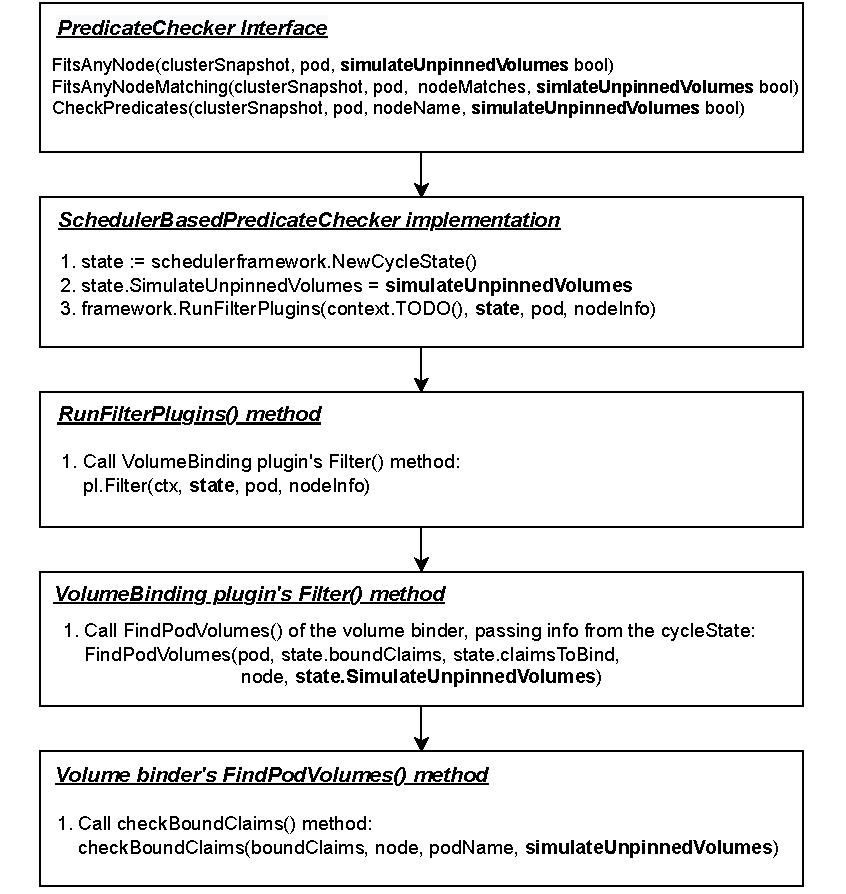
\includegraphics[width=0.8\textwidth]{resources/simulate-unpinned-flow.pdf}
      \caption{The flow of simulateUnpinnedVolumes information}
      \label{fig:flow-simulate}
\end{figure}


We extend the \co{checkBoundClaims()} method, so that if the Rok volumes are
simulated as unpinned (\co{simulateUnpinnedVolumes} is set to \co{true}), it
gathers all the Rok local volumes, and appends them to \co{claimsToProvision},
i.e, it treats them as if they were unbound volumes, in order to check if there
is enough capacity (see (\co{checkVolumeProvision()}) for the volumes to be
provisioned on the examined node. Of course, this approach only checks if the
Rok volumes of a Pod alone can be moved to a different node; it does not ensure
that all the Pods of the node can fit on a different node with regards to their
local storage requests. Listing \ref{listing:check-bound-claims} presents the
code lines that extend the functionality of \co{checkBoundClaims}.

\lstinputlisting[language=Golang,label={listing:check-bound-claims},caption={Extending the logic of checkBoundClaims() when volumes are simulated as unpinned}]{code/find-pod-volumes.go}


\subsection{Scale-Down: Coordinate With the Rok CSI Guard Mechanism}


To implement the design proposal (see section
\ref{section:design-autoscaler-guards}) we implement the following changes,
according to the proposed design:
\begin{itemize}
      \tightlist
      \item Extend the \co{findPlaceFor()} method to ignore the Rok CSI
            Guard Pods and not try to find a place for them on a different node.
      \item Extend the \co{checkPdbs()} method to not check the PodDisruptionBudgets
            of the Rok CSI Guard Pods.
      \item We introduce a flag \co{--max-pod-eviction-time}  so that the
      cluster admins can configure the maximum time Autoscaler tries to evict a Pod
      before giving up.
\end{itemize}

\lstinputlisting[language=Golang,label={listing:ignore-guard},caption={Ignore Rok CSI Guard Pods and their PDBs in scale-down evaluation}]{code/find-place-for.go}

%TODO: code snippet flag


\subsection{Scale-Down: Consider Storage Capacity}
We already covered in section \ref{section:implementation-migration} how we
extended the Autoscaler to simulate the Rok volumes as unpinned when scaling
down and also check if there is enough capacity for each Pod on a different
node.

We also extend the Autoscaler to calculate storage utilization and take it into
consideration when scaling down, by introducing a new flag
``--scale-down-rok-storage-utilization-threshold'' flag with default value
``0.5'' and a \co{CalculateUtilizationOfRokStorage()} method. This method
fetches the values from the capacity annotation and the max capacity label of
the \co{Node} object and calculates the storage utilization. Moreover, we extend
the \co{checkNodeUtilization()} method of the Autoscaler to mark any nodes that
have storage utilization over the storage threshold as unremovable. The
implementation can is shown in Listings \ref{listing:storage-util} and
\ref{listing:node-utilization}.

\lstinputlisting[label={listing:storage-util},language=Golang,caption={Calculate Rok storage utilization}]{code/rok-utilization.go}
\lstinputlisting[label={listing:node-utilization},language=Golang,caption={Mark nodes with high Rok storage utilization as unremovable}]{code/rok-utilization-threshold.go}


\subsection{Scale-Down: Do Not Remove Unready Nodes}

To implement the proposed design and configure the Autoscaler to not removed
unready nodes, we extend the \texttt{--scale-down-unready-time} of the
Autoscaler to accept negative values; if a negative value is provided, then the
scale-down of unready nodes will be disabled.

\subsection{Scale-Up: Consider Storage Capacity}

\paragraph*{Pass the max capacity information to the template}
To implement the scale-up design, we introduce a method
\co{sanitizeRokStorageAnnotations()} that copies the value of the max capacity
label of the \texttt{Node} object to its capacity annotation. If the label does
not exist, it set the capacity annotation to the max 64 bit number.We extend the
\co{sanitizeTemplateNode()} method to call \co{sanitizeRokStorageAnnotations} as
part of the sanitization process.

The implementation of this functionality is shown in Listings
\ref{listing:sanitize-rok} and \ref{listing:sanitize}.

\lstinputlisting[language=Golang,label={listing:sanitize-rok},caption={sanitizeRokStorageAnnotations() method}]{code/scale-up-capacity-label.go}
\lstinputlisting[language=Golang,label={listing:sanitize},caption={Extend sanitizeTemplateNode() to sanitize the Rok storage annotations}]{code/note-template-capacity.go}

\paragraph*{Wait for Rok CSI to run}

We implement this design change by introducing a
\co{FilterOutNodesWithUnreadyCSI()} method to check if a node has the capacity
annotation set. If not, it is implied that the Rok CSI driver is not running on
the node, and it replaces the node with an unready copy. We extend the
\co{obtainNodeLists()} method, to call the \co{FilterOutNodesWithUnreadyCSI}.

Listings \ref{listing:unready-csi} and \ref{listing:unready-csi-obtain} present
the code lines that implement this functionality.

\lstinputlisting[label={listing:unready-csi},language=Golang,caption={FilterOutNodesWithUnreadyCSI() method}]{code/unready-csi.go}
\lstinputlisting[label={listing:unready-csi-obtain},language=Golang,caption={Extend ObtainNodesLit() method to return nodes with unready Rok CSI}]{code/obtain-nodes-list.go}

\chapter{Conclusion} \label{chapter:conclusion}

Our journey has finally reached its end. In this chapter, we will restate our
contributions and summarize what our mechanism offers. Finally, we will close
this thesis by mentioning future work that can be done to enrich our mechanism
and bring it to its full potential.

\section{Concluding Remarks} \label{section:conclusion_concluding_remarks}

All in all, the primary goal of this thesis was to implement a design that would
enable seamless cluster autoscaling and scheduling with local persistent
storage. Not only did we achieve this goal, but our implementation was
successfully deployed to large production clusters of enterprises that requested
the feature.

Although the design we implemented is coupled with the Rok software --since it
provides an efficient mechanism for migrating local volumes around a cluster--,
the concepts and the design can be generalized to work with any other local
storage system. Our long-term goal, which extends beyond the context of this
thesis, is to generalize the design and push it upstream. That is a process that
we started to be involved in; we attend the meetings of the Kubernetes Storage
\footnote{https://github.com/kubernetes/community/blob/master/sig-storage/README.md}
and Autoscaling
\footnote{https://github.com/kubernetes/community/blob/master/sig-autoscaling/README.md}
Special Interest Groups, interacted with them on GitHub and plan to contribute
the whole design upstream actively. At the moment this text is written, we have
a few first Pull Requests merged
\footnote{https://github.com/kubernetes/autoscaler/pull/4877}
\footnote{https://github.com/kubernetes/autoscaler/pull/4842}.

\section{Future Work} \label{section:conclusion_future_work}

So far, we have implemented various enhancements for the Kubernetes Scheduler
and the Cluster Autoscaler, but there is always room for improvement. Since this
is an iterative process, in next iterations, we would like to offer these
enhancements:

\begin{itemize}
      \item Extend the Scheduler to reserve the storage (in the \co{Reserve}
            phase of the scheduling cycle) when scheduling a Pod to prevent race
            conditions.
      \item Extend the Cluster Autoscaler to consider the storage needed for the
            PVCs of multiple Pods when scaling down. The current design only
            checks if a single Pod's PVs can fit a node, but not if the PVs of
            multiple Pods fit a node. Although a wrong decision to scale down
            will be reverted by a subsequent scale-up, taking the decision would
            be much more effective.
      \item Extend the current implementation of the \co{Estimator} interface,
            i.e., the \co{BinPackingEstimator}, to consider the storage and
            calculate how many nodes are needed for the storage requests of
            multiple Pods of a StatefulSet. The current design adds nodes one by
            one till all the Pods get the requested storage. It would be much
            more efficient to know the number of nodes needed beforehand and add
            them to the cluster all at once.
\end{itemize}

Finally, as we already mentioned, our high-priority goal is to merge this work
upstream.

\backmatter

% https://tex.stackexchange.com/questions/17653/how-to-list-all-bibliography-entries-without-citing
\nocite{*}
\phantomsection
\addcontentsline{toc}{chapter}{\bibname}
% gregth: change biobliography style
% https://tex.stackexchange.com/questions/420588/numbered-citations-in-latex
%\bibliographystyle{./styles/amsalpha}
\bibliographystyle{plain}
\bibliography{thesis-biblio}

\appendix

%\chapter{Publications} \label{chapter:publications}

Αρνάκι άσπρο και παχύ, της μάνας του καμάρι.

\end{document}
